\documentclass[11pt,reqno]{amsart}
\usepackage[a4paper,margin=27mm]{geometry}
\usepackage{amsmath,amssymb}
\usepackage[utf8]{inputenc}
\usepackage[T1]{fontenc}
\usepackage{mathptmx}
\usepackage{amsthm}
\usepackage{mathrsfs}
\usepackage{graphicx}
\usepackage{booktabs}
\usepackage{multirow,longtable}
\usepackage{array}
\usepackage{tikz}
\usetikzlibrary{arrows.meta,positioning,calc,matrix,shapes.geometric,decorations.pathreplacing}
\usepackage{xcolor}
\usepackage{enumitem}
\usepackage[colorlinks=true,linkcolor=blue!50!black,citecolor=blue!50!black,urlcolor=blue!50!black]{hyperref}
\usepackage{orcidlink}
\usepackage[protrusion=true,expansion=false]{microtype}
\usepackage{xurl}
% shims for the two-column source: one-column journal build
\usepackage{changepage}
\newenvironment{widetext}{\begin{adjustwidth}{-16mm}{-16mm}}{\end{adjustwidth}}
\newenvironment{ruledtabular}{\begin{adjustwidth}{-16mm}{-16mm}\footnotesize\setlength{\tabcolsep}{3.5pt}\centering}{\end{adjustwidth}}
\newcommand{\colrule}{\midrule}
\raggedbottom
\makeatletter
\renewcommand\subsection{\@startsection{subsection}{2}\z@{.6\linespacing\@plus.7\linespacing}{.3\linespacing}{\normalfont\bfseries}}
\makeatother
\newcommand{\affiliation}[1]{}
\providecommand{\keywordsjournal}[1]{}
\numberwithin{equation}{section}
\allowdisplaybreaks

\theoremstyle{plain}
\newtheorem{theorem}{Theorem}[section]
\newtheorem{proposition}[theorem]{Proposition}
\newtheorem{lemma}[theorem]{Lemma}
\newtheorem{corollary}[theorem]{Corollary}
\theoremstyle{definition}
\newtheorem{definition}[theorem]{Definition}
\newtheorem{remark}[theorem]{Remark}
\newtheorem{setup}[theorem]{Setting}

\newcommand{\QQ}{\mathbb{Q}}
\newcommand{\ZZ}{\mathbb{Z}}
\newcommand{\RR}{\mathbb{R}}
\newcommand{\CC}{\mathbb{C}}
\newcommand{\PP}{\mathbb{P}}
\newcommand{\Hdg}{\mathrm{Hdg}}
\newcommand{\Hg}{\mathrm{Hg}}
\newcommand{\NS}{\mathrm{NS}}
\newcommand{\Ab}{\mathrm{Ab}}
\newcommand{\Ext}{\mathrm{Ext}}
\newcommand{\Hom}{\mathrm{Hom}}
\newcommand{\End}{\mathrm{End}}
\newcommand{\ch}{\mathrm{ch}}
\newcommand{\Tr}{\mathrm{Tr}}
\newcommand{\trd}{\mathrm{trd}}
\newcommand{\nrd}{\mathrm{nrd}}
\newcommand{\Gal}{\mathrm{Gal}}
\newcommand{\Pic}{\mathrm{Pic}}
\newcommand{\Sp}{\mathrm{Sp}}
\newcommand{\SO}{\mathrm{SO}}
\newcommand{\SU}{\mathrm{SU}}
\newcommand{\SL}{\mathrm{SL}}
\tolerance=2000
\emergencystretch=3em
\hbadness=2500
\hfuzz=1pt
\newcommand{\Alg}{\mathrm{Alg}}
\newcommand{\cD}{\mathcal{D}}
\newcommand{\cA}{\mathcal{A}}
\newcommand{\cS}{\mathcal{S}}
\newcommand{\cH}{\mathcal{H}}
\newcommand{\HC}{\mathbf{HC}}
\newcommand{\AB}{\mathbf{AB}}
\newcommand{\Fii}{\texorpdfstring{\textup{(F2)}}{(F2)}}
\newcommand{\Fiii}{\texorpdfstring{\textup{(F3$'$)}}{(F3')}}
\newcommand{\codeRelease}{https://github.com/creelie/fermat-hodge-/releases/tag/v3.1.0}
\newcommand{\leancount}{four hundred and nine}
\providecommand{\Q}{\QQ}
\providecommand{\C}{\CC}
\providecommand{\R}{\RR}
\providecommand{\CH}{\operatorname{CH}}
\providecommand{\Res}{\operatorname{Res}}
\providecommand{\Ftwo}{\Fii}
\providecommand{\Fthree}{\Fiii}

\newcommand{\archiveDOI}{10.5281/zenodo.23439577}
\newcommand{\archiveLabel}{Zenodo concept DOI}
\InputIfFileExists{archive-imprint.tex}{}{}
\begin{document}

\title[Algebraic Transfer of Hodge Classes]{Algebraic Transfer and Propagation of Hodge Classes}

\author{Deep Bhattacharjee\,\orcidlink{0000-0003-0466-750X}}
\address{Formerly, Electro-Gravitational Space Propulsion Laboratory (EGSPL), Bhubaneswar, Odisha 751030, India; Formerly, University of Calcutta (Heramba Chandra College), 23/49 Gariahat Road, Golpark, Kolkata 700029, West Bengal, India}
\email{d.bhattacharjee@erl-forschung.de}
\email{itsdeep@live.com}
\email{egspl@proton.me}
\thanks{Corresponding author: Deep Bhattacharjee (\nolinkurl{d.bhattacharjee@erl-forschung.de}).}
\thanks{An earlier version of this paper is the Hexagon preprint 2610.00315v2, \url{https://hexagonmath.org/2610.00315v2}. This version revises it substantially.}
\thanks{Repository: \url{https://github.com/creelie/fermat-hodge-}. Release v3.1.0: \url{\codeRelease}. \archiveLabel: \href{https://doi.org/\archiveDOI}{\archiveDOI}.}

\author{Ushashi Bhattacharya\,\orcidlink{0009-0002-2254-3914}}
\address{Formerly, National Taiwan University, Taipei 106319, Taiwan}
\email{rai.bhattacharya.in@gmail.com}

\date{Version 7, revised 7 November 2026. Research release 3.1.0.}

\subjclass[2020]{14C30, 14K20, 14J28, 11E12}
\keywords{Hodge conjecture; abelian varieties; Weil classes; K3 surfaces}

\begin{abstract}
We construct algebraic correspondences at matched complex-multiplication fibres and explicit projectors for primitive codimension-two Hodge classes. We derive exact transfer formulas under blow-ups and finite covers, and a bounded-degree criterion that promotes special-fibre cycles to a relative algebraic cycle. The real-multiplication and Weil-class constructions of earlier versions are retained. The universal statements F2 and F3\( {}'\), and hence the general rational Hodge conjecture, remain unproved.
\end{abstract}

\maketitle
\enlargethispage{8pt}
\setcounter{tocdepth}{1}
\tableofcontents

\section{Introduction}\label{sec:intro}

The Hodge conjecture asks that every rational cohomology class of type $(p,p)$ on a smooth complex projective variety be a rational combination of classes of algebraic subvarieties.\footnote{An earlier preprint of the authors, \emph{Relative secant cycles and Hodge classes}, Preprints.org (2026), \nolinkurl{doi:10.20944/preprints202602.0462.v5} \cite{BB26}, claimed a proof of the Hodge conjecture that does not hold, and the present paper replaces it. The secant variety $\mathrm{Sec}^{n}(A^{\vee})$ contains $A^{\vee}$, so the cycle $\Sigma\cap A^{\vee}$ of its Definition~3 is $A^{\vee}$ itself, whose Fourier--Mukai transform is a skyscraper sheaf with no component in degree $2n$, contrary to its Lemma~4. The Weil classes span a $2$-dimensional space on which $K^{\times}$ acts by $\tau\mapsto\tau^{2n}$, while $\eta^{n}$ has character $N(\tau)^{n}$, contrary to its Propositions~1 and~2. Its general case (Theorem~12) applies the Kuga--Satake construction outside Hodge structures of K3 type and assumes the Kuga--Satake correspondence algebraic, which is open. Section~\ref{sec:earlier} lists every point at which that preprint fails.} Hodge raised it in 1950 \cite{Hod50}; Lefschetz had proved it for divisors \cite{Lef24}. It is known in a scattered family of cases and open in general. This paper does three things. It proves that the conjecture is equivalent to two statements about abelian varieties. It proves a closed-stratum dichotomy for the algebraic locus of a flat Hodge class and density for the particular period families supplied with algebraic CM seeds. A density statement for arbitrary smooth projective families is not asserted. And it builds, at the first class each statement has to reach, an explicit object, proves what that object does, and names the step at which it stops. The conjecture does not close here. What the paper adds is a complete account of where the two remaining statements live, two new theorems on real multiplication, by $\QQ(\sqrt6)$ on K3 surfaces and by the cyclic cubic fields $\QQ(\zeta_{7})^{+}$ and $\QQ(\zeta_{9})^{+}$ on the surfaces of Mumford type, the second of which closes the first two cases of the frontier of \cite{BMB26}, and three constructions carried to the point where the next step is a single stated question. Figure~\ref{fig:roadmap} draws this plan.

\begin{figure*}[t]
\centering
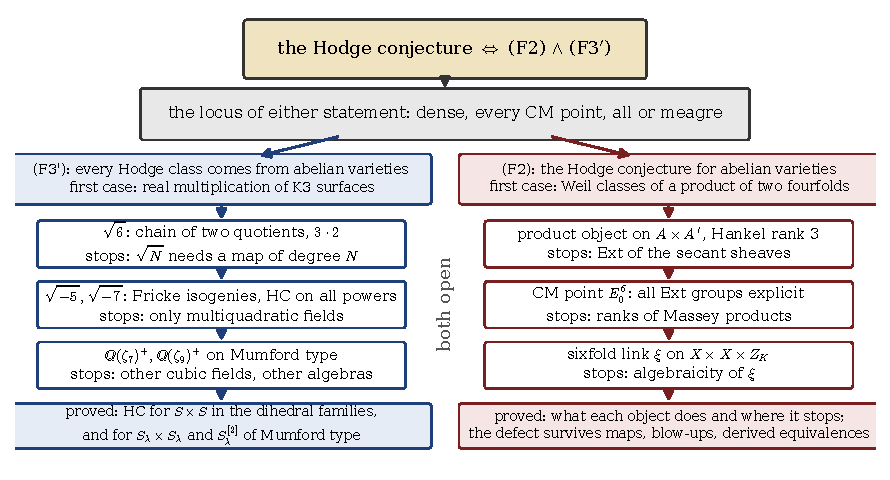
\includegraphics[width=0.96\textwidth]{figures/fig_roadmap}
\caption{The plan of the paper. The conjecture is equivalent to \Fii{} and \Fiii{} (Theorem~\ref{thm:intro-reduction}, Proposition~\ref{prop:minimal}); the algebraic locus is all or meagre, with density proved for the named period families (Section~\ref{sec:loci}). For \Fiii{} the first class is the real multiplication of K3 surfaces: the chain of quotients for $\sqrt6$ (Theorem~\ref{thm:sqrt6}), the Fricke isogenies, complex multiplications by $\QQ(\sqrt{-5})$ and $\QQ(\sqrt{-7})$ that settle every power (Theorem~\ref{thm:fricke}), the cyclic cubic fields on the surfaces of Mumford type (Theorem~\ref{thm:zeta9}), and the steps at which each stops (Propositions~\ref{prop:structure} and~\ref{prop:cubicstop}). For \Fii{} the first class is the Weil classes of a product of two fourfolds: the product object (Theorem~\ref{thm:product}, stopping at Proposition~\ref{prop:convolution}), the point of complex multiplication (Lemma~\ref{lem:cmext}, Proposition~\ref{prop:separated}, stopping at Section~\ref{ssec:f2stop1}) and the sixfold link (Theorem~\ref{thm:link}, stopping at Section~\ref{ssec:f2stop2}); the defect survives the operations of Proposition~\ref{prop:surgery}.}
\label{fig:roadmap}
\end{figure*}

\subsection{The two statements}

Write $\HC$ for the Hodge conjecture for all smooth complex projective varieties and $\AB$ for its restriction to abelian varieties. For a smooth projective variety $X$ and an integer $p$ let $\Hdg^{p}(X)$ be the Hodge classes of degree $2p$, and let $\Ab^{p}(X)\subseteq\Hdg^{p}(X)$ be the span of the classes $\Gamma_{*}\gamma$, where $B$ runs over the complex abelian varieties (the point included), $\gamma$ over the Hodge classes on $B$, and $\Gamma$ over the algebraic correspondences from $B$ to $X$. The two statements are
\begin{itemize}[leftmargin=2.4em,itemsep=2pt]
\item[\Fii] every Hodge class on every complex abelian variety is algebraic, in the form in which it first appears in the closure computation of \cite{BMB26}: the Hodge classes of the smallest known instance, the exceptional classes on the square of a Mumford fourfold, are algebraic together with everything that can be built from them;
\item[\Fiii] $\Hdg^{p}(X)=\Ab^{p}(X)$ for every $X$ and every $p$: every Hodge class is algebraic modulo the images, under algebraic correspondences, of Hodge classes of abelian varieties.
\end{itemize}

\begin{theorem}[Reduction]\label{thm:intro-reduction}
$\HC$ holds if and only if \Fii{} and \Fiii{} both hold; \Fii{} is equivalent to $\AB$, and \Fiii{} holds on every abelian variety, on every variety dominated by a product of curves or by an abelian variety, and on every variety in degrees $2p$ with $p\in\{0,1,\dim X-1,\dim X\}$.
\end{theorem}

The content of the theorem is in the second sentence: \Fii{} is not a special case of the conjecture for abelian varieties but the whole of it, carried by its hardest classes, and \Fiii{} is exactly what the conjecture asks of the part of the cohomology of $X$ that no abelian variety reaches. Section~\ref{sec:reduction} proves it and places the two statements in the closure graph of the known reductions, with the Lefschetz standard conjecture, Andr\'e's motivated classes and the variational Hodge conjecture as the other nodes (Fig.~\ref{fig:graph}).

\subsection{The shape of the known locus}

For a smooth projective family $\pi\colon\mathcal{X}\to S$ and a flat Hodge class $\xi$ let $\Sigma(\xi)\subseteq S$ be the set of points at which $\xi$ is algebraic.

\begin{theorem}[Dichotomy and propagation]\label{thm:intro-loci}
\leavevmode
\begin{enumerate}[label=\textup{(\roman*)},leftmargin=2.4em,itemsep=2pt]
\item $\Sigma(\xi)$ is a countable union of Zariski closed subsets of $S$, and either $\Sigma(\xi)=S$ or $\Sigma(\xi)$ is meagre.
\item \Fii{} holds if and only if, for every polarised abelian scheme and every flat Hodge class $\xi$, algebraicity of $\xi$ at one point of complex multiplication forces $\Sigma(\xi)=S$.
\item For the Weil classes of every CM field, every $n\ge2$ and every discriminant, $\Sigma(\xi)$ contains an explicit point of complex multiplication and is dense.
\item \Fiii{} holds for $X$ in degree $2p$ if and only if a Hodge complement of the abelian part of $H^{2p}(X,\QQ)$ carries no nonzero Hodge class.
\end{enumerate}
\end{theorem}

In the Weil families and in the matched sixfold-link family constructed below, explicit cycles give a dense algebraic locus. The countable closed-stratum description holds more generally, but does not by itself give density or propagation for an arbitrary class or family. Figure~\ref{fig:locus} draws it. Section~\ref{sec:loci} proves the theorem, after \cite{BMB26}, whose argument we rewrite in the generality needed here.

\subsection{Constructions at the first class}

The rest of the paper is constructive. At each statement we go to the first class that is not known and build the object that would make it algebraic.

At \Fiii{} the first class lives on powers of a K3 surface $S$ with real multiplication: the transcendental lattice $T(S)_{\QQ}$ is a vector space over a totally real field $E=\End_{\Hdg}T(S)_{\QQ}$, and the elements of $E$ are Hodge classes on $S\times S$. Section~\ref{sec:f3prime} proves:

\begin{theorem}[Chains of symplectic quotients]\label{thm:intro-chain}
Let $S$ be a projective K3 surface and $e\in E$ with $e^{2}=n\in\QQ_{>0}$. If there is a chain of projective K3 surfaces $S=S_{0},S_{1},\dots,S_{r}$ joined by dominant rational maps or rational Hodge isometries whose degrees multiply to $n$ modulo squares, then $e$ is algebraic on $S\times S$. In particular, for every projective K3 surface $S$ with $\QQ(\sqrt6)\subseteq E$ whose transcendental space embeds in the invariant lattice of a symplectic automorphism of order three, the real multiplication by $\sqrt6$ is algebraic, the Hodge conjecture holds for $S\times S$ and $S^{[2]}$, and such surfaces form two-dimensional families whose very general member has $E=\QQ(\sqrt6)$ exactly.
\end{theorem}

Varesco \cite{Var23} proved the case of a single quotient by a symplectic automorphism of prime order, which gives $\sqrt2$ and $\sqrt3$; van Geemen and Sch\"utt \cite{vGS25} reach $\sqrt2,\sqrt3,\sqrt7$ through rational self-maps. The chain adds $\sqrt6$, the first composite value, with the lattice condition made explicit. A second construction in Section~\ref{sec:f3prime} starts from the universal elliptic curve over the modular curves $X_{0}(5)$ and $X_{0}(7)$: the Fricke involution lifts to an isogeny of degree $5$ or $7$ between the elliptic K3 surface over the base and the one over its image, and on the quadratic twists of the two surfaces by the same pair of parameters it becomes a rational map of that degree between two K3 surfaces of the same family. Lemma~\ref{lem:frickesign} determines the sign of the square of this map: the isogeny composed with itself is $[-N]$, and on the twists at a pair exchanged by the involution the map acts on the transcendental lattice with square $-N$, a complex multiplication by $\QQ(\sqrt{-5})$ or $\QQ(\sqrt{-7})$, while on the two twists at the fixed points of the involution, the surfaces of \cite{vGS25}, its square is $N$ and it is a real multiplication. Theorem~\ref{thm:fricke} shows that every member of the two families has that complex multiplication, algebraic because it is the pullback of the isogeny, that its endomorphism field is a CM field, and that the Hodge conjecture and \Fiii{} hold for every power and every Hilbert scheme of points of every member; the archive counts points to show that the very general member has Picard number $16$ and endomorphism field exactly $\QQ(\sqrt{-N})$. The method also shows exactly why it stops. Proposition~\ref{prop:structure} describes the action of an arbitrary correspondence on the transcendental lattice: every component whose resolution has geometric genus at most one acts as a similarity, with multiplier the product of the degrees of its two projections, a composite returning to $S$ is an element of $E$ with rational square, and these span only the multiquadratic subfield of $E$; a correspondence reaching anything else has a component of geometric genus at least two and transcendental rank at least twice that of $S$. Proposition~\ref{prop:hecke} shows that the correspondences cut out of finite groups acting on covers of $S$, which include the graphs of the dihedral families of \cite{vGS25}, produce only abelian fields, and Corollary~\ref{cor:dihedral} draws the consequence that the Hodge conjecture holds on $X\times X$ for every member of those families. On the higher powers of a K3 surface the Hodge classes are the elements of $E$ and Varesco's exceptional classes \cite{Var25}; Proposition~\ref{prop:powers} reduces the Hodge conjecture for all powers of the surfaces of Section~\ref{sec:f3prime} with totally real endomorphism field to the latter, and Proposition~\ref{prop:kummerq} proves \Fiii{} and the Hodge conjecture on every power and every Hilbert scheme of points of a K3 surface of Kummer type over $\QQ$, the surfaces whose transcendental space embeds in $U_{\QQ}^{3}$, with the condition made explicit on the Hasse invariants at Picard numbers $17$ and $18$. Proposition~\ref{prop:frickeks} computes the transcendental spaces of the Fricke surfaces, $U_{\QQ}^{2}\oplus\langle-1\rangle\oplus\langle-N\rangle$, so that by Lombardo their Kuga--Satake varieties are fourth powers of abelian fourfolds of Weil type for $\QQ(\sqrt{-N})$ with discriminant one, and shows that at a member with endomorphism field $\QQ(\sqrt{-N})$ the fourfold splits into an elliptic curve with complex multiplication by that field and a simple threefold. For the cubic field of the frontier case of \cite{BMB26} the multiquadratic subfield is $\QQ$ and the field is not cyclic in general, so both constructions are blind to it. A third is not. For the two cyclic cubic fields $F=\QQ(\zeta_{7})^{+}$ and $\QQ(\zeta_{9})^{+}$ the quaternion algebra over $F$ ramified at exactly two real places is the even Clifford algebra of a two-dimensional dihedral family of K3 surfaces of Picard number ten, and weak approximation in the norm-one group of that algebra moves the period of the surface of Mumford type into the image of the family; Theorem~\ref{thm:zeta9} makes the real multiplication by $F$ algebraic there, through Buskin's theorem, and proves the Hodge conjecture for $S_{\lambda}\times S_{\lambda}$ and for the Hilbert square of $S_{\lambda}$. Proposition~\ref{prop:cubicstop} then says exactly what the mechanism cannot reach: the algebras over these fields ramified at finite places, which no rank-twelve family carries, the cyclic cubic fields of larger conductor, which no finite group acting on $\mathbb{P}^{1}$ produces, and the fields with Galois group $S_{3}$. The frontier is every pair of a cubic field and a quaternion algebra other than these two.

At \Fii{} the first class is a Weil class of a very general abelian $2n$-fold of Weil type with $n\ge3$, or the exceptional class of a Mumford fourfold. For the Weil classes the tool is the polarised semiregularity criterion of \cite{BMB26}: a perfect complex $\mathcal{E}$ whose Chern character is a nonzero multiple of a Weil class plus a polynomial in the polarisation, with $\dim\Ext^{2}(\mathcal{E},\mathcal{E})$ equal to the lower bound $r(\gamma)=(4+\rho)n^{2}-2n$, makes the Weil classes algebraic on every member with full Hodge group. Section~\ref{sec:f2} proves:

\begin{theorem}[The product object]\label{thm:intro-product}
Let $A$, $A'$ be very general polarised abelian varieties of Weil type for the same imaginary quadratic field, of dimensions $2m$, $2m'$, with algebraic Weil classes, and let $n=m+m'$. There is a perfect complex $\mathcal{E}$ on $A\times A'$, a direct sum with shifts of exterior products of secant sheaves and powers of the polarisations, whose Chern character has the polarised shape with Hankel rank $\rho=3$, so that $r(\gamma)=7n^{2}-2n$, and whose first-order Hodge locus is the whole tangent space of the polarised Weil family. Every such direct sum has $\dim\Ext^{2}(\mathcal{E},\mathcal{E})>r(\gamma)$, and its semiregularity map is not injective. The criterion can therefore be met at a product point only by a convolution of these pieces with nonzero differentials.
\end{theorem}

For the exceptional classes of a Mumford fourfold $X$ we replace the K3 surface that carries their transcendental part in \cite{BMB26} by an abelian sixfold $Z_{K}$ over the same Shimura curve, so that the whole problem stays inside abelian varieties.

\begin{theorem}[The sixfold link]\label{thm:intro-link}
Let $X$ be a Mumford fourfold with cubic field $F$ whose Hodge group is the group of Mumford's construction, as it is outside a countable subset of its Shimura curve, let $K=F(\sqrt{-\delta})$ be a CM extension inside the quaternion algebra, and let $Z_{K}$ be the abelian sixfold of Shimura type attached to $K$ over the Shimura curve of $X$. The Hodge classes in $H^{1}(X)\otimes H^{1}(X)\otimes H^{2}(Z_{K})$ that identify the two copies of the nine-dimensional representation $T$ form a line over $F$, spanned by a class $\xi$. If $\xi$ is algebraic, the exceptional classes of $X\times X$ are algebraic, and so is every Hodge class on every power of $X$. Conversely the algebraicity of $\xi$ is equivalent to the algebraicity of the exceptional classes together with one algebraic link from $Z_{K}$ to a power of $X$.
\end{theorem}

Neither theorem closes \Fii{}. Section~\ref{sec:f2} says what each needs next: for Theorem~\ref{thm:intro-product} the Ext algebra of Markman's secant sheaves, which no published result computes at a very general point, and which Lemma~\ref{lem:cmext} computes at the point $E_{0}^{6}$ of complex multiplication, where Proposition~\ref{prop:separated} shows that no convolution with three powers of $L$ meets the criterion, the thirty-two threefolds of Appendix~\ref{app:cmpoint} included, Proposition~\ref{prop:e06count} excludes by a count of isolated Ext blocks the pieces meeting along surfaces, and Proposition~\ref{prop:chainfree} excludes every convolution with a threefold piece outside every closed chain of Ext blocks, among them those whose further pieces stay within one shift of the thirty-two, Theorem~\ref{thm:fivebundles} excludes, for every polarisation of $E_{0}^{6}$, every convolution of distinct threefolds and at most five line bundles, the enumeration of Remark~\ref{rem:sevenbundles} those with six or seven and all but thirty-one arrangements of eight, and Section~\ref{ssec:supports} reads the support of an object meeting the criterion off the obstruction class localised to that support: a threefold of nonzero multiplicity is cut by the rest of the support in an ample divisor (Theorem~\ref{thm:locality}), two threefolds meeting along a surface cannot carry the object between them (Theorem~\ref{thm:pair}), no object supported on the thirty-two threefolds of one family has the polarised shape (Corollary~\ref{cor:threefolds}), nor on all sixty-four of both families, by the relations along each line of four threefolds (Theorem~\ref{thm:sixtyfour}), and a smooth complete intersection meeting the threefolds in curves cannot carry the rest (Proposition~\ref{prop:ci}); what is left open there are the convolutions with eight or more line bundles, with or without threefolds, decided by the products along their chains; for Theorem~\ref{thm:intro-link} the algebraicity of one class in a mixed K\"unneth component of an abelian fourteenfold, which Theorem~\ref{v7:thm:seed} now represents at a matched CM fibre; its algebraicity at a full-group fibre remains unproved.

Three further results of Section~\ref{sec:f2} sharpen the frontier of \Fii{}. At the point $E_{0}^{8}$ of \cite[\S18]{BMB26}, Proposition~\ref{prop:efourpairsg} excludes every convolution whose shifts form two adjacent pairs at any distance, and Corollary~\ref{cor:efourseven} excludes every convolution whose shifts lie in seven consecutive integers in eighteen of the twenty-eight arrangements; the computation of Remark~\ref{rem:efourseven} decides nine others and leaves one open. Proposition~\ref{prop:genusfour} writes down a curve of genus four with a line bundle of order three at which the period map of the cyclic triple covers is a local isomorphism onto the Weil domain of $\QQ(\sqrt{-3})$ at $n=3$, so that the Weil classes of that domain are reached by the Prym varieties of an open set of covers. Remark~\ref{rem:sexticfields} records that over twelve cubic fields the count of \cite[Prop.~19.47]{BMB26} excludes no integral character at a sextic CM field. Section~\ref{ssec:analytic} turns to analytic constructions: the residues of Jacobian determinants of complete intersections (Proposition~\ref{prop:residues}) and mass-minimising integral currents (Proposition~\ref{prop:mass}), for which the conjecture on a class is exactly the vanishing of a mass gap after a multiplication and the addition of a complete intersection, and Koll\'ar's hypersurfaces show that the multiplication cannot be omitted.

\subsection{What is proved and what is not}

Table~\ref{tab:status} in Section~\ref{sec:status} lists every statement of the paper with its status. The reduction, the dichotomy, Theorem~\ref{thm:intro-chain} and the two constructions are proved. \Fii{} and \Fiii{} are open, and with them the conjecture. We state this at the outset because the earlier preprint named in the footnote did not, and because the value of the constructions lies in the precision of the question each one leaves.

Appendix~\ref{app:checks} describes the machine checks: a Lean~4 file that verifies the closure graph, the character computation behind the footnote and the dimension counts of Section~\ref{sec:f2}, with axiom usage described in that appendix; the Lean certificate of \cite{BMB26} on which the reduction rests; and programs in Python, Julia, C, C\texttt{++} and shell that recompute every finite quantity used in the proofs. No statement of the paper rests on a computation.

\section{Conventions}\label{sec:conventions}

Varieties are smooth, projective and connected over $\CC$ unless said otherwise. Cohomology is singular cohomology with rational coefficients, $H^{k}(X)=H^{k}(X,\QQ)$, with its Hodge structure. A Hodge class of degree $2p$ is an element of $H^{2p}(X)\cap H^{p,p}$; their space is $\Hdg^{p}(X)$. A class is algebraic if it is a rational combination of fundamental classes of subvarieties of codimension $p$; by Fulton \cite{Ful98}, intersection products, pull-backs and push-forwards along morphisms preserve algebraic classes. An algebraic correspondence from $Y$ to $X$ is an algebraic class $\Gamma$ on $Y\times X$, acting by $\Gamma_{*}\gamma=\mathrm{pr}_{X*}([\Gamma]\cup\mathrm{pr}_{Y}^{*}\gamma)$. The Hodge group $\Hg(V)$ of a rational Hodge structure $V$ is the smallest algebraic subgroup of $\mathrm{GL}(V)$ defined over $\QQ$ whose real points contain the circle $h(U(1))$; for a polarisable $V$ it is reductive, the Hodge classes in every tensor construction on $V$ are its invariants, and the Hodge group of a variety is that of its total cohomology \cite{Del82}. The Hodge conjecture for $X$ is the statement that every Hodge class on $X$ is algebraic; $\HC$ is the conjecture for all varieties and $\AB$ for all abelian varieties.

For an abelian variety $A$ of dimension $g$ with $H^{1}(A)=V$, the cohomology ring is $\bigwedge^{\bullet}V$. An abelian $2n$-fold $A$ is of Weil type for the imaginary quadratic field $K$ if $K$ acts on $A$ up to isogeny with $V$ a $K$-vector space of dimension $2n$ on which the two complex embeddings have equal multiplicity $n$ in $H^{1,0}$. The Weil classes are the elements of $\bigwedge^{2n}_{K}V\subseteq\bigwedge^{2n}V$, a two-dimensional rational space of Hodge classes of degree $2n$ \cite{Weil77}; $K^{\times}$ acts on it by $\tau\mapsto\tau^{2n}$, and $\eta^{k}$, for $\eta$ the class of a $K$-hermitian polarisation, carries $\tau\mapsto N_{K/\QQ}(\tau)^{k}$. For the general CM field we follow \cite{BMB26}: a family of Weil type for a CM field $F$ of degree $2m$ with $n\ge2$ and discriminant $\delta$ has a connected polarised period domain $\cD_{F}$ of dimension $n^{2}$, and its very general member has Hodge group $\SU(V,H)$ for the $F$-hermitian form $H$ of the polarisation.

A Mumford fourfold is a simple abelian fourfold $X$ whose Hodge group is the $\QQ$-form of $\mathrm{SL}_{2}^{3}$ given by the norm-one group $D^{1}$ of a quaternion algebra $D$ over a totally real cubic field $F$, split at one real place and definite at the other two \cite{Mum69}. At a fibre with the full Mumford Hodge group, $\Hdg^{2}(X)=\QQ\theta^{2}$; the exceptional degree-four classes first occur on $X\times X$, which carries Hodge classes that are not products of divisor classes and are not Weil classes of any quotient \cite{MZ95,BMB26}. We write $T=D^{0}\subseteq D$ for the trace-zero part, a nine-dimensional $\QQ$-space of dimension three over $F$ on which $\Hg(X)$ acts by conjugation; $T(-1)$ is a Hodge structure of K3 type with Hodge numbers $(1,7,1)$, and the exceptional classes of $X\times X$ are the real multiplication by $F$ on the copy of $T(-1)$ inside $H^{1}(X)\otimes H^{1}(X)$.

For a K3 surface $S$ the transcendental lattice $T(S)$ is the orthogonal complement of $\NS(S)$ in $H^{2}(S,\ZZ)$; $T(S)_{\QQ}$ is an irreducible Hodge structure, and $E=\End_{\Hdg}T(S)_{\QQ}$ is a totally real field or a CM field, acting by self-adjoint endomorphisms in the first case \cite{Zar83}. The K3 lattice is $\Lambda=U^{3}\oplus E_{8}(-1)^{2}$, and $\Lambda_{\QQ}=\Lambda\otimes\QQ$. For a rational quadratic space $W$ we use the discriminant $d(W)\in\QQ^{\times}/\QQ^{\times2}$ and the Hasse invariants $\varepsilon_{p}(W)=\prod_{i<j}(a_{i},a_{j})_{p}$ of a diagonalisation $\langle a_{1},\dots,a_{k}\rangle$, with $(\ ,\ )_{p}$ the Hilbert symbol; the classification of rational quadratic forms by rank, signature, discriminant and Hasse invariants, and the existence theorem for prescribed local invariants, are Serre's \cite[Chap.~IV]{Ser73}.

Perfect complexes on $A$ are objects of the bounded derived category of coherent sheaves; $\ch(\mathcal{E})\in H^{\mathrm{ev}}(A)$ is the Chern character, additive on triangles, multiplicative on exterior products, with $\ch(\mathcal{E}[1])=-\ch(\mathcal{E})$. The semiregularity map $\sigma_{\mathcal{E}}\colon\Ext^{2}(\mathcal{E},\mathcal{E})\to\bigoplus_{q}H^{q+2}(A,\Omega^{q})$ is that of Buchweitz and Flenner \cite{BF03}, after Bloch \cite{Blo72}; its injectivity implies that the Hodge locus of $\ch(\mathcal{E})$ coincides, near the given point, with the locus where $\mathcal{E}$ deforms \cite{BF03,Pri24}.

Throughout, an assertion attributed to a reference is cited and not reproved; everything else is proved in the text. The phrase ``very general'' means outside a countable union of proper closed analytic subsets of the parameter space.

\section{The reduction to abelian varieties}\label{sec:reduction}

\subsection{The statement \Fiii{} and the class \texorpdfstring{$\mathcal{A}$}{A}}

\begin{definition}\label{def:f3prime}
For a variety $X$ and $p\ge0$ let $\Ab^{p}(X)\subseteq H^{2p}(X)$ be the span of the classes $\Gamma_{*}\gamma$ of degree $2p$, where $B$ runs over the complex abelian varieties, the point included, $\gamma$ over $\Hdg^{*}(B)$, and $\Gamma$ over the algebraic cycles on $B\times X$ with rational coefficients. The statement \Fiii{} is: $\Hdg^{p}(X)=\Ab^{p}(X)$ for every $X$ and every $p$.
\end{definition}

Each $\Gamma_{*}\gamma$ is a Hodge class, since cup product with an algebraic class and push-forward along a projection are morphisms of Hodge structures of the right bidegree; so $\Ab^{p}(X)\subseteq\Hdg^{p}(X)$. Taking $B$ a point shows that $\Ab^{p}(X)$ contains every algebraic class, and taking $X$ abelian, $B=X$ and $\Gamma$ the diagonal shows that \Fiii{} holds on every abelian variety.

\begin{proposition}\label{prop:hc-split}
$\HC$ holds if and only if $\AB$ and \Fiii{} both hold.
\end{proposition}

\begin{proof}
If $\HC$ holds then $\AB$ holds, and every Hodge class is algebraic, hence in $\Ab^{p}(X)$. Conversely let $\gamma\in\Hdg^{p}(X)$. By \Fiii{}, $\gamma=\sum_{j}\Gamma_{j*}\gamma_{j}$ with $\gamma_{j}$ a Hodge class on an abelian variety $B_{j}$, algebraic by $\AB$; then $\mathrm{pr}_{B_{j}}^{*}\gamma_{j}\cup[\Gamma_{j}]$ is algebraic on $B_{j}\times X$ and so is its push-forward to $X$.
\end{proof}

\begin{proposition}\label{prop:f3prime-known}
Let $\mathcal{A}$ be the class of varieties $X$ such that $H^{*}(X)$ is spanned by classes $\Gamma_{*}y$ with $B$ abelian, $\Gamma$ an algebraic cycle on $B\times X$ and $y\in H^{*}(B)$.
\begin{enumerate}[label=\textup{(\roman*)},leftmargin=2.4em,itemsep=2pt]
\item Every $X\in\mathcal{A}$ satisfies \Fiii{}.
\item $\mathcal{A}$ contains the abelian varieties and the curves, and is closed under products and under images of surjective morphisms. It contains every product of curves, every symmetric product of a curve, and every variety dominated by a product of curves or by an abelian variety.
\item Every $X$ of dimension $d$ satisfies \Fiii{} in the degrees $2p$ with $p\in\{0,1,d-1,d\}$. In particular every variety of dimension at most three satisfies it in every degree.
\end{enumerate}
\end{proposition}

\begin{proof}
(i) Let $\gamma\in\Hdg^{p}(X)$ and write $\gamma=\sum_{j}\Gamma_{j*}y_{j}$ with $y_{j}\in H^{*}(B_{j})$. After replacing $y_{j}$ by its component in the degree $k_{j}$ that $\Gamma_{j*}$ sends to $H^{2p}(X)$, each $\Gamma_{j*}$ is a morphism of rational Hodge structures $H^{k_{j}}(B_{j})(m_{j})\to H^{2p}(X)$ for a suitable Tate twist, and the sum is a morphism
\[
\Phi\colon W=\bigoplus_{j}H^{k_{j}}(B_{j})(m_{j})\longrightarrow H^{2p}(X),\qquad \Phi\bigl((y_{j})_{j}\bigr)=\gamma .
\]
A correspondence shifts degrees by an even number, so every $k_{j}$ is even and $W$ is pure of weight $2p$. Polarisable rational Hodge structures form a semisimple abelian category, so $W=\ker\Phi\oplus W'$ with $\Phi|_{W'}\colon W'\to\operatorname{im}\Phi$ an isomorphism of Hodge structures. The Hodge class $\gamma$ of $\operatorname{im}\Phi$ is therefore $\Phi(y')$ for a Hodge class $y'=(y'_{j})_{j}$ of $W'\subseteq W$, and each component $y'_{j}$ is a Hodge class on $B_{j}$, since the projections of $W$ onto its summands are morphisms of Hodge structures. Hence $\gamma=\sum_{j}\Gamma_{j*}y'_{j}\in\Ab^{p}(X)$.

(ii) The point, abelian varieties and curves are in $\mathcal{A}$: for a curve $C$, $H^{0}$ and $H^{2}$ come from the point and $H^{1}(C)=H^{1}(J(C))$ by the Abel--Jacobi map. If $X,Y\in\mathcal{A}$ then $H^{*}(X\times Y)=H^{*}(X)\otimes H^{*}(Y)$ is spanned by exterior products of classes $\Gamma_{*}y\boxtimes\Gamma'_{*}y'=(\Gamma\times\Gamma')_{*}(y\boxtimes y')$ with $B\times B'$ abelian. If $f\colon X\to X'$ is surjective, then $f_{*}f^{*}=\deg(f)$ on $H^{*}(X')$ after cutting $X$ by hyperplanes to the dimension of $X'$ if needed, so every class of $X'$ is $f_{*}$ of a class of $X$, and $f_{*}\Gamma_{*}y=(\Gamma_{f}\circ\Gamma)_{*}y$ with $\Gamma_{f}$ the graph of $f$. The listed varieties follow: a symmetric product is the image of a product of curves, and a variety dominated by a product of curves or an abelian variety is such an image.

(iii) Degrees $0$ and $2d$ are spanned by the class of $X$ and the class of a point. In degree $2$ every Hodge class is a divisor class by Lefschetz \cite{Lef24}. In degree $2d-2$, let $\theta$ be a hyperplane class; the hard Lefschetz theorem makes $\theta^{d-2}\cup\colon H^{2}(X)\to H^{2d-2}(X)$ an isomorphism of Hodge structures, so every Hodge class of degree $2d-2$ is $\theta^{d-2}\cup\alpha$ with $\alpha$ a Hodge class of degree $2$, algebraic by Lefschetz; a product of algebraic classes is algebraic.
\end{proof}

Part (iii) covers every variety of dimension at most three whatever its Hodge numbers, the Calabi--Yau threefolds included, for which the Hodge numbers of the toric hypersurface families are tabulated in \cite{Bha26a}; the first open degree is the middle degree of a fourfold.

\begin{proposition}[Fourfolds with few zero-cycles]\label{prop:fourfold}
Let $X$ be a smooth projective fourfold whose group of zero-cycles is supported on a threefold: $\mathrm{CH}_{0}(Z)_{\QQ}\to\mathrm{CH}_{0}(X)_{\QQ}$ is surjective for some closed $Z\subset X$ of dimension at most three. Every uniruled fourfold is such: a general point lies on a rational curve, which meets an ample divisor $D$, so the point is rationally equivalent to a point of $D$, and the points of a dense open set generate $\mathrm{CH}_{0}(X)$. Then the Hodge conjecture holds for $X$ in degree four, and $X$ satisfies \Fiii{} in every degree.
\end{proposition}

\begin{proof}
Bloch and Srinivas prove, by the decomposition of the diagonal that the hypothesis provides, that a fourfold whose zero-cycles are supported on a threefold satisfies the Hodge conjecture for cycles of codimension two \cite[Thm.~1]{BS83}. So $\Hdg^{2}(X)=\Alg^{2}(X)\subseteq\Ab^{2}(X)$, the class of a cycle $Z$ being $\Gamma_{*}1$ for the point and $\Gamma=Z$; the other degrees are Proposition~\ref{prop:f3prime-known}(iii).
\end{proof}

The uniruled fourfolds and the rationally connected fivefolds are treated in \cite{BMB26}; the proposition names the hypothesis on zero-cycles behind the first of them.


\subsection{The statement \Fii{}}

For an abelian variety $Y$ let $R(Y)\subseteq H^{*}(Y)$ be the $\QQ$-subalgebra generated by the divisor classes of $Y$ and by the pull-backs $f^{*}w$ of Weil classes $w$ of abelian varieties $B$ of Weil type along homomorphisms $f\colon Y\to B$. Every element of $R(Y)$ is a Hodge class, and every Hodge class on an abelian variety of dimension at most five lies in $R(Y)$ \cite{MZ99}.

\begin{definition}\label{def:f2}
The statement \Fii{} is: for every complex abelian variety $Y$, every Hodge class on $Y$ that does not lie in $R(Y)$ is algebraic.
\end{definition}

The classes in $R(Y)$ are the ones the known theorems reach when they reach anything: divisor classes by Lefschetz, Weil classes by Markman \cite{Mar23} on fourfolds of Weil type of discriminant one and by the propagation results of \cite{BMB26} wherever they propagate. So \Fii{} is the conjecture for abelian varieties with the known classes struck out. The next proposition says that striking them out removes nothing.

\begin{setup}\label{setup:mumford}
Let $X$ be a Mumford fourfold, $V=H^{1}(X)$ with its polarisation $\psi$, $G=\Hg(X)\subseteq\Sp(V,\psi)$, and $e_{0}\in\Hdg^{2}(X\times X)$ an exceptional class, a Hodge class of degree four that is not a polynomial in divisor classes. Such classes exist \cite{MZ95};\footnote{Mumford constructed \cite{Mum69} abelian fourfolds $X$ whose Hodge group is a $\QQ$-form of $\mathrm{SL}_{2}^{3}$ acting on $H^{1}(X)$, of dimension eight, through the tensor product of the three two-dimensional representations; the form comes from a quaternion algebra over a totally real cubic field $F$ that is split at one real place and ramified at the other two, and the corestriction to $\QQ$ of that algebra is the matrix algebra, which is what makes the representation rational. Such an $X$ is simple, has $\End^{0}(X)=\QQ$, is not of CM type, and its Hodge group is smaller than the full symplectic group although no endomorphism accounts for the loss; its Shimura curve is compact. The exceptional classes of \cite{MZ95} live in degree four on $X\times X$ (equivalently in the extra $F$-endomorphisms of the primitive degree-two carrier, or in four tensor slots of $H^{1}$) and span the invariants of the Hodge group that are not generated by the polarisation, and no one has proved them algebraic. The fourfold enters this paper because it is the smallest variety on which \Fii{} has an unsettled instance that no CM point reaches directly.} $X$ is simple with $\End^{0}(X)=\QQ$ \cite{Mum69}.
\end{setup}

\begin{lemma}\label{lem:sp-invariance}
Let $Y$ be an abelian variety. Let $Y_{X}\subseteq Y$ be the largest abelian subvariety isogenous to a power of $X$ and $Y'$ the identity component of the intersection of the kernels of the homomorphisms $Y\to X$. Then $Y_{X}\times Y'\to Y$ is an isogeny, $\Hom(X,Y')=0$, and
\[
H^{1}(Y)=\bigl(V\otimes Q\bigr)\oplus H^{1}(Y'),\qquad Q=\Hom^{0}(Y_{X},X),
\]
the first summand embedded by $v\otimes f\mapsto f^{*}v$. Let $\Sp(V,\psi)$ act on $H^{*}(Y)=\bigwedge^{*}H^{1}(Y)$ through the factor $V$. Then every class of $R(Y)$ is invariant under $\Sp(V,\psi)$, and for $Y=X^{m}$ the invariants of $\Sp(V,\psi)$ in $H^{*}(X^{m})$ are polynomials in divisor classes.
\end{lemma}

\begin{proof}
Poincar\'e reducibility gives $Y\sim Y_{X}\times Y'$ with $Y_{X}\sim X^{k}$ and no factor $X$ in $Y'$; since $X$ is simple, $\Hom(X,Y')=\Hom(Y',X)=0$, and since $\End^{0}(X)=\QQ$, $Q$ has dimension $k$ and the displayed map is an isomorphism. A homomorphism $h\colon Y\to Z$ of abelian varieties decomposes up to isogeny as $h_{X}\times h'$, and $h^{*}$ acts on $H^{1}$ as $(1\otimes(f\mapsto f\circ h_{X}))\oplus h'^{*}$, which commutes with the action of $\mathrm{GL}(V)$ on the factor $V$. So pull-backs along homomorphisms, cup products and exterior products are $\mathrm{GL}(V)$-equivariant, and the classes invariant under $\Sp(V,\psi)$ form a subalgebra stable under pull-back. It remains to check the generators of $R(Y)$.

A divisor class on $Y$ has K\"unneth components in $\bigwedge^{2}(V\otimes Q)$, $(V\otimes Q)\otimes H^{1}(Y')$ and $\bigwedge^{2}H^{1}(Y')$, each a Hodge class. The middle one is a homomorphism from $Y'$ to the dual of $Y_{X}$, which is zero. The first is a Hodge class on $Y_{X}$, hence a $G$-invariant of $\bigwedge^{2}(V\otimes Q)=S^{2}V\otimes\bigwedge^{2}Q\oplus\bigwedge^{2}V\otimes S^{2}Q$. Since $G$ contains the Hodge group of a simple abelian fourfold whose only Hodge classes of degree two are the divisor classes, $(S^{2}V)^{G}=0$ and $(\bigwedge^{2}V)^{G}=\QQ\psi$; so the component lies in $\psi\otimes S^{2}Q$, which $\Sp(V,\psi)$ fixes. The third component is fixed because $\mathrm{GL}(V)$ acts trivially on $H^{1}(Y')$.

For a Weil class, let $B$ be of Weil type for $K$ and $f\colon Y\to B$. The field $K$ acts on $B\sim B_{X}\times B'$ through $\End^{0}(B_{X})\times\End^{0}(B')$, because $\Hom(B_{X},B')=0$; so it acts on $Q_{B}=\Hom^{0}(B_{X},X)$ and on $H^{1}(B')$, and the eigenspace of $H^{1}(B,\bar\QQ)$ for an embedding $\sigma$ of $K$ is $V\otimes Q_{B,\sigma}\oplus H^{1}(B',\bar\QQ)_{\sigma}$. A Weil class lies in the sum over $\sigma$ of the top exterior powers of these eigenspaces, and $\bigwedge^{\mathrm{top}}(V\otimes Q_{B,\sigma}\oplus W_{\sigma})=(\det V)^{\otimes\dim Q_{B,\sigma}}\otimes(\det Q_{B,\sigma})^{\otimes 8}\otimes\det W_{\sigma}$, on which $\mathrm{SL}(V)\supseteq\Sp(V,\psi)$ acts trivially. Pulling back along $f$ preserves invariance.

For $Y=X^{m}$, $H^{*}(X^{m})=\bigwedge^{*}(V\otimes\QQ^{m})$, and the invariants of $\Sp(V,\psi)$ in the tensor algebra of $V$ are spanned by complete contractions with $\psi$ by the first fundamental theorem for the symplectic group \cite[Chap.~5]{GW09}; a contraction of two factors of $X^{m}$ is the pull-back of the class $\psi\in H^{2}(X\times X)$ along the projection to those factors, a divisor class, and a contraction within one factor is $\psi\in H^{2}(X)$. So the invariants are polynomials in divisor classes.
\end{proof}

\begin{theorem}\label{thm:f2isab}
\Fii{} implies $\AB$, and is therefore equivalent to it.
\end{theorem}

\begin{proof}
$\AB$ contains \Fii{}. Assume \Fii{}, let $A$ be an abelian variety and $0\ne\beta\in\Hdg^{p}(A)$. If $\beta\notin R(A)$ it is algebraic by \Fii{}, so suppose $\beta\in R(A)$.

The line $\QQ e_{0}$ is not stable under $\Sp(V,\psi)$: a stable line would be a one-dimensional representation of the connected semisimple group $\Sp(V,\psi)$, hence trivial, and $e_{0}$, which is not a polynomial in divisor classes, would be invariant, against Lemma~\ref{lem:sp-invariance}. The stabiliser of the line is therefore a proper Zariski closed subgroup, and since $\Sp(V,\psi)(\QQ)$ is Zariski dense in $\Sp(V,\psi)$ \cite[Cor.~18.3]{Bor91} there is $g\in\Sp(V,\psi)(\QQ)$ with $ge_{0}\notin\QQ e_{0}$.

Put $B=X\times X$, $Y=A\times B$, and let $b$ be an ample class on $B$. The decomposition of Lemma~\ref{lem:sp-invariance} for $Y$ is the sum of those for $A$ and $B$, so $\Sp(V,\psi)$ acts on $H^{*}(Y)=H^{*}(A)\otimes H^{*}(B)$ by $g(x\otimes y)=gx\otimes gy$, and by the lemma it fixes $R(Y)$ pointwise. If $\beta\otimes e_{0}=\mathrm{pr}_{A}^{*}\beta\cup\mathrm{pr}_{B}^{*}e_{0}$ were in $R(Y)$, then $g\beta\otimes ge_{0}=\beta\otimes e_{0}$ with $\beta\ne0$, which forces $ge_{0}\in\QQ e_{0}$; so $\beta\otimes e_{0}\notin R(Y)$. On the other hand $\beta\otimes b^{2}\in R(Y)$, because the pull-back of a generator of $R(A)$ or $R(B)$ along a projection is a generator of $R(Y)$ and $R(Y)$ is an algebra. Hence also
\[
\beta\otimes(e_{0}+b^{2})=\beta\otimes e_{0}+\beta\otimes b^{2}\notin R(Y).
\]
The classes $\beta\otimes e_{0}$ and $\beta\otimes(e_{0}+b^{2})$ are Hodge classes of degree $2p+4$ on $Y$ outside $R(Y)$, so \Fii{} makes both algebraic, and their difference $\beta\otimes b^{2}$ is algebraic. Then
\[
\mathrm{pr}_{A*}\bigl((\beta\otimes b^{2})\cup\mathrm{pr}_{B}^{*}b^{6}\bigr)=\Bigl(\int_{B}b^{8}\Bigr)\beta,
\]
a push-forward of a product of algebraic classes, is algebraic, and $\int_{B}b^{8}>0$ because $b$ is ample on the eightfold $B$. So $\beta$ is algebraic.
\end{proof}

Theorem~\ref{thm:intro-reduction} is Propositions~\ref{prop:hc-split}, \ref{prop:f3prime-known} and Theorem~\ref{thm:f2isab} together.

\subsection{The closure graph}\label{ssec:graph}

The paper \cite{BMB26} records the implications between the conjecture and the statements that have been used to approach it: the Lefschetz standard conjecture (L) for all varieties, the conjecture (M) that every Hodge class is motivated in Andr\'e's sense \cite{And96b}, the variational Hodge conjecture (V), the statement (F3) that the conjecture holds for all varieties that are not abelian, and the two statements of this paper.\footnote{For a smooth projective variety $X$ of dimension $d$ with hyperplane class $h$, (L) asks that the inverse of the hard Lefschetz isomorphism $h^{d-2p}\colon H^{2p}(X,\QQ)\to H^{2d-2p}(X,\QQ)$ be induced by an algebraic cycle on $X\times X$ for every $p$; it is known for abelian varieties, surfaces and the varieties whose cohomology is spanned by algebraic classes, and open for a general threefold. A Hodge class is motivated in Andr\'e's sense when it is obtained from classes of algebraic cycles by cup products, pull-backs, push-forwards and the inverse Lefschetz operators, on $X$ and on the products $X\times Y$; (M) asks that every Hodge class be of this kind, which is weaker than the conjecture by exactly the use of the inverse Lefschetz operator. (V) asks that a flat Hodge class in a smooth projective family be algebraic on every fibre once it is algebraic on one; Grothendieck observed that (V) follows from the conjecture, and the converse is open. (F3) concerns the varieties that are not abelian and makes no statement about abelian varieties at all; it is the complement, inside the conjecture, of \Fii{}, and the pair \Fii{}, (F3) is the coarsest division of the conjecture that this paper refines.} The rules are listed in Table~\ref{tab:rules}, each with the place where it is proved; the first two rows are Propositions~\ref{prop:hc-split} and Theorem~\ref{thm:f2isab}.

\begin{table}[t]
\centering
\caption{The rule set. A rule with two premises needs both. The closure of a set of statements under these rules, and the list of minimal sets whose closure contains $\HC$, are computed by hand in the text and checked in Lean (Appendix~\ref{app:checks}).}
\label{tab:rules}
\begin{ruledtabular}
\begin{tabular}{lll}
premises & conclusion & proof \\
\colrule
$\HC$ & (F3), \Fii{}, \Fiii{}, $\AB$, (M) & definitions; \cite{And96b} \\
(F3) & $\HC$ & \cite[Prop.~20.33]{BMB26} \\
\Fii{} & $\AB$ & Theorem~\ref{thm:f2isab} \\
$\AB$ & \Fii{} & definition \\
$\AB$, \Fiii{} & $\HC$ & Proposition~\ref{prop:hc-split} \\
(L), (M) & $\HC$ & \cite{And96b}; \cite[Thm.~20.70]{BMB26} \\
(L) & $\AB$ & \cite[Thm.~20.70]{BMB26} \\
(V) & $\AB$ & \cite[Thm.~20.70]{BMB26} \\
\end{tabular}
\end{ruledtabular}
\end{table}

\begin{proposition}\label{prop:minimal}
Under the rules of Table~\ref{tab:rules} the closure of a set of statements contains $\HC$ if and only if the set contains one of
\begin{widetext}
\begin{equation}\label{eq:minimal}
\{\mathrm{F3}\},\,\{\mathrm{L},\mathrm{M}\},\,\{\mathrm{L},\mathrm{F3}'\},\,\{\mathrm{V},\mathrm{F3}'\},\,\{\mathrm{F2},\mathrm{F3}'\},\,\{\AB,\mathrm{F3}'\},
\end{equation}
\end{widetext}
and these six sets are the minimal ones with this property.
\end{proposition}

\begin{proof}
Each listed set derives $\HC$: $\{\mathrm{F3}\}$ by the second row; $\{\mathrm{L},\mathrm{M}\}$ by the sixth; the other four through $\AB$, which \Fii{}, (L) and (V) each give, and the fifth row. For the converse, call a set closed if it is stable under the rules. A closed set without $\HC$ contains no (F3), does not contain (L) and (M) together, and, if it contains \Fiii{}, contains none of $\AB$, \Fii{}, (L), (V), since each of these yields $\AB$ and then $\HC$. The maximal closed sets without $\HC$ are therefore
\begin{align*}
M_{1}&=\{\mathrm{F2},\AB,\mathrm{L},\mathrm{V}\},\\
M_{2}&=\{\mathrm{F2},\AB,\mathrm{V},\mathrm{M}\},\\
M_{3}&=\{\mathrm{F3}',\mathrm{M}\},
\end{align*}
each of which is closed by inspection of the table. The closure of a set $\Sigma$ contains $\HC$ exactly when $\Sigma$ lies in none of the $M_{i}$. If $\Sigma$ contains (F3) this holds. Otherwise $\Sigma$ needs an element outside $M_{1}$, that is \Fiii{} or (M); one outside $M_{2}$, that is \Fiii{} or (L); and one outside $M_{3}$, that is one of \Fii{}, $\AB$, (L), (V). The minimal choices are \Fiii{} with one of \Fii{}, $\AB$, (L), (V), and (M) with (L). This gives the six sets, and each is minimal because removing any element lands in some $M_{i}$. The same computation is carried out mechanically from the rule list in the Lean file of Appendix~\ref{app:checks}, which returns these six sets and no others.
\end{proof}

Figure~\ref{fig:graph} draws the graph. The two statements of this paper are the nodes marked in colour; every route to $\HC$ other than (F3), which is $\HC$ itself, and (L)+(M) passes through \Fiii{}.

\begin{figure*}[t]
\centering
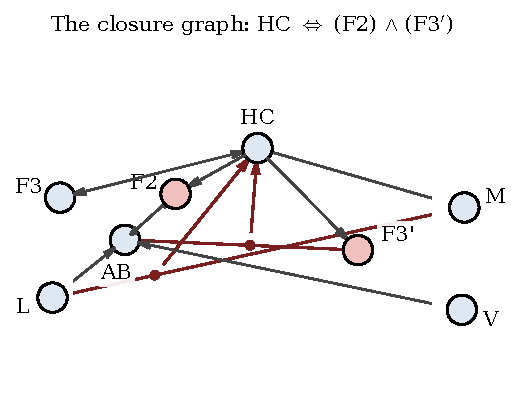
\includegraphics[width=0.92\textwidth]{figures/fig_graph}
\caption{The closure graph of Table~\ref{tab:rules}. Grey arrows are rules with one premise; a red fork joins the two premises of a rule that needs both. The coloured nodes are \Fii{} and \Fiii{}.}
\label{fig:graph}
\end{figure*}

\section{The algebraic locus in a family}\label{sec:loci}

\begin{definition}\label{def:algloc}
Let $\pi\colon\mathcal{X}\to S$ be a smooth projective morphism to a smooth connected complex quasi-projective variety, and let $\xi$ be a global section of $R^{2p}\pi_{*}\QQ$ that is a Hodge class at one point. The algebraic locus of $\xi$ is the set $\Sigma(\xi)$ of $s\in S$ at which $\xi_{s}\in H^{2p}(\mathcal{X}_{s})$ is algebraic.
\end{definition}

By the theorem of the fixed part \cite{Del71,And92}, the flat sections of a polarisable variation form a sub-Hodge structure, constant along $S$; so $\xi_{s}$ is a Hodge class at every point once it is one somewhere.\footnote{The theorem says that for a polarisable variation of Hodge structure $\mathcal{V}$ over a smooth connected quasi-projective base $S$, the space $H^{0}(S,\mathcal{V})$ of global flat sections, which is the subspace of a fibre $\mathcal{V}_{s}$ fixed by the monodromy group, is a sub-Hodge structure of $\mathcal{V}_{s}$, and the Hodge structure it carries does not depend on $s$. Deligne proved it for the variations $R^{k}\pi_{*}\QQ$ of a smooth projective morphism, where it follows from the degeneration of the Leray spectral sequence and the weight filtration of a smooth compactification; Andr\'e proved it for every polarisable variation by showing that the connected monodromy group is a normal subgroup of the derived group of the generic Mumford--Tate group. In the situation of the text the section $\xi$ is flat, so its value at one point is fixed by the monodromy; if that value has type $(p,p)$ at one point, the sub-Hodge structure of flat sections contains it as a Hodge class, and since that Hodge structure is the same at every point, $\xi_{s}$ has type $(p,p)$ everywhere.}

\begin{lemma}[Dichotomy]\label{lem:dichotomy}
\leavevmode
\begin{enumerate}[label=\textup{(\roman*)},leftmargin=2.4em,itemsep=2pt]
\item $\Sigma(\xi)$ is a countable union of Zariski closed subsets of $S$.
\item Either $\Sigma(\xi)=S$ or $\Sigma(\xi)$ is meagre in $S^{\mathrm{an}}$.
\item The following are equivalent: $\Sigma(\xi)=S$; $\Sigma(\xi)$ has an interior point; $\Sigma(\xi)$ is not meagre; $\xi_{s}$ is algebraic for the very general $s$. If $\Sigma(\xi)$ is dense they are equivalent to $\Sigma(\xi)$ being closed.
\end{enumerate}
\end{lemma}

\begin{proof}
(i) Fix a relatively ample line bundle on $\mathcal{X}$. For a Hilbert polynomial $P$ the relative Hilbert scheme $\mathrm{Hilb}^{P}(\mathcal{X}/S)$ is projective over $S$ \cite{Gro61}, and the class of the fibre of the universal family in $H^{2p}(\mathcal{X}_{s})$ is locally constant on each connected component of it, since a flat family of subschemes over a connected base has locally constant cycle class. A rational combination $\sum_{i}a_{i}[Z_{i}]$ equal to $\xi_{s}$ is a point of a fibre product $\prod_{S}\mathrm{Hilb}^{P_{i}}(\mathcal{X}/S)$, projective over $S$ and with countably many connected components; on each component the condition $\sum a_{i}[Z_{i}]=\xi$ is either empty or holds throughout, because both sides are flat sections. So $\Sigma(\xi)$ is the union, over the countably many tuples $(P_{i},a_{i})$ and components, of images of proper morphisms to $S$, each Zariski closed.

(ii) A countable union of proper Zariski closed subsets of an irreducible $S$ has empty interior in $S^{\mathrm{an}}$, and each is closed, so the union is meagre; if one of the closed sets is $S$ itself, $\Sigma(\xi)=S$.

(iii) By the Baire category theorem\footnote{A subset of a topological space is meagre when it is a countable union of nowhere dense sets, that is, of sets whose closure has empty interior. The Baire category theorem states that a complete metric space, or a locally compact Hausdorff space, is not meagre in itself; a connected complex manifold such as $S^{\mathrm{an}}$ is locally compact, so the theorem applies to it. A proper Zariski closed subset of an irreducible variety has empty interior in the analytic topology, because a holomorphic function vanishing on an open set vanishes identically on a connected manifold; so a countable union of proper Zariski closed subsets is meagre, and the alternative in (ii) is exactly whether one of the countably many closed strata of (i) is the whole of $S$.} $S^{\mathrm{an}}$ is not meagre in itself, so $\Sigma(\xi)=S$ excludes meagreness, and a set with an interior point is not meagre; by (ii) not meagre forces $\Sigma(\xi)=S$. The complement of a countable union of proper closed subvarieties is the very general locus, so algebraicity at the very general point means that one of the closed sets is all of $S$. A dense set that is also closed is $S$.
\end{proof}

\begin{lemma}[Points of CM type are dense]\label{lem:cmdense}
Let $G$ be a connected reductive group over $\QQ$, $u_{0}\colon U(1)\to G_{\RR}$ a homomorphism and $\cD$ the orbit of $u_{0}$ under conjugation by $G(\RR)^{+}$. The points $u\in\cD$ for which $u(U(1))$ lies in the real points of a maximal torus of $G$ defined over $\QQ$ are dense in $\cD$.
\end{lemma}

\begin{proof}
Let $u_{1}\in\cD$ and $W$ a neighbourhood of $u_{1}$. A maximal torus $T_{1}$ of $G_{\RR}$ contains $u_{1}(U(1))$, since the centraliser of that compact torus is reductive and connected. Pick a regular element $Y_{1}$ in the Lie algebra $\mathfrak{t}_{1}$ of $T_{1}$. The map $(g,Y)\mapsto\mathrm{Ad}(g)Y$ from $G(\RR)^{+}\times\mathfrak{t}_{1}$ to $\mathfrak{g}_{\RR}$ is submersive at $(1,Y_{1})$ because $\mathfrak{g}_{\RR}=\mathfrak{t}_{1}\oplus[\mathfrak{g}_{\RR},Y_{1}]$, so the image of a small neighbourhood $N_{1}\times N_{2}$, with $N_{1}u_{1}N_{1}^{-1}\subseteq W$ and $N_{2}$ made of regular elements, contains an open set of $\mathfrak{g}_{\RR}$, hence a rational point $Y=\mathrm{Ad}(g)Y'$. The identity component $T$ of the centraliser of the rational regular semisimple $Y$ is a maximal torus over $\QQ$ with $T_{\RR}=gT_{1}g^{-1}$, and $u=gu_{1}g^{-1}\in W$ has $u(U(1))\subseteq T_{\RR}$.
\end{proof}

When $G=\Hg(A)$ and $u$ is the Hodge cocharacter of an abelian variety $A$, the condition of the lemma says that $\Hg(A)$ lies in a $\QQ$-torus, and then $A$ is of CM type: a maximal $\QQ$-torus of $\mathrm{GL}(H^{1}(A))$ containing it is the unit group of a commutative semisimple algebra $L$ of dimension $2\dim A$ commuting with $\Hg(A)$, and the commutant of $\Hg(A)$ is $\End^{0}(A)$.

\begin{proposition}[A family with a CM member through every Hodge class]\label{prop:cmfamily}
Let $A_{0}$ be an abelian variety and $\gamma$ a Hodge class on it. There are a polarised abelian scheme $\pi\colon\cA\to S$ over a smooth connected quasi-projective base, a flat section $\xi$ of $R^{2p}\pi_{*}\QQ$, a point $s_{0}$ with $\cA_{s_{0}}\cong A_{0}$ and $\xi_{s_{0}}=\gamma$, and a point $c$ with $\cA_{c}$ of CM type; the points of CM type are dense in $S$.
\end{proposition}

\begin{proof}
Let $G=\Hg(A_{0})$, let $u_{0}$ be the Hodge cocharacter of $A_{0}$ and $\cD$ its $G(\RR)^{+}$-orbit. Every $u\in\cD$ defines a polarisable Hodge structure of weight one on $H^{1}(A_{0})$ with Hodge group contained in $G$, so an abelian variety $A_{u}$ up to isogeny; fixing the lattice $H^{1}(A_{0},\ZZ)$, the polarisation of $A_{0}$ and a level structure of level $N\ge3$, the quotient $S=\Gamma\backslash\cD$ by a neat congruence subgroup $\Gamma\subseteq G(\QQ)$ is a smooth quasi-projective variety carrying a polarised abelian scheme with these fibres \cite{Mum69,Del71}. The class $\gamma$ is invariant under $G$, so it is a flat section $\xi$ of $R^{2p}\pi_{*}\QQ$, and $\xi_{s_{0}}=\gamma$ at the image $s_{0}$ of $u_{0}$. By Lemma~\ref{lem:cmdense} the points of CM type are dense in $\cD$, hence in $S$.
\end{proof}

\begin{theorem}[\Fii{} is propagation from CM points]\label{thm:propagation}
The following are equivalent.
\begin{enumerate}[label=\textup{(\roman*)},leftmargin=2.4em,itemsep=2pt]
\item \Fii{}.
\item $\AB$.
\item For every polarised abelian scheme $\pi\colon\cA\to S$ and every flat Hodge class $\xi$, algebraicity of $\xi_{s}$ at one point $s$ forces $\Sigma(\xi)=S$.
\item The same for the points $s$ of CM type.
\item For every $\pi$, $\xi$ with $\xi_{c}$ algebraic at a point $c$ of CM type, $\Sigma(\xi)$ has an interior point.
\end{enumerate}
\end{theorem}

\begin{proof}
(i) and (ii) are Theorem~\ref{thm:f2isab}. If (ii) holds, $\xi_{t}$ is a Hodge class at every $t$ by the theorem of the fixed part and algebraic by (ii), so (iii) holds; (iv) is a case of (iii), and (iv) and (v) are equivalent by Lemma~\ref{lem:dichotomy}(iii).

Assume (iv). Let $F$ be a CM field and $n\ge2$. The family of abelian varieties of split Weil type for $F$ over its Shimura variety is a polarised abelian scheme on which the Weil classes are flat sections, and by \cite[Thm.~1.1(i)]{BMB26} they are algebraic at a member isogenous to a product of abelian varieties with complex multiplication by $F$, a member of CM type; so by (iv) they are algebraic on every member, and by pull-back along an $F$-linear isogeny on every abelian variety of split Weil type for $F$. By Andr\'e's theorem \cite{And92cm}, every Hodge class on an abelian variety of CM type is a sum of pull-backs, along homomorphisms, of Weil classes of abelian varieties of split Weil type; so $\AB$ holds for every abelian variety of CM type. Now let $A_{0}$ be any abelian variety and $\gamma$ a Hodge class on it, and take $\pi$, $\xi$, $s_{0}$, $c$ from Proposition~\ref{prop:cmfamily}. Then $\xi_{c}$ is algebraic, (iv) gives $\Sigma(\xi)=S$, and $\gamma=\xi_{s_{0}}$ is algebraic. This is (ii).
\end{proof}

\begin{proposition}[The Weil classes]\label{prop:weil-dense}
For every CM field $F$, every $n\ge2$ and every discriminant, the algebraic locus of the Weil classes in the polarised period domain $\cD_{F}$ contains an explicit point of CM type and is dense, and it is either $\cD_{F}$ or meagre.
\end{proposition}

\begin{proof}
This is \cite[Thm.~1.1]{BMB26}, items (i) to (iii). The density is the Hecke orbit of the base point: the group $G_{F}(\QQ)$ of the unitary group of the hermitian form acts on $\cD_{F}$ through $F$-linear isogenies that preserve the polarisation up to a scalar, hence preserve the algebraicity of the Weil classes, and its closure contains $G_{F}(\RR)^{+}$, which acts transitively. The dichotomy is Lemma~\ref{lem:dichotomy}.
\end{proof}

\begin{proposition}[\Fiii{} and the abelian part]\label{prop:abpart}
Let $H^{2p}_{\mathrm{ab}}(X)\subseteq H^{2p}(X)$ be the sum of the images of all maps $\Gamma_{*}\colon H^{k}(B)\to H^{2p}(X)$ with $B$ abelian and $\Gamma$ an algebraic cycle on $B\times X$. Then $H^{2p}_{\mathrm{ab}}(X)$ is a sub-Hodge structure, $\Ab^{p}(X)=\Hdg^{p}(X)\cap H^{2p}_{\mathrm{ab}}(X)$, and \Fiii{} holds for $X$ in degree $2p$ if and only if a Hodge complement $T^{2p}_{\mathrm{ab}}(X)$ of $H^{2p}_{\mathrm{ab}}(X)$ carries no nonzero Hodge class.
\end{proposition}

\begin{proof}
Each $\Gamma_{*}$ is a morphism of Hodge structures, so its image and the sum of finitely many images, which is all of $H^{2p}_{\mathrm{ab}}(X)$ by dimension, are sub-Hodge structures. A Hodge class in $H^{2p}_{\mathrm{ab}}(X)$ is $\sum\Gamma_{j*}y_{j}$, and the argument of Proposition~\ref{prop:f3prime-known}(i) replaces each $y_{j}$ by a Hodge class; so $\Ab^{p}(X)=\Hdg^{p}(X)\cap H^{2p}_{\mathrm{ab}}(X)$. A Hodge complement exists because the Hodge group is reductive, and the Hodge classes of $H^{2p}(X)$ are the direct sum of those of the two summands, which gives the last assertion.
\end{proof}

Theorem~\ref{thm:intro-loci} is Lemma~\ref{lem:dichotomy}, Theorem~\ref{thm:propagation}, Proposition~\ref{prop:weil-dense} and Proposition~\ref{prop:abpart}. Figure~\ref{fig:locus} draws the locus of Proposition~\ref{prop:weil-dense}.

\begin{figure*}[t]
\centering
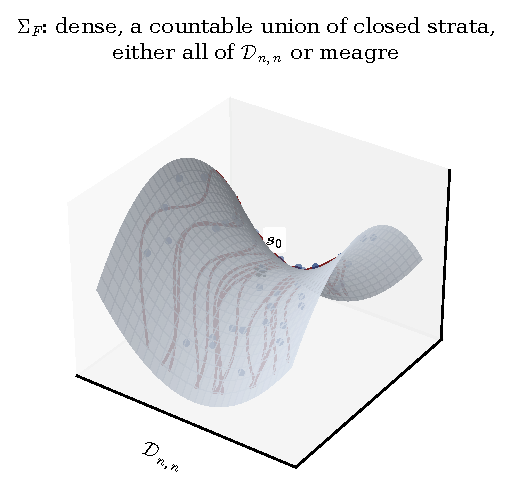
\includegraphics[width=0.92\textwidth]{figures/fig_locus}
\caption{The period domain $\cD_{n,n}$ of a Weil family as a surface. The star is the CM base point, the dots and curves are strata of the algebraic locus, dense by the Hecke orbit. The locus is a countable union of closed strata; it is either the whole surface or meagre.}
\label{fig:locus}
\end{figure*}

Both statements are now of one shape. There is a dense set of points at which the class is algebraic by an explicit cycle; the locus is a countable union of closed strata; the statement is that this union is not meagre, that is, that algebraicity propagates from the dense set. The rest of the paper goes to the first point where the propagation is not known and builds the object that would carry it.

\section{Constructions at \Fiii{}: real multiplication on K3 surfaces}\label{sec:f3prime}

\subsection{Where the first class is}

Let $S$ be a projective K3 surface, $T=T(S)_{\QQ}$ and $E=\End_{\Hdg}T$. The Hodge classes of $S\times S$ are $H^{0}\otimes H^{4}$, $H^{4}\otimes H^{0}$ and $\End_{\Hdg}H^{2}(S)=\End(\NS_{\QQ})\oplus E$, since $T$ is irreducible with no class of type $(1,1)$ and $\Hom_{\Hdg}(T,\NS_{\QQ})=0$. The first two pieces and $\End(\NS_{\QQ})$ are spanned by products of divisor classes. So the Hodge conjecture for $S\times S$ is the algebraicity of $E$, and by Proposition~\ref{prop:abpart} the same classes decide \Fiii{} for $S\times S$ once $T$ is not reached from abelian varieties. When $E$ is a CM field it is spanned by its elements of norm one, which are Hodge isometries of $T$ and algebraic by Buskin's theorem \cite{Bus19}; see \cite[Rem.~2.16]{Var23}. When $E$ is totally real, the Rosati involution is the identity on it \cite{Zar83}, every $e\in E$ is self-adjoint for the intersection form $q$, and $q(ex,ey)=q(e^{2}x,y)$. The first class is a real multiplication.

\subsection{Chains of correspondences}

\begin{lemma}\label{lem:dominant}
Let $f\colon S\dashrightarrow S'$ be a dominant rational map of K3 surfaces of degree $d$ and $\Gamma_{f}$ the closure of its graph. Then $f_{*}=\Gamma_{f*}$ and $f^{*}=\Gamma_{f*}^{t}$ are morphisms of Hodge structures, $f^{*}$ maps $T(S')_{\QQ}$ isomorphically onto $T(S)_{\QQ}$ with $q_{S}(f^{*}a,f^{*}b)=d\,q_{S'}(a,b)$, and $f_{*}=d\,(f^{*})^{-1}$ on $T(S)_{\QQ}$.
\end{lemma}

\begin{proof}
The graph is an algebraic cycle, so both maps are induced by algebraic classes and are morphisms of Hodge structures. Pull-back of a nowhere vanishing $2$-form is a nonzero $2$-form, so $f^{*}(T(S')_{\QQ})$ is a sub-Hodge structure of $H^{2}(S)$ that meets $H^{2,0}(S)$; the smallest sub-Hodge structure of $H^{2}(S)$ containing $H^{2,0}$ is $T(S)_{\QQ}$, so $f^{*}T(S')_{\QQ}\supseteq T(S)_{\QQ}$, and since $T(S')_{\QQ}$ is irreducible and $f^{*}$ is injective on it ($f_{*}f^{*}=d$), equality of dimensions gives $f^{*}T(S')_{\QQ}=T(S)_{\QQ}$. The projection formula gives $q_{S}(f^{*}a,f^{*}b)=q_{S'}(f_{*}f^{*}a,b)=d\,q_{S'}(a,b)$ and $f_{*}f^{*}=d$.
\end{proof}

\begin{lemma}\label{lem:isometry}
A Hodge isometry $\varphi\colon T(S)_{\QQ}\to T(S')_{\QQ}$ is induced by an algebraic class on $S\times S'$.
\end{lemma}

\begin{proof}
The spaces $\NS(S)_{\QQ}$ and $\NS(S')_{\QQ}$ are the orthogonal complements of $T(S)_{\QQ}$ and $T(S')_{\QQ}$ in the two copies of $\Lambda_{\QQ}$, isometric to each other through $\varphi$; by Witt's cancellation theorem the complements are isometric, so $\varphi$ extends to a Hodge isometry $H^{2}(S)\to H^{2}(S')$, which is algebraic by Buskin's theorem \cite{Bus19} (see \cite[Thm.~0.1]{Huy19}). The projector of $H^{2}(S)$ onto $T(S)_{\QQ}$ along $\NS(S)_{\QQ}$ is algebraic, being $1$ minus the projector onto $\NS$, which is a sum $\sum_{i,j}c_{ij}\,D_{i}\otimes D_{j}$ over a basis of divisor classes with $(c_{ij})$ the inverse Gram matrix; composing gives $\varphi$ on $T$ and zero on $\NS$.
\end{proof}

\begin{theorem}[Chains]\label{thm:chain}
Let $S$ be a projective K3 surface with $E$ totally real and $e\in E$ with $e^{2}=n\in\QQ_{>0}$. Suppose there are projective K3 surfaces $S=S_{0},S_{1},\dots,S_{r}$ and, for each $i$, either a dominant rational map $S_{i-1}\dashrightarrow S_{i}$ of degree $n_{i}$, a dominant rational map $S_{i}\dashrightarrow S_{i-1}$ of degree $n_{i}$, or a Hodge isometry $T(S_{i-1})_{\QQ}\cong T(S_{i})_{\QQ}$ (and then $n_{i}=1$), such that
\[
\prod_{i}n_{i}^{\pm1}\equiv n\pmod{\QQ^{\times2}},
\]
the sign being $+$ for maps leaving $S_{i-1}$ and $-$ for maps arriving at it. Then $e$ is algebraic on $S\times S$.
\end{theorem}

\begin{proof}
Composing along the chain the maps $f_{*}$ for maps leaving $S_{i-1}$, $f^{*}$ for maps arriving, and the classes of Lemma~\ref{lem:isometry} for the isometries, gives an algebraic isomorphism $\phi\colon T(S_{r})_{\QQ}\to T(S)_{\QQ}$ of Hodge structures with $q_{S}(\phi a,\phi b)=\mu\,q_{S_{r}}(a,b)$, where $\mu=\prod n_{i}^{\pm1}$ by Lemma~\ref{lem:dominant} (a map leaving contributes $f_{*}=n_{i}(f^{*})^{-1}$, of multiplier $n_{i}$; a map arriving contributes $f^{*}$, of multiplier $n_{i}$ in the other direction, that is $n_{i}^{-1}$ for the composite in the direction of $\phi$). Write $\mu=nc^{2}$ with $c\in\QQ^{\times}$. Since $e$ is self-adjoint with $e^{2}=n$, it is a Hodge similarity of $T(S)_{\QQ}$ of multiplier $n$. So $\psi=(c^{-1}\phi)^{-1}\circ e\colon T(S)_{\QQ}\to T(S_{r})_{\QQ}$ is a Hodge isometry, algebraic by Lemma~\ref{lem:isometry}, and $e=(c^{-1}\phi)\circ\psi$ is a composite of algebraic correspondences, hence algebraic on $S\times S$.
\end{proof}

The case $r=1$ with $S\dashrightarrow S_{1}$ the quotient by a symplectic automorphism of prime order $p$ is Varesco's theorem \cite[Thm.~2.1]{Var23}, which gives $e=\sqrt p$ and is used for $p=2,3$. What a chain adds is a composite multiplier.

\subsection{Real multiplication by \texorpdfstring{$\QQ(\sqrt6)$}{Q(sqrt 6)}}

A symplectic automorphism of finite order on a K3 surface acts trivially on $T(S)$, its quotient has a K3 resolution $Y$ \cite{Nik80b} (for involutions and their quotients see also \cite{BN26}), and $T(Y)_{\QQ}\cong T(S)_{\QQ}(1/\mathrm{ord})$ by Lemma~\ref{lem:dominant}. The invariant lattice of a symplectic involution is $U^{3}\oplus E_{8}(-2)$, and a K3 surface has a symplectic involution exactly when $E_{8}(-2)$ embeds primitively in its N\'eron--Severi lattice \cite{Mor84,vGS07}. The invariant lattice of a symplectic automorphism of order three is $U\oplus U(3)^{2}\oplus A_{2}^{2}$, and such an automorphism exists exactly when the Coxeter--Todd lattice $K_{12}(-2)$ embeds primitively in the N\'eron--Severi lattice \cite[Thm.~4.1]{GS07}. Put
\[
V_{2}=\bigl(U^{3}\oplus E_{8}(-2)\bigr)_{\QQ},\qquad V_{3}=\bigl(U\oplus U(3)^{2}\oplus A_{2}^{2}\bigr)_{\QQ},
\]
of ranks $14$ and $10$ and signatures $(3,11)$ and $(3,7)$; over $\QQ$, $U(3)\cong U$ and $E_{8}(-2)\cong\langle-1\rangle^{8}\cong\langle-2\rangle^{8}$. Varesco \cite[Props.~2.5 and 2.11]{Var23} shows that a projective K3 surface whose transcendental space embeds isometrically in $V_{2}$ (resp.\ $V_{3}$) is Hodge isometric to one with a symplectic involution (resp.\ a symplectic automorphism of order three).

\begin{lemma}[Embedding criterion]\label{lem:embed}
Let $W$ and $V$ be rational quadratic spaces with $\mathrm{rk}\,V-\mathrm{rk}\,W\ge3$. Then $W$ embeds isometrically in $V$ if and only if the signature of $V$ dominates that of $W$ in both signs. In that case a complement $W'$ exists with $V\cong W\oplus W'$.
\end{lemma}

\begin{proof}
Necessity is clear. For sufficiency put $k=\mathrm{rk}\,V-\mathrm{rk}\,W\ge3$ and let $(s_{+},s_{-})$ be the difference of signatures, $s_{+}+s_{-}=k$. A quadratic space $W'$ of rank $k$ and signature $(s_{+},s_{-})$ with prescribed discriminant $d'=d(V)d(W)$ and prescribed Hasse invariants $\varepsilon_{p}'$ exists provided the $\varepsilon'_{p}$ equal $1$ for almost all $p$, $\prod_{p\le\infty}\varepsilon'_{p}=1$, and $\varepsilon'_{\infty}$, $d'$ match the signature \cite[Chap.~IV, Prop.~7]{Ser73}, with no further condition when $k\ge3$. Take $\varepsilon'_{p}=\varepsilon_{p}(V)\varepsilon_{p}(W)(d(W),d')_{p}$, the value forced by the formula $\varepsilon_{p}(W\oplus W')=\varepsilon_{p}(W)\varepsilon_{p}(W')(d(W),d(W'))_{p}$. The product formula for these holds because it holds for $V$, for $W$ and for the Hilbert symbol. Then $W\oplus W'$ and $V$ have the same rank, signature, discriminant and Hasse invariants at every place, so they are isometric by the Hasse--Minkowski theorem \cite[Chap.~IV, Thm.~9]{Ser73}, and $W$ embeds in $V$.
\end{proof}

\begin{theorem}[Two-dimensional families with algebraic real multiplication by $\QQ(\sqrt6)$]\label{thm:sqrt6}
Let $S$ be a projective K3 surface with $\QQ(\sqrt6)\subseteq E$ whose transcendental space $T=T(S)_{\QQ}$ embeds isometrically in $V_{3}$.
\begin{enumerate}[label=\textup{(\roman*)},leftmargin=2.4em,itemsep=2pt]
\item $\sqrt6\in E$ is algebraic on $S\times S$.
\item The Hodge conjecture, and \Fiii{}, hold for $S\times S$ and for the Hilbert square $S^{[2]}$.
\item Such surfaces exist in two-dimensional families, whose very general member has $\mathrm{rk}\,T=8$ and $E=\QQ(\sqrt6)$ exactly. One such family is the one whose transcendental space is $E^{4}$ with the trace form of $q_{E}=\langle-2,-2,-2+\sqrt6,-1+\sqrt6\rangle$ over $E=\QQ(\sqrt6)$.
\end{enumerate}
\end{theorem}

\begin{proof}
(i) By \cite[Prop.~2.11]{Var23} $S$ is Hodge isometric to a K3 surface $S'$ with a symplectic automorphism $\sigma$ of order three, and by Lemma~\ref{lem:isometry} the isometry is algebraic, so we may replace $S$ by $S'$. Let $Y$ be the minimal resolution of $S'/\sigma$ and $f_{1}\colon S'\dashrightarrow Y$ the quotient map, of degree three, so that $T(Y)_{\QQ}\cong T(1/3)$, of rank $\mathrm{rk}\,T\le8$ and signature $(2,\mathrm{rk}\,T-2)$: the rank is at most $8$ because $T$ embeds in $V_{3}$ of rank $10$ and signature $(3,7)$ with a complement that must contain the remaining positive direction, so the complement has rank at least two. Now $T(Y)_{\QQ}$ has rank at most $8$ and signature dominated by $(3,11)$, and $14-8\ge3$, so by Lemma~\ref{lem:embed} it embeds in $V_{2}$. By \cite[Prop.~2.5]{Var23} $Y$ is Hodge isometric to a K3 surface $Y'$ with a symplectic involution $\iota$; let $Z$ be the resolution of $Y'/\iota$ and $f_{2}\colon Y'\dashrightarrow Z$ the quotient, of degree two. The chain $S'\dashrightarrow Y\cong Y'\dashrightarrow Z$ has multiplier $3\cdot1\cdot2=6$, and Theorem~\ref{thm:chain} applies to $e=\sqrt6$ (Fig.~\ref{fig:chain}).

(ii) By the first paragraph of this section it remains to make $E$ algebraic. $E$ contains $\QQ(\sqrt6)$, and either $E=\QQ(\sqrt6)$ or $E$ is a CM field: a totally real $E$ has $\dim_{E}T\ge3$, because the complex line $H^{2,0}$ lies in one eigenspace $T_{\sigma}\otimes\CC$ and $\overline{H^{2,0}}$ in the same one, so that $T_{\sigma}\otimes\RR$ has signature $(2,\ast)$ and $\dim_{E}T\ge3$ follows from $q$ being negative definite on the other eigenspaces together with $T\otimes\RR$ having exactly two positive directions; and $[E:\QQ]\cdot\dim_{E}T=\mathrm{rk}\,T\le8$ then forces $[E:\QQ]\le2$. If $E=\QQ(\sqrt6)$, (i) suffices. If $E$ is CM, it is spanned by its norm-one elements, Hodge isometries, algebraic by Buskin's theorem. So every Hodge class on $S\times S$ is algebraic, and \Fiii{} follows. For $S^{[2]}$ the Chow motive is a direct summand of twists of $h(S\times S)$, $h(S)$ and $\mathbf{1}$ \cite{dCM02}, so every Hodge class on $S^{[2]}$ is the image under an algebraic correspondence of a Hodge class on $S\times S$ or $S$, and both statements follow.

(iii) Let $E=\QQ(\sqrt6)$ with real embeddings $\sigma_{1}$, $\sigma_{2}$ ($\sqrt6\mapsto\pm\sqrt6$), and let $q_{E}=\langle a_{1},a_{2},a_{3},a_{4}\rangle$ with $a_{1},a_{2}$ negative at both places and $a_{3},a_{4}$ positive at $\sigma_{1}$, negative at $\sigma_{2}$. The $\QQ$-space $T=E^{4}$ with the form $\Tr_{E/\QQ}\circ q_{E}$ has rank $8$ and signature $(2,2)+(0,4)=(2,6)$, and multiplication by $\sqrt6$ is self-adjoint of square $6$. For $q_{E}=\langle-2,-2,-2+\sqrt6,-1+\sqrt6\rangle$ one computes $d(T)=10$, $\varepsilon_{2}=1$, $\varepsilon_{3}=-1$, $\varepsilon_{5}=1$ and $\varepsilon_{p}=1$ otherwise, while $V_{3}$ has $d=-1$, $\varepsilon_{2}=1$, $\varepsilon_{3}=-1$, $\varepsilon_{5}=1$; and $T\oplus\langle1,-10\rangle$ has the invariants of $V_{3}$ at every place, so $V_{3}\cong T\oplus\langle1,-10\rangle$ by Hasse--Minkowski, with a complement containing a positive vector (Table~\ref{tab:invariants}; the Hilbert symbols are recomputed in the programs of Appendix~\ref{app:checks}). Embed $V_{3}$ in $\Lambda_{\QQ}$ as the invariant lattice of an order-three symplectic action, with orthogonal complement $K_{12}(-2)$, and let $N\subseteq\Lambda$ be the primitive sublattice with $N_{\QQ}=T^{\perp}$; it contains $K_{12}(-2)$ primitively and a positive class. The Hodge structures of K3 type on $T$ for which $\sqrt6$ is a Hodge endomorphism are the periods $\omega\in\PP(T_{\sigma_{1}}\otimes\CC)$ with $q(\omega)=0$, $q(\omega,\bar\omega)>0$, where $T_{\sigma_{1}}$ is the $\sigma_{1}$-eigenspace, of signature $(2,2)$; this is a domain of dimension two \cite[Prop.~2.3]{Var23}. For each such $\omega$ the surjectivity of the period map gives a K3 surface $S_{\omega}$ with $T(S_{\omega})_{\QQ}\subseteq T$, projective because $N$ contains a positive class, carrying an order-three symplectic automorphism because $K_{12}(-2)\subseteq N$ primitively. For $\omega$ outside a countable union of proper closed analytic subsets, $T(S_{\omega})_{\QQ}=T$ and $E=\QQ(\sqrt6)$, by the argument of \cite[Thm.~22.9]{BMB26}, which needs only $\dim_{E}T\ge3$.
\end{proof}

\begin{table}[t]
\centering
\caption{Rational invariants used in Theorem~\ref{thm:sqrt6}(iii). Hasse invariants are $+1$ at every prime not shown.}
\label{tab:invariants}
\begin{ruledtabular}
\begin{tabular}{lcccccc}
space & rank & signature & $d$ & $\varepsilon_{2}$ & $\varepsilon_{3}$ & $\varepsilon_{5}$ \\
\colrule
$T=\Tr_{E/\QQ}q_{E}$ & 8 & $(2,6)$ & $10$ & $+1$ & $-1$ & $+1$ \\
$\langle1,-10\rangle$ & 2 & $(1,1)$ & $-10$ & $+1$ & $+1$ & $+1$ \\
$T\oplus\langle1,-10\rangle$ & 10 & $(3,7)$ & $-1$ & $+1$ & $-1$ & $+1$ \\
$V_{3}$ & 10 & $(3,7)$ & $-1$ & $+1$ & $-1$ & $+1$ \\
$V_{2}$ & 14 & $(3,11)$ & $-1$ & $-1$ & $+1$ & $+1$ \\
\end{tabular}
\end{ruledtabular}
\end{table}

\begin{figure*}[t]
\centering
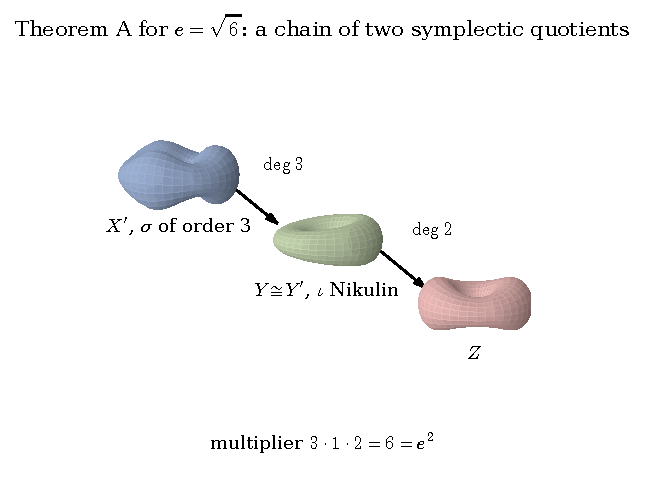
\includegraphics[width=0.84\textwidth]{figures/fig_chain}
\caption{The chain of Theorem~\ref{thm:sqrt6}: the quotient of $S'$ by a symplectic automorphism of order three, a Hodge isometry (algebraic by Buskin), and the quotient of $Y'$ by a Nikulin involution. The multipliers compose to $6$.}
\label{fig:chain}
\end{figure*}

In Varesco's families $E$ is $\QQ(\sqrt2)$ or $\QQ(\sqrt3)$ \cite[Thms.~2.9, 2.15]{Var23}; van Geemen and Sch\"utt obtain $\sqrt2$, $\sqrt3$, $\sqrt7$ from rational self-maps of elliptic K3 surfaces \cite[\S\S6--7]{vGS25}. The lattice condition of Theorem~\ref{thm:sqrt6} is a genuine restriction: among the $165$ sign-admissible diagonal forms $q_{E}$ with small coefficients, $98$ embed in $V_{3}$ and $67$ do not (Appendix~\ref{app:checks}).

\subsection{Isogenies of elliptic surfaces}\label{ssec:fricke}

Varesco's quotients and the chains of Theorem~\ref{thm:chain} produce the square roots of the orders of symplectic automorphisms, $2$ and $3$, and their products. A different source of similarities is a rational self-map of a K3 surface, and the self-maps that exist in families come from isogenies of elliptic fibrations: van Geemen and Sch\"utt obtain $\sqrt2$ and $\sqrt3$ from isogenies of degree $2$ and $3$ in this way, and for degrees $5$ and $7$ they give one surface each \cite[\S\S6--7]{vGS25}. We show that the degrees $5$ and $7$ come in one-dimensional families, that in the families the isogeny is a complex multiplication by $\QQ(\sqrt{-5})$ or $\QQ(\sqrt{-7})$ and not a real one, the sign of its square being decided by how the twisting function behaves under the Fricke involution, and that the families satisfy the Hodge conjecture on all their powers.

Let $N\in\{5,7\}$ and write $N^{k}$ for $125$ when $N=5$ and $49$ when $N=7$. The modular curve $X_{0}(N)$ is rational, with Fricke's coordinate $t$ in which the involution $(E,C)\mapsto(E/C,E[N]/C)$ is $w(t)=N^{k}/t$ \cite[\S7.6]{vGS25}.\footnote{The curve $X_{0}(N)$ parametrises elliptic curves with a cyclic subgroup of order $N$; it has genus zero exactly for $N\le10$ and $N\in\{12,13,16,18,25\}$, and for $N=5$ and $N=7$ a coordinate is the Hauptmodul $t=\bigl(\eta(\tau)/\eta(N\tau)\bigr)^{k}$ with $k=12/(N-1)$, so $k=3$ for $N=5$ and $k=2$ for $N=7$; this is why $N^{k}$ is $125$ in one case and $49$ in the other. The Fricke involution sends $\tau$ to $-1/N\tau$, which exchanges the two cusps $0$ and $\infty$ of $X_{0}(N)$ and, on the moduli interpretation, replaces $(E,C)$ by the quotient $E/C$ with the image of $E[N]$ as its distinguished subgroup. Applying it twice gives $E/E[N]\cong E$, so it is an involution, and in the coordinate $t$ it reads $t\mapsto N^{k}/t$ because $\eta(-1/\tau)=\sqrt{-i\tau}\,\eta(\tau)$ turns the quotient of eta functions into its reciprocal up to the constant $N^{k/2}$, squared to $N^{k}$ by the exponent.} The universal curve with a cyclic subgroup $C_{t}$ of order $N$ over $\PP^{1}_{t}$ is
\begin{equation}\label{eq:fricke}
\mathcal{E}_{t}\colon\ y^{2}=x^{3}-27c_{4}(t)\,x-54c_{6}(t),
\end{equation}
with, for $N=7$,
\begin{align*}
c_{4}&=(t^{2}+13t+49)(t^{2}+5t+1),\\
c_{6}&=(t^{2}+13t+49)(t^{4}+14t^{3}+63t^{2}+70t-7),
\end{align*}
and for $N=5$,
\begin{align*}
c_{4}&=(t^{2}+10t+5)(t^{2}+22t+125),\\
c_{6}&=(t^{2}+4t-1)(t^{2}+22t+125)^{2}.
\end{align*}
The discriminant is $1728\,t\,(t^{2}+13t+49)^{2}$ for $N=7$ and $1728\,t\,(t^{2}+22t+125)^{3}$ for $N=5$, of degree $5$ and $7$. So the relatively minimal model $R_{N}$ of \eqref{eq:fricke} over $\PP^{1}_{t}$ is a rational elliptic surface with fibres of type $\mathrm{I}_{1}$ at $t=0$, $\mathrm{I}_{N}$ at $t=\infty$, and at the two roots $e_{1},e_{2}$ of the quadratic factor, where $c_{4}$ vanishes, of type $\mathrm{II}$ for $N=7$ and $\mathrm{III}$ for $N=5$; the Euler numbers add up to $1+N+2\cdot2=12$ and $1+N+2\cdot3=12$. The roots satisfy $e_{1}e_{2}=N^{k}$, so $w$ exchanges them and exchanges $0$ with $\infty$.

\begin{lemma}[The Fricke isogeny over the function field]\label{lem:fricke}
$\mathcal{E}_{t}/C_{t}\cong\mathcal{E}_{w(t)}$ over $\CC(t)$.
\end{lemma}

\begin{proof}
The two curves have the same $j$-invariant, because $w$ is the Fricke involution of $X_{0}(N)$. Two elliptic curves over $\CC(t)$ with the same non-constant $j$-invariant differ by a quadratic twist $\chi\in\CC(t)^{\times}/\CC(t)^{\times2}$, and a twist ramified at a point of $\PP^{1}$ changes the Kodaira type of the fibre there, exchanging $\mathrm{I}_{n}$ with $\mathrm{I}_{n}^{*}$, $\mathrm{II}$ with $\mathrm{IV}^{*}$ and $\mathrm{III}$ with $\mathrm{III}^{*}$. So it suffices to show that $\mathcal{E}_{t}/C_{t}$ has the same fibre types as $\mathcal{E}_{w(t)}$, which are $\mathrm{I}_{N}$ at $0$, $\mathrm{I}_{1}$ at $\infty$ and $\mathrm{II}$ or $\mathrm{III}$ at $e_{1},e_{2}$: then $\chi$ is unramified on $\PP^{1}$, hence constant, hence trivial over $\CC$.

At $t=0$ the fibre of $\mathcal{E}$ is $\mathrm{I}_{1}$, the Tate curve $\mathbb{G}_{m}/q^{\ZZ}$ over $\CC((t))$, whose only cyclic subgroup of order $N$ rational over $\CC((t))$ is $\mu_{N}$; the quotient $\mathbb{G}_{m}/q^{N\ZZ}$ is $\mathrm{I}_{N}$. At $e_{i}$ the local monodromy $M\in\SL_{2}(\ZZ)$ of $\mathcal{E}$ has order $6$ or $4$ and irreducible characteristic polynomial; the isogeny is given on the period lattices by a matrix $A\in M_{2}(\ZZ)$ with $\det A=N$, and the monodromy of the quotient is $M'=AMA^{-1}$. The $\SL_{2}(\ZZ)$-classes with this characteristic polynomial are those of $M$ and $M^{-1}$, which are the types $\mathrm{II}$ and $\mathrm{II}^{*}$, or $\mathrm{III}$ and $\mathrm{III}^{*}$. If $M'=gM^{-1}g^{-1}$ with $g\in\SL_{2}(\ZZ)$, then $B=g^{-1}A$ conjugates $M$ to $M^{-1}$. All rational matrices doing so form the coset $B_{0}\,\QQ(M)^{\times}$, where $B_{0}=\bigl(\begin{smallmatrix}0&1\\1&0\end{smallmatrix}\bigr)$ for $M=\bigl(\begin{smallmatrix}0&-1\\1&\mathrm{tr}M\end{smallmatrix}\bigr)$ has determinant $-1$ and the elements of the imaginary quadratic field $\QQ(M)$ have positive norm; so $\det B<0$, against $\det B=N$. Hence the quotient has the type of $M$ at $e_{1},e_{2}$. At $\infty$ the $j$-invariant of the quotient has a simple pole, so the fibre is $\mathrm{I}_{1}$ or $\mathrm{I}_{1}^{*}$, and the Euler numbers of the other fibres add up to $11$; since the total is $12$ the fibre is $\mathrm{I}_{1}$.
\end{proof}

For $p\ne q$ in $\PP^{1}_{t}$ let $u_{p,q}=(t-p)(t-q)$, and let $X_{p,q}$ be the elliptic K3 surface whose generic fibre is the quadratic twist $\mathcal{E}_{t}\otimes u_{p,q}$: the twist multiplies $c_{4}$ by $u^{2}$ and $c_{6}$ by $u^{3}$, giving Weierstrass coefficients of degrees $8$ and $12$, and adds two fibres of type $\mathrm{I}_{0}^{*}$ at $p$ and $q$ when these are not among $0,\infty,e_{1},e_{2}$, by Tate's algorithm; the same bookkeeping of Weierstrass coefficients, fibre types and their resolutions in higher dimension is carried out in \cite{Bha26b}. For a double cover $\psi\colon\PP^{1}_{s}\to\PP^{1}_{t}$ let $X_{\psi}$ be the relatively minimal model of $\psi^{*}\mathcal{E}$.

\begin{lemma}\label{lem:twists}
\leavevmode
\begin{enumerate}[label=\textup{(\roman*)},leftmargin=2.4em,itemsep=2pt]
\item $X_{p,q}$ has Picard number at least $16$: its Néron--Severi lattice contains $U\oplus A_{6}\oplus D_{4}^{2}$ for $N=7$ and $U\oplus A_{4}\oplus A_{1}^{2}\oplus D_{4}^{2}$ for $N=5$. The same bound holds for $X_{\psi}$, whose fibres $2\,\mathrm{I}_{1}+2\,\mathrm{I}_{N}$, together with four fibres of type $\mathrm{III}$ when $N=5$, and the pulled-back Mordell--Weil group of $R_{N}$, of rank $2$, give rank at least $16$ by the Shioda--Tate formula.
\item The fibrewise isogeny by $C_{t}$ is a dominant rational map of degree $N$
\[
f\colon X_{p,q}\dashrightarrow X_{w(p),w(q)},\qquad f\colon X_{\psi}\dashrightarrow X_{w\circ\psi}.
\]
\item The deck involution of $\psi$ times $[-1]$ on the fibres is a symplectic involution $\iota$ of $X_{\psi}$, and the minimal resolution of $X_{\psi}/\iota$ is $X_{p,q}$ with $\{p,q\}$ the branch locus of $\psi$. Hence $T(X_{\psi})_{\QQ}\cong T(X_{p,q})_{\QQ}(1/2)$ as in Lemma~\ref{lem:dominant}, and the two surfaces have the same Picard number.
\end{enumerate}
\end{lemma}

\begin{proof}
(i) Shioda--Tate with the fibres listed, and for $X_{\psi}$ the Mordell--Weil rank $8-6=2$ of $R_{N}$. (ii) By Lemma~\ref{lem:fricke} the quotient of the generic fibre is $\mathcal{E}_{w(t)}\otimes u_{p,q}(t)$, and
\begin{widetext}
\begin{equation}\label{eq:frickeu}
u_{p,q}(w(t))=\Bigl(\frac{N^{k}}{t}-p\Bigr)\Bigl(\frac{N^{k}}{t}-q\Bigr)=\frac{pq}{t^{2}}\,u_{w(p),w(q)}(t),
\end{equation}
\end{widetext}
a constant times a square times $u_{w(p),w(q)}$. So $\mathcal{E}_{w(t)}\otimes u_{p,q}(t)\cong\mathcal{E}_{w(t)}\otimes u_{w(p),w(q)}(w(t))$, which is the pull-back along the automorphism $w$ of the base of the generic fibre of $X_{w(p),w(q)}$; pulling back along an automorphism of the base gives an isomorphic surface. For $X_{\psi}$, $(\psi^{*}\mathcal{E})/C=\psi^{*}(\mathcal{E}/C)\cong\psi^{*}w^{*}\mathcal{E}$. (iii) The quadratic twist by the function defining the double cover is the quotient of the base change by the deck involution composed with $[-1]$ on the fibres; the involution is symplectic with eight fixed points, the $2$-torsion of the two fibres over the ramification points, and the quotient's resolution is the twist.
\end{proof}

\begin{lemma}[The sign of the Fricke isogeny]\label{lem:frickesign}
Let $\varphi_{t}\colon\mathcal{E}_{t}\to\mathcal{E}_{w(t)}$ be an isogeny over $\CC(t)$ with kernel $C_{t}$, which exists by Lemma~\ref{lem:fricke} and is unique up to sign, and let $\varphi_{t}^{*}(dx/y)=\lambda(t)\,dx/y$ in the models \eqref{eq:fricke}.
\begin{enumerate}[label=\textup{(\roman*)},leftmargin=2.4em,itemsep=2pt]
\item $\varphi_{w(t)}\circ\varphi_{t}=[-N]$ on $\mathcal{E}_{t}$, and $\lambda(t)\lambda(w(t))=-N$.
\item Let $u\in\CC(t)$ satisfy $u(w(t))=c(t)^{2}u(t)$ with $c\in\CC(t)$, let $X$ be the elliptic K3 surface with generic fibre $\mathcal{E}_{t}\otimes u$, and let $f\colon X\dashrightarrow X$ be the fibrewise isogeny by $C_{t}$ followed by the isomorphism $(x,y)\mapsto(c^{2}x,c^{3}y)$ from $\mathcal{E}_{w(t)}\otimes u(t)$ to $\mathcal{E}_{w(t)}\otimes u(w(t))$, the fibre of $X$ over $w(t)$. Then $f^{*}$ acts on $H^{2,0}(X)$ by a constant $\Lambda$ with
\[
\Lambda^{2}=-\frac{N}{c(t)\,c(w(t))}.
\]
For $u=(t-p)(t-N^{k}/p)$ one has $c(t)c(w(t))=1$ and $\Lambda^{2}=-N$; for $u=t^{2}-N^{k}$ one has $c(t)c(w(t))=-1$ and $\Lambda^{2}=N$.
\end{enumerate}
\end{lemma}

\begin{proof}
(i) The composite is an endomorphism of $\mathcal{E}_{t}$ over $\CC(t)$ of degree $N^{2}$. Since $j$ is not constant, $\End_{\CC(t)}(\mathcal{E}_{t})=\ZZ$, so the composite is $[N]$ or $[-N]$, and changing $\varphi$ to $-\varphi$ does not change it. We read off the sign on the upper half plane $\mathfrak{H}$. Let $\tau\mapsto t(\tau)$ be the quotient map $\mathfrak{H}\to X_{0}(N)$. By the moduli interpretation of $X_{0}(N)$ the pair $(\mathcal{E}_{t(\tau)},C_{t(\tau)})$ is $(\CC/(\ZZ\tau+\ZZ),\langle1/N\rangle)$, analytically in $\tau$, and the Fricke involution lifts to $\tau\mapsto w(\tau)=-1/N\tau$. The map $f_{\tau}(z)=z/\tau$ carries $\ZZ\tau+\ZZ$ into $\ZZ w(\tau)+\ZZ=\ZZ/N\tau+\ZZ$, so it is an isogeny $\CC/(\ZZ\tau+\ZZ)\to\CC/(\ZZ w(\tau)+\ZZ)$, and its kernel $\tau(\ZZ w(\tau)+\ZZ)/(\ZZ\tau+\ZZ)=(\ZZ/N+\ZZ\tau)/(\ZZ\tau+\ZZ)$ is $\langle1/N\rangle$. Its composite with the map of the same form at $w(\tau)$ is $f_{w(\tau)}(f_{\tau}(z))=z/\tau w(\tau)=-Nz$. On the set $\mathfrak{H}'$ of $\tau$ with $j(\tau)\notin\{0,1728\}$ the automorphisms of $\mathcal{E}_{\tau}$ are $\pm1$, so $\varphi_{t(\tau)}=\varepsilon(\tau)f_{\tau}$ with $\varepsilon(\tau)\in\{\pm1\}$; $\varepsilon$ is continuous because $\varphi$ is, hence constant on $\mathfrak{H}'$, which is $\mathfrak{H}$ minus a discrete set and connected. So $\varphi_{w(t)}\circ\varphi_{t}=\varepsilon^{2}f_{w(\tau)}\circ f_{\tau}=[-N]$ on $\mathfrak{H}'$, hence identically. Pulling back $dx/y$ along the composite gives $\lambda(t)\lambda(w(t))\,dx/y$ on one side and $-N\,dx/y$ on the other.

(ii) Over $\CC(t)(\sqrt u)$ the twist by $u$ is the same change of coordinates $(x,y)\mapsto(ux,u^{3/2}y)$ on $\mathcal{E}_{t}$ and on $\mathcal{E}_{w(t)}$, which multiplies $dx/y$ by $u^{-1/2}$ on both, so the twisted isogeny pulls $dx/y$ back to $\lambda(t)\,dx/y$. The isomorphism $(x,y)\mapsto(c^{2}x,c^{3}y)$ pulls $dx/y$ back to $c(t)^{-1}dx/y$, and the holomorphic two-form of $X$, which is $dx/y\wedge dt$ on the Weierstrass model, restricts to the fibre over $w(t)$ as $dx/y\wedge d(w(t))=w'(t)\,dx/y\wedge dt$. Hence $f^{*}(dx/y\wedge dt)=\Lambda(t)\,dx/y\wedge dt$ with $\Lambda(t)=w'(t)\lambda(t)/c(t)$. The pull-back of a holomorphic two-form along a dominant rational map of K3 surfaces is holomorphic off the finitely many points of indeterminacy, hence everywhere, so $f^{*}$ preserves the line $H^{2,0}(X)$ and $\Lambda$ is a constant. Then $\Lambda^{2}=\Lambda(t)\Lambda(w(t))=w'(t)w'(w(t))\,\lambda(t)\lambda(w(t))/c(t)c(w(t))$, where $w'(t)w'(w(t))=(w\circ w)'(t)=1$ and $\lambda(t)\lambda(w(t))=-N$ by (i). For $u=(t-p)(t-N^{k}/p)$ equation \eqref{eq:frickeu} with $q=N^{k}/p$ gives $u(w(t))=(N^{k}/t^{2})\,u(t)$, so $c(t)=N^{k/2}/t$ for a fixed square root $N^{k/2}$, and $c(t)c(w(t))=N^{k}/t\,w(t)=1$. For $u=t^{2}-N^{k}$, $u(w(t))=N^{2k}/t^{2}-N^{k}=-(N^{k}/t^{2})\,u(t)$, so $c(t)=iN^{k/2}/t$ and $c(t)c(w(t))=-1$.
\end{proof}

The archive \cite{BB26code} computes $\lambda$ itself: the kernel polynomial of $\varphi_{t}$ is the factor of degree $(N-1)/2$ of the $N$-th division polynomial over $\ZZ[t,x]$, V\'elu's formulas give the quotient curve, and the isomorphism to \eqref{eq:fricke} at $w(t)$ has $\lambda(t)^{2}=-t^{2}/25$ for $N=5$ and $-t^{2}/7$ for $N=7$, so that $\lambda(t)^{2}\lambda(w(t))^{2}=N^{2}$ and $\Lambda^{2}=-N$ on the pair twists directly; the program \path{code/fricke_sign.py} carries this out, and the Lean file checks the polynomial identity it reduces to.

\begin{theorem}[Fricke families]\label{thm:fricke}
Let $N\in\{5,7\}$ and $K=\QQ(\sqrt{-N})$. Let $\mathfrak{A}_{N}$ be the family of surfaces $X_{p}=X_{p,N^{k}/p}$ for $p\notin\{0,\infty,e_{1},e_{2},\pm\sqrt{N^{k}}\}$, and $\mathfrak{B}_{N}$ the family of surfaces $X_{\psi}$ with $\psi$ branched over a pair $\{b,N^{k}/b\}$.
\begin{enumerate}[label=\textup{(\roman*)},leftmargin=2.4em,itemsep=2pt]
\item Every member $X$ has a dominant rational self-map $f$ of degree $N$ with $f^{*}\in E=\End_{\Hdg}T(X)_{\QQ}$, $f^{*}f_{*}=N$, $(f^{*})^{2}=-N$ and $f_{*}=-f^{*}$. So $K\subseteq E$, with $\sqrt{-N}=\pm f^{*}$ algebraic on $X\times X$, and $E$ is a CM field.
\item The families are not isotrivial, and every member has $\mathrm{rk}\,T(X)\in\{2,4,6\}$. At all but countably many members $E=K$ and the Hodge group of $T(X)$ is the unitary group of the $K$-hermitian form $h$ on $T(X)$ with $\Tr_{K/\QQ}h=q_{X}$; at the others $T(X)$ is of CM type.
\item For every member $X$ and every $n\ge1$ the Hodge conjecture holds for $X^{n}$ and for the Hilbert scheme $X^{[n]}$, and \Fiii{} holds there.
\end{enumerate}
\end{theorem}

Van Geemen and Sch\"utt state that the Fricke parametrisations give one-dimensional families with complex multiplication by $\QQ(\sqrt{-5})$ and $\QQ(\sqrt{-7})$, and give the details for the two surfaces at the fixed points of $w$ only \cite[\S7.6]{vGS25}; (i) and (ii) make their statement explicit, and (iii) is what the complex multiplication gives.

\begin{proof}
(i) $w$ exchanges $p$ and $N^{k}/p$, so Lemma~\ref{lem:twists}(ii) gives $f\colon X_{p}\dashrightarrow X_{p}$, the map of Lemma~\ref{lem:frickesign}(ii) for $u=(t-p)(t-N^{k}/p)$; for $\mathfrak{B}_{N}$, $w\circ\psi$ has the same branch locus as $\psi$, so $w\circ\psi=\psi\circ\sigma$ for a M\"obius transformation $\sigma$ and $X_{w\circ\psi}\cong X_{\psi}$. The correspondence of a dominant rational map preserves $\NS$ and its transpose does too, so it preserves $T=\NS^{\perp}$ and acts there as a morphism of Hodge structures, nonzero since $f^{*}\omega=\Lambda\omega$ with $\Lambda\ne0$; on a resolution $S$ of the graph with $p_{1}\colon S\to X$ birational and $p_{2}$ of degree $N$, both $p_{1}^{*}T$ and $p_{2}^{*}T$ are irreducible sub-Hodge structures of $H^{2}(S)$ containing its unique $(2,0)$-line, so they coincide, and $f_{*}f^{*}=p_{2*}p_{1}^{*}p_{1*}p_{2}^{*}=N$ on $T$. The field $E$ acts faithfully on the line $H^{2,0}(X)$, and $f^{*}$ acts there by $\Lambda$ with $\Lambda^{2}=-N$ by Lemma~\ref{lem:frickesign}(ii); so $(f^{*})^{2}=-N$ in $E$, and $f_{*}=N(f^{*})^{-1}=-f^{*}$. For $X_{\psi}$ the generic fibre is $\mathcal{E}_{\psi(s)}$ over $\CC(s)$, $f$ is the fibrewise isogeny over $\sigma$, and $\sigma$ is an involution: in the coordinate $s$ with $s^{2}=(t-b)/(t-N^{k}/b)$ one computes $(w(t)-b)/(w(t)-N^{k}/b)=b^{2}/N^{k}s^{2}$, so $\sigma(s)=\kappa/s$ with $\kappa^{2}=b^{2}/N^{k}$; the argument of Lemma~\ref{lem:frickesign}(ii) with $c=1$ and $\sigma$ in place of $w$ gives $\Lambda^{2}=\lambda(t)\lambda(w(t))\,\sigma'(s)\sigma'(\sigma(s))=-N$. The adjoint of $f^{*}$ for $q_{X}$ is $f_{*}=-f^{*}$, so the involution of $E$ induced by $q_{X}$ is not the identity; by Zarhin's theorem $E$ is totally real or a CM field \cite[Thm.~1.5.1]{Zar83}, so it is a CM field, and $K=\QQ+\QQ f^{*}\subseteq E$. The class of the graph of $f$ is algebraic, its action on $H^{2}(X)$ is $f^{*}$ on $T$ and an endomorphism of $\NS(X)_{\QQ}$, which is a sum of algebraic classes of $\NS\otimes\NS$; so $f^{*}$, extended by zero on $\NS$, is an algebraic class on $X\times X$.

(ii) The elliptic fibration of $X_{p}$ has labelled singular fibres $\mathrm{I}_{1}$ at $0$, $\mathrm{I}_{N}$ at $\infty$, $\mathrm{II}$ or $\mathrm{III}$ at $e_{1},e_{2}$ and $\mathrm{I}_{0}^{*}$ at $p$ and $N^{k}/p$. An isomorphism of elliptic fibrations induces a M\"obius transformation preserving this configuration; the transformations preserving $\{0,\infty\}$ and $\{e_{1},e_{2}\}$ are $t\mapsto\lambda t$ and $t\mapsto\lambda/t$ with $\lambda e_{1}\in\{e_{1},e_{2}\}$, and since $e_{1}+e_{2}\ne0$ and $e_{1}^{2}\ne e_{2}^{2}$ they are the identity and $w$, which preserve $\{p,N^{k}/p\}$. So $X_{p}$ and $X_{p'}$ have isomorphic fibrations only when $p'\in\{p,N^{k}/p\}$. A K3 surface has finitely many elliptic fibrations up to automorphisms \cite{Ste85}, so the map $p\mapsto[X_{p}]$ to the moduli space has finite fibres and the family is not isotrivial; by local Torelli its period map has uncountable image. By (i) $T(X)_{\QQ}$ is a $K$-vector space, so its rank is even, and it is at most $6$ by Lemma~\ref{lem:twists}(i). It is also an $E$-vector space, so $[E:\QQ]$ divides $\mathrm{rk}\,T(X)$; if $E\ne K$ then $[E:\QQ]\in\{4,6\}$, $\dim_{E}T(X)=1$ and $T(X)$ is of CM type. A Hodge structure of CM type on a sublattice of $M^{\perp}$ is determined by its endomorphism field, a subfield of the endomorphism algebra of the sublattice, and by an eigenline of that field, so the periods of such members form a countable subset of the period domain of $M^{\perp}$; the period map of the family is a non-constant holomorphic map from a connected curve, its fibres over a countable set are countable, so all but countably many members have $E=K$. There the Hodge group of $T(X)$ is the unitary group of the $K$-hermitian form $h$ with $\Tr_{K/\QQ}h=q_{X}$ by Zarhin's theorem for CM fields \cite[Thm.~2.3.1]{Zar83}. The same holds for $\mathfrak{B}_{N}$ by Lemma~\ref{lem:twists}(iii).

(iii) By (i) $E$ is a CM field containing $K$. If $E=K$ then $E=\QQ+\QQ f^{*}$ is algebraic. Otherwise every element of $E$ of norm one to its maximal real subfield is a Hodge isometry of $T$, extended by the identity on $\NS$ to a Hodge isometry of $H^{2}(X,\QQ)$, algebraic by Buskin's theorem \cite{Bus19}. The algebraic classes form a $\QQ$-subalgebra $E'\subseteq E$ containing these elements; for $x\in E$ with $\bar x\ne x$ and $t_{1}\ne t_{2}$ in $\QQ$ it contains $u_i=(t_i+x)/(t_i+\bar x)$ and hence $(u_i-1)^{-1}$. Indeed a finite-dimensional subalgebra of a field is itself a field. The identity
\[
 (u_2-1)^{-1}-(u_1-1)^{-1}=\frac{t_2-t_1}{x-\bar x}
\]
recovers $x-\bar x$, and then $\bar x=(x-\bar x)/(u_1-1)-t_1$. Thus every nonreal $x\in E$ lies in $E'$. Adding a fixed nonreal element also recovers every real element, so $E'=E$. In both cases $\End_{\Hdg}H^{2}(X)=\End(\NS)\oplus E$ is algebraic, and $\Hdg^{2}(X\times X)=\End_{\Hdg}H^{2}(X)\oplus H^{0}\otimes H^{4}\oplus H^{4}\otimes H^{0}$ since $H^{1}=H^{3}=0$, so the Hodge conjecture holds for $X\times X$. For a K3 surface whose endomorphism field is a CM field the Hodge classes in the tensor algebra of $T$ are generated by those of $T\otimes T$, and the Hodge conjecture holds for every power \cite[Thm.~2.2, Cor.~2.3]{Var25}, \cite[Prop.~5.2, Thm.~5.4]{RM08}. It passes to the Hilbert schemes $X^{[n]}$, whose motives are direct summands of motives of powers of $X$ \cite{dCM02}, and \Fiii{} on a variety follows from the Hodge conjecture on it.
\end{proof}

\begin{figure*}[t]
\centering
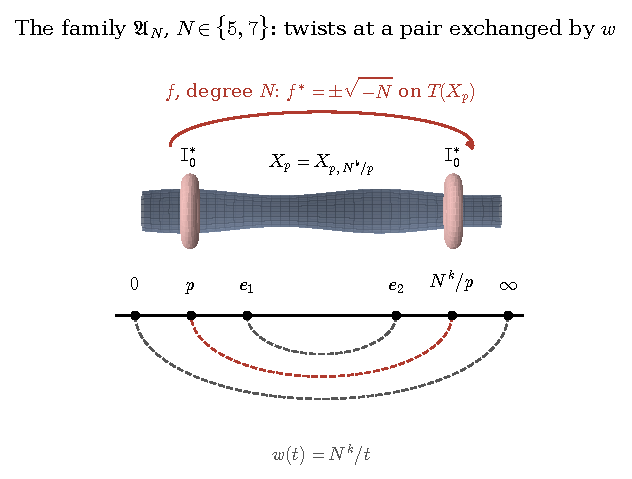
\includegraphics[width=0.92\textwidth]{figures/fig_fricke}
\caption{The family $\mathfrak{A}_{N}$ of Theorem~\ref{thm:fricke}. Over the Fricke coordinate $t$ of $X_{0}(N)$ the involution $w(t)=N^{k}/t$ exchanges the cusps $0$, $\infty$ and the elliptic points $e_{1}$, $e_{2}$; the twist $X_{p}$ at a pair $\{p,N^{k}/p\}$ exchanged by $w$ is carried to itself by the fibrewise isogeny $f$ of degree $N$, and $f^{*}$ is the complex multiplication by $\sqrt{-N}$ on the transcendental lattice.}
\label{fig:fricke}
\end{figure*}

The surface of \cite[\S7.6]{vGS25} with real multiplication by $\sqrt7$ is the twist at $\{7,-7\}$, the two fixed points of $w$, and the surface of \cite[Prop.~7.7]{vGS25} is the twist at the fixed points $\pm5\sqrt5$ for $N=5$, which has Picard number $18$ and complex multiplication as well: there $u=t^{2}-N^{k}$, $c(t)c(w(t))=-1$ and $\Lambda^{2}=N$ by Lemma~\ref{lem:frickesign}(ii), so $f^{*}$ is the real multiplication by $\sqrt N$. The families $\mathfrak{A}_{N}$ are the twists at the pairs exchanged by $w$, where $c(t)c(w(t))=1$ and $\Lambda^{2}=-N$; the two signs are the two values of the constant by which the twisting function changes under $w$ once the square factor $N^{k}/t^{2}$ is removed. The chains of Theorem~\ref{thm:chain} apply to every member, and a member whose field $E$ contained $\sqrt2$, $\sqrt3$ or $\sqrt6$ would have that element algebraic as well; by Theorem~\ref{thm:fricke}(ii) such a member is of CM type, and we know none.

\begin{remark}[The Picard number]\label{rem:frickepicard}
Theorem~\ref{thm:fricke} does not say which of the three ranks the very general member has. The archive decides it by counting points. The surface $X_{1}$, the twist at $\{1,N^{k}\}$, has a Weierstrass model over $\ZZ$ with good reduction at $\ell=11$ for $N=7$ and at $\ell=7$ for $N=5$, primes split in $K$; the program \path{code/fricke_picard.py} counts its points over $\mathbb{F}_{\ell^{i}}$, $i\le3$, fibre by fibre, subtracts the trace of Frobenius on the trivial lattice, and completes the characteristic polynomial of Frobenius on the rank-six complement of the trivial lattice by the functional equation, whose sign is fixed by the nonzero middle coefficient. The polynomials are $x^{6}-726x^{3}+11^{6}$ for $N=7$ and $x^{6}+6x^{5}+56x^{4}+392x^{3}+2744x^{2}+14406x+7^{6}$ for $N=5$; in the variable $x/\ell$ neither has a root of unity among its roots, each is irreducible over $\QQ$ and splits over $K$ into a cubic and its conjugate, as the action of $f^{*}$ requires. By the Tate conjecture for K3 surfaces over finite fields, used in the same way in \cite[\S7]{vGS25}, $\rho(X_{1})=16$, so the very general member of $\mathfrak{A}_{N}$ and of $\mathfrak{B}_{N}$ has $\rho=16$, $\mathrm{rk}\,T=6$, $E=K$ with $\dim_{K}T=3$, and its Hodge group is the unitary group of a hermitian form of signature $(1,2)$ on $K^{3}$. At the primes inert in $K$, $\ell=5$ for $N=7$ and $\ell=11$ for $N=5$, the odd traces vanish, as they must when Frobenius exchanges the two eigenspaces of $f^{*}$. No statement of this section rests on this computation.
\end{remark}

\subsection{The reach of similarities}

Every correspondence used so far acts on transcendental spaces as a Hodge similarity. The next proposition says that this is not an accident of the examples but a property of every correspondence whose components are small, and it measures what a correspondence must look like to act otherwise.

\begin{proposition}[Structure of the transcendental action]\label{prop:structure}
Let $X$, $X'$ be projective K3 surfaces, $\Gamma\in\mathrm{CH}^{2}(X\times X')_{\QQ}$, and $\gamma_{T}\colon T(X)_{\QQ}\to T(X')_{\QQ}$ the map induced on transcendental spaces by composing the action of $\Gamma$ with the orthogonal projections.
\begin{enumerate}[label=\textup{(\roman*)},leftmargin=2.4em,itemsep=2pt]
\item $\gamma_{T}$ is zero or an isomorphism of Hodge structures.
\item If $\gamma_{T}\ne0$ then $a=\gamma_{T}^{\dagger}\gamma_{T}$ lies in the maximal totally real subfield of $E=\End_{\Hdg}T(X)_{\QQ}$ and is totally positive, and $\gamma_{T}$ is a similarity exactly when $a\in\QQ$.
\item Let $\Gamma$ be irreducible, $S$ a resolution of its normalisation with projections $p_{1},p_{2}$ of degrees $d_{1},d_{2}$ to $X$, $X'$. If $p_{1}^{*}T(X)_{\QQ}=p_{2}^{*}T(X')_{\QQ}$ inside $H^{2}(S,\QQ)$, then $\gamma_{T}$ is a similarity of multiplier $d_{1}d_{2}$. This holds whenever $p_{g}(S)\le1$.
\item If $\Gamma$ is irreducible and $\gamma_{T}$ is not a similarity, then $p_{1}^{*}T(X)_{\QQ}\cap p_{2}^{*}T(X')_{\QQ}=0$, so $p_{g}(S)\ge2$ and the transcendental rank of $S$ is at least twice that of $X$.
\item Assume in addition that $E$ is totally real. The $\QQ$-algebra generated by the actions on $T(X)_{\QQ}$ of all correspondences from $X$ to itself whose irreducible components either fail to dominate a factor or have $p_{g}\le1$ is the multiquadratic subfield $E_{2}\subseteq E$ generated by the square roots of the products $d_{1}d_{2}$ that occur. When $[E:\QQ]$ is odd it is $\QQ$.
\end{enumerate}
\end{proposition}

\begin{proof}
(i) $T(X)_{\QQ}$ is an irreducible Hodge structure \cite{Zar83}, and the image of $\gamma_{T}$ is a sub-Hodge structure of $H^{2}(X')$; if nonzero it contains the $(2,0)$-part, hence $T(X')_{\QQ}$, and $\gamma_{T}$ is injective by irreducibility. (ii) $a$ is a Hodge endomorphism of $T(X)$, so $a\in E$, and it is self-adjoint, so it lies in the fixed field of the adjoint involution, the maximal totally real subfield. The form $q'(\gamma x,\gamma y)=q(x,ay)$ is a polarisation of the Hodge structure $T(X)$ up to sign on each real eigenspace of $E$, and comparison with $q$ gives $\sigma(a)>0$ at every real place. A similarity of multiplier $\mu$ has $a=\mu$. (iii) Both $p_{i}^{*}T$ are irreducible sub-Hodge structures of $H^{2}(S)$ with a $(2,0)$-part; if $p_{g}(S)\le1$ they share the unique $(2,0)$-line, so they meet and coincide. When they coincide, $\gamma_{T}=p_{2*}p_{1}^{*}=d_{2}(p_{2}^{*})^{-1}p_{1}^{*}$ on $T$, so $p_{2}^{*}\gamma x=d_{2}\,p_{1}^{*}x$; since $q_{S}(p_{1}^{*}x,p_{1}^{*}y)=d_{1}q(x,y)$ and $q_{S}(p_{2}^{*}x',p_{2}^{*}y')=d_{2}q'(x',y')$, this gives $d_{2}\,q'(\gamma x,\gamma y)=q_{S}(p_{2}^{*}\gamma x,p_{2}^{*}\gamma y)=d_{2}^{2}\,q_{S}(p_{1}^{*}x,p_{1}^{*}y)=d_{1}d_{2}^{2}\,q(x,y)$, that is $q'(\gamma x,\gamma y)=d_{1}d_{2}\,q(x,y)$. (iv) If the two subspaces met they would coincide by irreducibility and (iii) would apply; so they are independent, their $(2,0)$-lines are distinct, and their sum has rank $2\,\mathrm{rk}\,T(X)$ inside the transcendental part of $H^{2}(S)$. (v) A component that does not dominate a factor acts through $\NS$ or through $H^{0}$ and $H^{4}$, hence by zero on $T$. The others act by similarities by (iii), a composite of similarities returning to $X$ is an element $\Phi\in E$ with $\Phi^{\dagger}\Phi\in\QQ$, and for totally real $E$ this is $\Phi^{2}\in\QQ$; such elements generate $E_{2}$. The assertion in (v) uses the totally real hypothesis; it is not asserted for a CM endomorphism field. An odd-degree field has $E_{2}=\QQ$.
\end{proof}

The correspondences of Lemmas~\ref{lem:dominant} and \ref{lem:isometry}, the Fourier--Mukai kernels between a K3 surface and its moduli spaces of sheaves, the rational Hodge isometries of hyper-K\"ahler varieties of K3$^{[n]}$ type \cite{Mar24}, the Fricke isogenies of Theorem~\ref{thm:fricke} and all their composites fall under (iii) or (v). A correspondence that realises an element of a cubic field must therefore have a component whose resolution has $p_{g}\ge2$ and transcendental rank at least twice that of the surface. Such correspondences exist, and the only ones we know come from finite groups.

\begin{proposition}[Hecke correspondences]\label{prop:hecke}
Let $Z$ be a smooth projective surface with an action of a finite group $G$, $H\le G$ a subgroup, and $X$ a smooth projective surface with $p_{g}(X)=1$ birational to $Z/H$; write $\pi\colon Z\dashrightarrow X$.
\begin{enumerate}[label=\textup{(\roman*)},leftmargin=2.4em,itemsep=2pt]
\item For $g\in G$ the correspondence $\Gamma_{g}=(\pi\times\pi)_{*}[\text{graph of }g]$ acts on $H^{2}(X,\QQ)$ as the Hecke operator of the double coset $HgH$, and these operators span a $\QQ$-algebra isomorphic to a quotient of $\End_{G}\QQ[G/H]$ acting by Hodge endomorphisms.
\item Exactly one simple factor of this algebra acts nontrivially on $H^{2,0}(X)$; it is a field, it preserves $T(X)_{\QQ}$, and it embeds into $E$ by algebraic correspondences. If $H^{2,0}(Z)^{G}=0$ this factor is not the one on which $G$ acts trivially.
\item Every field obtained in this way is abelian over $\QQ$. In particular a totally real cubic field $F$ whose Galois closure has group $S_{3}$ is realised by no correspondence built from a finite group acting on a cover of $X$.
\end{enumerate}
\end{proposition}

\begin{proof}
(i) Let $\tilde Z\to Z$ be an equivariant resolution and $\pi\colon\tilde Z\to X$ the quotient by $H$ followed by the resolution; then $\pi_{*}\pi^{*}=|H|$ and $\pi_{*}h^{*}=\pi_{*}$ for $h\in H$, so $\Gamma_{g}$ acts as $\pi_{*}g^{*}\pi^{*}=(\pi^{*})^{-1}\circ\sum_{h\in HgH/H}h^{*}\circ\pi^{*}$ on $H^{2}(X,\QQ)=H^{2}(\tilde Z,\QQ)^{H}$, the Hecke operator of $HgH$. The Hecke operators of $(G,H)$ span $\End_{G}\QQ[G/H]$, a semisimple algebra, and the action on $H^{2}(\tilde Z,\QQ)^{H}$ factors through it. (ii) The idempotents of the simple factors are rational combinations of Hecke operators, so they are Hodge endomorphisms of $H^{2}(X)$; they sum to $1$ and act on the line $H^{2,0}(X)$ by $0$ or $1$, so exactly one of them, $e_{V}$, acts as $1$. A simple factor with nonzero image in the commutative ring $\End_{\Hdg}H^{2,0}(X)=\CC$ through a ring homomorphism to a field is commutative, hence a field $\mathcal{H}_{V}$. For $f\in\mathcal{H}_{V}$, $f(T(X)_{\QQ})$ is a sub-Hodge structure of the transcendental part of $H^{2}(X)$; if $f\omega\ne0$ it contains $\omega$, hence $T(X)_{\QQ}$, and if $f\omega=0$ it has no $(2,0)$-part and lies in $\NS\cap T=0$. So $\mathcal{H}_{V}\to\End_{\Hdg}T(X)_{\QQ}=E$ is a homomorphism from a field, injective. The factor on which $G$ acts trivially fixes $H^{2,0}(\tilde Z)^{G}=H^{2,0}(Z/G)$, which is zero by hypothesis, so it is not $\mathcal{H}_{V}$. (iii) The centres of the simple factors of $\End_{G}\QQ[G/H]$ are the character fields $\QQ(\chi_{i})$ of the irreducible constituents of $\QQ[G/H]$, generated by sums of roots of unity, so each lies in $\QQ(\zeta_{|G|})$ and is abelian; a commutative simple factor is its centre. A non-abelian cubic field is not a subfield of an abelian field.
\end{proof}

For the dihedral group $D_{n}$ with $n$ odd, $H=\langle\tau\rangle$ of order two and $Z$ the elliptic surfaces $\tilde{\mathcal{E}}_{a}$ of \cite[\S4.7]{vGS25}, the algebra $\End_{D_{n}}\QQ[D_{n}/H]$ is $\QQ\times\prod_{d\mid n,\,d>1}\QQ(\zeta_{d})^{+}$, and the factor acting on $\omega$ is $\QQ(\zeta_{n})^{+}$; this is the content of \cite[\S4.8]{vGS25}, where the cycle $\Gamma_{1}+\Gamma_{-1}$ induces $\zeta_{n}+\zeta_{n}^{-1}$. The components of these correspondences are birational to $\tilde{\mathcal{E}}_{a}$, which has $p_{g}\ge2$, as Proposition~\ref{prop:structure}(iv) requires.

\begin{corollary}[Squares of the dihedral families]\label{cor:dihedral}
Let $X$ be an elliptic K3 surface of one of the families of \cite[Thm.~1.1]{vGS25}, with real multiplication by $F=\QQ(\zeta_{n})^{+}$ for $n\in\{5,7,9,11\}$, and suppose $E=F$ or $E$ is a CM field; the very general member has $E=F$. Then the Hodge conjecture holds for $X\times X$, and \Fiii{} holds for $X\times X$ and $X^{[2]}$. This covers the cubic fields $\QQ(\zeta_{7})^{+}$ and $\QQ(\zeta_{9})^{+}$ on families of dimensions $3$ and $2$.
\end{corollary}

\begin{proof}
If $E=F$, $E$ is algebraic by Proposition~\ref{prop:hecke}(ii) and \cite[\S4.8]{vGS25}; if $E$ is CM, by Buskin's theorem as in Theorem~\ref{thm:fricke}(iii). The rest is as there.
\end{proof}

\begin{figure*}[t]
\centering
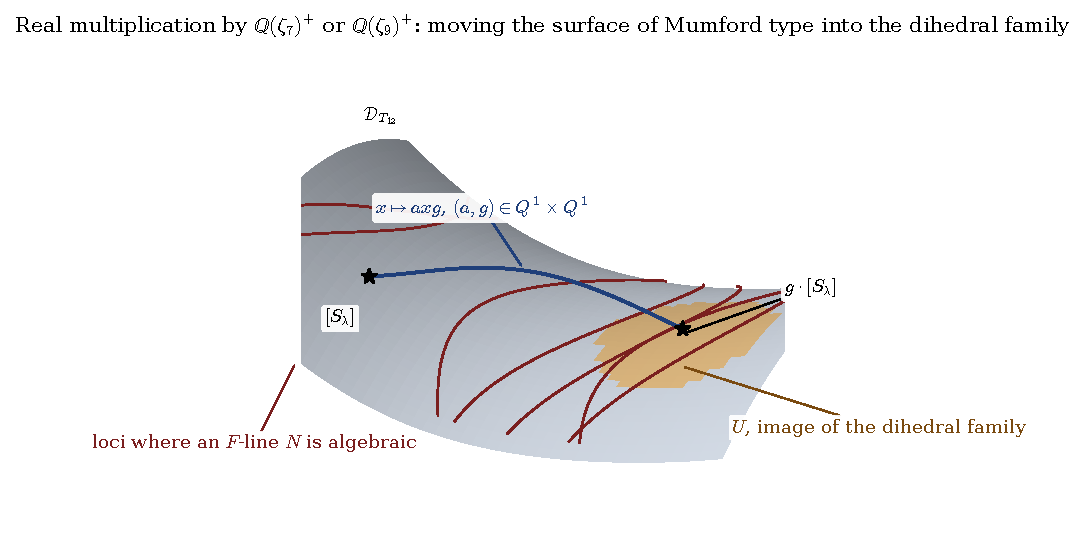
\includegraphics[width=0.92\textwidth]{figures/fig_zeta9}
\caption{The proof of Theorem~\ref{thm:zeta9}. The surface is the two-dimensional period domain of the twelve-dimensional space $T_{12}$ with real multiplication by $F=\QQ(\zeta_{7})^{+}$ or $\QQ(\zeta_{9})^{+}$; the shaded patch is the image of the two-dimensional dihedral family, on which the multiplication is algebraic. The curves are the loci on which an $F$-line $N$ becomes algebraic, and the surface of Mumford type is a point on one of them. The rational isometries $x\mapsto axg$ of the quaternion algebra are dense in the real group, so one of them moves the point into the patch; Buskin's theorem turns that isometry into a cycle.}
\label{fig:zeta9}
\end{figure*}

\subsection{The cyclic cubic fields \texorpdfstring{$\QQ(\zeta_{7})^{+}$}{Q(zeta7)+} and \texorpdfstring{$\QQ(\zeta_{9})^{+}$}{Q(zeta9)+}}\label{ssec:zeta9}

The dihedral families reach the cyclic cubic fields only on their own members. For each of the two cubic fields they contain, $F=\QQ(\zeta_{n})^{+}$ with $n\in\{7,9\}$, there is a two-dimensional family on a transcendental lattice of rank twelve: for $n=9$ the family of \cite[\S5.6]{vGS25}, and for $n=7$ the Dickson deformation of the one-parameter family of Artebani, Sarti and Taki with Picard lattice $U\oplus E_{8}$ \cite[Ex.~6.1]{AST11}, which \cite{vGS25} do not use, their family for $n=7$ being the three-dimensional one of Picard number four. Two is the largest dimension a family with this real multiplication on a transcendental space of rank twelve can have, and this maximality lets the cycle travel: every K3 surface of Mumford type for $F$ and for the quaternion algebra ramified only at infinity is a Hodge isometric image of a member of the family, and Buskin's theorem carries the cycle along the isometry. The result settles the frontier case of Section~\ref{ssec:f3stop} for these two fields and this algebra.

Write $\theta=\zeta_{n}+\zeta_{n}^{-1}$, so that $F=\QQ(\theta)$, $K=\QQ(\zeta_{n})=F(\sqrt{-\delta})$ with $-\delta=(\zeta_{n}-\zeta_{n}^{-1})^{2}=\theta^{2}-4$, and $\delta=4-\theta^{2}$ is totally positive. For $n=7$ one has $\theta^{3}+\theta^{2}-2\theta-1=0$ and the three real embeddings send $\theta$ to $-1.802$, $-0.445$ and $1.247$; for $n=9$ one has $\theta^{3}-3\theta+1=0$ and the embeddings send $\theta$ to $-1.879$, $0.347$ and $1.532$. Let $p_{n}$ be the prime dividing $n$; it is totally ramified in $K$, so it lies under a single place of $F$, and $K/\QQ$ is unramified outside $p_{n}$. The prime $2$ has order three in $(\ZZ/n)^{\times}/\{\pm1\}=\Gal(F/\QQ)$, so it is inert in $F$. Let $D_{\infty}$ be the quaternion algebra over $F$ ramified exactly at two real places and at no finite place. Put $\varepsilon=\theta$ for $n=7$ and $\varepsilon=-\theta$ for $n=9$; then $\varepsilon$ is a unit positive at exactly one real place, and $D_{\infty}=(-1,\varepsilon)_{F}$: the symbol is ramified at the two real places where $\varepsilon<0$, split at every odd finite place because both entries are units there, and split at the one place above $2$ by the parity of the number of ramified places. Its corestriction to $\QQ$ is unramified everywhere and split at infinity, hence is $M_{8}(\QQ)$, so $D_{\infty}$ is one of Mumford's algebras and the fourfolds of \cite{Mum69} exist for it. For $\mu\in F$ totally positive let $q_{\mu}$ be the quadratic form $\mathrm{Tr}_{F/\QQ}(\mu\,\mathrm{trd}(y^{2}))$ on the nine-dimensional $\QQ$-space $D_{\infty}^{0}$ of elements of reduced trace zero, of signature $(2,7)$; the surfaces $S_{\lambda}$ of \cite[Thm.~21.4]{BMB26} for the fourfolds of $(F,D_{\infty})$ have $T(S_{\lambda})_{\QQ}\cong(D_{\infty}^{0},q_{\lambda})$.

\begin{theorem}[Real multiplication by $\QQ(\zeta_{7})^{+}$ and $\QQ(\zeta_{9})^{+}$ on the surfaces of Mumford type]\label{thm:zeta9}
Let $n\in\{7,9\}$, $F=\QQ(\zeta_{n})^{+}$ and $D_{\infty}$ as above. Let $S$ be a projective K3 surface such that $T(S)_{\QQ}$ with its intersection form is isometric to $(D_{\infty}^{0},q_{\mu})$ for some totally positive $\mu\in F$, by an isometry under which the multiplication by $F$ on $D_{\infty}^{0}$ acts on $T(S)_{\QQ}$ by Hodge endomorphisms. Then $E=F$, the real multiplication by $F$ is induced by algebraic cycles on $S\times S$, and the Hodge conjecture and \Fiii{} hold for $S\times S$ and $S^{[2]}$. This applies to the surfaces $S_{\lambda}$ of a Mumford fourfold of $(F,D_{\infty})$ whenever the stated rank-nine transcendental identification holds. It is not a rank assertion at CM specialisations, where additional rational $(1,1)$-classes can appear.
\end{theorem}

\begin{proof}
Step 1, the family for $n=9$. Let $\mathfrak{X}\to B$ be the two-dimensional family of \cite[\S5.6]{vGS25}: elliptic K3 surfaces with very general Picard lattice $U\oplus A_{2}^{4}$,\footnote{Families of K3 surfaces polarised by a fixed lattice also occur as the fibres of Calabi--Yau threefolds, the quartic and quintic ones being studied in \cite{Bha22}; the chains of this section act on the fibres only, and the Hodge classes of such a total space are not considered here.} deformations of the surfaces $y^{2}=x^{3}+bx+c_{1}t^{9}+c_{0}$ with a non-symplectic automorphism $\sigma$ of order nine, obtained by replacing $t^{9}$ by the Dickson polynomial $p_{9,a}(t)$. The transcendental lattice $T_{0}$ of a very general member has rank twelve and discriminant group $(\ZZ/3)^{4}$, is a $\ZZ[\zeta_{9}]$-module of rank two through $\sigma^{*}$, and carries the flat action of $F$ through $\sigma^{*}+\sigma^{*-1}$, which on every member of the family is induced by the cycle $\Gamma_{1}+\Gamma_{-1}$ of \cite[\S4.8]{vGS25} on a dihedral cover, as in Proposition~\ref{prop:hecke}. The period map of $B$ has two-dimensional image \cite[\S5.6]{vGS25}.

Step 1, the family for $n=7$. The surfaces $X_{b}\colon y^{2}=x^{3}+bx+c_{1}t^{7}+c_{0}$ are the K3 surfaces of \cite[Ex.~6.1]{AST11} with $a=0$ there: $\sigma(x,y,t)=(x,y,\zeta_{7}t)$ is a non-symplectic automorphism of order seven, the fibration has a fibre of type $\mathrm{II}^{*}$ at $t=\infty$ and fourteen fibres of type $\mathrm{I}_{1}$, and for very general $b$ the Picard lattice is the invariant lattice $U\oplus E_{8}$ of $\sigma$, with $T_{0}=U^{2}\oplus E_{8}(-1)$ \cite[Table~3]{AST11}. Replacing $t^{7}$ by the Dickson polynomial $p_{7,a}(t)=t^{7}-7at^{5}+14a^{2}t^{3}-7a^{3}t$ gives the surfaces\footnote{The Dickson polynomial $p_{n,a}$ is the unique polynomial of degree $n$ with $p_{n,a}(v+a/v)=v^{n}+(a/v)^{n}$; for $a\ne0$ the map $t\mapsto p_{n,a}(t)$ from $\mathbb{P}^{1}$ to itself is a cover of degree $n$ with monodromy group the dihedral group $D_{n}$, totally ramified over $\infty$ \cite[Lem.~4.3]{vGS25}, since it is the quotient of $v\mapsto v^{n}+(a/v)^{n}$, on which $D_{n}$ acts by $v\mapsto\zeta_{n}v$ and $v\mapsto a/v$, by the involution. For $a=0$ it is the cyclic cover $t\mapsto t^{n}$. The identity $p_{n,a}(\mu t)=\mu^{n}p_{n,a/\mu^{2}}(t)$ follows from the defining equation with $v$ replaced by $\mu v$.}
\begin{equation}\label{eq:dickson7}
\mathfrak{X}_{a}\colon\ y^{2}=x^{3}+bx+c_{1}p_{7,a}(t)+c_{0},
\end{equation}
where $p_{7,a}$ is the Dickson polynomial with $p_{7,a}(v+av^{-1})=v^{7}+a^{7}v^{-7}$;\footnote{Explicitly $p_{7,a}(t)=t^{7}-7at^{5}+14a^{2}t^{3}-7a^{3}t$, the case $n=7$ of $p_{n,a}(t)=\sum_{k\le n/2}\frac{n}{n-k}\binom{n-k}{k}(-a)^{k}t^{n-2k}$; for $a=0$ it is $t^{7}$, so the family $\mathfrak{X}_{a}$ contains the surfaces $X_{b}$.} these are the deformations (4.4) of \cite[Prop.~4.6]{vGS25} with $n=7$, $\alpha=b$ and $\beta(u)=c_{1}u+c_{0}$; by that proposition each $\mathfrak{X}_{a}$ is a K3 surface on whose transcendental space $F$ acts by Hodge endomorphisms, induced by the cycle $\Gamma_{1}+\Gamma_{-1}$ on the $D_{7}$-cover as before. The polynomial $c_{1}p_{7,a}+c_{0}$ has degree seven, so at $t=\infty$ the coefficients of the Weierstrass equation vanish to orders $8$ and $5$ and the fibre of type $\mathrm{II}^{*}$ survives; hence $\Pic(\mathfrak{X}_{a})$ contains the unimodular lattice $U\oplus E_{8}$ of rank ten, and since the Picard number of a very general member of a family is at most that of a very general member of any subfamily, here the locus $a=0$, it equals $U\oplus E_{8}(-1)$, with $T_{0}=U^{2}\oplus E_{8}(-1)$, unimodular of rank twelve. The parameters $(b,c_{1},c_{0},a)$ modulo the scalings $(x,y,t)\mapsto(\lambda^{2}x,\lambda^{3}y,\mu t)$, which send $a$ to $a/\mu^{2}$, leave two, and the image of the period map is two-dimensional: otherwise it is the closure of the one-dimensional image of the locus $a=0$, and a very general $\mathfrak{X}_{a}$ is isomorphic by the Torelli theorem to some $X_{b'}$, so carries a non-symplectic automorphism $\sigma'$ of order seven. Such a $\sigma'$ has no invariant vector in $T_{0}\otimes\QQ$, so its invariant lattice is $\Pic(\mathfrak{X}_{a})$; it fixes the class of a fibre and the class of the zero section $O$, hence preserves the fibration and $O$, the only effective curve in its class, and it acts on the base with order seven, since an automorphism over the identity of the base that fixes $O$ is a group automorphism of the fibres, of order dividing six. It fixes $t=\infty$, the only reducible fibre, so it acts by $t\mapsto\zeta t+\beta$ with $\zeta$ a primitive seventh root of unity, and since the Weierstrass equation of a fibration with a chosen section is unique up to $(x,y)\mapsto(\lambda^{2}x,\lambda^{3}y)$, the polynomial $c=c_{1}p_{7,a}+c_{0}$ satisfies $c(\zeta t+\beta)=\lambda^{6}c(t)$. The coefficients of $t^{7}$, $t^{6}$ and $t^{5}$ give $\lambda^{6}=1$, $\beta=0$ and $7ac_{1}(\zeta^{5}-1)=0$, so $a=0$. Thus the direction $a$ is not isotrivial and the image is two-dimensional. If $E\supsetneq F$ then $E$ has degree six or twelve and $\dim_{E}T_{0}\otimes\QQ\le2$, which allows at most one modulus by the count of \cite[\S5.4]{vGS25}; so $E=F$ on the very general member.

In both cases the family is maximal: $\dim_{F}T_{12}=4$ for $T_{12}=T_{0}\otimes\QQ$, the period domain of Hodge structures of K3 type on $T_{12}$ with $F$ acting by Hodge endomorphisms has dimension $4-2=2$, and the period map has two-dimensional image in its quotient by the arithmetic group, so by the open mapping theorem the image contains a nonempty open set $U$ of one of the two components of that domain.

Step 2, the quadratic structure. Since the intersection form $q$ of $T_{12}$ is $\sigma$-invariant there is a unique hermitian form $h$ on the two-dimensional $K$-space $T_{12}$ with $q=\mathrm{Tr}_{K/\QQ}h$, and a unique $F$-bilinear form $\Phi=\mathrm{Tr}_{K/F}h$ with $q=\mathrm{Tr}_{F/\QQ}\Phi$. Diagonalise $h=\langle h_{1},h_{2}\rangle$ with $h_{i}\in F^{\times}$. For $x=u+v\sqrt{-\delta}$ one has $\mathrm{Tr}_{K/F}(h_{1}x\bar x)=2h_{1}(u^{2}+\delta v^{2})$, so
\begin{equation}\label{eq:phiform}
\Phi\cong2h_{1}\langle1,\delta,h,h\delta\rangle,\qquad h=h_{2}/h_{1},
\end{equation}
and $\langle1,\delta,h,h\delta\rangle$ is the reduced norm form of the quaternion algebra $Q=(-\delta,-h_{1}h_{2})_{F}$; thus $(T_{12},\Phi)\cong(Q,2h_{1}\mathrm{nrd})$ as $F$-quadratic spaces. The signature of $q$ is $(2,10)$ and splits over the three real places of $F$ as $(2,2)$ at the place $\sigma_{1}$ whose eigenspace carries $H^{2,0}$ and $(0,4)$ at the two others. From \eqref{eq:phiform}, signature $(2,2)$ at $\sigma_{1}$ forces $h_{1}h_{2}<0$ there, and $(0,4)$ at $\sigma_{2},\sigma_{3}$ forces $h_{1},h_{2}<0$ there; so $Q$ is split at $\sigma_{1}$ and ramified at $\sigma_{2}$ and $\sigma_{3}$, and after exchanging $h_{1}$ and $h_{2}$ we may take $h_{1}>0$ at $\sigma_{1}$ and $h_{1}<0$ at the other two places.

Step 3, $Q=D_{\infty}$. The lattice $T_{0}$ is unimodular at every prime $p\ne p_{n}$, and $K/\QQ$ is ramified only at $p_{n}$, so for a place $v$ of $F$ not above $p_{n}$ the ring $\mathcal{O}_{K}\otimes\ZZ_{p}$ is a product of unramified extensions whose trace forms are perfect, and the hermitian $\mathcal{O}_{K,v}$-lattice $T_{0}\otimes\ZZ_{p}$ is unimodular for $h$; its determinant $h_{1}h_{2}$ is therefore a unit of $F_{v}$ times a norm from $K_{v}$. Units are norms from an unramified extension, so $(-\delta,-h_{1}h_{2})_{v}=1$ at every finite $v\nmid p_{n}$, including the place above $2$. The ramification set of $Q$ has even cardinality, contains $\sigma_{2},\sigma_{3}$ and is otherwise contained in the single place above $p_{n}$; so that place is unramified as well, and $Q\cong D_{\infty}$. As a check independent of this argument, the rational invariants of $T_{0}\otimes\QQ$, computed from the Picard lattice by Witt cancellation in the K3 lattice, and those of $\mathrm{Tr}_{F/\QQ}(\varepsilon\,\mathrm{nrd}_{D_{\infty}})$ agree for both $n$: signature $(2,10)$, discriminant $1$, Hasse invariant $-1$ at $2$ and $+1$ at every odd prime, while the trace forms of the algebras over $F$ with the same real ramification and ramification at finite places differ from them at $7$ or $43$ for $n=7$ and at $3$ or $19$ for $n=9$.

Step 4, the surfaces of Mumford type inside $T_{12}$. For $n_{0}\in Q^{\times}$ the $F$-line $N=Fn_{0}$ has $\Phi(n_{0},n_{0})=2h_{1}\mathrm{nrd}(n_{0})$, and its orthogonal complement is $n_{0}Q^{0}$, with $\Phi(n_{0}y,n_{0}y')=-h_{1}\mathrm{nrd}(n_{0})\,\mathrm{trd}(yy')$ for $y,y'\in Q^{0}$; so $(N^{\perp},\Phi)\cong(D_{\infty}^{0},\mu\,\mathrm{trd})$ with $\mu=-h_{1}\mathrm{nrd}(n_{0})$, and $N$ is negative definite exactly when $\mu$ is totally positive. By the Hasse--Schilling norm theorem \cite[Thm.~33.15]{Rei03} the reduced norms of $Q^{\times}$ are the elements of $F^{\times}$ positive at $\sigma_{2}$ and $\sigma_{3}$, and $-h_{1}$ is negative at $\sigma_{1}$ and positive at the other two places, so every totally positive $\mu$ occurs. Given $S$ as in the statement, choose $n_{0}$ with $\mu=-h_{1}\mathrm{nrd}(n_{0})$ and an $F$-linear isometry $T(S)_{\QQ}\cong n_{0}^{\perp}$; the period $\omega_{0}$ of $S$ becomes a point of the period domain of $T_{12}$ at which $Fn_{0}$ is algebraic and $F$ acts by Hodge endomorphisms, because $\omega_{0}$ lies in the $\sigma_{1}$-eigenspace. Replacing $S$ by its complex conjugate, whose period is $\bar\omega_{0}$ and for which the conclusion is equivalent, we may take $\omega_{0}$ on the component containing $U$.

Step 5, moving the point. The group $\mathrm{SO}(\Phi)(\RR)$ at the place $\sigma_{1}$ is $(\SL_{2}(\RR)\times\SL_{2}(\RR))/\{\pm1\}$ acting on $Q\otimes_{F,\sigma_{1}}\RR\cong M_{2}(\RR)$ by $x\mapsto axg$, and it acts transitively on each component of the two-dimensional period domain. The group $Q^{1}\times Q^{1}$ of pairs of elements of reduced norm one is simply connected, so by weak approximation \cite[Thm.~7.8]{PR94} its rational points are dense in its real points; hence there are $a,g\in Q^{1}(\QQ)$ with $x\mapsto axg$ carrying $\omega_{0}$ into $U$. This map is an $F$-linear isometry of $(T_{12},\Phi)$, it carries $n_{0}^{\perp}$ onto $(an_{0}g)^{\perp}$ with $\mathrm{nrd}(an_{0}g)=\mathrm{nrd}(n_{0})$, and it carries the Hodge structure of $T(S)$ to the Hodge structure on $(an_{0}g)^{\perp}$ determined by the image point, which is the period of a member $X_{b}$ of the family. The rational classes of type $(1,1)$ in $T_{12}$ at that period are exactly $F\cdot an_{0}g$, since a rational class orthogonal to the period decomposes into a component in the line and a component in $(an_{0}g)^{\perp}$ that is a rational class of type $(1,1)$ in a copy of $T(S)$, which has none. So $T(X_{b})_{\QQ}=(an_{0}g)^{\perp}$ with the restricted action of $F$, and $x\mapsto axg$ is a Hodge isometry $\varphi\colon T(S)_{\QQ}\to T(X_{b})_{\QQ}$ that commutes with $F$.

Step 6, the cycle. $H^{2}(S,\QQ)$ and $H^{2}(X_{b},\QQ)$ are both isometric to $\Lambda_{\QQ}$, so by Witt cancellation $\NS(S)_{\QQ}\cong\NS(X_{b})_{\QQ}$, and $\varphi$ extends to a rational Hodge isometry $H^{2}(S,\QQ)\to H^{2}(X_{b},\QQ)$, which is algebraic by Buskin's theorem \cite{Bus19}. The action of $e\in F$ on $T(X_{b})$ is induced by the cycle of Step~1, so $m_{e}=\varphi^{-1}\circ m_{e}\circ\varphi$ on $T(S)$ is induced by a cycle on $S\times S$. Since $T(S)$ has rank nine and $F\subseteq E$, $E$ is $F$ or a totally real field of degree nine with $\dim_{E}T=1$, which \cite{vG08} excludes; so $E=F$ is algebraic, and the Hodge conjecture for $S\times S$ and the rest follow as in Theorem~\ref{thm:fricke}(iii).
\end{proof}

The next proposition says exactly which pairs $(F,D)$ the mechanism reaches and where it stops.

\begin{proposition}[What the dihedral mechanism reaches]\label{prop:cubicstop}
Let $n\in\{7,9\}$ and $F=\QQ(\zeta_{n})^{+}$.
\begin{enumerate}[label=\textup{(\roman*)},leftmargin=2.4em,itemsep=2pt]
\item Let $X$ be a K3 surface with a purely non-symplectic automorphism of order $n\in\{7,9\}$ whose transcendental lattice has rank twelve and is unimodular at every prime other than $p_{n}$. Then $(T(X)_{\QQ},\Phi)$ is isometric to $(D_{\infty},c\,\nrd)$ for some $c\in F^{\times}$, and every surface of Mumford type obtained from $X$ or from a rational isometric image of $X$ as in Step~4 has the algebra $D_{\infty}$. The Mumford algebras over $F$ ramified at two finite places are reached by no family of rank twelve with such an automorphism.
\item Let $F=\QQ(\zeta_{7})^{+}$ and let $T_{18}=U^{2}\oplus A_{6}\oplus E_{8}(-1)$ be the transcendental lattice of the three-dimensional family of \cite[\S5.4]{vGS25}, with its $F$-bilinear form $\Phi_{6}$ of dimension six. For every Mumford algebra $D$ over $F$ and every totally positive $\lambda$ the space $(D^{0},\lambda\,\mathrm{trd})$ embeds $F$-isometrically into $(T_{18}\otimes\QQ,\Phi_{6})$, so the four-dimensional period domain of this family contains the Shimura curve of the surfaces $S_{\lambda}$ of every pair $(F,D)$. The image of the family is a threefold in it, and Step~5 would need a rational isometry carrying the period of $S_{\lambda}$ into that threefold.
\item A finite group acting on the base $\mathbb{P}^{1}$ of an elliptic surface is cyclic, dihedral, tetrahedral, octahedral or icosahedral, and the centres of the simple factors of its rational group algebra are the fields $\QQ(\zeta_{m})$, $\QQ(\zeta_{m})^{+}$, $\QQ(\sqrt{-3})$, $\QQ$ and $\QQ(\sqrt5)$. The only cubic fields among them are $\QQ(\zeta_{7})^{+}$ and $\QQ(\zeta_{9})^{+}$, so the base change of elliptic surfaces along covers of $\mathbb{P}^{1}$ reaches no cyclic cubic field of conductor at least $13$.
\end{enumerate}
\end{proposition}

\begin{proof}
(i) Steps~2 and~3 of the theorem use only the order of the automorphism, the rank, the signature and the unimodularity away from $p_{n}$, so they apply to $X$ and give $\Phi\cong2h_{1}\mathrm{nrd}_{D_{\infty}}$. A rational isometry preserves $(T,\Phi)$ up to the $F$-similarity class, which determines the algebra, and Step~4 exhibits the orthogonal complement of every negative definite $F$-line as $(D_{\infty}^{0},\mu\,\mathrm{trd})$; an algebra $D\ne D_{\infty}$ has $(D^{0},\lambda\,\mathrm{trd})\not\cong(D_{\infty}^{0},\mu\,\mathrm{trd})$ for all $\lambda,\mu$, since the even Clifford algebra of the ternary form $\lambda\,\mathrm{trd}$ is $D$.

(ii) $T_{18}\otimes\QQ$ is a three-dimensional hermitian $K$-space and $\Phi_{6}=2\langle h_{1},h_{1}\delta,h_{2},h_{2}\delta,h_{3},h_{3}\delta\rangle$ has signature $(2,4)$ at $\sigma_{1}$ and $(0,6)$ at $\sigma_{2},\sigma_{3}$, by the same count as in Step~2. The form $q_{3}=\lambda\,\mathrm{trd}$ on $D^{0}$ has signature $(2,1)$ at $\sigma_{1}$, where $D$ is split, and $(0,3)$ at the two ramified places. The Witt class of $\Phi_{6}-q_{3}$ is represented at every real place by a negative definite ternary form and at every finite place by a ternary form, because a class of odd dimension has an anisotropic representative of dimension one or three; these local ternary forms have the global discriminant $d(\Phi_{6})d(q_{3})$, Hasse invariants $+1$ at almost every place and satisfying the product formula, since they are products of the invariants of $\Phi_{6}$ and $q_{3}$ and of Hilbert symbols of their discriminants; so by \cite[Thm.~72:1]{OMe00} there is a global ternary form $q_{3}'$ with these localisations, and $\Phi_{6}\cong q_{3}\perp q_{3}'$ by the Hasse--Minkowski theorem. The image $N$ of $q_{3}'$ is a negative definite $F$-subspace of dimension three with $N^{\perp}\cong(D^{0},\lambda\,\mathrm{trd})$, and the Hodge structures of K3 type on $N^{\perp}$ with $F$ acting form the Shimura curve of the $S_{\lambda}$ of $(F,D)$. The family has three moduli \cite[\S5.4]{vGS25} in a domain of dimension $6-2=4$.

(iii) The list of finite subgroups of $\mathrm{PGL}_{2}(\CC)$ is Klein's. The simple factors of $\QQ[G]$ have centres the fields $\QQ(\chi)$ generated by the values of the irreducible characters: $\QQ(\zeta_{m})$ for the cyclic group of order $m$, $\QQ(\zeta_{m})^{+}$ for the dihedral group of order $2m$ (its two-dimensional characters take the values $\zeta_{m}^{k}+\zeta_{m}^{-k}$), $\QQ$ and $\QQ(\sqrt{-3})$ for $A_{4}$, $\QQ$ for $S_{4}$, and $\QQ$ and $\QQ(\sqrt5)$ for $A_{5}$. By Proposition~\ref{prop:hecke}(iii) the correspondences cut out of the action act through these fields; $\QQ(\zeta_{m})$ is never cubic, and $\QQ(\zeta_{m})^{+}$ is cubic exactly for $m\in\{7,9,14,18\}$, where it is $\QQ(\zeta_{7})^{+}$ or $\QQ(\zeta_{9})^{+}$.
\end{proof}

\begin{figure*}[t]
\centering
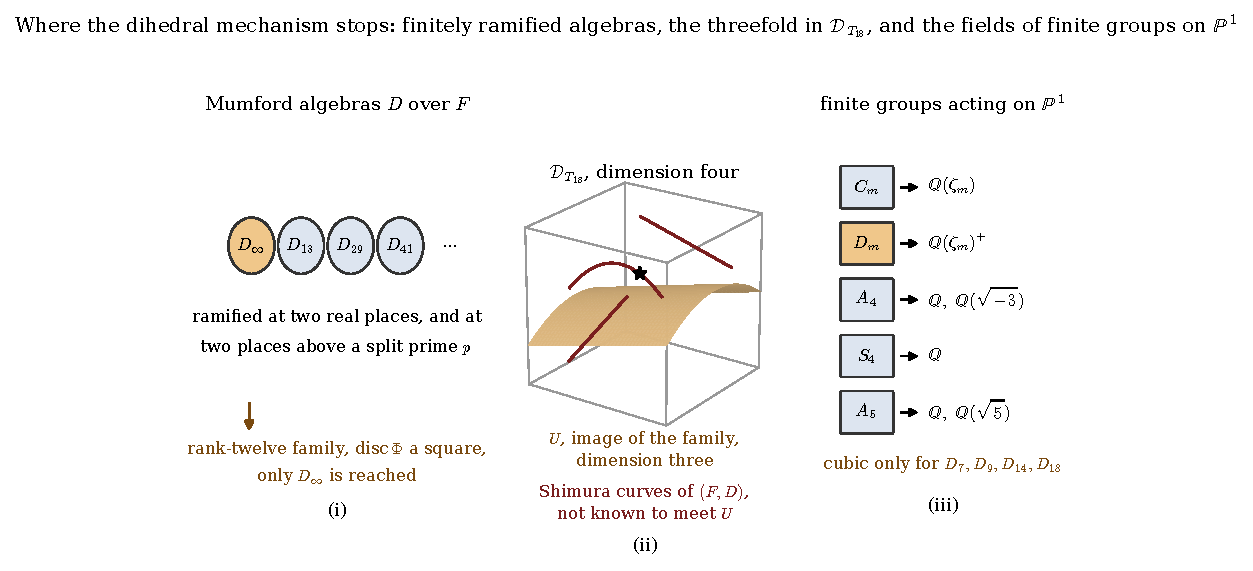
\includegraphics[width=0.92\textwidth]{figures/fig_cubicstop}
\caption{Where the dihedral mechanism stops, Proposition~\ref{prop:cubicstop}. (i)~Over $F=\QQ(\zeta_{7})^{+}$ or $\QQ(\zeta_{9})^{+}$ the Mumford algebras are $D_{\infty}$ and the algebras $D_{p}$ ramified at two real places and at two places above a split prime $p$; a rank-twelve family unimodular away from $p_{n}$ has square discriminant and carries only $D_{\infty}$. (ii)~The period domain of the rank-eighteen family is four-dimensional, the image of the family is a threefold, and the Shimura curves of the surfaces of Mumford type for the other algebras lie in the domain; whether the threefold meets them is the open transport condition. (iii)~The finite subgroups of $\mathrm{PGL}_{2}$ acting on the base produce only $\QQ(\zeta_{m})$, $\QQ(\zeta_{m})^{+}$, $\QQ$, $\QQ(\sqrt{-3})$ and $\QQ(\sqrt5)$; a cubic field arises only from the dihedral groups $D_{7}$, $D_{9}$, $D_{14}$ and $D_{18}$.}
\label{fig:cubicstop}
\end{figure*}

For the fourfolds $X$ of $(F,D_{\infty})$ the theorem leaves \Fii{} where it was: by Theorem~\ref{thm:link}(v) their exceptional classes are algebraic as soon as one algebraic cycle on $S_{\lambda}\times X^{r}$ acts nontrivially on $T(S_{\lambda})$, and the real multiplication, now algebraic, supplies no such cycle.

\subsection{Powers of K3 surfaces and Kummer type}\label{ssec:powers}

The theorems of this section decide $S\times S$ and $S^{[2]}$. On the higher powers the Hodge classes are described by Varesco \cite[Thm.~2.16]{Var25}. Let $E$ be totally real, $m=\dim_{E}T$, and for each real embedding $\sigma$ of $E$ let $V_{\sigma}=T\otimes_{E,\sigma}\CC$, so that $T_{\CC}=\bigoplus_{\sigma}V_{\sigma}$. The line $\bigwedge^{m}V_{\sigma}\subset T_{\CC}^{\otimes m}$ is spanned by a class $\det V_{\sigma}$ of type $(m,m)$, and the span of the $\det V_{\sigma}$ over all $\sigma$ is defined over $\QQ$: it is $\bigwedge^{m}_{E}T\subset\bigwedge^{m}T\subset T^{\otimes m}$, a space of Hodge classes of dimension $[E:\QQ]$ in $H^{2m}(S^{m})$, the exceptional classes. Varesco's theorem is that every Hodge class in the tensor algebra of $T$ is obtained from the Hodge classes of $T\otimes T$, which are the elements of $E$, and from the exceptional classes by tensor products, permutations of the factors, linear combinations and contractions with $q_{S}$. Each of these operations carries algebraic classes on powers of $S$ to algebraic classes: a tensor product is an exterior product, a permutation is the pull-back along an automorphism of $S^{k}$, and the contraction of two factors is the push-forward along the projection $S^{k}\to S^{k-2}$ after cupping with the pull-back of the class of the diagonal of $S\times S$, since $q_{S}(a,b)=\int_{S\times S}(a\otimes b)\cup[\Delta_{S}]$.

\begin{proposition}[Hodge classes on the powers]\label{prop:powers}
Let $S$ be a projective K3 surface with $E$ totally real and $m=\dim_{E}T$, so that $m\ge3$ as in the proof of Theorem~\ref{thm:sqrt6}(ii).
\begin{enumerate}[label=\textup{(\roman*)},leftmargin=2.4em,itemsep=2pt]
\item The Hodge conjecture holds for every power $S^{n}$ if and only if the elements of $E$ are algebraic on $S\times S$ and the exceptional classes $\bigwedge^{m}_{E}T\subset H^{2m}(S^{m})$ are algebraic. When $E=\QQ$, $m=r=\mathrm{rk}\,T$ and the exceptional class is the determinant $\det T$, which spans $\bigwedge^{r}T\subset H^{2r}(S^{r})$.
\item For a surface of Theorems~\ref{thm:sqrt6}, \ref{thm:zeta9} or Corollary~\ref{cor:dihedral} with $E$ totally real, $E$ is algebraic, and the Hodge conjecture for all powers of $S$ is equivalent to the algebraicity of $\bigwedge^{m}_{E}T$, $m=\mathrm{rk}\,T/[E:\QQ]$: $m=3$ for the surfaces $S_{\lambda}$ of Theorem~\ref{thm:zeta9}, with $\mathrm{rk}\,T=9$; $m=4$ for the very general members of the two-dimensional family of Theorem~\ref{thm:zeta9}, with $\mathrm{rk}\,T=12$.
\end{enumerate}
\end{proposition}

\begin{proof}
(i) If the Hodge conjecture holds on all powers, both kinds of classes are algebraic, being Hodge classes on $S\times S$ and on $S^{m}$. Conversely, $H^{2}(S)=\NS(S)_{\QQ}\oplus T$, and $H^{0}(S)$, $\NS(S)_{\QQ}$ and $H^{4}(S)$ are spanned by algebraic classes and are Tate twists of trivial Hodge structures. So a Hodge class of $H^{*}(S^{n})=\bigotimes^{n}\bigl(H^{0}\oplus\NS_{\QQ}\oplus T\oplus H^{4}\bigr)$ is a sum of exterior products of algebraic classes with Hodge classes of the tensor powers $T^{\otimes k}$, $k\le n$, pulled back along the projections of $S^{n}$ onto $k$ of its factors. By Varesco's theorem and the remark preceding the proposition, the Hodge classes of $T^{\otimes k}$ are algebraic as soon as $E$ and the exceptional classes are. When $E=\QQ$ there is one embedding, $V_{\sigma}=T_{\CC}$ and $\bigwedge^{m}_{E}T=\bigwedge^{r}T$.

(ii) The theorems cited prove that $E$ is algebraic; $m=\mathrm{rk}\,T/[E:\QQ]$ since $T$ is an $E$-vector space. The ranks are those of the nine-dimensional space $D_{\infty}^{0}$ and of the lattice $T_{0}$ in Step~1 of the proof of Theorem~\ref{thm:zeta9}.
\end{proof}

\begin{proposition}[K3 surfaces of Kummer type over $\QQ$]\label{prop:kummerq}
Let $S$ be a projective K3 surface, $r=\mathrm{rk}\,T$, let $\langle a_{1},\dots,a_{r}\rangle$ be a diagonalisation of $q_{S}$ on $T$, $d(T)=\prod_{i}a_{i}\in\QQ^{\times}/\QQ^{\times2}$ its discriminant and $\varepsilon_{p}(T)=\prod_{i<j}(a_{i},a_{j})_{p}$ its Hasse invariant at the prime $p$. The following are equivalent.
\begin{enumerate}[label=\textup{(\alph*)},leftmargin=2.4em,itemsep=2pt]
\item $T$ embeds isometrically in $U_{\QQ}^{3}$, the quadratic space $H^{2}(A,\QQ)$ of an abelian surface.
\item There is a dominant rational map from $S$ to a Kummer surface.
\item $r\le3$; or $r=4$ and $\varepsilon_{p}(T)=(-1,-1)_{p}$ at every prime $p$ at which $d(T)$ is a square in $\QQ_{p}$; or $r=5$ and $\varepsilon_{p}(T)=(-1,-1)_{p}$ at every prime $p$.
\end{enumerate}
Here $(-1,-1)_{p}=1$ for $p$ odd and $(-1,-1)_{2}=-1$, so (c) asks for $\varepsilon_{p}(T)=1$ at the odd primes concerned and $\varepsilon_{2}(T)=-1$. If (a)--(c) hold, then $S$ lies in the class $\mathcal{A}$ of Proposition~\ref{prop:f3prime-known}, \Fiii{} holds for every power $S^{n}$, and the Hodge conjecture holds for every $S^{n}$ and every Hilbert scheme $S^{[n]}$.
\end{proposition}

The equivalence of (a) and (b) is Ma's theorem \cite[Prop.~3.2]{Ma12}, where (a) is also shown equivalent to an embedding of lattices $T(S)\hookrightarrow U^{3}$, and for a Kummer surface itself the Hodge conjecture on all powers follows from that on the powers of the abelian surface \cite[\S0.2]{Var25}. What is added here is the form (c) of the condition, which reads it off the invariants of $T$, and the passage from Ma's rational map to the class $\mathcal{A}$.

\begin{proof}
(a)$\Leftrightarrow$(c). The space $V=U_{\QQ}^{3}\cong\langle1,-1\rangle^{3}$ has signature $(3,3)$, discriminant $-1$ and Hasse invariants $\varepsilon_{p}(V)=(-1,-1)_{p}^{3}=(-1,-1)_{p}$. By Witt's theorem $T$ embeds in $V$ if and only if there is a quadratic space $W$ over $\QQ$ with $T\oplus W\cong V$, and by the Hasse--Minkowski theorem \cite[Ch.~IV, Thm.~9]{Ser73} this is a condition on invariants: $W$ must have dimension $6-r$, signature $(1,5-r)$, discriminant $d(W)=d(V)d(T)^{-1}=-d(T)$ and, from $\varepsilon_{p}(T\oplus W)=\varepsilon_{p}(T)\varepsilon_{p}(W)(d(T),d(W))_{p}$ with $(d(T),-d(T))_{p}=1$, Hasse invariants $\varepsilon_{p}(W)=(-1,-1)_{p}\,\varepsilon_{p}(T)$. The signature forces $r-2\le3$. A quadratic space over $\QQ$ with prescribed dimension $k$, signature, discriminant and Hasse invariants exists if and only if the invariants satisfy the product formula, the real invariants are those of the signature, and at every prime the local existence condition holds \cite[Ch.~IV, \S2.3, Prop.~6, and \S3.3, Prop.~7]{Ser73}; the first two conditions hold here because they hold for $T$ and for $V$ and $T\otimes\RR\oplus W\otimes\RR\cong V\otimes\RR$, and the local condition is empty for $k\ge3$, is $\varepsilon_{p}(W)=1$ at every $p$ at which $d(W)=-1$ in $\QQ_{p}^{\times}/\QQ_{p}^{\times2}$ for $k=2$, and is $\varepsilon_{p}(W)=1$ at every $p$ for $k=1$. With $k=6-r$, $d(W)=-d(T)$ and $\varepsilon_{p}(W)=(-1,-1)_{p}\varepsilon_{p}(T)$ these are the three cases of (c).

(b) and the class $\mathcal{A}$. Let $f\colon S\dashrightarrow\mathrm{Km}(A)$ be dominant. By Lemma~\ref{lem:dominant}, $f^{*}=\Gamma_{f*}^{t}$ maps $T(\mathrm{Km}(A))_{\QQ}$ onto $T$. Let $\beta\colon\tilde A\to A$ be the blow-up of the sixteen points of order two and $\pi\colon\tilde A\to\mathrm{Km}(A)$ the quotient by the involution; $\Gamma_{A}=(\beta\times\pi)_{*}[\tilde A]$ is an algebraic cycle on $A\times\mathrm{Km}(A)$ with $\Gamma_{A*}=\pi_{*}\beta^{*}$, and $H^{2}(\mathrm{Km}(A),\QQ)=\pi_{*}\beta^{*}H^{2}(A,\QQ)\oplus\bigoplus_{i=1}^{16}\QQ[E_{i}]$ with $E_{i}$ the exceptional curves. Hence $T\subseteq(\Gamma_{f}^{t}\circ\Gamma_{A})_{*}H^{2}(A,\QQ)$, and $H^{2}(S)=\NS(S)_{\QQ}\oplus T$ is spanned by this image and by divisor classes, while $H^{0}(S)$ and $H^{4}(S)$ are spanned by the class of $S$ and the class of a point. So $S\in\mathcal{A}$, the point being the abelian variety of dimension zero, $S^{n}\in\mathcal{A}$ and \Fiii{} holds on $S^{n}$ by Proposition~\ref{prop:f3prime-known}. For the Hodge conjecture, the proof of Proposition~\ref{prop:f3prime-known}(i) writes a Hodge class of $S^{n}$ as $\sum_{j}\Gamma_{j*}y_{j}$ with $y_{j}$ a Hodge class on one of the abelian varieties spanning $H^{*}(S^{n})$, here the powers $A^{k}$ with $k\le n$. The Hodge conjecture holds for every product of surfaces with $p_{g}=1$ and $q=2$ \cite{RM08}, in particular for $A^{k}$, so every $y_{j}$, and with it every Hodge class of $S^{n}$, is algebraic. The Chow motive of $S^{[n]}$ is a direct summand of a sum of Tate twists of the motives $h(S^{k})$, $k\le n$ \cite{dCM02}, so every Hodge class of $S^{[n]}$ is the image under an algebraic correspondence of a Hodge class of some $S^{k}$.
\end{proof}

\begin{remark}[The powers left open]\label{rem:detfrontier}
(i) At $\rho(S)\ge19$ the condition (c) is empty and $S$ has a Shioda--Inose structure \cite{Mor84}. At $\rho(S)=17$ or $18$ it is a condition on the Hasse invariants, met by $U_{\QQ}^{2}\oplus\langle-2\rangle$, by $U_{\QQ}\oplus\langle2,-2,-2\rangle$ and by $\langle2,2,-2,-2\rangle$, and failed at $p=2$ and $p=3$ by $\langle2,2,-6,-6\rangle$, by $\langle2,2,-2,-6,-6\rangle$ and by $\langle2,6,-2,-2,-2\rangle$, the primes of failure coming in pairs by the product formula; all six are transcendental lattices of K3 surfaces of Picard number $18$ or $17$ by \cite{Nik80} and the surjectivity of the period map. For $r\le5$ a totally real $E$ is $\QQ$, since $m\ge3$; so $E$ is $\QQ$ or a CM field, and in the CM case the Hodge conjecture holds on all powers of $S$ with or without (c) \cite{RM08}. At $\rho\ge17$ the surfaces for which the Hodge conjecture on all powers is not decided by Propositions~\ref{prop:powers} and \ref{prop:kummerq} are therefore those with $E=\QQ$ and $T$ failing (c), and for them the one class left is $\det T\in H^{2r}(S^{r})$, $r\in\{4,5\}$. For $\rho\le16$ no surface is of Kummer type.

(ii) The Fricke surfaces have complex multiplication by $K=\QQ(\sqrt{-N})$ at every member, and Theorem~\ref{thm:fricke}(iii) settles the Hodge conjecture on all their powers. Their transcendental spaces $U_{\QQ}^{2}\oplus\langle-1\rangle\oplus\langle-N\rangle$ (Proposition~\ref{prop:frickeks}) have discriminant $N$, so they are neither of Kummer type nor in the two families of Picard number $16$ for which Varesco proves the Hodge conjecture on all powers from the algebraicity of the Kuga--Satake correspondence \cite[Thm.~4.3, Exs.~4.4, 4.5]{Var25}, whose transcendental spaces $U_{\QQ}^{2}\oplus\langle-2\rangle^{2}$ and $U_{\QQ}^{2}\oplus\langle-6\rangle\oplus\langle-2\rangle$ have discriminants $1$ and $3$ modulo squares; they are settled by the complex multiplication instead. For each surface of Proposition~\ref{prop:powers}(ii) the exceptional classes are Hodge classes of degree $2m$ on $S^{m}$ reached by no correspondence of this section, all of which act on $T\otimes T$; whether they are algebraic, and with it whether \Fiii{} and the Hodge conjecture hold on $S^{m}$, is open. The one construction known to produce such classes is the Kuga--Satake correspondence, through which Varesco proves \cite[Thm.~4.3]{Var25}.
\end{remark}

\begin{proposition}[The transcendental lattice and the Kuga--Satake variety of the Fricke surfaces]\label{prop:frickeks}
Let $N\in\{5,7\}$, $K=\QQ(\sqrt{-N})$, let $M$ be the trivial lattice $U\oplus A_{4}\oplus A_{1}^{2}\oplus D_{4}^{2}$ or $U\oplus A_{6}\oplus D_{4}^{2}$ of the elliptic fibration of the members of $\mathfrak{A}_{N}$, and let $T=M^{\perp}_{\QQ}\subset H^{2}(X,\QQ)$, which is $T(X)_{\QQ}$ when $\rho(X)=16$.
\begin{enumerate}[label=\textup{(\roman*)},leftmargin=2.4em,itemsep=2pt]
\item $T\cong U_{\QQ}^{2}\oplus\langle-1\rangle\oplus\langle-N\rangle$ as a quadratic space over $\QQ$, so $d(T)=N$ and the centre of the even Clifford algebra $C^{+}(T)$ is $K$.
\item The Kuga--Satake variety of $T$ is isogenous to $B^{4}$ for an abelian fourfold $B$ of $K$-Weil type with discriminant one. If $\rho(X)=16$ and $\End_{\Hdg}T=K$, then $B$ is isogenous to $E_{K}\times B_{3}$, where $E_{K}$ is an elliptic curve with complex multiplication by $K$ and $B_{3}$ is a simple abelian threefold with $\End(B_{3})_{\QQ}=K$; in particular $B$ is not simple.
\end{enumerate}
\end{proposition}

\begin{proof}
(i) The root lattices are rationally diagonal: $D_{n}=\{x\in\ZZ^{n}:\sum x_{i}\in2\ZZ\}$ has index two in $\ZZ^{n}$, so $D_{n}\otimes\QQ\cong\langle1\rangle^{n}$, and $E_{8}\supset D_{8}$ with index two gives $E_{8}\otimes\QQ\cong\langle1\rangle^{8}$; $A_{n}=\{x\in\ZZ^{n+1}:\sum x_{i}=0\}$ is the orthogonal complement of the vector $(1,\dots,1)$ of norm $n+1$, so $(A_{n}\oplus\langle n+1\rangle)\otimes\QQ\cong\langle1\rangle^{n+1}$; and $A_{1}^{2}=\langle2,2\rangle\cong\langle1,1\rangle$ by the vectors $(1,1)$ and $(1,-1)$ of $\ZZ^{2}$. Hence, with all forms taken positive definite, $A_{4}\oplus A_{1}^{2}\oplus D_{4}^{2}\oplus\langle1,5\rangle\cong\langle1\rangle^{5}\oplus\langle1\rangle^{2}\oplus\langle1\rangle^{8}\oplus\langle1\rangle=\langle1\rangle^{16}$ and $A_{6}\oplus D_{4}^{2}\oplus\langle1,7\rangle\cong\langle1\rangle^{7}\oplus\langle1\rangle^{8}\oplus\langle1\rangle=\langle1\rangle^{16}$ over $\QQ$. The K3 lattice is $\Lambda=U^{3}\oplus E_{8}(-1)^{2}$, so $\Lambda_{\QQ}\cong U_{\QQ}^{3}\oplus\langle-1\rangle^{16}$, while $M_{\QQ}\oplus U_{\QQ}^{2}\oplus\langle-1,-N\rangle\cong U_{\QQ}^{3}\oplus\langle-1\rangle^{16}$ by the two isometries just written. Thus $M_{\QQ}\oplus T\cong\Lambda_{\QQ}\cong M_{\QQ}\oplus(U_{\QQ}^{2}\oplus\langle-1,-N\rangle)$, and Witt's cancellation theorem gives $T\cong U_{\QQ}^{2}\oplus\langle-1\rangle\oplus\langle-N\rangle$. Its discriminant is $(-1)^{2}(-1)(-N)=N$, and the centre of $C^{+}(T)$ is $\QQ(\sqrt{(-1)^{3}d(T)})=\QQ(\sqrt{-N})$. The program \path{code/fricke_lattice.py} recomputes these isometries by the invariants of Hasse--Minkowski.

(ii) By Lombardo's theorem \cite[Thms.~6.2, 6.4]{Lom01}, in the form of \cite[Thm.~4.1]{Var25}, the Kuga--Satake variety of a polarised Hodge structure of K3 type on $U_{\QQ}^{2}\oplus\langle a\rangle\oplus\langle b\rangle$ with $a,b<0$ is isogenous to $B^{4}$ for an abelian fourfold $B$ of $\QQ(\sqrt{-ab})$-Weil type with discriminant one; here $(a,b)=(-1,-N)$, $\QQ(\sqrt{-ab})=K$ and $C^{+}(T)\cong M_{4}(K)$. Suppose $\rho(X)=16$ and $\End_{\Hdg}T=K$. By Zarhin's theorem \cite[Thm.~2.3.1]{Zar83} the Hodge group of $T$ is $G=\mathrm{U}(W,h)$, the unitary group of the hermitian form $h$ on the three-dimensional $K$-space $W=T$ with $\Tr_{K/\QQ}h=q$. Over $\CC$ the two eigenspaces $W_{\sigma}$, $W_{\bar\sigma}$ of $K$ on $T_{\CC}$ have dimension three and are isotropic for $q$, since $q(ax,y)=q(x,\bar ay)$, so $T_{\CC}=W_{\sigma}\oplus W_{\sigma}^{*}$ and $G_{\CC}=\mathrm{GL}(W_{\sigma})$ acting on $W_{\sigma}^{*}$ by the dual representation. The Kuga--Satake Hodge structure on $H^{1}(B,\QQ)$ is the lift of that of $T$ along $\mathrm{Spin}(T)\to\mathrm{SO}(T)$ \cite[\S5]{vG08}, so the Hodge group of $B$ is the preimage $\widetilde G$ of $G$ in $\mathrm{Spin}(T)$, and $H^{1}(B,\CC)=S^{+}\oplus S^{-}$ is the sum of the two half-spin representations of $\mathrm{Spin}(T_{\CC})\cong\SL_{4}$, on which the two eigenspaces of the centre $K$ of $C^{+}(T)$ are $S^{+}$ and $S^{-}$. For the isotropic decomposition $T_{\CC}=W_{\sigma}\oplus W_{\sigma}^{*}$ the spin representation is $\bigwedge^{\bullet}W_{\sigma}\otimes(\det W_{\sigma})^{-1/2}$, with $S^{+}$ the even and $S^{-}$ the odd part. Restricted to $\widetilde G_{\CC}$, $S^{+}=(\bigwedge^{0}W_{\sigma}\oplus\bigwedge^{2}W_{\sigma})\otimes\det^{-1/2}$ is the sum of the character $\chi=\det^{-1/2}$ and of the irreducible representation $W_{\sigma}^{*}\otimes\det^{1/2}$ of dimension three, and $S^{-}=(W_{\sigma}\oplus\bigwedge^{3}W_{\sigma})\otimes\det^{-1/2}$ is the sum of $W_{\sigma}\otimes\det^{-1/2}$ and of $\chi^{-1}$. The four summands are pairwise non-isomorphic, the two characters being distinct and the two three-dimensional representations having different weights, so they are the isotypic components of $H^{1}(B,\CC)$ under the connected group $\widetilde G_{\CC}$. An automorphism of $\CC$ over $\QQ$ carries an isotypic component to one of the same dimension, since the representation is defined over $\QQ$; so $U_{\CC}=\chi\oplus\chi^{-1}$ and $V_{\CC}=S^{+}\oplus S^{-}$ minus it are stable under all of them and are the complexifications of $\QQ$-subspaces $U$, $V$ with $H^{1}(B,\QQ)=U\oplus V$. Both are stable under $\widetilde G$, hence sub-Hodge structures, and under $K$, which acts by scalars on $S^{+}$ and on $S^{-}$. By Poincar\'e reducibility $B$ is isogenous to $E_{K}\times B_{3}$ with $H^{1}(E_{K},\QQ)=U$ and $H^{1}(B_{3},\QQ)=V$. The algebra $\End_{\Hdg}(U)\otimes\CC=\End(\chi)\oplus\End(\chi^{-1})$ has dimension two and contains $K$, so $\End(E_{K})_{\QQ}=K$; likewise $\End_{\Hdg}(V)\otimes\CC$ has dimension two, so $\End(B_{3})_{\QQ}=K$, a field, and $B_{3}$ is simple; and $\Hom(E_{K},B_{3})=0$ since $U$ and $V$ share no isotypic component.
\end{proof}

\begin{remark}[Real multiplication at the fixed points]\label{rem:frickefixed}
Theorem~\ref{thm:fricke}(iii) decides every power of every Fricke surface, so the Kuga--Satake variety of Proposition~\ref{prop:frickeks}(ii) is not needed for them; the proposition records what the splitting of $T$ into the two eigenspaces of $K$ does to the Kuga--Satake construction. For a very general Hodge structure of K3 type on $U_{\QQ}^{2}\oplus\langle-1\rangle\oplus\langle-N\rangle$, with endomorphism field $\QQ$, the fourfold $B$ is simple with a definite quaternion algebra as endomorphism algebra \cite[Prop.~5.7]{vG08}; the Fricke families lie in the locus of the four-dimensional period domain where the endomorphism field is $K$, and there $B$ splits. Real multiplication by $\sqrt N$ appears on the two twists at the fixed points of $w$, the surfaces of \cite[\S7.6, Prop.~7.7]{vGS25}, where $\Lambda^{2}=N$ by Lemma~\ref{lem:frickesign}(ii). A family of K3 surfaces of transcendental rank six with real multiplication by $\sqrt5$ or $\sqrt7$ on which the multiplication is algebraic is not known to us: the fixed points of $w$ are two, so the fixed-point twists are two surfaces, and Remark~\ref{rem:sqrt10} says why the chains of Theorem~\ref{thm:chain} do not supply one.
\end{remark}

\subsection{Where this stops}\label{ssec:f3stop}

The frontier case of \Fiii{} in \cite[Thm.~21.4 and Rem.~21.5]{BMB26} is a K3 surface $S_{\lambda}$ of Picard number $13$ with $T(S_{\lambda})_{\QQ}\cong T$, the nine-dimensional representation of a Mumford fourfold, and $E=F$ a totally real cubic field, which may have Galois group $S_{3}$. Theorem~\ref{thm:zeta9} settles it for the two cyclic fields $F=\QQ(\zeta_{7})^{+}$ and $\QQ(\zeta_{9})^{+}$ with the algebra $D_{\infty}$; the frontier is now $S_{\lambda}$ for every other pair $(F,D)$: for these two fields with the algebras ramified at two finite places, for the cyclic cubic fields of conductor at least $13$, and for every field that is not cyclic. There, by Proposition~\ref{prop:structure}(v), no composite of similarities reaches $F$,\footnote{Reaching $F$ means producing, by algebraic correspondences from $S_{\lambda}$ to itself, Hodge endomorphisms of $T(S_{\lambda})_{\QQ}$ that generate the cubic field $E=F$, which is what \Fiii{} asks of this surface, since the class of a generator of $F$ in $H^{4}(S_{\lambda}\times S_{\lambda})$ is a Hodge class reached from no abelian variety as long as it is not algebraic. The correspondences built in this section, and every correspondence whose components have geometric genus at most one, act on $T(S_{\lambda})$ as similarities, and a composite of similarities is a similarity; by Proposition~\ref{prop:structure}(ii) a similarity lies in $\QQ$ when $[E:\QQ]$ is odd, so it generates nothing. The correspondences coming from finite group actions act through abelian fields by Proposition~\ref{prop:hecke}(iii), and a cubic field whose Galois closure has group $S_{3}$ is not abelian. The two propositions together say what a correspondence realising $F$ must look like: an irreducible component with $p_{g}\ge2$ and transcendental rank at least eighteen, not arising from a finite group; no construction in the literature produces one.} so Theorem~\ref{thm:chain}, the Fricke isogenies and every correspondence of the kinds listed are blind to it; by Proposition~\ref{prop:structure}(iv) a correspondence that does reach it has an irreducible component whose resolution has $p_{g}\ge2$, transcendental rank at least $18$ and $b_{2}\ge31$; and by Proposition~\ref{prop:hecke}(iii) that component is not the graph of an element of a finite group acting on a cover of $S_{\lambda}$ when $F$ is not cyclic. When $F$ is cyclic the dihedral families are the natural source, as van Geemen observed for $\QQ(\zeta_{9})^{+}$ \cite[Rem.~7.9]{vG08}; Theorem~\ref{thm:zeta9} is the statement that for the two fields of conductor $7$ and $9$ and the algebra $D_{\infty}$ the source actually reaches $S_{\lambda}$, and Proposition~\ref{prop:cubicstop} says that it reaches nothing else. The only correspondences of this size that we know to act on a transcendental space of K3 type are the dihedral ones, which give abelian fields, and the Kuga--Satake correspondence into the cohomology of an abelian variety of dimension $2^{7}$, whose algebraicity is open \cite{Del72,vG00}; in Section~\ref{sec:f2} we replace its abelian variety by a sixfold and show what the replacement does and does not give. Within quadratic fields the method reaches $\sqrt d$ for $d\in\{2,3,6\}$ in families, and the Fricke isogenies give complex multiplication by $\QQ(\sqrt{-5})$ and $\QQ(\sqrt{-7})$ on one-dimensional families, where Theorem~\ref{thm:fricke} settles the Hodge conjecture on every power; real multiplication by $\sqrt5$ and $\sqrt7$ is algebraic on the two surfaces of \cite{vGS25} and on no family known to us (Remark~\ref{rem:frickefixed}); for $\QQ(\sqrt{10})$, $\QQ(\sqrt{14})$ and the other composite discriminants no family is known on which the chain of Theorem~\ref{thm:chain} can be started. On the powers beyond the square, Proposition~\ref{prop:powers} reduces the Hodge conjecture for every surface of this section with totally real endomorphism field to its exceptional classes, Proposition~\ref{prop:kummerq} settles it with \Fiii{} for the surfaces of Kummer type over $\QQ$, Theorem~\ref{thm:fricke} settles it for every member of the Fricke families, and Remark~\ref{rem:detfrontier} records what is left.

\begin{proposition}[Chains of symplectic quotients reach exactly $\sqrt2$, $\sqrt3$, $\sqrt6$]\label{prop:sqrt10}
Let $S$ be a projective K3 surface whose endomorphism field $E$ is totally real and different from $\QQ$, and let $S=S_{0},\dots,S_{r}$ be a chain as in Theorem~\ref{thm:chain} in which every rational map is the quotient by a finite group of symplectic automorphisms. Then no degree $n_{i}$ is divisible by $5$ or by $7$, every $n_{i}$ divides a power of $24$, and the multiplier $\prod n_{i}^{\pm1}$ lies in $\{1,2,3,6\}$ modulo squares. In particular no such chain makes $\sqrt{10}$, $\sqrt{14}$, $\sqrt{15}$ or $\sqrt{21}$ algebraic, and the surfaces with real multiplication by these fields are not reached by Theorem~\ref{thm:chain} in this form.
\end{proposition}

\begin{proof}
Along the chain the transcendental spaces are isomorphic up to scaling of the form, by Lemma~\ref{lem:dominant} and Lemma~\ref{lem:isometry}, so every $S_{i}$ has the same transcendental rank $t$ and the same endomorphism field $E$ as $S$. By Zarhin \cite[Thms.~2.2.1 and 2.3.1]{Zar83} the Hodge group of $T(S)_{\QQ}$ is the group of $E$-linear special isometries of the $E$-quadratic space $W$ with $T(S)_{\QQ}=\mathrm{Tr}_{E/\QQ}W$, of dimension $m=t/[E:\QQ]$ over $E$. If $m\le2$ this group is commutative (trivial for $m=1$, a torus of dimension $[E:\QQ]$ for $m=2$). Then every $g\in\mathrm{Hdg}(\QQ)$ commutes with the Hodge group and is an endomorphism of the Hodge structure, so $g\in E$. The elements of the totally real field $E$ are self-adjoint for the form on $T(S)_{\QQ}$ and $g$ is an isometry, so $g=g^{*}=g^{-1}$ and $g^{2}=1$. As $\QQ$-points are Zariski dense in a connected linear algebraic group over $\QQ$, the Hodge group would be trivial, which is impossible because $h^{2,0}(S)=1$. So $m\ge3$ and $t\ge3[E:\QQ]\ge6$.

Let $G$ be a finite group of symplectic automorphisms of a K3 surface $X$ and $\Omega_{G}\subset\NS(X)$ its coinvariant lattice, negative definite because $G$ fixes the transcendental lattice and an ample class. If $5$ divides $|G|$, then $G$ contains an element of order five, whose coinvariant lattice has rank $16$ \cite[\S\,5]{Nik80b} and lies in $\Omega_{G}$, so $\mathrm{rk}\,\Omega_{G}\ge16$; if $7$ divides $|G|$ the same argument with the rank $18$ of an element of order seven gives $\mathrm{rk}\,\Omega_{G}\ge18$. The transcendental lattice $T(X)$ lies in $\Omega_{G}^{\perp}\subset H^{2}(X,\ZZ)$, which has rank $22-\mathrm{rk}\,\Omega_{G}\le6$ and signature $(3,19-\mathrm{rk}\,\Omega_{G})$, and $T(X)$ has signature $(2,\mathrm{rk}\,T(X)-2)$; so $\mathrm{rk}\,T(X)\le5$ when $5$ divides $|G|$ and $\mathrm{rk}\,T(X)\le3$ when $7$ does. Every symplectic automorphism of finite order has order at most eight \cite{Nik80b}, so if some $n_{i}=|G_{i}|$ is not of the form $2^{a}3^{b}$ then $5$ or $7$ divides it, the source of that quotient has transcendental rank at most five, and so has $S$; this contradicts $t\ge6$. Hence every $n_{i}$ is of the form $2^{a}3^{b}$, and the multiplier is $2^{a}3^{b}$ modulo squares, that is $1$, $2$, $3$ or $6$. A multiplier $n$ makes only $e$ with $e^{2}\equiv n$ algebraic, which gives the list.
\end{proof}

\begin{remark}\label{rem:sqrt10}
The proposition settles the lattice question of whether a chain $S\to Y\leftarrow S'$ through a symplectic involution and a symplectic automorphism of order five, of multiplier $2/5\equiv10$, can start on a surface with real multiplication by $\QQ(\sqrt{10})$: it cannot, since $S'$ would have transcendental rank at most five and real multiplication by a real quadratic field needs rank at least six. The same bound shows that the surfaces of transcendental rank at most five with a symplectic automorphism of order five or seven have endomorphism field $\QQ$ or a CM field; in the CM case the Hodge group is a torus and the chain closes only through the complex multiplication itself. Real multiplication by $\sqrt{10}$, $\sqrt{14}$ or any field outside $\{\QQ(\sqrt2),\QQ(\sqrt3),\QQ(\sqrt5),\QQ(\sqrt6),\QQ(\sqrt7)\}$, and by $\sqrt5$ or $\sqrt7$ beyond the two surfaces of \cite{vGS25}, therefore needs a correspondence that is not a composite of symplectic quotients, Hodge isometries and fibrewise isogenies, and none is known to us.
\end{remark}

\section{Constructions at \Fii{}}\label{sec:f2}

The first classes \Fii{} has to reach are the Weil classes of a very general abelian $2n$-fold of Weil type with $n\ge3$, and the exceptional classes of a Mumford fourfold. We build an object at each.

\subsection{The polarised semiregularity criterion}\label{ssec:criterion}

Let $A$ be a very general member of the polarised family $\cD_{n,n}$ of abelian $2n$-folds of Weil type for an imaginary quadratic field $K$, with polarisation class $\theta$ and Weil plane $W(A)$. Then $\Hdg^{*}(A)=\QQ[\theta]\oplus W(A)$ and $W(A)\cdot\theta=0$ \cite[Thm.~4.14]{BMB26}. A class $\gamma\in H^{\mathrm{ev}}(A)$ has the polarised shape if
\[
\gamma=N\omega+\sum_{k=0}^{2n}c_{k}\theta^{k},\qquad N\ne0,\ 0\ne\omega\in W(A),\ c_{k}\in\QQ .
\]
Its Hankel rank $\rho\in\{0,1,2,3\}$ is the rank of the Hankel matrix of the sequence $(k!\,c_{k})_{k}$ capped at three; it is the number of distinct exponentials $e^{a\theta}$ needed to write the polynomial part when that number is at most two, and $3$ otherwise.\footnote{The Hankel matrix of a sequence $(a_{k})_{k\ge0}$ has entries $a_{i+j}$. If $a_{k}$ is a sum $\sum_{j}\lambda_{j}b_{j}^{k}$ of $m$ terms with distinct $b_{j}$ and nonzero $\lambda_{j}$, the matrix factors as $V^{\mathsf{T}}\operatorname{diag}(\lambda_{j})V$ with $V$ the Vandermonde matrix of the $b_{j}$, so its rank is $m$; conversely a sequence whose Hankel matrix has finite rank $m$ satisfies a linear recurrence of order $m$ and is a sum of $m$ exponentials with polynomial coefficients. For the polynomial part $\sum_{k}c_{k}\theta^{k}$ of a Chern character, writing it as $\sum_{j}\lambda_{j}e^{b_{j}\theta}$ means $k!\,c_{k}=\sum_{j}\lambda_{j}b_{j}^{k}$, so the number of exponentials needed is the Hankel rank of $(k!\,c_{k})$, provided the degree $2n$ allows the recurrence to be read off, which it does for $m\le2$; the cap at three records that the criterion of Theorem~\ref{thm:criterion} does not distinguish further.}

\begin{theorem}[The polarised criterion \protect{\cite{BMB26}}]\label{thm:criterion}
Let $\mathcal{E}$ be a perfect complex on $A$ with $\ch(\mathcal{E})=\gamma$ of polarised shape and Hankel rank $\rho$. Then
\[
\dim\Ext^{2}(\mathcal{E},\mathcal{E})\ \ge\ r(\gamma):=(4+\rho)\,n^{2}-2n,
\]
and if equality holds the semiregularity map\footnote{For a perfect complex $\mathcal{E}$ on a smooth projective variety the semiregularity map of Buchweitz and Flenner \cite{BF03} is the linear map $\sigma_{\mathcal{E}}\colon\Ext^{2}(\mathcal{E},\mathcal{E})\to\prod_{q}H^{q+1}(X,\Omega^{q-1}_{X})$ sending $\xi$ to the trace of $\xi\circ\exp\bigl(-\mathrm{At}(\mathcal{E})\bigr)$, where $\mathrm{At}(\mathcal{E})\in\Ext^{1}(\mathcal{E},\mathcal{E}\otimes\Omega^{1}_{X})$ is the Atiyah class; it generalises Bloch's map for a subvariety \cite{Blo72}, which is the case of the structure sheaf of the subvariety. Its value is that the obstruction to deforming $\mathcal{E}$ along a first-order deformation of $X$ lies in $\Ext^{2}(\mathcal{E},\mathcal{E})$ and is sent by $\sigma_{\mathcal{E}}$ to the obstruction to keeping $\ch(\mathcal{E})$ of Hodge type; so when $\sigma_{\mathcal{E}}$ is injective, $\mathcal{E}$ deforms wherever its Chern character stays a Hodge class, and the Chern character of the deformed complex is algebraic there. The dimension count of the theorem is the arithmetic of this statement: the rank of $\sigma_{\mathcal{E}}$ is at least the rank of the contraction into $\ch(\mathcal{E})$, so $\dim\Ext^{2}$ is at least $r(\gamma)$, and equality forces injectivity.} of $\mathcal{E}$ is injective, $\mathcal{E}$ deforms with $A$ along the whole of $\cD_{n,n}$, and the Weil classes are algebraic on every member of the family with full Hodge group. If some $c_{k}\ne0$ with $1\le k\le 2n-1$, the first-order Hodge locus of $\gamma$ in $H^{1}(A,T_{A})$ is the tangent space of $\cD_{n,n}$, of dimension $n^{2}$. A perfect complex whose Chern character is exactly a multiple of a Weil class does not exist on a very general member, so the polynomial part is forced.
\end{theorem}

The number $r(\gamma)$ is the rank of the contraction $HT^{2}(A)\to H^{*}(A)$, $\xi\mapsto\xi\lrcorner\gamma$, on the Hochschild cohomology $HT^{2}=\bigoplus_{p+q=2}H^{q}(A,\bigwedge^{p}T_{A})$, of dimension $\binom{4n}{2}$; its kernel is the annihilator $\mathrm{Ann}(\gamma)$, which meets $H^{1}(A,T_{A})$ in the first-order Hodge locus. The semiregularity map $\sigma_{\mathcal{E}}$ of a perfect complex composes with the characteristic map $\mathrm{ev}_{\mathcal{E}}:HT^{2}\to\Ext^{2}(\mathcal{E},\mathcal{E})$, $\xi\mapsto\xi\lrcorner\mathrm{At}(\mathcal{E})$, to the contraction into $\ch(\mathcal{E})$; this is how the lower bound arises, and it is the form in which the criterion is used below. Figure~\ref{fig:hankel} shows $r(\gamma)$; the two values that matter below are $r=57$ at $n=3$, $\rho=3$ and $r=104$ at $n=4$, $\rho=3$. On the product $E_{0}^{6}$ of six copies of the elliptic curve $\CC/\ZZ[i]$ every twisted complex of line bundles has $\dim\Ext^{2}\ge69>57$ \cite[Thm.~18.35]{BMB26}; the criterion is not met there by any such object.

\begin{figure*}[t]
\centering
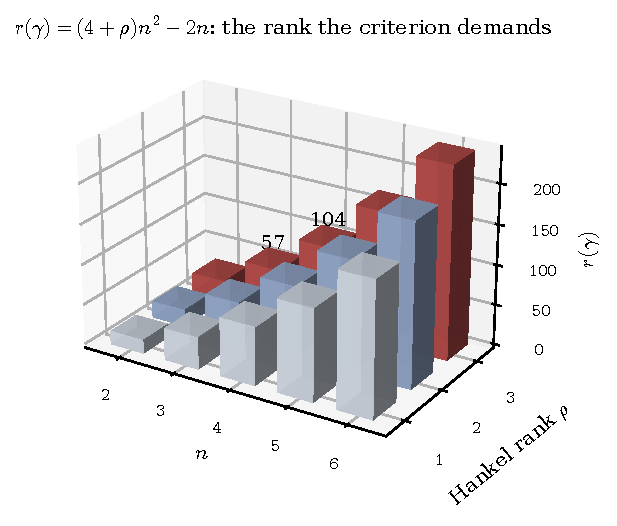
\includegraphics[width=0.78\textwidth]{figures/fig_hankel}
\caption{The lower bound $r(\gamma)=(4+\rho)n^{2}-2n$ of Theorem~\ref{thm:criterion} for $2\le n\le6$ and Hankel rank $\rho=1,2,3$. The two labelled bars are the product cases of Theorem~\ref{thm:product}.}
\label{fig:hankel}
\end{figure*}

\subsection{The Weil plane of a product}

\begin{lemma}\label{lem:weilproduct}
Let $A$, $A'$ be of Weil type for the same field $K$, of dimensions $2m$, $2m'$, with the diagonal $K$-action on $A\times A'$. Then $W(A\times A')$ is a two-dimensional rational subspace of the four-dimensional space $W(A)\otimes W(A')\subseteq H^{2n}(A\times A')$, $n=m+m'$, and every rational $w\in W(A\times A')$ is $\sum_{i,j}a_{ij}\,\omega_{i}\otimes\omega'_{j}$ with $a_{ij}\in\QQ$ for rational bases $(\omega_{i})$, $(\omega'_{j})$ of $W(A)$, $W(A')$.
\end{lemma}

\begin{proof}
Over $\CC$, $H^{1}(A\times A')=V\oplus V'$ splits into eigenspaces $V_{\pm}\oplus V'_{\pm}$ of $K$, and $\bigwedge^{2n}_{K}$ of the sum is spanned by $\det V_{+}\otimes\det V'_{+}$ and $\det V_{-}\otimes\det V'_{-}$; these lie in the span of the four products $\omega_{\pm}\otimes\omega'_{\pm}$ of the eigenvectors of $W(A)\otimes\CC$ and $W(A')\otimes\CC$. Both $W(A\times A')$ and $W(A)\otimes W(A')$ are defined over $\QQ$, so the inclusion holds over $\QQ$. The explicit formula is \cite[Eq.~(36)]{BMB26}: $\omega_{1}(A\times A')=\omega_{1}\otimes\omega'_{1}-d\,\omega_{2}\otimes\omega'_{2}$ for $K=\QQ(\sqrt{-d})$.
\end{proof}

\subsection{An object with the polarised Chern character}

\begin{theorem}[The product object]\label{thm:product}
Let $A$, $A'$ be very general in their polarised Weil families, with ample classes $\theta_{A}$, $\theta_{A'}$, $\theta=\theta_{A}+\theta_{A'}$, and suppose that $W(A)$ and $W(A')$ are algebraic. Then there is a perfect complex $\mathcal{E}$ on $A\times A'$, a finite direct sum with shifts of exterior products
\[
F_{i}\boxtimes G'_{j},\quad F_{i}\boxtimes L'^{\,k},\quad L^{l}\boxtimes G'_{j},\quad L^{l}\boxtimes L'^{\,k},
\]
with $F_{i}$, $G'_{j}$ coherent sheaves on $A$, $A'$ and $L$, $L'$ the ample bundles, such that
\[
\ch(\mathcal{E})=N\,w+\sum_{k=0}^{2n}c_{k}\theta^{k},\qquad N\ne0,\ 0\ne w\in W(A\times A'),
\]
has the polarised shape with Hankel rank $\rho=3$, so that $r(\ch\mathcal{E})=7n^{2}-2n$, and the first-order Hodge locus of $\ch(\mathcal{E})$ in $H^{1}(A\times A',T)$ is the tangent space of $\cD_{n,n}$.
\end{theorem}

The hypotheses hold in the two open cases nearest to the known ones: $A$, $A'$ very general Weil fourfolds of trivial discriminant, where the Weil classes are algebraic by Markman's theorem for discriminant one \cite{Mar23} and the specialisation of algebraic classes, so that $A\times A'$ is an eightfold with $n=4$; and $A$ such a fourfold and $A'=B$ a Weil surface of any discriminant $d$, whose Weil plane is of type $(1,1)$ and algebraic by Lefschetz, so that $A\times B$ is a sixfold of discriminant $d$ with $n=3$.

\begin{proof}
Since $\Hdg^{*}(A)=\QQ[\theta_{A}]\oplus W(A)$, algebraic classes on $A$ are rational combinations of Chern characters of coherent sheaves, and the Chern character of a coherent sheaf is a Hodge class, the algebraicity of $W(A)$ gives coherent sheaves $F_{1}$, $F_{2}$ with $\ch(F_{i})=N_{i}\omega_{i}+p_{i}(\theta_{A})$, $N_{i}\ne0$, for a basis $(\omega_{1},\omega_{2})$ of $W(A)$; likewise $G'_{1}$, $G'_{2}$ on $A'$ with $\ch(G'_{j})=N'_{j}\omega'_{j}+p'_{j}(\theta_{A'})$. Fix $0\ne w\in W(A\times A')$ rational, $w=\sum a_{ij}\omega_{i}\otimes\omega'_{j}$ by Lemma~\ref{lem:weilproduct}, and a common denominator $M$ of the numbers $Ma_{ij}/(N_{i}N'_{j})$, so that these are integers. Negative multiplicities are realised by the shift $[1]$, which changes the sign of $\ch$.

Step 1. $\mathcal{E}_{0}=\bigoplus_{i,j}(F_{i}\boxtimes G'_{j})^{\oplus Ma_{ij}/(N_{i}N'_{j})}$ has, by multiplicativity,
\begin{widetext}
\begin{equation}\label{eq:chE0}
\ch(\mathcal{E}_{0})=Mw+\sum_{i}\omega_{i}\otimes q'_{i}(\theta_{A'})+\sum_{j}q_{j}(\theta_{A})\otimes\omega'_{j}+s,
\end{equation}
\end{widetext}
with $q'_{i}$, $q_{j}$ polynomials and $s\in\QQ[\theta_{A}]\otimes\QQ[\theta_{A'}]$.

Step 2. The classes $e^{k\theta_{A'}}=\ch(L'^{\,k})$, $k=0,\dots,2m'$, form a basis of $\QQ[\theta_{A'}]/(\theta_{A'}^{2m'+1})$: the matrix $(k^{j}/j!)_{j,k}$ has determinant $\prod_{j}(1/j!)$ times the Vandermonde determinant of $0,1,\dots,2m'$, which is nonzero. Write $q'_{i}=\sum_{k}b_{ik}e^{k\theta_{A'}}$ and add $(F_{i}\boxtimes L'^{\,k})^{\oplus-Mb_{ik}/N_{i}}$, after enlarging $M$ to clear denominators; this removes $\omega_{i}\otimes q'_{i}$ and adds only terms $p_{i}(\theta_{A})\otimes e^{k\theta_{A'}}$, which lie in $\QQ[\theta_{A}]\otimes\QQ[\theta_{A'}]$. Symmetrically remove $q_{j}\otimes\omega'_{j}$ with summands $L^{l}\boxtimes G'_{j}$.

\begin{figure*}[t]
\centering
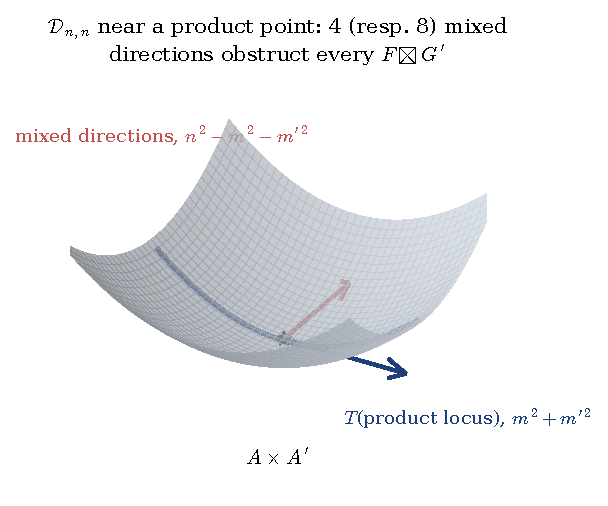
\includegraphics[width=0.78\textwidth]{figures/fig_product}
\caption{The domain $\cD_{n,n}$ near a product point $A\times A'$. The curve is the product locus, whose tangent space has dimension $m^{2}+m'^{2}$; the $2mm'$ mixed directions obstruct every exterior product $F\boxtimes G'$, and only the combined object of Theorem~\ref{thm:product} has the full tangent space as first-order Hodge locus.}
\label{fig:product}
\end{figure*}

Step 3. The classes $e^{l\theta_{A}+k\theta_{A'}}=\ch(L^{l}\boxtimes L'^{\,k})$ form a basis of $\QQ[\theta_{A}]/(\theta_{A}^{2m+1})\otimes\QQ[\theta_{A'}]/(\theta_{A'}^{2m'+1})$ by the same determinant, so the remaining part in $\QQ[\theta_{A}]\otimes\QQ[\theta_{A'}]$ is cancelled by line bundles with integer multiplicities and shifts. Finally add $(L\boxtimes L')^{\otimes k}$, $k=0,1,2$, with generic nonzero multiplicities $\mu_{k}$. The result is
\[
\ch(\mathcal{E})=Mw+\sum_{k=0}^{2}\mu_{k}e^{k\theta},
\]
a polarised shape whose polynomial part is a sum of three distinct exponentials with nonzero coefficients. Three exponentials are not one of the shapes of Hankel rank at most two, so $\rho=3$; and some $c_{k}$ with $1\le k\le2n-1$ is nonzero, so the first-order Hodge locus is the tangent space of $\cD_{n,n}$ by Theorem~\ref{thm:criterion}.
\end{proof}

The construction was carried out in the exterior-algebra model of $H^{*}(A\times A')$ for $(m,m')=(2,1)$ and $(2,2)$: the cross terms of $\ch(\mathcal{E}_{0})$ vanish, nothing is left outside $W(A\times A')\oplus\QQ[\theta]$ after Steps 2 and 3, the Hankel rank is $3$, and the first-order Hodge locus has dimension $9$, resp.\ $16$, equal to $n^{2}$ (Appendix~\ref{app:checks}).

\subsection{What a direct sum cannot do}

The tangent space of $\cD_{n,n}$ at a product point contains the tangent space of the product locus $\cD_{m,m}\times\cD_{m',m'}$, of dimension $m^{2}+m'^{2}$, and $n^{2}-m^{2}-m'^{2}=2mm'$ mixed directions. In the same model, each exterior product $F\boxtimes G'$ of sheaves of polarised shape has first-order Hodge locus inside $T\cD_{n,n}$ equal to the tangent space of the product locus: all $2mm'$ mixed directions obstruct it, four for $A\times B$ and eight for $A\times A'$ (Fig.~\ref{fig:product}). The object $\mathcal{E}$ of Theorem~\ref{thm:product} has the whole tangent space as its first-order locus because its Chern character is a single polarised class and not a product. Semiregularity is a different matter.

\begin{proposition}[Direct sums are never semiregular]\label{prop:directsum}
\leavevmode
\begin{enumerate}[label=\textup{(\roman*)},leftmargin=2.4em,itemsep=2pt]
\item Let $\mathcal{E}=\bigoplus_{k}\mathcal{E}_{k}$ be a direct sum of at least two nonzero complexes. Then the semiregularity map $\sigma_{\mathcal{E}}$ vanishes on $\bigoplus_{k\ne l}\Ext^{2}(\mathcal{E}_{k},\mathcal{E}_{l})$. So $\sigma_{\mathcal{E}}$ is injective only if $\Ext^{2}(\mathcal{E}_{k},\mathcal{E}_{l})=0$ for all $k\ne l$.
\item For every direct-sum realisation $\mathcal{E}$ of Theorem~\ref{thm:product}, $\sigma_{\mathcal{E}}$ is not injective and $\dim\Ext^{2}(\mathcal{E},\mathcal{E})>r(\ch\mathcal{E})$.
\end{enumerate}
\end{proposition}

\begin{proof}
(i) The semiregularity map of Buchweitz and Flenner is built from the traces $\xi\mapsto\mathrm{tr}\bigl(\xi\circ\mathrm{At}(\mathcal{E})^{p}\bigr)$ of compositions with powers of the Atiyah class \cite[Sect.~4]{BF03}. The Atiyah class of a direct sum is block diagonal, so for $\xi$ in an off-diagonal block $\Ext^{2}(\mathcal{E}_{k},\mathcal{E}_{l})$ the composition $\xi\circ\mathrm{At}(\mathcal{E})^{p}$ is off-diagonal, and the trace of an off-diagonal block is zero.

(ii) The summands of $\mathcal{E}$ include $F_{1}\boxtimes L'^{\,k}$ and $F_{1}\boxtimes L'^{\,l}$ for two exponents $k<l$, because Step 2 of the proof uses every power $L'^{\,k}$ with $0\le k\le2m'$ (the exponentials form a basis and $q'_{1}$ is a nonzero polynomial of positive degree for a sheaf of polarised shape, which has $p_{1}$ of positive degree by Theorem~\ref{thm:criterion}). By the K\"unneth formula
\begin{widetext}
\begin{equation}\label{eq:kunneth}
\Ext^{2}(F_{1}\boxtimes L'^{\,k},F_{1}\boxtimes L'^{\,l})\supseteq\Ext^{2}(F_{1},F_{1})\otimes H^{0}(A',L'^{\,l-k}),
\end{equation}
\end{widetext}
and $\dim\Ext^{2}(F_{1},F_{1})\ge r(\ch F_{1})\ge12$ by Theorem~\ref{thm:criterion} on the fourfold $A$ ($n=2$, $\rho\ge0$), while $H^{0}$ of an ample bundle is nonzero. So an off-diagonal block is nonzero, $\sigma_{\mathcal{E}}$ has a kernel by (i), and $\dim\Ext^{2}(\mathcal{E},\mathcal{E})>r$ because equality would force injectivity.
\end{proof}

\begin{proposition}[Convolutions]\label{prop:convolution}
Let $\mathcal{E}_{\delta}$ be a one-sided twisted complex on pieces $P_{1},\dots,P_{N}$ with shifts $s_{a}$, ordered so that the differential $\delta=(\delta_{ab})_{a<b}$, $\delta_{ab}\in\Ext^{1+s_{a}-s_{b}}(P_{a},P_{b})$, is strictly upper triangular; let $\gamma=\ch(\mathcal{E}_{\delta})=\sum_{a}(-1)^{s_{a}}\ch(P_{a})$.
\begin{enumerate}[label=\textup{(\roman*)},leftmargin=2.4em,itemsep=2pt]
\item The semiregularity map $\sigma_{\mathcal{E}_{\delta}}$ vanishes on every class of $\Ext^{2}(\mathcal{E}_{\delta},\mathcal{E}_{\delta})$ represented by a strictly upper triangular cocycle. So the criterion holds for $\mathcal{E}_{\delta}$ only if every strictly upper triangular cocycle of degree two is a coboundary.
\item Suppose no term of the twisted differential carries a class of degree one into a diagonal block $\Ext^{*}(P_{c},P_{c})$. Let $v\in T\cD_{n,n}$ have a nonzero mixed component. If some piece $P=X\boxtimes Y$ has $\operatorname{rk}Y\,c_{1}(X)/\theta_{A}\ne\operatorname{rk}X\,c_{1}(Y)/\theta_{A'}$, then $\mathrm{ev}_{\mathcal{E}_{\delta}}(v)\ne0$ and $\sigma_{\mathcal{E}_{\delta}}(\mathrm{ev}_{\mathcal{E}_{\delta}}(v))=0$: the criterion fails.
\item Suppose the pieces split into two nonempty groups with $\Ext^{*}(P_{a},P_{b})=0$ in both directions for $a$, $b$ in different groups. Then $\mathcal{E}_{\delta}=\mathcal{E}'\oplus\mathcal{E}''$ is the direct sum of the convolutions of the groups, and the criterion holds for $\mathcal{E}_{\delta}$ only if every $v\in T\cD_{n,n}$ annihilates $\ch(\mathcal{E}')$ and $\ch(\mathcal{E}'')$ separately.
\end{enumerate}
\end{proposition}

\begin{proof}
(i) The components of $\sigma_{\mathcal{E}_{\delta}}(\xi)$ are the traces $\mathrm{tr}(\xi\circ\mathrm{At}(\mathcal{E}_{\delta})^{p})/p!$ \cite[Sect.~4]{BF03}. In the harmonic model of a twisted complex the Atiyah class is represented by $[\nabla,\bar\partial+\delta]$ with $\nabla$ the direct sum of the Chern connections of the pieces; it is block upper triangular with diagonal blocks $\mathrm{At}(P_{a})$ and off-diagonal blocks $\nabla\delta_{ab}$. The homotopy transfer $\xi\mapsto\sum_{k}(-h[\delta,\,\cdot\,])^{k}\xi$ that produces the chain-level representative of $\xi$ raises or preserves the block position $b-a$, so a strictly upper triangular cocycle has a strictly upper triangular representative. The product of an upper triangular block matrix with a strictly upper triangular one is strictly upper triangular, and its trace, the sum of the traces of its diagonal blocks, is zero. The trace is a chain map for $\bar\partial+[\delta,\,\cdot\,]$ by cyclicity, so the vanishing holds in cohomology. Since $\sigma_{\mathcal{E}_{\delta}}\circ\mathrm{ev}_{\mathcal{E}_{\delta}}$ is contraction into $\gamma$, of rank $r(\gamma)$, the kernel of $\sigma_{\mathcal{E}_{\delta}}$ contains the image of the strictly upper triangular classes and $\dim\Ext^{2}\ge r(\gamma)+\dim(\text{that image})$.

(ii) The Atiyah class of $X\boxtimes Y$ is $\mathrm{At}(X)\otimes1+1\otimes\mathrm{At}(Y)$, so the diagonal component of $\mathrm{ev}_{\mathcal{E}_{\delta}}(v)$ at $P$ is $v\lrcorner\mathrm{At}(P)$, with trace $v\lrcorner\ch_{1}(P)$. Write $v=v_{A}+v_{A'}+z\otimes d'+z'\otimes d$ with $v_{A}\in T\cD_{m,m}$, $v_{A'}\in T\cD_{m',m'}$, $z\in H^{0,1}(A)$, $d'\in H^{0}(T_{A'})$, $z'\in H^{0,1}(A')$, $d\in H^{0}(T_{A})$. Since $v$ kills $\theta=\theta_{A}+\theta_{A'}$ and $v_{A}\lrcorner\theta_{A}=v_{A'}\lrcorner\theta_{A'}=0$, we have $v\lrcorner\theta_{A'}=-v\lrcorner\theta_{A}=-z'\wedge(d\lrcorner\theta_{A})$, nonzero when $d\ne0$ because $\theta_{A}$ is nondegenerate and $z'\wedge$ is injective on $H^{0,1}(A)$; the case $d=0$, $d'\ne0$ is symmetric. On a very general member $c_{1}(X)$ and $c_{1}(Y)$ are multiples of the polarisations, so $v\lrcorner\ch_{1}(P)=\bigl(\operatorname{rk}Y\,c_{1}(X)/\theta_{A}-\operatorname{rk}X\,c_{1}(Y)/\theta_{A'}\bigr)\,v\lrcorner\theta_{A}\ne0$ under the hypothesis on $P$. Under the assumption on the differential, the diagonal components of a class in $\Ext^{2}(\mathcal{E}_{\delta},\mathcal{E}_{\delta})$ are well defined, so $\mathrm{ev}_{\mathcal{E}_{\delta}}(v)\ne0$, while $\sigma_{\mathcal{E}_{\delta}}(\mathrm{ev}_{\mathcal{E}_{\delta}}(v))=v\lrcorner\gamma=0$ because $v$ is tangent to the Hodge locus of $\gamma$.

(iii) With no Ext groups between the groups there are no components of $\delta$ between them, so the twisted complex is block diagonal,
\begin{widetext}
\begin{equation}\label{eq:blockdiag}
\begin{gathered}
\Ext^{2}(\mathcal{E}_{\delta},\mathcal{E}_{\delta})=\Ext^{2}(\mathcal{E}',\mathcal{E}')\oplus\Ext^{2}(\mathcal{E}'',\mathcal{E}''),\\
\dim\Ext^{2}(\mathcal{E}_{\delta},\mathcal{E}_{\delta})\ge\dim HT^{2}-\dim\bigl(\mathrm{Ann}(\ch\mathcal{E}')\cap\mathrm{Ann}(\ch\mathcal{E}'')\bigr),
\end{gathered}
\end{equation}
\end{widetext}
with $\sigma_{\mathcal{E}_{\delta}}=\sigma_{\mathcal{E}'}\oplus\sigma_{\mathcal{E}''}$; the inequality holds because for each summand the contraction into its Chern character factors through $\mathrm{ev}$ and $\sigma$, so that $\dim\Ext^{2}(\mathcal{E}',\mathcal{E}')$ is at least the rank of $\xi\mapsto\xi\lrcorner\ch\mathcal{E}'$, and likewise for $\mathcal{E}''$. Here $r(\gamma)=\dim HT^{2}-\dim\mathrm{Ann}(\gamma)$ with $\mathrm{Ann}(\gamma)=T\cD_{n,n}$. Equality $\dim\Ext^{2}=r(\gamma)$ forces the common annihilator to be all of $T\cD_{n,n}$.
\end{proof}

For the pieces of Theorem~\ref{thm:product} the splitting in (iii) that one would like to use separates the pieces $F_{i}\boxtimes Y$ carrying a secant sheaf on $A$ from the pieces $L^{l}\boxtimes Y'$. Two statements settle what that splitting gives. The first computes the annihilator of the secant pieces by hand; the second shows that the splitting is never available.

\begin{theorem}[The annihilator of the secant pieces]\label{thm:annihilator}
Let $\mathcal{E}'$ be the sum, with the multiplicities and shifts of Theorem~\ref{thm:product}, of the pieces $F_{i}\boxtimes G'_{j}$ and $F_{i}\boxtimes L'^{\,k}$. Then
\begin{equation}\label{eq:chEprime}
\ch(\mathcal{E}')=Mw+\sum_{i}\frac{M}{N_{i}}\,p_{i}(\theta_{A})\otimes R_{i},\qquad R_{i}=\sum_{j}a_{ij}\omega'_{j},
\end{equation}
where $(a_{ij})$ is the matrix of $w$ in the bases $(\omega_{i})$, $(\omega'_{j})$ and is invertible, and the annihilator of $\ch(\mathcal{E}')$ in $T\cD_{n,n}$ is the tangent space $T\cD_{m,m}\oplus T\cD_{m',m'}$ of the product locus, of dimension $m^{2}+m'^{2}$. If $\Ext^{*}(F_{i},L^{l})=0$ for every power $L^{l}$ among the pieces, every convolution $\mathcal{E}_{\delta}$ of the pieces has $\dim\Ext^{2}(\mathcal{E}_{\delta},\mathcal{E}_{\delta})\ge r(\gamma)+2mm'$, which is $61$ at $n=3$ and $120$ at $n=4$.
\end{theorem}

\begin{proof}
Steps 1 and 2 of Theorem~\ref{thm:product} add and subtract, for each $i$, the classes
\[
\sum_{j}\frac{Ma_{ij}}{N_{i}N'_{j}}\,\ch(F_{i})\ch(G'_{j})\quad\text{and}\quad\frac{M}{N_{i}}\,\ch(F_{i})\otimes q'_{i},
\]
where $q'_{i}=\sum_{j}(a_{ij}/N'_{j})p'_{j}$; the difference is $\ch(F_{i})\otimes R_{i}$, and summing over $i$ with $\ch(F_{i})=N_{i}\omega_{i}+p_{i}(\theta_{A})$ gives \eqref{eq:chEprime}, the terms $\omega_{i}\otimes R_{i}$ adding up to $Mw$ by the definition of $a$. By Lemma~\ref{lem:weilproduct} $w=x\,\omega_{+}\otimes\omega'_{+}+\bar x\,\omega_{-}\otimes\omega'_{-}$ with $x\ne0$, a tensor of rank two, so $a$ is invertible and $R_{1}$, $R_{2}$ form a basis of the Weil plane of $A'$.

Write $V=H^{1}(A,\CC)=V_{+}\oplus V_{-}$ for the eigenspaces of $K$, $\omega_{\pm}=\det V_{\pm}$, and $V'_{\pm}$, $\omega'_{\pm}$ for their analogues on $A'$. A tangent vector $v\in H^{1}(T_{A\times A'})$ acts on cohomology as a derivation and decomposes as $v=v_{A}+v_{A'}+\mu+\mu'$ with $v_{A}\in H^{0,1}(A)\otimes H^{0}(T_{A})$, $v_{A'}$ its analogue on $A'$, and the mixed parts $\mu\in H^{0,1}(A)\otimes H^{0}(T_{A'})$, $\mu'\in H^{0,1}(A')\otimes H^{0}(T_{A})$. Let $v\in T\cD_{n,n}$. The three K\"unneth components of $v\lrcorner\theta$ vanish separately: $v_{A}\lrcorner\theta_{A}=0$, $v_{A'}\lrcorner\theta'=0$ and $\mu\lrcorner\theta'+\mu'\lrcorner\theta_{A}=0$. Contraction into a nondegenerate form is an isomorphism from $H^{0}(T)$ onto $H^{0,1}$, so $\mu\mapsto\mu\lrcorner\theta'$ and $\mu'\mapsto\mu'\lrcorner\theta_{A}$ are injective into $H^{0,1}(A)\otimes H^{0,1}(A')$, and $\mu=0$ exactly when $\mu'=0$. Next, $v\lrcorner(\omega_{+}\otimes\omega'_{+})=0$. The term $(v_{A}\lrcorner\omega_{+})\otimes\omega'_{+}$ has no component in $\Lambda^{2m}V_{+}\otimes\Lambda^{2m'}V'_{+}$, because that component is the trace of $v_{A}$ on $V_{+}$ and $v_{A}$ sends $V_{+}^{1,0}$ into $V_{+}^{0,1}$ and kills $V_{+}^{0,1}$; it lies in $\Lambda^{2m-1}V_{+}\otimes V_{-}\otimes\Lambda^{2m'}V'_{+}$, while the other three terms lie in $\Lambda^{2m}V_{+}\otimes\Lambda^{2m'-1}V'_{+}\otimes V'_{-}$, in $\Lambda^{2m-1}V_{+}\otimes\Lambda^{2m'}V'_{+}\otimes V'_{-}$ and in $\Lambda^{2m}V_{+}\otimes V_{-}\otimes\Lambda^{2m'-1}V'_{+}$, four distinct weight spaces for $GL(V_{+})\times GL(V_{-})\times GL(V'_{+})\times GL(V'_{-})$. Hence $v_{A}\lrcorner\omega_{+}=0$, and in the same way $v_{A}\lrcorner\omega_{-}=0$ and $v_{A'}\lrcorner\omega'_{\pm}=0$. A vector of $T\cD_{n,n}$ with vanishing mixed part therefore lies in $T\cD_{m,m}\oplus T\cD_{m',m'}$, and conversely every such sum kills $\theta$ and the Weil plane; the dimension $m^{2}+m'^{2}$ is that of the two Weil families \cite{Weil77}.

Now let $v\in T\cD_{n,n}$ have $\mu\ne0$. It kills $Mw$; $v_{A}$ kills $p_{i}(\theta_{A})$ and $v_{A'}$ kills $R_{i}$; so $v\lrcorner\ch(\mathcal{E}')=(\mu+\mu')\lrcorner\sum_{k}\theta_{A}^{k}\otimes R^{(k)}$, where $p_{i}=\sum_{k}c_{ik}\theta_{A}^{k}$ and $R^{(k)}=\sum_{i}(Mc_{ik}/N_{i})R_{i}$. Write $\mu=\sum_{s}z_{s}\otimes d'_{s}$ and $\mu'=\sum_{s}z'_{s}\otimes d_{s}$. The contraction of $\theta_{A}^{k}\otimes R^{(k)}$ against $\mu'$ is $k\sum_{s}\theta_{A}^{k-1}(d_{s}\lrcorner\theta_{A})\otimes(z'_{s}\wedge R^{(k)})$, of K\"unneth bidegree $(2k-1,2m'+1)$, and against $\mu$ it is $\sum_{s}(z_{s}\wedge\theta_{A}^{k})\otimes(d'_{s}\lrcorner R^{(k)})$, of bidegree $(2k+1,2m'-1)$. These bidegrees are pairwise distinct over all $k$ and both types, so every term vanishes on its own. Some $R^{(k)}$ is nonzero, since $p_{1}$, $p_{2}$ are not both zero and $R_{1}$, $R_{2}$ are a basis. For $R=\sigma\omega'_{+}+\bar\sigma\omega'_{-}$ with $\sigma\ne0$ the map $z'\mapsto z'\wedge R$ is injective on $H^{0,1}(A')$, because $z'\wedge\omega'_{+}=z'_{-}\wedge\omega'_{+}$ and $z'\wedge\omega'_{-}=z'_{+}\wedge\omega'_{-}$ lie in independent weight spaces and vanish only with $z'_{\mp}$; dually $d'\mapsto d'\lrcorner R$ is injective on $H^{0}(T_{A'})$. If the nonzero $R^{(k)}$ has $k\ge1$, hard Lefschetz makes $\theta_{A}^{k-1}$ injective on $H^{1}(A)$, since $k-1\le2m-1$, so the $\mu'$-term vanishes only if $\sum_{s}(d_{s}\lrcorner\theta_{A})\otimes z'_{s}=0$, that is $\mu'=0$, and then $\mu=0$. If $k=0$ the $\mu$-term is $(\mathrm{id}\otimes(\,\cdot\,\lrcorner R^{(0)}))(\mu)$, which vanishes only if $\mu=0$. Either way the mixed part is zero, against the assumption.

The bound is Proposition~\ref{prop:convolution}(iii): the common annihilator of $\ch\mathcal{E}'$ and $\ch\mathcal{E}''$ in $T\cD_{n,n}$ lies in that of $\ch\mathcal{E}'$, so $\dim\Ext^{2}\ge\dim HT^{2}-m^{2}-m'^{2}=r(\gamma)+n^{2}-m^{2}-m'^{2}$, and $n=m+m'$.
\end{proof}

\begin{proposition}[Secant and line-bundle pieces are never orthogonal]\label{prop:noorth}
For every realisation of Theorem~\ref{thm:product} there are an index $i$ and a power $L^{l}$ among the pieces with $\chi(F_{i},L^{l})\ne0$. Hence $\Ext^{*}(F_{i},L^{l})\ne0$ and $\Ext^{*}(L^{l},F_{i})\ne0$, and the hypothesis of the last sentence of Theorem~\ref{thm:annihilator} fails.
\end{proposition}

\begin{proof}
The Todd class of $A$ is $1$, $\omega_{i}\theta_{A}=0$ and $\int\theta_{A}^{4}=24$, so Riemann--Roch gives $\chi(F_{i},L^{l})=\int p_{i}(-\theta_{A})e^{l\theta_{A}}=P_{i}(l)$ with
\begin{equation}\label{eq:rrpoly}
P_{i}(l)=c_{i0}l^{4}-4c_{i1}l^{3}+12c_{i2}l^{2}-24c_{i3}l+24c_{i4},
\end{equation}
a nonzero polynomial because $p_{i}\ne0$. Expand $p_{i}=\sum_{l}b_{il}e^{l\theta_{A}}$, $0\le l\le4$, modulo $\theta_{A}^{5}$, which is possible since the five exponentials span $\QQ[\theta_{A}]/(\theta_{A}^{5})$, and call the set $S_{i}$ of $l$ with $b_{il}\ne0$ the support of $p_{i}$. Then $P_{i}(s)=\sum_{l\in S_{i}}b_{il}(s-l)^{4}$. If $P_{i}$ vanished on all of $S_{i}$ with $|S_{i}|\ge2$, the vector $(b_{il})_{l\in S_{i}}$ would lie in the kernel of the symmetric matrix $\bigl((s-l)^{4}\bigr)_{s,l\in S_{i}}$. That matrix is nonsingular: for two elements its determinant is $-(s-l)^{8}$, for three it is $2\prod(s-l)^{4}$, for the five four-element subsets of $\{0,\dots,4\}$ it is $29952$, $1032192$, $6054912$, $1032192$, $29952$, and for the whole set it is $7962624$. So a support with at least two elements contains some $l$ with $P_{i}(l)\ne0$.

Step~2 of Theorem~\ref{thm:product} uses the pieces $L^{l}\boxtimes G'_{j}$ for every $l$ in the support of $q_{j}=\sum_{i}(Ma_{ij}/N_{i})p_{i}$, and the last step uses $L^{k}\boxtimes L'^{\,k}$ for three values of $k$ whose net multiplicities are nonzero. If $p_{1}$ and $p_{2}$ are independent, $q_{1}$ and $q_{2}$ span the same plane because $a$ is invertible, so the union of their supports is $S_{1}\cup S_{2}$; if $p_{2}$ is a multiple of $p_{1}$, both $q_{j}$ are multiples of $p_{1}$, not both zero, with the same support. In either case every $l\in S_{1}\cup S_{2}$ gives a piece $L^{l}\boxtimes G'_{j}$. If $|S_{1}|\ge2$ or $|S_{2}|\ge2$ we are done. Otherwise $p_{i}=b_{i}e^{l_{i}\theta_{A}}$ with $b_{i}\ne0$. If $l_{1}\ne l_{2}$ then $L^{l_{2}}\boxtimes G'_{j}$ is a piece and $P_{1}(l_{2})=b_{1}(l_{2}-l_{1})^{4}\ne0$. If $l_{1}=l_{2}=l$ the residue of Steps 1 to 3 lies in $e^{l\theta_{A}}\otimes\QQ[\theta']$, so at least two of the three final exponents $k$ differ from $l$, and $P_{i}(k)=b_{i}(k-l)^{4}\ne0$. The vanishing of $\Ext^{*}(F_{i},L^{l})$ would force $\chi(F_{i},L^{l})=0$; Serre duality gives $\Ext^{*}(L^{l},F_{i})\ne0$ as well.
\end{proof}

Theorem~\ref{thm:annihilator} is therefore a conditional statement whose condition never holds: Proposition~\ref{prop:convolution}(iii) cannot be applied to the splitting between secant pieces and line-bundle pieces, and no bound on $\dim\Ext^{2}$ of a convolution follows from the Chern characters alone. The hypothesis of part (ii) can fail with line bundles only. The cone of a section of $L^{l}\boxtimes L'^{\,k'-k}$, viewed as a map $L^{l}\boxtimes L'^{\,k}\to L^{l}\boxtimes L'^{\,k'}$ with $k'>k$, is a twisted complex of two pieces in which the Serre dual of the section, a class of degree one, enters the diagonal block of the piece $L^{l}\boxtimes L'^{\,k}$; the only terms that can enter a diagonal block of a line-bundle piece are of this form, with the same power on $A$. Part (ii) applies to every piece $L^{l}\boxtimes L'^{\,k}$ with $l\ne k$ whose block receives no such term, which is how Step~3 of Theorem~\ref{thm:product} uses it.

\subsection{Where the product object stops}\label{ssec:f2stop1}

Every test that depends on $\ch(\mathcal{E})$ alone is passed: polarised shape, $N\ne0$, Hankel rank $3$, first-order Hodge locus equal to $T\cD_{n,n}$, lower bound $57$ or $104$. The criterion then asks for $\dim\Ext^{2}(\mathcal{E},\mathcal{E})=r$, Proposition~\ref{prop:directsum} shows that no direct sum achieves it, and Proposition~\ref{prop:convolution} says what a convolution of the same pieces must do: kill every strictly upper triangular class of degree two, carry classes of degree one from the lower triangle into the diagonal blocks of every piece with mismatched slopes, and, since by Proposition~\ref{prop:noorth} the secant pieces and the line-bundle pieces are never orthogonal, carry classes between the two groups in a way that cancels the mixed directions, which by Theorem~\ref{thm:annihilator} the secant pieces alone leave uncancelled. All three demands are statements about the groups $\Ext^{*}(F_{1},F_{2})$, $\Ext^{*}(F_{i},L^{l})$, $\Ext^{*}(L^{l},F_{i})$ and their analogues on $A'$. Those groups are not computed in \cite{Mar25a,Mar25b,Mar25c}, where the only object with known Ext groups on a very general Weil fourfold of trivial discriminant is the twisted transform $\Phi(F\boxtimes F^{\vee})$ with $\dim\Ext^{k}=1,8,18,8,1$, whose Brauer class is half the Poincar\'e class and which therefore cannot be mixed with untwisted line bundles; and we have not computed them. Riemann--Roch fixes $\chi(F_{i},L^{l})=P_{i}(l)$ and the K\"unneth formula fixes everything on the line-bundle side, so the unknown is exactly the thirteen graded groups $\Ext^{*}(F_{i},F_{j})$ and $\Ext^{*}(F_{i},L^{l})$. This is the exact stopping point: the polarised criterion at a product point is a finite question about the Ext algebra of the secant sheaves, and Proposition~\ref{prop:convolution} lists what the answer must contain for the route to stay open. The analogous question on $E_{0}^{6}$, for line bundles, closed negatively with $\dim\Ext^{2}\ge69$ \cite[Thm.~18.35]{BMB26}; that is an analogy and not a proof of the answer here.

At a point of complex multiplication the thirteen groups are known. We record them, since they turn the stopping point into a statement about one explicit variety.

\begin{lemma}[The Ext groups at a point of complex multiplication]\label{lem:cmext}
Let $K=\QQ(i)$, $E_{0}=\CC/\ZZ[i]$, and let $A_{0}=E_{0}^{6}$ carry the $K$-action by $i$ on three factors and by $-i$ on the other three; it is a member of $\cD_{3,3}$ for every discriminant, since the $K$-hermitian forms $\sum_{j\le3}a_{j}z_{j}\bar w_{j}-\sum_{j>3}a_{j}z_{j}\bar w_{j}$ with $a_{j}>0$ are polarisations of every discriminant class. Let $L$ be ample on $A_{0}$ with class $\theta$, let $Z,Z'\subseteq A_{0}$ be abelian subvarieties of dimension three with $Z\cap Z'$ finite, and put $\chi_{Z}=(\theta|_{Z})^{3}/6$, a positive integer.
\begin{enumerate}[label=\textup{(\roman*)},leftmargin=2.4em,itemsep=2pt]
\item Every Hodge class on $A_{0}$ is a polynomial in divisor classes, and every product of three divisor classes is a rational combination of classes $[Z]$ of abelian threefolds. The Weil classes are such combinations, and no Weil class is a multiple of a single $[Z]$. For every $Z$, $\ch(\mathcal{O}_{Z})=[Z]$ and $\ch(\mathcal{O}_{Z}\otimes L^{a})=[Z]\,e^{a\theta}$.
\item $\Ext^{k}(\mathcal{O}_{Z}\otimes L^{a},\mathcal{O}_{Z'}\otimes L^{b})=0$ for $k\ne3$, and $\dim\Ext^{3}=|Z\cap Z'|=(Z\cdot Z')$, for all $a,b$.
\item The groups $\Ext^{k}(\mathcal{O}_{Z}\otimes L^{a},\mathcal{O}_{Z}\otimes L^{b})$ are given by \eqref{eq:cmextz} below, with $N_{Z}\cong\mathcal{O}_{Z}^{3}$. For $a=b$ it has dimension $\binom{6}{k}$ and the characteristic map $HT^{2}(A_{0})\to\Ext^{2}$ is onto; for $b>a$ it lives in degrees $0$ to $3$, of dimension $\binom{3}{k}(b-a)^{3}\chi_{Z}$; for $b<a$ in degrees $3$ to $6$, of dimension $\binom{3}{k-3}(a-b)^{3}\chi_{Z}$.
\item For $b>a$, $\Ext^{k}(\mathcal{O}_{Z}\otimes L^{a},L^{b})$ is concentrated in degree $3$ and $\Ext^{k}(L^{a},\mathcal{O}_{Z}\otimes L^{b})$ in degree $0$, both of dimension $(b-a)^{3}\chi_{Z}$; for $b<a$ the first is concentrated in degree $6$ and the second in degree $3$, both of dimension $(a-b)^{3}\chi_{Z}$; for $a=b$ the dimensions are $\binom{3}{k-3}$ and $\binom{3}{k}$.
\item For $b>a$, $\Ext^{k}(L^{a},L^{b})=H^{k}(A_{0},L^{b-a})$ is concentrated in degree $0$, of dimension $(b-a)^{6}\theta^{6}/720$; for $b<a$ in degree $6$; for $a=b$ it is $H^{k}(\mathcal{O}_{A_{0}})$, of dimension $\binom{6}{k}$.
\end{enumerate}
\end{lemma}

\begin{proof}
(i) The Hodge group of $A_{0}$ is the norm-one torus $K^{1}$ acting by $z$ on $V_{+}$ and $\bar z$ on $V_{-}$, so over $\CC$ the Hodge classes of degree $2k$ are $\bigwedge^{k}V_{+}\otimes\bigwedge^{k}V_{-}$, which is spanned by the products of $k$ elements of $V_{+}\otimes V_{-}=\Hdg^{2}(A_{0})_{\CC}$; since $\Hdg^{2}=\NS_{\QQ}$ by Lefschetz, the $\QQ$-span of the products of $k$ divisor classes has full dimension $\binom{6}{k}^{2}$. The classes $f^{*}[0]$, $f\in\Hom(E_{0}^{6},E_{0})=\ZZ[i]^{6}$, are the rank-one hermitian forms $v\bar v^{\mathsf{T}}$ and span $\NS_{\QQ}$. For $f_{1},f_{2},f_{3}$ independent over $K$ the map $f=(f_{1},f_{2},f_{3})\colon A_{0}\to E_{0}^{3}$ is a surjective homomorphism, hence flat, and $f_{1}^{*}[0]\,f_{2}^{*}[0]\,f_{3}^{*}[0]=f^{*}[0]=[f^{-1}(0)]$ is a positive multiple of the class of the abelian threefold $\ker(f)^{\circ}$; for dependent $f_{i}$ the product is zero. A Weil class $w$ satisfies $w\theta=0$, while $[Z]\theta=i_{*}(\theta|_{Z})\ne0$ because $(\theta|_{Z})^{3}>0$. Since $Z$ is a translate of a subgroup, $N_{Z}$ is trivial and $\mathrm{td}(N_{Z})=1$, so Grothendieck--Riemann--Roch gives $\ch(i_{*}\mathcal{O}_{Z})=i_{*}(1)=[Z]$ and $\ch(\mathcal{O}_{Z}\otimes L^{a})=[Z]e^{a\theta}$.

(ii) Since $\dim Z\cap Z'=0$ and the tangent spaces are translation invariant, $T_{Z}\oplus T_{Z'}=T_{A_{0}}$ at every point of $Z\cap Z'$, so $Z$ and $Z'$ are locally transverse complete intersections and $Z\cap Z'$ is reduced. In local coordinates with $Z=\{x_{1}=x_{2}=x_{3}=0\}$ and $Z'=\{y_{1}=y_{2}=y_{3}=0\}$, the Koszul resolution of $\mathcal{O}_{Z}$ gives $\mathcal{E}xt^{k}(\mathcal{O}_{Z},\mathcal{O}_{Z'})$ as the cohomology of the Koszul complex of $x_{1},x_{2},x_{3}$ on $\mathcal{O}_{Z'}$, a regular sequence there; so $\mathcal{E}xt^{k}=0$ for $k\ne3$ and $\mathcal{E}xt^{3}=\mathcal{O}_{Z\cap Z'}$. The local-to-global spectral sequence has one row, $H^{k-3}(Z\cap Z',\mathcal{O})$, and twisting by line bundles does not change a sheaf on a finite reduced scheme; the intersection number equals $|Z\cap Z'|$ by transversality.

(iii) Let $\pi\colon A_{0}\to A_{0}/Z$ be the quotient. The normal bundle $N_{Z}$ is the restriction of the trivial bundle $\pi^{*}T_{A_{0}/Z}$, so it extends to all of $A_{0}$, and by the theorem of Arinkin and C\u{a}ld\u{a}raru \cite{AC12} the derived restriction $i^{*}i_{*}\mathcal{O}_{Z}$ is formal, $i^{*}i_{*}\mathcal{O}_{Z}\cong\bigoplus_{p}\bigwedge^{p}N_{Z}^{\vee}[p]$. Hence
\begin{widetext}
\begin{equation}\label{eq:cmextz}
\Ext^{k}(\mathcal{O}_{Z}\otimes L^{a},\mathcal{O}_{Z}\otimes L^{b})=\Ext^{k}_{Z}\bigl(i^{*}i_{*}\mathcal{O}_{Z},L^{b-a}|_{Z}\bigr)=\bigoplus_{p+q=k}H^{q}\bigl(Z,L^{b-a}|_{Z}\bigr)\otimes\textstyle\bigwedge^{p}N_{Z}.
\end{equation}
\end{widetext}
For $a=b$ the dimension is $\sum_{p+q=k}\binom{3}{q}\binom{3}{p}=\binom{6}{k}$; for $b\ne a$ the cohomology of $L^{b-a}|_{Z}$ on the abelian threefold $Z$ sits in degree $0$ or $3$ according to the sign of $b-a$, with dimension $|b-a|^{3}\chi_{Z}$ by Riemann--Roch, which gives the two ranges of degrees and their dimensions. The characteristic map sends $H^{2}(\mathcal{O}_{A_{0}})$ onto $H^{2}(\mathcal{O}_{Z})$ by restriction, $H^{1}(T_{A_{0}})=H^{1}(\mathcal{O})\otimes T_{0}$ onto $H^{1}(\mathcal{O}_{Z})\otimes N_{Z,0}$ through the quotient $T_{0}\to N_{Z,0}$, and $H^{0}(\bigwedge^{2}T_{A_{0}})=\bigwedge^{2}T_{0}$ onto $\bigwedge^{2}N_{Z,0}$; all three are surjective, the first because $H^{*}(A_{0})\to H^{*}(Z)$ is onto for an abelian subvariety.

(iv) By Grothendieck duality for the regular embedding, whose relative dualising sheaf $\det N_{Z}$ is trivial, and by adjunction,
\begin{align*}
\Ext^{k}(\mathcal{O}_{Z}\otimes L^{a},L^{b})&=H^{k-3}\bigl(Z,L^{b-a}|_{Z}\bigr),\\
\Ext^{k}(L^{a},\mathcal{O}_{Z}\otimes L^{b})&=H^{k}\bigl(Z,L^{b-a}|_{Z}\bigr).
\end{align*}
On $Z$ the cohomology of an ample bundle is concentrated in degree $0$ and that of an anti-ample one in degree $3$, of dimension $\chi=c_{1}^{3}/6$ by Riemann--Roch, and $c_{1}(L^{m}|_{Z})^{3}=m^{3}(\theta|_{Z})^{3}$; for $m=0$ one gets $H^{*}(\mathcal{O}_{Z})$.

(v) is the same statement on $A_{0}$, with $\chi(L^{m})=m^{6}\theta^{6}/720$.
\end{proof}

\begin{lemma}[Threefolds that meet along a positive-dimensional set]\label{lem:cmmeet}
Let $Z,Z'\subseteq A_{0}$ be distinct abelian threefolds, let $W=Z\cap Z'$, of dimension $d\in\{0,1,2\}$, and put $c=3-d$ and $m=b-a$.
\begin{enumerate}[label=\textup{(\roman*)},leftmargin=2.4em,itemsep=2pt]
\item $\mathcal{H}om(\mathcal{O}_{Z},\mathcal{O}_{Z'})=0$, and $\mathcal{E}xt^{q}(\mathcal{O}_{Z},\mathcal{O}_{Z'})\cong\mathcal{O}_{W}^{\binom{d}{q-c}}$ for $c\le q\le3$, zero otherwise.
\item $\Ext^{k}(\mathcal{O}_{Z}\otimes L^{a},\mathcal{O}_{Z'}\otimes L^{b})=0$ unless $c\le k\le3$ when $m>0$, $3\le k\le3+d$ when $m<0$, and $c\le k\le3+d$ when $m=0$. In particular the group vanishes in degrees $k\le2$ when $m<0$, and $\Ext^{1}\ne0$ only when $d=2$ and $m\ge0$, where $\Ext^{1}=H^{0}(W,L^{m}|_{W})$.
\item For the threefolds $Z_{\zeta}$, $Z_{\zeta'}$ of Appendix~\ref{app:cmpoint}, $d$ is the number of indices $j$ with $\zeta_{j}=\zeta'_{j}$, $W$ is the product of the shared curves with $\prod_{\zeta_{j}\ne\zeta'_{j}}|\zeta_{j}-\zeta'_{j}|^{2}$ points, and for $d=2$ and $m=0$, $\dim\Ext^{1}=|\zeta_{l}-\zeta'_{l}|^{2}\in\{2,4\}$, $l$ being the index at which they differ.
\end{enumerate}
\end{lemma}

\begin{proof}
(i) $W$ is a closed subgroup scheme of $A_{0}$, reduced in characteristic zero, so a disjoint union of translates of an abelian variety of dimension $d$, and it is nonempty since $Z$ and $Z'$ contain the origin. At a point of $W$ choose translation-invariant linear coordinates in which $Z=\{x_{1}=x_{2}=x_{3}=0\}$. The restrictions of $x_{1},x_{2},x_{3}$ to $Z'$ are linear forms cutting out $W$, of codimension $c$ in $Z'$; after a linear change $x_{1},\dots,x_{c}$ restrict to a regular sequence on $Z'$ with zero locus $W$ and $x_{c+1},\dots,x_{3}$ restrict to zero. The Koszul resolution of $\mathcal{O}_{Z}$ computes $\mathcal{E}xt^{q}(\mathcal{O}_{Z},\mathcal{O}_{Z'})$ as the cohomology of the Koszul complex of these restrictions on $\mathcal{O}_{Z'}$, the tensor product of the Koszul complex of the regular sequence, with cohomology $\mathcal{O}_{W}$ in degree $c$, and of $d$ complexes $\mathcal{O}_{Z'}\xrightarrow{0}\mathcal{O}_{Z'}$; so $\mathcal{E}xt^{q}=\bigwedge^{q-c}(\mathcal{O}_{W}^{d})$. Since $c\ge1$, $\mathcal{H}om=0$.

(ii) The local-to-global spectral sequence has $E_{2}^{p,q}=H^{p}(W,\mathcal{E}xt^{q}\otimes L^{m}|_{W})$ with $0\le p\le d$ and $c\le q\le3$. On each component of $W$ the bundle $L^{m}|_{W}$ is ample for $m>0$, with cohomology in degree $0$ only, anti-ample for $m<0$, with cohomology in degree $d$ only, and trivial for $m=0$. This gives the three ranges. For $k=1$ the only possible term is $E_{2}^{0,1}$, nonzero only when $c=1$ and $m\ge0$, and it survives to $E_{\infty}$ because $E_{2}^{1,0}=E_{2}^{2,0}=0$.

(iii) In the coordinates of Appendix~\ref{app:cmpoint}, $Z_{\zeta}=\{u_{j}+\zeta_{j}v_{j}=0,\ j=1,2,3\}$; a shared index gives a form vanishing on $Z_{\zeta'}$, and an index with $\zeta_{j}\ne\zeta'_{j}$ gives the form $(\zeta_{j}-\zeta'_{j})v_{j}$ on $Z_{\zeta'}$, whose zero locus in $C_{\zeta'_{j}}$ has $|\zeta_{j}-\zeta'_{j}|^{2}$ points by Lemma~\ref{lem:cmcurves}(ii). So $W$ is as stated, and $\Ext^{1}=H^{0}(W,\mathcal{O}_{W})$ has dimension the number of components of $W$.
\end{proof}

Theorem~\ref{thm:criterion} applies at $A_{0}$ with the same number $r=57$: the rank of the contraction of $HT^{2}$ into $\ch(\mathcal{E})$ is invariant under $\SU(V,H)(\RR)$, which fixes the Weil classes and $\theta$ and acts transitively on $\cD_{3,3}$, so it is the rank computed at a very general point, and the argument of Buchweitz and Flenner is local on the base. An object $\mathcal{E}$ with $\dim\Ext^{2}(\mathcal{E},\mathcal{E})=57$ at $A_{0}$ would therefore deform along all of $\cD_{3,3}$ and prove the Weil classes algebraic on every member with full Hodge group. By (i) every Chern character of polarised shape is realised at $A_{0}$ by a convolution of pieces $\mathcal{O}_{Z_{a}}\otimes L^{k_{a}}[s_{a}]$ and $L^{k}[t]$, with at least two subvariety pieces, since $w$ is not a multiple of one $[Z]$, and at least three powers of $L$, since the Hankel rank is three; by (ii) to (v) every group between two pieces is known. Appendix~\ref{app:cmpoint} writes the classes, the intersection numbers and every dimension of the lemma in coordinates for the threefolds that are products of elliptic curves of the three Weil surfaces, and exhibits the signed sum of thirty-two of them equal to $32(\alpha+\bar\alpha)$. What the lemma decides is how the diagonal classes can disappear.

\begin{proposition}[No cancellation in two steps]\label{prop:twostep}
Let $\mathcal{E}$ be a convolution of pieces $F_{a}[s_{a}]$ of the types of Lemma~\ref{lem:cmext}, whose threefolds meet pairwise in finite sets, and no two of which are isomorphic sheaves placed at shifts differing by at most one. A class of $\Ext^{2}(F_{a},F_{a})$ is cancelled in the spectral sequence of the convolution only through a closed chain $a=a_{0},a_{1},\dots,a_{m}=a$ of pieces with $\Ext^{k_{i}}(F_{a_{i-1}},F_{a_{i}})\ne0$ and $\sum_{i}k_{i}=m$, and no such chain has $m=2$. The chains with $m=3$ are exactly those through three twists $k<k'<k''$ of one threefold, $\mathcal{O}_{Z}\otimes L^{k}[s]\to\mathcal{O}_{Z}\otimes L^{k'}[s+1]\to\mathcal{O}_{Z}\otimes L^{k''}[s+2]\to\mathcal{O}_{Z}\otimes L^{k}[s]$, with degrees $0,0,3$. Hence every cancellation among the diagonal classes of degree two is a Massey product of length at least three.
\end{proposition}

\begin{proof}
The Maurer--Cartan components of the twisted complex and the class $\eta$ whose differential is computed all have total degree one, that is, a component in $\Ext^{k}(F_{a},F_{b})$ has $k+s_{b}-s_{a}=1$. A product of $m$ such components along a closed chain lands in $\Ext^{\sum k_{i}-m+2}(F_{a},F_{a})$, since the shifts cancel around the chain and the $m$-fold product lowers the degree by $m-2$; so it reaches degree two exactly when $\sum k_{i}=m$. For $m=2$ both components have degree at most two. Between two pieces that are not isomorphic sheaves, Lemma~\ref{lem:cmext} gives the degrees: $3$ and $3$ between $\mathcal{O}_{Z}$ and $\mathcal{O}_{Z'}$; $0$ to $3$ one way and $3$ to $6$ the other between two twists of one $\mathcal{O}_{Z}$; $3$ and $3$ between $\mathcal{O}_{Z}\otimes L^{a}$ and $L^{b}$ with $a<b$, $6$ and $0$ with $a>b$, and $3$ to $6$ against $0$ to $3$ for $a=b$; $0$ and $6$ between two powers of $L$. In every case the two degrees add up to at least three. Between two copies of one sheaf at shifts $s$, $s'$ the two degrees are $1-s'+s$ and $1-s+s'$, which are both at most two only when $|s-s'|\le1$, the case excluded. For $m=3$ the edges of degree at most two are, by the same list, the edges that raise the twist and the edges $L^{a}\to\mathcal{O}_{Z}\otimes L^{a}$; a closed chain cannot consist of them alone, so one edge has degree at least three and the other two have degree zero. Two edges of degree zero from a line bundle lead to a power of $L$ or to a subvariety piece of strictly larger twist, from which every edge back to the line bundle has degree six; from $\mathcal{O}_{Z}\otimes L^{k}$ they lead only to $\mathcal{O}_{Z}\otimes L^{k''}$ with $k''>k$ through an intermediate twist $k'$, and the edge back has degree three, through $H^{3}(Z,L^{k-k''}|_{Z})\otimes\bigwedge^{0}N_{Z}$. These are the chains displayed, and their three groups are nonzero.

\end{proof}

For line-bundle pieces alone the same bookkeeping holds on $E_{0}^{6}$, and there the Massey products of length four are the ones that act, with the result $\dim\Ext^{2}\ge69$ \cite[Thm.~18.35]{BMB26}. With subvariety pieces and three powers of $L$ no closed chain of any length exists, and the criterion fails for a reason that involves no product at all.

\begin{proposition}[Convolutions with three line bundles fail]\label{prop:separated}
Let $\mathcal{E}$ be a convolution at $A_{0}$ of pieces $\mathcal{O}_{Z_{a}}\otimes L^{k_{a}}[s_{a}]$ and $L^{l_{b}}[t_{b}]$ in which no sheaf occurs twice, the threefolds $Z_{a}$ are pairwise distinct, there are at most three line bundles, and $\Ext^{1}(\mathcal{O}_{Z_{a}}\otimes L^{k_{a}},\mathcal{O}_{Z_{b}}\otimes L^{k_{b}})=0$ whenever $s_{a}=s_{b}$. Suppose $\ch(\mathcal{E})$ has the polarised shape. Then no term of the twisted differential carries a class of total degree one into a diagonal block, and
\[
\dim\Ext^{2}(\mathcal{E},\mathcal{E})\ >\ r(\ch\mathcal{E}):
\]
the criterion fails for $\mathcal{E}$. The hypothesis on $\Ext^{1}$ holds when the threefolds meet pairwise in finite sets, and for the thirty-two threefolds $Z_{\zeta}$ of Appendix~\ref{app:cmpoint} placed at one twist with shifts of the parity of $\zeta_{1}\zeta_{2}\zeta_{3}$.
\end{proposition}

\begin{proof}
Step 1, no closed chain. As in the proof of Proposition~\ref{prop:twostep}, a term of the differential landing in a diagonal block runs along a closed chain $a_{0},a_{1},\dots,a_{m}=a_{0}$ of pieces with a nonzero component in $\Ext^{k_{i}}(F_{a_{i-1}},F_{a_{i}})$, $k_{i}=1+s_{a_{i-1}}-s_{a_{i}}$, so that $\sum_{i}k_{i}=m$; the pieces of the chain are distinct, because the differential is strictly upper triangular in the one-sided order. We show that no such chain exists. Between two distinct threefold pieces $\Hom=0$ by Lemma~\ref{lem:cmmeet}(i), and a component of degree one needs $s_{a}=s_{b}$, which the hypothesis excludes; so every edge between two threefold pieces has degree at least two. By Lemma~\ref{lem:cmext}(iv) and (v), an edge $L^{l}\to\mathcal{O}_{Z}\otimes L^{k}$ has degree $0$ when $k>l$, $3$ when $k<l$ and $0$ to $3$ when $k=l$, so a degree at most one forces $k\ge l$; an edge $\mathcal{O}_{Z}\otimes L^{k}\to L^{l}$ has degree $3$ when $l>k$, $6$ when $l<k$ and $3$ to $6$ when $l=k$, so a degree at most four forces $l\ge k$; and an edge between two line bundles has degree $0$ when it raises the twist and $6$ when it lowers it. A chain of threefold pieces alone has $\sum_{i}k_{i}\ge2m>m$. Otherwise the chain visits $\ell\le3$ line-bundle pieces; between consecutive visits it either passes directly, by an edge that raises the twist ($u$ such edges in all) or lowers it ($w$ in all), or runs through $r\ge1$ threefold pieces, entered with degree $e$ and left with degree $x$; let $R$ be the number of runs. Then $R+u+w=\ell$, $m=\ell+\sum_{\mathrm{runs}}r$, a run contributes at least $e+x+2(r-1)$ to $\sum_{i}k_{i}$, and so
\[
\sum_{i}k_{i}-m\ \ge\ \sum_{\mathrm{runs}}\bigl(e+x+r-3\bigr)+5w-u ,
\]
where each bracket is at least $0+3+1-3=1$. If $w\ge1$ then $u\le\ell-R-w\le2-R$ and the right side is at least $R+5-(2-R)>0$. If $w=0$ then $u=\ell-R\le3-R$ and the right side is at least $2R-3$, so $R\le1$; $R=0$ is a cycle of edges that all raise the twist, which cannot close; and for $R=1$ the single bracket must equal $u$, so $r\le2$ and $e+x\le5-r$, that is $(e,x)\in\{(0,3),(0,4),(1,3)\}$ for $r=1$ and $(e,x)=(0,3)$ for $r=2$. In both cases the run enters the first threefold, of twist $k$, from $L^{l}$ with $k\ge l$, leaves the last one, of twist $k'$, for $L^{l'}$ with $l'\ge k'$, and returns from $L^{l'}$ to $L^{l}$ by $u\ge1$ edges that raise the twist, so $l'<l$ and $k'<k$. For $r=1$ this reads $k<k$. For $r=2$ the internal edge goes from the twist $k$ to the strictly smaller twist $k'$ and has degree two, which Lemma~\ref{lem:cmmeet}(ii) forbids. So there is no closed chain.

Step 2, the class $\mathrm{ev}_{\mathcal{E}}(v)$. By Step 1 the diagonal components of a class in $\Ext^{2}(\mathcal{E},\mathcal{E})$ are well defined, as in Proposition~\ref{prop:convolution}(ii), and for $v\in H^{1}(A_{0},T_{A_{0}})$ the diagonal components of $\mathrm{ev}_{\mathcal{E}}(v)$ are the classes $\mathrm{ev}_{F_{a}}(v)=v\lrcorner\mathrm{At}(F_{a})$ of the pieces, the Atiyah class of the twisted complex being block upper triangular with diagonal blocks $\mathrm{At}(F_{a})$. For a piece $F=\mathcal{O}_{Z}\otimes L^{k}$ the semiregularity map sends $\mathrm{ev}_{F}(v)$ to $v\lrcorner\ch(F)=v\lrcorner[Z]+k\,v\lrcorner([Z]\theta)+\cdots$, whose component of lowest degree is $v\lrcorner[Z]$. There is at least one threefold piece, since the Weil component of $\ch(\mathcal{E})$ is nonzero and powers of $L$ contribute none. Step 3 gives $v\in T\cD_{3,3}$ with $v\lrcorner[Z_{a}]\ne0$ for such a piece, so $\mathrm{ev}_{\mathcal{E}}(v)\ne0$; and $\sigma_{\mathcal{E}}(\mathrm{ev}_{\mathcal{E}}(v))=v\lrcorner\ch(\mathcal{E})=0$, because $T\cD_{3,3}$ annihilates $\theta$ and the Weil plane. So $\sigma_{\mathcal{E}}$ has a nonzero kernel, while its rank is at least the rank $r(\ch\mathcal{E})$ of $\sigma_{\mathcal{E}}\circ\mathrm{ev}_{\mathcal{E}}$; hence $\dim\Ext^{2}(\mathcal{E},\mathcal{E})\ge r(\ch\mathcal{E})+1$.

Step 3, no $[Z]$ is annihilated by $T\cD_{3,3}$. The tangent space $T\cD_{3,3}\subseteq H^{1}(A_{0},T_{A_{0}})=\Hom(V^{1,0},V^{0,1})$ consists of the $K$-linear maps that are skew for the polarisation; it is the part $\mathfrak{g}^{-1,1}$ of the Lie algebra $\mathfrak{g}$ of $\SU(V,H)$ in the Hodge structure that $A_{0}$ induces on it, and the contraction $v\lrcorner$ on $H^{*}(A_{0})=\bigwedge^{*}V_{\CC}$ is the derivation by which $\mathfrak{g}_{\CC}$ acts. Suppose $v\lrcorner[Z]=0$ for all $v\in\mathfrak{g}^{-1,1}$. Since $[Z]$ is real it is annihilated by the conjugate space $\mathfrak{g}^{1,-1}$ as well, and $\mathfrak{g}^{-1,1}\oplus\mathfrak{g}^{1,-1}$, the off-diagonal blocks of $\mathfrak{sl}(V_{+}\oplus V_{-})$, generates $\mathfrak{g}_{\CC}=\mathfrak{sl}_{6}$; so $[Z]$ is invariant under the connected group $\SU(V,H)$, in particular under its rational points. Every $g\in\SU(V,H)(\QQ)\subseteq\mathrm{GL}_{K}(V)=\End^{0}(A_{0})^{\times}$ is a quasi-isogeny of $A_{0}$, because $E_{0}$ has complex multiplication by $K$; for an integer $n$ with $\varphi=ng$ an isogeny, $\varphi^{*}[Z]=[Z]$ gives $\varphi_{*}[Z]=\varphi_{*}\varphi^{*}[Z]=\deg(\varphi)[Z]$, so the class of the abelian threefold $\varphi(Z)$, whose tangent space is $g\,T_{Z}$, is a positive multiple of $[Z]$. The group $\SU(V,H)(\CC)\cong\mathrm{SL}_{6}(\CC)$ acts transitively on the three-dimensional subspaces of $V_{+}$, which determine the $K$-subspaces of $V$, the condition $g\,T_{Z}\cap T_{Z}=0$ is Zariski open and nonempty in $g$, and $\SU(V,H)(\QQ)$ is Zariski dense in the connected group $\SU(V,H)$ \cite[Cor.~18.3]{Bor91}. So some $g$ makes $Z\cap\varphi(Z)$ finite; it contains the origin, and $(Z\cdot\varphi(Z))=|Z\cap\varphi(Z)|\ge1$ by Lemma~\ref{lem:cmext}(ii). But $(Z\cdot\varphi(Z))$ is a positive multiple of $[Z]^{2}$, and $[Z]^{2}$ is a multiple of $f^{*}([0]^{2})=0$ for the map $f\colon A_{0}\to E_{0}^{3}$ of Lemma~\ref{lem:cmext}(i), since $[0]^{2}=0$ on $E_{0}^{3}$. This contradiction proves the claim, and the proposition.

For the last sentence of the statement: when the threefolds meet in finite sets every group between two of them sits in degree three by Lemma~\ref{lem:cmext}(ii); and two of the $Z_{\zeta}$ at the same shift have the same value of $\zeta_{1}\zeta_{2}\zeta_{3}$, hence differ in at least two coordinates, so $d\le1$ and $\Ext^{1}=0$ by Lemma~\ref{lem:cmmeet}(ii).
\end{proof}

Proposition~\ref{prop:separated} settles the configuration that Appendix~\ref{app:cmpoint} writes down, the thirty-two threefolds $Z_{\zeta}$ at one twist with three powers of $L$: no convolution of these thirty-five pieces meets the criterion. By Lemma~\ref{lem:cmext}(i) every object meeting the criterion at $A_{0}$ is a convolution of pieces $\mathcal{O}_{Z}\otimes L^{k}[s]$ and $L^{l}[t]$, so what remains are the convolutions with four or more line bundles, with a sheaf at two shifts, with a threefold at several twists, or with two threefold pieces at the same shift meeting along an abelian surface, as two of the $Z_{\zeta}$ with two equal coordinates do. Closed chains exist among them. With the threefolds at twist $0$ and the line bundles of positive twist, every edge from a line bundle into a threefold piece and every edge out of one has degree three, so the shortest closed chain through a threefold piece runs through five line bundles at five consecutive shifts, $L^{l_{1}}[\sigma-2]\to L^{l_{2}}[\sigma-1]\to L^{l_{3}}[\sigma]\to L^{l_{4}}[\sigma+1]\to L^{l_{5}}[\sigma+2]\to\mathcal{O}_{Z}[\sigma]\to L^{l_{1}}[\sigma-2]$ with $0<l_{1}\le\dots\le l_{5}$ and degrees $0,0,0,0,3,3$; one threefold at three twists carries the chain of Proposition~\ref{prop:twostep}; and two pieces $\mathcal{O}_{Z_{\zeta}}\otimes L^{k}[s]$, $\mathcal{O}_{Z_{\zeta'}}\otimes L^{k}[s]$ with two equal coordinates carry the chain of length two with degrees $1,1$, through the groups $H^{0}(W,\mathcal{O}_{W})$ of Lemma~\ref{lem:cmmeet}(iii). The question at the stopping point is whether the diagonal components $\bigl(\mathrm{ev}_{F_{a}}(v)\bigr)_{a}$, $v\in T\cD_{3,3}$, lie in the image of the products along such chains; the Hodge locus of the obstruction, the only other way the criterion could fail, is settled by Theorem~\ref{thm:criterion} itself. The next subsection answers the question twice without computing a product: by counting the blocks that no chain reaches, and by observing that one threefold piece outside every closed chain decides it.

\subsection{Counting the remaining configurations at $E_{0}^{6}$}\label{ssec:e06count}

The four kinds of convolution left open by Proposition~\ref{prop:separated} can be tested by a bound that uses no product at all. Fix pieces $F_{a}$ with shifts $s_{a}$ and a minimal $A_{\infty}$-model of their full subcategory, so that $\Hom^{\bullet}(\mathcal{E},\mathcal{E})$ for a convolution $\mathcal{E}$ of the $F_{a}$ is the direct sum of the blocks $\Ext^{k}(F_{a},F_{b})$ placed in total degree $k+s_{b}-s_{a}$, with the differential $x\mapsto\sum_{p,q}m_{p+q+1}(\delta,\dots,\delta,x,\delta,\dots,\delta)$ built from the twisting cochain $\delta$, whose components lie in the blocks of total degree one. Call a block $\Ext^{k}(F_{a},F_{b})$ of total degree two \emph{isolated} when no block of total degree one maps to it and it maps to no block of total degree three along such a term: that is, there is no chain $a\to\cdots\to a'$ and $b'\to\cdots\to b$ of pieces with every step a nonzero block of total degree one and $(a',b')\ne(a,b)$ carrying a block of total degree one, and no such chain $a'\to\cdots\to a$, $b\to\cdots\to b'$ with $(a',b')$ carrying a block of total degree three.

\begin{lemma}[Isolated blocks]\label{lem:isolated}
For every twisting cochain $\delta$ on the pieces $F_{a}$, the isolated blocks of total degree two inject into $\Ext^{2}(\mathcal{E},\mathcal{E})$; so $\dim\Ext^{2}(\mathcal{E},\mathcal{E})$ is at least the sum of their dimensions.
\end{lemma}

\begin{proof}
An element of an isolated block is a cycle, since every term of its differential lands in a block of total degree three reached from it along a chain of components of $\delta$, and there is none; and it is not a boundary, since every term of the differential of a class of total degree one lands in a block reached from that class along such a chain, and none reaches an isolated block. The blocks are direct summands, so the cycles of the isolated blocks meet the boundaries only in zero.
\end{proof}

The bound depends only on the Ext groups of Lemmas~\ref{lem:cmext} and \ref{lem:cmmeet} and on the shifts, not on $\delta$, so it can be computed over all configurations of a family at once. We did this for the configurations of the four kinds within a window of twists $1$ to $4$ and shifts $-3$ to $3$ around the thirty-five pieces, keeping those whose Chern character has the polarised shape, and recorded for each the sums $C^{1},C^{2},C^{3}$ of the block dimensions in total degrees one to three, the Euler characteristic $C^{2}-C^{1}-C^{3}$ and the isolated blocks (Table~\ref{tab:e06count}). The programs are in the archive of the Data availability section.\footnote{The configurations (a), (c) and (d) of Table~\ref{tab:e06count} and the quotient chains of Proposition~\ref{prop:sqrt10} are the candidates C1, C2, C3 and C7 in the record of Anaxia, the construction engine of the BLLM project \cite{Bha26bllm}, run on the stopping points of this paper. The engine encodes those stopping points as typed targets, builds candidate objects from the pieces of Appendix~\ref{app:cmpoint} and the Ext dimensions of Lemmas~\ref{lem:cmext} and \ref{lem:cmmeet}, computes for each the Chern character exactly and the two bounds of this subsection, discards the candidates that a finite check refutes, keeping a record of the number that stopped each one, and proposes the survivors; the test of Proposition~\ref{prop:chainfree} and the enumeration of Remark~\ref{rem:sevenbundles} were first run on its graph of the blocks of total degree one, the latter as its record C8. The engine proposes and does not decide: every statement of this paper is decided by the proofs in the text and by the exact programs of Appendix~\ref{app:checks}, which recompute its tables independently. Release 3.0.5 of the engine is the GitHub release given in \cite{Bha26bllm}; the library for the pieces of $E_{0}^{6}$ is in the development branch of its repository (pull request 20, 19 October 2026).}

\begin{table}[t]
\caption{The isolated-block bound of Lemma~\ref{lem:isolated} over the configurations at $A_{0}=E_{0}^{6}$. ``Polarised'' counts the configurations of the family in the window whose Chern character has the polarised shape; ``least'' is the smallest bound among them, with the configuration attaining it. The criterion needs $\dim\Ext^{2}=57$.}
\label{tab:e06count}
\centering
\footnotesize
\setlength{\tabcolsep}{3pt}
\begin{tabular}{@{}p{0.72\columnwidth}rr@{}}
\hline
family (least bound attained at) & polarised & least \\
\hline
thirty-five pieces, $L^{1},L^{2},L^{3}$ at shifts $0,0,0$ & $1$ & $7213$ \\
the same at shifts $2,3,4$ or $-3,-2,-1$ & $2$ & $2605$ \\
(a) four line bundles ($L^{1}[-2]$, $L^{2}[-1]$, $L^{3}[0]$, $L^{4}[1]$) & $2401$ & $0$ \\
(b) one threefold at a second shift & $0$ & \\
(c) one threefold at three twists ($Z_{(1,1,1)}\otimes L^{1}$ at $[-1]$, $[0]$ and $\otimes L^{2}$ at $[1]$, $[2]$) & $432$ & $0$ \\
(d) a second threefold meeting $Z_{\zeta}$ along a surface, at the shift of $Z_{\zeta}$ and a neighbouring one ($Z_{(1,1,-1)}$ at $[0]$, $[1]$) & $6$ & $5325$ \\
\hline
\end{tabular}
\end{table}

\begin{proposition}[What counting decides]\label{prop:e06count}
At $A_{0}=E_{0}^{6}$, with the pieces of Appendix~\ref{app:cmpoint}:
\begin{enumerate}[label=\textup{(\roman*)}]
\item For the thirty-five pieces of Proposition~\ref{prop:separated} with the three line bundles at any shifts in the window, $\dim\Ext^{2}(\mathcal{E},\mathcal{E})\ge2605$ for every twisting cochain, by isolated blocks alone.
\item Adding to them a threefold $Z_{\zeta'}$ meeting $Z_{\zeta}$ along an abelian surface, at the shift of $Z_{\zeta}$ and at a neighbouring shift so that the Chern character keeps the polarised shape, gives $\dim\Ext^{2}\ge5325$: the configuration of two threefold pieces at the same shift meeting along a surface fails for every twisting cochain.
\item Adding one further copy of a threefold at a second shift within the window never gives the polarised shape.
\item For four line bundles and for one threefold at three twists the isolated blocks are $0$ at the configurations of Table~\ref{tab:e06count} and the Euler characteristic is negative throughout the window: the bound decides nothing there.
\end{enumerate}
\end{proposition}

\begin{proof}
(i), (ii) and (iv) are Lemma~\ref{lem:isolated} applied to the block dimensions of Lemmas~\ref{lem:cmext} and \ref{lem:cmmeet}, enumerated over the window; (iii) is the enumeration of Chern characters, since a second copy of $\mathcal{O}_{Z_{\zeta}}$ at a shift of the other parity changes the Weil component by $\pm2[Z_{\zeta}]$, which no choice of line bundles compensates.
\end{proof}

Proposition~\ref{prop:e06count} closes the configuration (d) of two threefolds at one shift and every placement of the thirty-five pieces. For the configurations (a) and (c) the bound is silent, and a different argument decides them: it suffices that one threefold piece lies outside every closed chain. The configuration (a) with more line bundles is decided in Section~\ref{ssec:linebundles}, by hand up to five and by the enumeration of the archive up to seven.

Let $\Gamma$ be the directed graph whose vertices are the pieces $F_{a}$ and which has an edge $a\to b$, for $a\ne b$, when the block of total degree one, $\Ext^{1+s_{a}-s_{b}}(F_{a},F_{b})$, is nonzero. The chains of Lemma~\ref{lem:isolated} are its paths, a closed chain in the sense of Proposition~\ref{prop:twostep} is one of its directed cycles, and the components of every twisting cochain $\delta$ sit on its edges. Call a piece \emph{chain-free} when it lies on no directed cycle of $\Gamma$; this is a property of the pieces and their shifts alone.

\begin{proposition}[A piece outside every closed chain]\label{prop:chainfree}
Let $\mathcal{E}$ be a convolution at $A_{0}$ of pieces $\mathcal{O}_{Z_{a}}\otimes L^{k_{a}}[s_{a}]$ and $L^{l_{b}}[t_{b}]$ whose Chern character has the polarised shape, and suppose that some threefold piece $F_{a}=\mathcal{O}_{Z_{a}}\otimes L^{k_{a}}[s_{a}]$ is chain-free. Then, for every twisting cochain $\delta$,
\[
\dim\Ext^{2}(\mathcal{E},\mathcal{E})\ \ge\ r(\ch\mathcal{E})+1 ,
\]
and the criterion fails for $\mathcal{E}$.
\end{proposition}

\begin{proof}
Let $\eta\in\Hom^{1}(\mathcal{E},\mathcal{E})$ have components $\eta_{bc}$ in the blocks of total degree one, and consider the component of its differential in the block $\Ext^{2}(F_{a},F_{a})$. It is a sum of terms $m_{p+q+1}(\delta,\dots,\delta,\eta_{bc},\delta,\dots,\delta)$ with $p+q\ge1$, and such a term is nonzero only if its arguments are composable and run from $F_{a}$ back to $F_{a}$: the $p$ components of $\delta$ on one side of $\eta_{bc}$ along edges of $\Gamma$ from $a$ to $b$, the $q$ components on the other side along edges from $c$ to $a$, and $\eta_{bc}\ne0$. If $b=c$, the $p+q\ge1$ components of $\delta$ form a closed walk of positive length, which is impossible because $\delta$ is strictly upper triangular in the one-sided order. If $b\ne c$, then $b\to c$ is an edge of $\Gamma$, and $a\to\dots\to b\to c\to\dots\to a$ is a closed walk through $a$ with at least two edges, whose consecutive vertices are distinct; its first return to $a$, with repeated vertices shortcut, is a directed cycle of $\Gamma$ through $a$. Since $F_{a}$ is chain-free, no term survives: the differential of every element of total degree one has zero component in $\Ext^{2}(F_{a},F_{a})$. Hence the map $\pi_{a}\colon\Ext^{2}(\mathcal{E},\mathcal{E})\to\Ext^{2}(F_{a},F_{a})$ that reads off the component of a cocycle in that block is well defined on cohomology.

As in the proof of Proposition~\ref{prop:convolution}(ii), the Atiyah class of the twisted complex is block upper triangular with diagonal blocks $\mathrm{At}(F_{b})$, and the homotopy transfer to the minimal model only raises the block position, so it preserves the diagonal blocks of an upper triangular element; hence for $v\in H^{1}(A_{0},T_{A_{0}})$ the class $\mathrm{ev}_{\mathcal{E}}(v)$ satisfies $\pi_{a}(\mathrm{ev}_{\mathcal{E}}(v))=\mathrm{ev}_{F_{a}}(v)=v\lrcorner\mathrm{At}(F_{a})$. By Step~3 of the proof of Proposition~\ref{prop:separated} there is $v\in T\cD_{3,3}$ with $v\lrcorner[Z_{a}]\ne0$, and then $\mathrm{ev}_{F_{a}}(v)\ne0$, because the semiregularity map of $F_{a}$ sends it to $v\lrcorner\ch(F_{a})$, whose component of lowest degree is $v\lrcorner[Z_{a}]$. So $\mathrm{ev}_{\mathcal{E}}(v)\ne0$, while $\sigma_{\mathcal{E}}(\mathrm{ev}_{\mathcal{E}}(v))=v\lrcorner\ch(\mathcal{E})=0$, since $T\cD_{3,3}$ annihilates $\theta$ and the Weil plane. The kernel of $\sigma_{\mathcal{E}}$ is nonzero and its rank is at least $r(\ch\mathcal{E})$, the rank of $\sigma_{\mathcal{E}}\circ\mathrm{ev}_{\mathcal{E}}$; the bound follows, and equality in Theorem~\ref{thm:criterion} is excluded.
\end{proof}

\begin{corollary}[Configurations with a chain-free piece]\label{cor:chainfree}
Let $\mathcal{E}$ be a convolution at $A_{0}$ whose Chern character has the polarised shape and whose pieces are the thirty-two threefolds $\mathcal{O}_{Z_{\zeta}}$ of Appendix~\ref{app:cmpoint} at twist $0$, at the shifts $s$ and $s+1$ of the parity of $\zeta_{1}\zeta_{2}\zeta_{3}$, together with further pieces, line bundles $L^{l}[t]$ and threefolds $\mathcal{O}_{Z}\otimes L^{k}[t]$, all of positive twist. The criterion fails for $\mathcal{E}$, for every twisting cochain, in each of the following cases.
\begin{enumerate}[label=\textup{(\roman*)},leftmargin=2.4em,itemsep=2pt]
\item The further pieces are at most four line bundles, of pairwise distinct twists: then $\Gamma$ has no directed cycle.
\item Every further piece sits at a shift at most $s+2$: then no edge of $\Gamma$ ends at a piece of shift $s+1$, and the sixteen pieces there are chain-free.
\item The further pieces are at most five line bundles, at any shifts: then a cycle through a piece at shift $\sigma$ needs five line bundles at the shifts $\sigma-2,\dots,\sigma+2$, and the sixteen pieces at one of the two shifts are chain-free.
\end{enumerate}
Both bounds are sharp: $L^{l}[s+3]$ enters every piece at shift $s+1$, and six line bundles $L^{l_{1}}[s-2],\dots,L^{l_{6}}[s+3]$ with $0<l_{1}\le\dots\le l_{6}$ put each of the thirty-two pieces on a cycle of length six.
\end{corollary}

\begin{proof}
Along a directed cycle $a_{0},a_{1},\dots,a_{m}=a_{0}$ of $\Gamma$ write $k_{i}=1+s_{a_{i-1}}-s_{a_{i}}$ for the degree of the block on the edge $a_{i-1}\to a_{i}$; the shifts cancel around the cycle, so $\sum_{i}k_{i}=m$. The degrees available on the edges are read off from Lemmas~\ref{lem:cmext} and \ref{lem:cmmeet}. Two of the thirty-two pieces at one shift have the same value of $\zeta_{1}\zeta_{2}\zeta_{3}$, hence differ in at least two coordinates, so $d\le1$ and the degrees between them are $2$ and $3$; as $\Hom=0$ between distinct threefolds and a degree one would need equal shifts, every edge between two of the thirty-two has degree at least $2$. An edge from a line bundle of positive twist into a piece of twist $0$ has degree $3$, and so has an edge from a piece of twist $0$ into a line bundle of positive twist; an edge into a piece of twist $0$ from a threefold piece of positive twist has degree at least $3$; an edge between two line bundles has degree $0$ when it raises the twist, $6$ when it lowers it, and $1+t-t'\ge0$ between two copies of one line bundle at shifts $t$ and $t'$. Parts (i) and (iii) use of the thirty-two pieces only that they have one twist, pairwise distinct threefolds and no $\Ext^{1}$ at equal shifts, as in Proposition~\ref{prop:separated}.

(i) A cycle among pieces of twist $0$ alone has $\sum_{i}k_{i}\ge2m$, so a cycle visits $\ell'\ge1$ line-bundle pieces, $\ell'\le4$. Between two consecutive visits it either runs through $r\ge1$ pieces of twist $0$, entered and left with degree $3$ and with $r-1$ internal edges of degree at least $2$, which contributes at least $2r+4$ to $\sum_{i}k_{i}$ and $r$ to $m$, or it passes directly along an edge that raises the twist, $u$ such edges in all, or lowers it, $w$ in all. With $R$ runs, $R+u+w=\ell'$ and
\[
0=\sum_{i}k_{i}-m\ \ge\ \sum_{\mathrm{runs}}(r+4)+6w-\ell'\ \ge\ 4R+5w-u .
\]
If $R\ge1$ this gives $u\ge4$ and $\ell'\ge5$. If $R=0$ it gives $w=0$, and a cycle whose edges all raise the twist does not close. So $\Gamma$ has no cycle; every threefold piece is chain-free, there is one, and Proposition~\ref{prop:chainfree} applies.

(ii) An edge $u\to v$ into a piece $v$ at shift $s+1$ has degree $1+s_{u}-(s+1)=s_{u}-s$, at most $2$ when $s_{u}\le s+2$. No line bundle and no threefold piece of positive twist has an edge of degree at most $2$ into a piece of twist $0$, and an edge into $v$ from one of the thirty-two would have degree $0$ or $1$, which do not occur. So no edge ends at $v$.

(iii) Let a cycle pass through a piece $v$ of twist $0$ at shift $\sigma$, and let $q$ count its direct edges between two copies of one line bundle, so that $R+u+w+q=\ell'\le5$ and, the $q$ edges contributing at least $0$, $0\ge4R+5w-u-q$ as in (i). Since $R\ge1$, this forces $R=1$, $w=0$, $u+q=4$, $\ell'=5$ and equality throughout: the only run is $v$ itself, and the four direct edges have degree $0$, so each raises the shift by one, while the two edges of degree $3$ at $v$ lower it by two. The five line-bundle pieces therefore sit at the shifts $\sigma-2,\dots,\sigma+2$, one at each, with twists that do not decrease along the shifts. Five line bundles occupy at most five shifts, and the five shifts around $s$ differ from the five around $s+1$; so the pieces at one of the two shifts are chain-free.

For the sharpness, $\Ext^{3}(L^{l},\mathcal{O}_{Z_{\zeta}})\ne0$ is the edge $L^{l}[s+3]\to\mathcal{O}_{Z_{\zeta}}[s+1]$; and the six line bundles carry the cycle $L^{l_{1}}[s-2]\to\dots\to L^{l_{5}}[s+2]\to\mathcal{O}_{Z_{\zeta}}[s]\to L^{l_{1}}[s-2]$ through every piece at shift $s$ and the cycle $L^{l_{2}}[s-1]\to\dots\to L^{l_{6}}[s+3]\to\mathcal{O}_{Z_{\zeta}}[s+1]\to L^{l_{2}}[s-1]$ through every piece at shift $s+1$, each edge being one of the nonzero groups listed.
\end{proof}

\begin{remark}[The configurations of Table~\ref{tab:e06count}]\label{rem:chainfreecount}
Corollary~\ref{cor:chainfree}(i) covers the configuration (a) of the table, (ii) covers (c), whose further twists sit at shifts at most $2=s+2$, and (iii) covers every configuration of the thirty-two pieces with at most five line bundles. The programs of the archive rebuild $\Gamma$ from the dimensions of Lemmas~\ref{lem:cmext} and \ref{lem:cmmeet} and find, in the window of the table, no cycle in any of the $2401$ configurations of (a); at least fifteen chain-free threefold pieces in each of the $3024$ configurations of (c) with further twists $1\le k<k'\le3$, twenty-two at the configuration of the table; no edge into the sixteen pieces at shift $1$ from the thirty-two or from the $1560$ pieces of positive twist at shifts $-3$ to $2$, while $L^{l}[3]$ and $\mathcal{O}_{Z_{(1,1,1)}}\otimes L^{1}[3]$ do enter; in each of the $28\,812$ configurations of four or five line bundles of twists $1$ to $5$ at shifts $-3$ to $3$ one class of sixteen pieces chain-free, the other class, when it lies on cycles, having line bundles at its five shifts; and with $L^{1}[-2],\dots,L^{6}[3]$ every piece on a cycle. The Lean file checks the counts $32$ and $22$ of chain-free pieces at the configurations (a) and (c) of the table, the absence of entering edges from the line bundles $L^{1}$ to $L^{4}$ and the twists $1$ to $3$ of the sixty-four threefolds $Z_{\zeta}$ at shifts $-3$ to $2$, the entering edges at shift $3$ and the six-cycles. No statement above rests on these computations.
\end{remark}

\subsection{Chains through line bundles}\label{ssec:linebundles}

Corollary~\ref{cor:chainfree} needs the threefolds at one twist and the further pieces of positive twist, and it stops at five line bundles because six of them put every threefold piece on a cycle. This subsection removes both restrictions. It allows the threefolds any twists and any shifts, it works for every polarisation of $A_{0}$ and hence at every discriminant, and in place of the absence of cycles it uses a property of the cycles that the Maurer--Cartan equation of the twisted complex forces. By hand this excludes every convolution of distinct threefolds and at most five line bundles; the enumeration of Remark~\ref{rem:sevenbundles}, a computation of the archive, extends the exclusion to six and seven line bundles and to all but thirty-one arrangements of eight. The next subsection turns from counting pieces to the support of any object meeting the criterion.

\begin{setup}[Threefolds and line bundles at $A_{0}$]\label{setup:lb}
Throughout this subsection $\mathcal{E}=\mathcal{E}_{\delta}$ is a convolution at $A_{0}=E_{0}^{6}$, in the sense of Proposition~\ref{prop:convolution}, of threefold pieces $\mathcal{O}_{Z_{\zeta}}\otimes L^{k_{\zeta}}[s_{\zeta}]$, $\zeta\in\mu_{4}^{3}$, and line-bundle pieces $L^{l_{i}}[t_{i}]$ such that (S1) each threefold $Z_{\zeta}$ occurs in at most one piece, (S2) the exponents $l_{i}$ are pairwise distinct, and (S3) two threefold pieces at one shift differ in at least two coordinates of $\zeta$, so that $\Ext^{1}=0$ between them by Lemma~\ref{lem:cmmeet}(ii) and (iii). The twists $k_{\zeta}$, $l_{i}$ and the shifts are arbitrary integers. For $h\in\ZZ_{>0}^{6}$ let $\theta_{h}=\sum_{j}(h_{j}a_{j}+h_{3+j}b_{j})$ be the class of the hermitian form of Lemma~\ref{lem:cmext} with coefficients $h$, so that $\theta_{(1,\dots,1)}=\theta$ is the class of $L$, let $\cD_{h}$ be the family $\cD_{3,3}$ of the discriminant of $\theta_{h}$, which contains $(A_{0},\theta_{h})$, and suppose that $\ch(\mathcal{E})$ has the polarised shape with respect to $\theta_{h}$: $\ch(\mathcal{E})=N\omega+\sum_{k}c_{k}\theta_{h}^{k}$ with $N\ne0$ and $0\ne\omega\in W$. The Weil plane $W$ of \eqref{eq:cmweil} does not depend on $h$.
\end{setup}

Theorem~\ref{thm:criterion} applies at $(A_{0},\theta_{h})$ with $r=57$ for every $h$, by the argument given before Proposition~\ref{prop:twostep} with $\SU(V,H_{h})$ in place of $\SU(V,H)$: the group fixes $W$ and $\theta_{h}$ and acts transitively on $\cD_{h}$. The tangent space $T\cD_{h}\subseteq H^{1}(A_{0},T_{A_{0}})$ consists of the $K$-linear maps skew for $\theta_{h}$; it annihilates $\theta_{h}$ and $W$, and Step~3 of the proof of Proposition~\ref{prop:separated} holds for it word for word, $\SU(V,H_{h})(\QQ)$ being again a group of quasi-isogenies of $A_{0}$ Zariski dense in $\SU(V,H_{h})$: for every abelian threefold $Z$ there is $v\in T\cD_{h}$ with $v\lrcorner[Z]\ne0$. Suppose now that the criterion holds for $\mathcal{E}$, that is $\dim\Ext^{2}(\mathcal{E},\mathcal{E})=57$. Then $\sigma_{\mathcal{E}}$ is injective, and for every $v\in T\cD_{h}$ the class $\mathrm{ev}_{\mathcal{E}}(v)\in\Ext^{2}(\mathcal{E},\mathcal{E})$, which $\sigma_{\mathcal{E}}$ sends to $v\lrcorner\ch(\mathcal{E})=0$, vanishes. Everything below draws consequences from this vanishing.

Let $\Gamma$ be the graph of Section~\ref{ssec:e06count} on the pieces $F_{a}$ of $\mathcal{E}$, and let $\Gamma_{\delta}\subseteq\Gamma$ be the subgraph of the edges $a\to b$ on which the component $\delta_{ab}$ is nonzero. Since $\delta$ is strictly upper triangular in the one-sided order, $\Gamma_{\delta}$ has no directed cycle, and its walks are paths. The twisted complex lives over the minimal $A_{\infty}$-model of the pieces, whose underlying graded space is $\bigoplus_{a,b}\Ext^{*}(F_{a},F_{b})$ with the block $\Ext^{k}(F_{a},F_{b})$ in total degree $k+s_{b}-s_{a}$. The cochain $\delta$ satisfies the Maurer--Cartan equation $\sum_{k\ge2}m_{k}(\delta,\dots,\delta)=0$, and the differential of the twisted complex is $D(\eta)=\sum_{p,q\ge0}m_{p+q+1}(\delta,\dots,\delta,\eta,\delta,\dots,\delta)$ with $p$ components of $\delta$ before $\eta$ and $q$ after it. A term of either sum is nonzero only if its arguments are composable: along a path of $\Gamma_{\delta}$ for the Maurer--Cartan equation, and, for a term of $D(\eta)_{ad}$ with the argument $\eta_{bc}$, along a path of $\Gamma_{\delta}$ from $a$ to $b$, the edge $b\to c$ of $\Gamma$, and a path of $\Gamma_{\delta}$ from $c$ to $d$.

\begin{lemma}[The cocycle of a tangent vector]\label{lem:cocycle}
For $v\in H^{1}(A_{0},T_{A_{0}})$ the class $\mathrm{ev}_{\mathcal{E}}(v)$ is represented in the minimal model by a cocycle $c(v)$ whose component in the diagonal block $\Ext^{2}(F_{a},F_{a})$ is $\mathrm{ev}_{F_{a}}(v)=v\lrcorner\mathrm{At}(F_{a})$ and whose component in a block $(a,c)$ with $a\ne c$ is a sum of terms each of which is a composite along a path of $\Gamma_{\delta}$ from $a$ to $c$. In particular $c(v)_{ac}=0$ when $\Gamma_{\delta}$ has no path from $a$ to $c$.
\end{lemma}

\begin{proof}
As in the proof of Proposition~\ref{prop:convolution}(i), the Atiyah class of the twisted complex is represented in the harmonic model by $[\nabla,\bar\partial+\delta]$, block upper triangular with diagonal blocks $\mathrm{At}(F_{a})$ and off-diagonal blocks $\nabla\delta_{ab}$, which vanish off the edges of $\Gamma_{\delta}$; so $v\lrcorner[\nabla,\bar\partial+\delta]$ has diagonal blocks $v\lrcorner\mathrm{At}(F_{a})$ and off-diagonal blocks on the edges of $\Gamma_{\delta}$ only. The homotopy transfer $\xi\mapsto\sum_{k}(-h[\delta,\,\cdot\,])^{k}\xi$ to the minimal model composes each block of $\xi$ with components of $\delta$ on either side, the homotopy $h$ acting block by block; so every term of the component $(a,c)$ of the transferred cocycle is a composite of one block of $v\lrcorner[\nabla,\bar\partial+\delta]$, sitting on a vertex or an edge of $\Gamma_{\delta}$, with components of $\delta$ along edges of $\Gamma_{\delta}$ leading from $a$ to it and from it to $c$. For $a=c$ only the term with $k=0$ occurs, since a composite of $k\ge1$ components of $\delta$ from $a$ back to $a$ would be a cycle of $\Gamma_{\delta}$.
\end{proof}

Call a directed cycle of $\Gamma$ \emph{effective} for $\delta$ when exactly one of its edges lies outside $\Gamma_{\delta}$.

\begin{proposition}[Every threefold piece lies on an effective cycle]\label{prop:effective}
Suppose $\mathcal{E}=\mathcal{E}_{\delta}$ meets the criterion. Then for every $v\in T\cD_{h}$ there is $\eta$ of total degree one with $D(\eta)=c(v)$, and for every piece $F_{a}$
\[
\mathrm{ev}_{F_{a}}(v)=\sum m_{p+q+1}(\delta,\dots,\delta,\eta_{bc},\delta,\dots,\delta),
\]
the sum running over the effective cycles $a\to\dots\to b\to c\to\dots\to a$ of $\Gamma$ through $a$, with $b\to c$ the edge outside $\Gamma_{\delta}$ and $p$, $q$ the numbers of edges before and after it. In particular every threefold piece lies on an effective cycle whose edge outside $\Gamma_{\delta}$ carries a nonzero component of $\eta$.
\end{proposition}

\begin{proof}
The class $\mathrm{ev}_{\mathcal{E}}(v)$ vanishes, so its representative $c(v)$ of Lemma~\ref{lem:cocycle} is a coboundary $D(\eta)$. The diagonal component $D(\eta)_{aa}$ is the sum of the terms $m_{p+q+1}(\delta,\dots,\eta_{bc},\dots,\delta)$ whose arguments are composable from $a$ to $a$: a path of $\Gamma_{\delta}$ from $a$ to $b$, the edge $b\to c$ with $\eta_{bc}\ne0$, and a path of $\Gamma_{\delta}$ from $c$ to $a$. If $b=c$ the term is $m_{1}(\eta_{aa})=0$ when $p=q=0$, and otherwise its components of $\delta$ form a cycle of $\Gamma_{\delta}$; so $b\ne c$. The two paths are increasing in the one-sided order, so they meet only in $a$; the edge $b\to c$ is not in $\Gamma_{\delta}$, as otherwise $\Gamma_{\delta}$ would contain a cycle; and the walk is a directed cycle of $\Gamma$ with exactly one edge outside $\Gamma_{\delta}$. By Lemma~\ref{lem:cocycle} the left side is $c(v)_{aa}=\mathrm{ev}_{F_{a}}(v)$. For a threefold piece choose $v\in T\cD_{h}$ with $v\lrcorner[Z_{a}]\ne0$; then $\mathrm{ev}_{F_{a}}(v)\ne0$, as in the proof of Proposition~\ref{prop:chainfree}, so some term of the sum is nonzero.
\end{proof}

\begin{lemma}[Two rules]\label{lem:mcrules}
Let $a=L^{l_{a}}[t]$, $b=L^{l_{b}}[t+1]$ and $c=L^{l_{c}}[t+2]$ be line-bundle pieces of $\mathcal{E}$ with $l_{a}<l_{b}<l_{c}$, so that $a\to b\to c$ is a path of $\Gamma$ whose edges carry sections, $\delta_{ab}\in H^{0}(L^{l_{b}-l_{a}})$ and $\delta_{bc}\in H^{0}(L^{l_{c}-l_{b}})$.
\begin{enumerate}[label=\textup{(\roman*)},leftmargin=2.4em,itemsep=2pt]
\item The path $a\to b\to c$ is not the only path of $\Gamma_{\delta}$ from $a$ to $c$: either $\delta$ vanishes on one of its two edges, or $\Gamma_{\delta}$ has another path from $a$ to $c$.
\item Suppose $a\to b\to c$ is the only path of $\Gamma$ from $a$ to $c$, let $v\in T\cD_{h}$ and let $\eta$ satisfy $D(\eta)=c(v)$. If $\delta_{bc}=0\ne\delta_{ab}$ then $\eta_{bc}=0$, and if $\delta_{ab}=0\ne\delta_{bc}$ then $\eta_{ab}=0$.
\end{enumerate}
\end{lemma}

\begin{proof}
(i) The component $(a,c)$ of the Maurer--Cartan equation is the sum, over the paths of $\Gamma_{\delta}$ from $a$ to $c$, of the products $m_{k}(\delta,\dots,\delta)$ along them. If $a\to b\to c$ were the only such path it would read $m_{2}(\delta_{ab},\delta_{bc})=0$, and $m_{2}$ on sections is their product, which is nonzero for two nonzero sections of line bundles on the integral variety $A_{0}$.

(ii) A term of $D(\eta)_{ac}$ runs along a walk of $\Gamma$ from $a$ to $c$ made of a path of $\Gamma_{\delta}$, one edge carrying $\eta$ and a path of $\Gamma_{\delta}$. If the walk repeats a vertex, the repetition is a vertex common to the two paths of $\Gamma_{\delta}$, and shortcutting it leaves a path of $\Gamma_{\delta}$ from $a$ to $c$; under the hypothesis this path is $a\to b\to c$ with both components nonzero, which is excluded in either case. So every term runs along a path of $\Gamma$ from $a$ to $c$, that is along $a\to b\to c$, and $D(\eta)_{ac}=\pm m_{2}(\delta_{ab},\eta_{bc})\pm m_{2}(\eta_{ab},\delta_{bc})$. The right side $c(v)_{ac}$ vanishes by Lemma~\ref{lem:cocycle}, since $\Gamma_{\delta}$ has no path from $a$ to $c$. When $\delta_{bc}=0\ne\delta_{ab}$ this gives $\delta_{ab}\eta_{bc}=0$, the product of the nonzero section $\delta_{ab}$ with $\eta_{bc}\in\Ext^{0}(L^{l_{b}},L^{l_{c}})=H^{0}(L^{l_{c}-l_{b}})$, so $\eta_{bc}=0$; the other case is the same with the roles exchanged.
\end{proof}

\begin{lemma}[Both parities occur]\label{lem:parity}
Grade $H^{*}(A_{0},\CC)$ by $\ZZ^{3}$, giving $dz_{j}$ and $d\bar z_{3+j}$ the weight $e_{j}$ and $d\bar z_{j}$, $dz_{3+j}$ the weight $-e_{j}$. Then $a_{j}$, $b_{j}$, $\theta$ and every $\theta_{h}$ have weight $0$, $c_{j}$ has weight $2e_{j}$, $\bar c_{j}$ has weight $-2e_{j}$, $W$ lies in the weights $\pm2(e_{1}+e_{2}+e_{3})$, and the weight-zero part of $[Z_{\zeta}]$ is $X_{0}=\prod_{j}(a_{j}+b_{j})$ for every $\zeta$. Consequently $\sum_{\zeta}(-1)^{s_{\zeta}}=0$ over the threefold pieces of $\mathcal{E}$: there are threefold pieces at even shifts and at odd shifts.
\end{lemma}

\begin{proof}
The weights are read off from \eqref{eq:cmforms}, \eqref{eq:cmtheta} and \eqref{eq:cmweil}, and in $[Z_{\zeta}]=\prod_{j}(a_{j}+b_{j}+\bar\zeta_{j}c_{j}+\zeta_{j}\bar c_{j})$ a product of one term from each factor has weight zero only if it takes $a_{j}$ or $b_{j}$ from every factor, the $e_{j}$ being independent. The part of $\ch(\mathcal{E})$ in $H^{6}$ is $\sum_{\zeta}(-1)^{s_{\zeta}}[Z_{\zeta}]+P\theta^{3}$ with $P=\sum_{i}(-1)^{t_{i}}l_{i}^{3}/6$, by Lemma~\ref{lem:cmext}(i), and it equals $N\omega+c_{3}\theta_{h}^{3}$. Taking the parts of weight zero, with $Q=\sum_{\zeta}(-1)^{s_{\zeta}}$,
\[
QX_{0}+P\theta^{3}=c_{3}\theta_{h}^{3}.
\]
The squarefree cubic monomials in $a_{1},b_{1},\dots,a_{3},b_{3}$ are linearly independent. The coefficient of $a_{j}b_{j}a_{k}$, $j\ne k$, is $0$ in $X_{0}$, $6$ in $\theta^{3}$ and $6h_{j}h_{3+j}h_{k}$ in $\theta_{h}^{3}$, so $P=c_{3}h_{j}h_{3+j}h_{k}$, and likewise $P=c_{3}h_{j}h_{3+j}h_{3+k}$. If $c_{3}\ne0$ these equations, over all $j\ne k$, give $h_{k}=h_{3+k}$ and $h_{1}h_{4}=h_{2}h_{5}=h_{3}h_{6}$, so all six $h_{k}$ equal one value $h$ and $P=c_{3}h^{3}$; if $c_{3}=0$ then $P=0$. The coefficient of $a_{1}a_{2}a_{3}$ is $1$ in $X_{0}$, $6$ in $\theta^{3}$ and $6h_{1}h_{2}h_{3}$ in $\theta_{h}^{3}$, so $Q+6P=6c_{3}h_{1}h_{2}h_{3}$, which equals $6P$ in both cases. Hence $Q=0$. There is a threefold piece, since $N\omega\ne0$ and the line bundles contribute nothing to the Weil component; so there are pieces of both parities.
\end{proof}

The edges of $\Gamma$ between line-bundle pieces are of two kinds, by Lemma~\ref{lem:cmext}(v): an \emph{up} edge $L^{l}[s]\to L^{l'}[s+1]$ with $l<l'$, of degree $0$, and a \emph{down} edge $L^{l}[s]\to L^{l'}[s-5]$ with $l>l'$, of degree $6$; in general an edge of degree $k$ joins the shifts $s$ and $s-(k-1)$. By Lemma~\ref{lem:cmext}(iv) an edge $L^{l}\to\mathcal{O}_{Z}\otimes L^{k}$ has degree $0$ when $k>l$, $3$ when $k<l$ and $0$ to $3$ when $k=l$, an edge $\mathcal{O}_{Z}\otimes L^{k}\to L^{l}$ has degree $3$ when $l>k$, $6$ when $l<k$ and $3$ to $6$ when $l=k$, and by Lemma~\ref{lem:cmmeet}(ii) and (S3) an edge between two threefold pieces has degree at least $2$, and at least $3$ when it lowers the twist. A \emph{run} is a maximal path of $\Gamma$ through threefold pieces from a line-bundle piece $L^{l}[s]$ to a line-bundle piece $L^{l'}[s-\beta]$; its \emph{excess} is $\beta$, and it is \emph{decreasing} when $l'<l$.

\begin{lemma}[The shape of a cycle]\label{lem:cycleshape}
Let $C$ be a directed cycle of $\Gamma$ through a threefold piece, with $\ell$ line-bundle pieces, $R\ge1$ runs, $u$ up edges and $w$ down edges, so that $\ell=R+u+w$.
\begin{enumerate}[label=\textup{(\roman*)},leftmargin=2.4em,itemsep=2pt]
\item A run through $r$ threefold pieces has excess at least $r$, with equality only when the twists do not decrease along it. A decreasing run has excess at least $3$, with equality only for $L^{l}\to\mathcal{O}_{Z}\otimes L^{k}\to\mathcal{O}_{Z'}\otimes L^{k'}\to L^{l'}$ with $k'\le l'<l\le k$ and degrees $0,3,3$, whose two threefold pieces have the parity of shift of $L^{l'}$.
\item $u=\sum_{\mathrm{runs}}\beta+5w$. If $\ell\le7$ then $w=0$, exactly one run is decreasing, and $\ell\ge2R+2$.
\item If $\ell\le5$ then $R=1$: the line-bundle pieces of $C$ sit at $\ell$ consecutive shifts, joined by up edges in the order of their exponents, and the run leads from the highest back to the lowest. If $\ell=4$ the run is the one of (i) with excess $3$, and both its threefold pieces have the parity of the lowest shift.
\end{enumerate}
\end{lemma}

\begin{proof}
(i) An edge of degree $k$ lowers the shift by $k-1$. Along a run the entering edge has degree $e\ge0$, the $r-1$ internal edges have degree at least $2$ and the leaving edge has degree $x\ge3$, so the excess is at least $-1+(r-1)+2=r$, with equality only for $e=0$, internal degrees $2$ and $x=3$, that is $l\le k_{1}\le\dots\le k_{r}\le l'$ for the twists. Let $l'<l$. With $r=1$ the excess $(e-1)+(x-1)$ is at least $4$: $e=0$ forces $k\ge l>l'$, hence $x=6$; $e=3$ gives $2+(x-1)\ge4$; and $e\in\{1,2\}$ forces $k=l>l'$, hence $x=6$. With $r=2$ and degrees $e,d,x$ the excess $e+d+x-3$ equals $3$ only for $(e,d,x)=(0,3,3)$: $e=0$ forces $k_{1}\ge l>l'$, and then either $k_{2}\ge k_{1}>l'$, so $x=6$, or $k_{2}<k_{1}$, so $d\ge3$ and $x\ge3$, with $x=3$ exactly when $k_{2}\le l'$; $e=3$ gives at least $3+2+3$; $e=1$ forces $k_{1}=l$, and then $k_{2}\ge l>l'$ gives $x=6$ while $k_{2}<k_{1}$ gives $d\ge3$, each at least $7$; $e=2$ gives at least $2+2+3$. With $r\ge3$ the excess is at least $r+1\ge4$. Along the run with $(e,d,x)=(0,3,3)$ from $L^{l}$ at shift $s$ the shifts are $s+1$, $s-1$ and $s-3$.

(ii) The shifts return to their value around $C$: each up edge adds $1$, each down edge subtracts $5$ and each run subtracts its excess. Each run has excess at least $1$, so $\ell=R+u+w=R+\sum\beta+6w\ge2R+6w$, and $w\ge1$ forces $\ell\ge8$. Let $w=0$. The exponents also return to their value, and the up edges raise them, so some run is decreasing. With $D\ge1$ decreasing runs, of excess at least $3$, $\ell=R+\sum\beta\ge R+3D+(R-D)=2R+2D$; so $\ell\le7$ forces $D=1$, and $\ell\ge2R+2$.

(iii) $\ell\le5$ gives $R=1$ by (ii), and $u=\ell-1$: the line-bundle pieces form a chain of $\ell-1$ up edges, each raising the shift by one and the exponent, closed by one run from the last to the first, which is decreasing. For $\ell=4$ the run has excess $u=3$, so it is the run of (i), and the parity of its threefold pieces is that of its exit, the lowest line bundle.
\end{proof}

\begin{theorem}[Convolutions with at most five line bundles fail]\label{thm:fivebundles}
In the Setting~\ref{setup:lb}, if $\mathcal{E}$ has at most five line-bundle pieces then $\dim\Ext^{2}(\mathcal{E},\mathcal{E})\ge58$: the criterion fails for $\mathcal{E}$, for every twisting cochain, for every twist of the threefolds and for every polarisation $\theta_{h}$.
\end{theorem}

\begin{proof}
Suppose the criterion holds. By Lemma~\ref{lem:parity} there are threefold pieces of both parities of shift, and by Proposition~\ref{prop:effective} each lies on an effective cycle carrying a nonzero component of $\eta$, in particular on a directed cycle of $\Gamma$. A cycle through a threefold piece has at least four line-bundle pieces by Lemma~\ref{lem:cycleshape}(ii), so with at most three there is none. Let there be four or five, $L_{1},\dots,L_{n}$ in the order of their exponents.

With four, every cycle through a threefold piece uses all four, at consecutive shifts in the order of the exponents, and its threefold pieces have the parity of the lowest shift, by Lemma~\ref{lem:cycleshape}(iii); so the threefold pieces on cycles have one parity, and a threefold piece of the other parity lies on no cycle.

With five, a cycle through a threefold piece has four or five line bundles, at consecutive shifts in the order of the exponents. If the five are not at five consecutive shifts in that order, no cycle uses all five, and two cycles of four, omitting $L_{m}$ and $L_{m'}$ with $m\ne m'$, have the same lowest shift: the three line bundles common to both occupy three of four consecutive shifts in each; if these are consecutive, $x,x+1,x+2$, the omitted bundles sit at $x-1$ or at $x+3$, and at the same one of the two, since $L_{m}$ at $x-1$ and $L_{m'}$ at $x+3$ would put the five at five consecutive shifts in the order of the exponents; and if they leave a gap, both omitted bundles fill it. So again the threefold pieces on cycles have one parity, and a threefold piece of the other parity lies on no cycle.

It remains to treat $L_{i}$ at the shift $\sigma-3+i$, $i=1,\dots,5$. The cycles through threefold pieces are $C_{5}$ through all five, $C_{1234}$ and $C_{2345}$, each a chain of up edges followed by one run. The only path of $\Gamma$ from $L_{i}$ to $L_{i+2}$ is $L_{i}\to L_{i+1}\to L_{i+2}$: a path leaving the chain of up edges enters a run, which ends at least three shifts below its start, at $L_{1}$ or $L_{2}$, and from there the up edges lead only through line bundles already visited. By Lemma~\ref{lem:mcrules}(i) applied to the three triples, $\delta$ vanishes on one of the edges $L_{1}\to L_{2}$, $L_{2}\to L_{3}$, on one of $L_{2}\to L_{3}$, $L_{3}\to L_{4}$, and on one of $L_{3}\to L_{4}$, $L_{4}\to L_{5}$. An effective cycle has exactly one edge outside $\Gamma_{\delta}$. So $C_{5}$, with two such edges, is not effective; $C_{1234}$ is effective only when its edge outside $\Gamma_{\delta}$ is $L_{2}\to L_{3}$, and then $\delta_{12}\ne0$, so that $\eta_{23}=0$ by Lemma~\ref{lem:mcrules}(ii); and $C_{2345}$ is effective only when that edge is $L_{3}\to L_{4}$, with $\delta_{23}\ne0$, so that $\eta_{34}=0$. No effective cycle carries a nonzero component of $\eta$ on its edge outside $\Gamma_{\delta}$.

Each case contradicts Proposition~\ref{prop:effective}. So the criterion fails, and since Theorem~\ref{thm:criterion} gives $\dim\Ext^{2}\ge57$ with equality excluded, $\dim\Ext^{2}\ge58$.
\end{proof}

\begin{lemma}[The shifts along a cycle form an interval]\label{lem:interval}
The shifts of the line-bundle pieces along a directed cycle of $\Gamma$, or along a path of $\Gamma$ between two line-bundle pieces the second of which is at the higher shift, take every value between their least and their greatest. Hence, if the shifts of the line-bundle pieces of $\mathcal{E}$ do not form an interval of integers, the line bundles split along a gap into two groups such that every cycle of $\Gamma$ through a threefold piece, and every path $a\to b\to c$ of Lemma~\ref{lem:mcrules}, has its line bundles in one group.
\end{lemma}

\begin{proof}
Between consecutive line-bundle pieces of a cycle or a path the shift rises by exactly $1$, along an up edge, or falls, along a down edge or a run; from the least shift to the greatest it therefore passes through every intermediate value. The three line bundles of Lemma~\ref{lem:mcrules} are at three consecutive shifts.
\end{proof}

\begin{remark}[Six, seven and eight line bundles]\label{rem:sevenbundles}
The rules used in the proof of Theorem~\ref{thm:fivebundles} depend on the shifts of the line bundles and the order of their exponents alone. The program of the archive described in Appendix~\ref{app:checks} runs through every arrangement of $n\le8$ line bundles whose shifts form an interval, builds the graph of up edges, down edges and runs, admitting every excess and every parity of threefold shift that the degrees of Lemmas~\ref{lem:cmext} and \ref{lem:cmmeet} allow for a run, and, for every set of up edges on which $\delta$ is taken to vanish that Lemma~\ref{lem:mcrules}(i) admits, records the parities of the threefold pieces on the cycles with at most one edge in that set whose edge in the set is not forced to carry $\eta=0$ by Lemma~\ref{lem:mcrules}(ii). Runs and down edges are taken to carry nonzero components, and the condition that the edge outside $\Gamma_{\delta}$ point downwards in the one-sided order is dropped; both choices enlarge the set of cycles counted, so an arrangement for which no choice reaches both parities is one for which Proposition~\ref{prop:effective} and Lemma~\ref{lem:parity} exclude every twisting cochain. The counts are: $75$ arrangements of four line bundles and $541$ of five, none reaching a parity; $4683$ of six and $47\,293$ of seven, of which $4$ and $140$ reach one parity and none both; and $545\,835$ of eight, of which $31$ reach both. By Lemma~\ref{lem:interval} an arrangement whose shifts do not form an interval splits into arrangements of fewer line bundles, each contributing the parities it reaches, and with at most eight line bundles at most one part has six or more, so at most one parity is reached. Hence, in the Setting~\ref{setup:lb}, every convolution with at most seven line-bundle pieces fails the criterion for every polarisation $\theta_{h}$, and so does every convolution with eight line bundles outside the thirty-one arrangements; those have their eight line bundles at four to seven consecutive shifts with at most three at one shift, the simplest being $L^{l_{1}}[0],L^{l_{2}}[1],L^{l_{3}}[2],L^{l_{4}}[3],L^{l_{5}}[3],L^{l_{6}}[4],L^{l_{7}}[5],L^{l_{8}}[6]$ with $l_{1}<\dots<l_{8}$. These two statements are the output of the enumeration and rest on it; Theorem~\ref{thm:fivebundles} rests on nothing computed.
\end{remark}

\subsection{The support of an object meeting the criterion}\label{ssec:supports}

The results of this subsection do not count pieces. They start from one consequence of the criterion and read off where an object meeting it can be supported.\footnote{The statements of this subsection on the supports of threefold pieces, Theorems~\ref{thm:pair}, Proposition~\ref{prop:rest}, Corollary~\ref{cor:threefolds}, Proposition~\ref{prop:ci} and Proposition~\ref{prop:stops}, were first found, with their proofs and the exact checks of Appendix~\ref{app:checks}, by release 3.1.0 of Anaxia, the construction engine of the BLLM project \cite{Bha26bllmb}, run on the stopping points of this paper; the general form of the locality theorem, Theorem~\ref{thm:locality}, followed in the repository of the engine. The engine proposes; every statement is decided by the proofs below.} Let $\mathcal{E}$ be a perfect complex on $A_{0}$ whose Chern character has the polarised shape with respect to $\theta_{h}$ and which meets the criterion, $\dim\Ext^{2}(\mathcal{E},\mathcal{E})=57$, so that $\sigma_{\mathcal{E}}$ is injective. For $v\in T\cD_{h}$ the obstruction $\mathrm{ob}_{\mathcal{E}}(v)=v\lrcorner\mathrm{At}(\mathcal{E})\in\Ext^{2}(\mathcal{E},\mathcal{E})$ to deforming $\mathcal{E}$ along $v$ is sent by $\sigma_{\mathcal{E}}$ to $v\lrcorner\ch(\mathcal{E})$ \cite{BF03}, which vanishes because $T\cD_{h}$ annihilates $\theta_{h}$ and $W$; so
\begin{equation}\label{eq:obzero}
\mathrm{ob}_{\mathcal{E}}(v)=0\qquad\text{for every }v\in T\cD_{h}.
\end{equation}
Everything below is drawn from \eqref{eq:obzero}. The open subsets $U\subseteq A_{0}$ are Zariski open; inside the proofs we pass to the analytic spaces, which changes no Ext group and no Atiyah class on the projective $A_{0}$ \cite{Ser56}, and the cohomology with supports and the Chern characters with supports are those of the analytic spaces. For a closed subset $Z$ of an open $U$ we write $H^{q}_{Z}(U,F)$ and $\mathcal{H}^{q}_{Z}(F)$ for the cohomology and the local cohomology sheaves with supports in $Z$ \cite{Har67}. Two facts are used throughout: if $Z$ is a submanifold of codimension $c$ and $F$ is locally free then $\mathcal{H}^{q}_{Z}(F)=0$ for $q\ne c$ (depth below $c$, the \v{C}ech complex of $c$ local equations above $c$), so that $H^{c+p}_{Z}(U,F)=H^{p}(U,\mathcal{H}^{c}_{Z}(F))$; and if $C\subseteq Z$ is closed of codimension at least $c+1$ then $\mathcal{H}^{0}_{C}(\mathcal{H}^{c}_{Z}(F))=0$, because this sheaf embeds into $\mathcal{H}^{c}_{C}(F)$, which vanishes. So a section of $\mathcal{H}^{c}_{Z}(F)$ that vanishes outside $C$ vanishes.

For the threefolds we use the coordinates of Appendix~\ref{app:cmpoint}. Fix $\zeta\in\mu_{4}^{3}$ and $T=Z_{\zeta}$. The linear forms $n_{m}=z_{m}+\zeta_{m}z_{3+m}$ on the universal cover cut out the lift of $T$; their differentials $dn_{m}$, and the $dz_{m}$ for $m\le3$, are translation-invariant forms on $A_{0}$ and together a frame of $\Omega^{1}_{A_{0}}$. On a tubular neighbourhood $N$ of $T$ the $n_{m}$ themselves are single-valued, and $\pi(z)=z-\sum_{m}\bar\zeta_{m}n_{m}(z)\partial_{3+m}$ retracts $N$ onto $T$ with $z_{m}\circ\pi=z_{m}$; the pair $(n,\pi)$ identifies $N$ with $T\times D^{3}$, and a holomorphic function on $V\times(D^{*})^{3}$, for $V\subseteq T$ open and $D^{*}$ the punctured disc, is a Laurent series in $n_{1},n_{2},n_{3}$ whose coefficients are holomorphic on $V$. The local cohomology $\mathcal{H}^{3}_{T}(\mathcal{O})$ is computed by the \v{C}ech complex of the cover of $N\setminus T$ by the three open sets $\{n_{m}\ne0\}$, all of whose intersections are Stein; so on $T$ the sheaf $\mathcal{H}^{3}_{T}(\mathcal{O})$ is the sheaf of Laurent tails $\sum_{a,b,c\ge1}g_{abc}\,n_{1}^{-a}n_{2}^{-b}n_{3}^{-c}$ with $g_{abc}\in\mathcal{O}_{T}$, and $\mathcal{H}^{3}_{T}(F)=\mathcal{H}^{3}_{T}(\mathcal{O})\otimes F$ for $F$ locally free. The part of $\mathcal{H}^{3}_{T}(\mathcal{O})$ annihilated by the ideal $I_{T}$ is $\mathcal{O}_{T}\cdot[1/n_{1}n_{2}n_{3}]$. We write $\rho_{T}\colon\mathcal{H}^{3}_{T}(\mathcal{O})\to\mathcal{O}_{T}$ for the map sending the class of $\sum g_{abc}\,n_{1}^{-a}n_{2}^{-b}n_{3}^{-c}$ to $g_{111}$, a morphism of sheaves of vector spaces on $T$ with $\rho_{T}(g\,[1/n_{1}n_{2}n_{3}])=g|_{T}$ for $g$ holomorphic near $T$, extended coefficientwise to $\mathcal{H}^{3}_{T}(\Omega^{q})$ in the frame above. For a coherent sheaf $G$ on $U$ supported in $T$ its multiplicity $\mu_{T}(G)$ is the length of $G$ at the generic point of $T$, the sum over $k\ge0$ of the ranks of the $\mathcal{O}_{T}$-modules $I_{T}^{k}G/I_{T}^{k+1}G$; and $\mu_{T}(\mathcal{E}|_{U})=\sum_{q}(-1)^{q}\mu_{T}(H^{q}(\mathcal{E}|_{U}))$ when every $H^{q}(\mathcal{E}|_{U})$ is supported in $T$.

\begin{lemma}[The Chern character with supports]\label{lem:chsupport}
Let $U$ be open, $Z\subseteq U$ closed, and $\mathcal{F}$ a perfect complex on $U$ whose cohomology sheaves are supported in $Z$.
\begin{enumerate}
\item[(i)] The trace $\mathrm{R}\mathcal{H}om(\mathcal{F},\mathcal{F})\to\mathcal{O}_{U}$ factors through a unique morphism $\mathrm{tr}^{Z}\colon\mathrm{R}\mathcal{H}om(\mathcal{F},\mathcal{F})\to\mathrm{R}\Gamma_{Z}\mathcal{O}_{U}$. Setting $\ch^{Z}_{k}(\mathcal{F})=\mathrm{tr}^{Z}(\mathrm{At}(\mathcal{F})^{k})/k!\in H^{k}_{Z}(U,\Omega^{k})$ defines classes that forget to $\ch_{k}(\mathcal{F})$, are compatible with restriction to open subsets and with enlarging $Z$, are additive in exact triangles, and satisfy
\[
v\lrcorner\ch^{Z}_{k+1}(\mathcal{F})=\frac{1}{k!}\,\mathrm{tr}^{Z}\bigl(\mathrm{ob}_{\mathcal{F}}(v)\circ\mathrm{At}(\mathcal{F})^{k}\bigr)\in H^{k+2}_{Z}(U,\Omega^{k})
\]
for $v\in H^{1}(U,T_{U})$, where $\mathrm{ob}_{\mathcal{F}}(v)=v\lrcorner\mathrm{At}(\mathcal{F})$. In particular $\mathrm{ob}_{\mathcal{F}}(v)=0$ implies $v\lrcorner\ch^{Z}_{k+1}(\mathcal{F})=0$ for every $k$.
\item[(ii)] For $T=Z_{\zeta}$ and every open $U$ meeting $T$ the class $[T]:=\ch^{T}_{3}(\mathcal{O}_{T\cap U})$ in $H^{0}(U,\mathcal{H}^{3}_{T}(\Omega^{3}))$ is
\[
[T]=c\,\Bigl[\frac{dn_{1}\wedge dn_{2}\wedge dn_{3}}{n_{1}n_{2}n_{3}}\Bigr],
\]
with one constant $c\ne0$, the same for all sixty-four threefolds.
\item[(iii)] If the cohomology sheaves of $\mathcal{F}$ are supported in $T\cap U$ then $\ch^{T}_{3}(\mathcal{F})=\mu_{T}(\mathcal{F})\,[T]$. If they are supported in a union $Z$ of threefolds $T_{i}$ of the sixty-four, any two meeting in dimension at most two, then $\ch^{Z}_{3}(\mathcal{F})=\sum_{i}\mu_{T_{i}}(\mathcal{F})[T_{i}]_{Z}$, where $[T_{i}]_{Z}$ is the image of $[T_{i}]$ in $H^{3}_{Z}(U,\Omega^{3})$.
\end{enumerate}
\end{lemma}

\begin{proof}
(i) Let $j\colon U\setminus Z\to U$. In the triangle $\mathrm{R}\Gamma_{Z}\mathcal{O}\to\mathcal{O}\to\mathrm{R}j_{*}\mathcal{O}_{U\setminus Z}$ the third term receives no nonzero morphism from a complex $K$ whose cohomology sheaves are supported in $Z$, since $\Hom(K,\mathrm{R}j_{*}\mathcal{O}_{U\setminus Z})=\Hom(K|_{U\setminus Z},\mathcal{O}_{U\setminus Z})=0$; so $\Hom(K,\mathrm{R}\Gamma_{Z}\mathcal{O})\to\Hom(K,\mathcal{O})$ is bijective. The complex $\mathrm{R}\mathcal{H}om(\mathcal{F},\mathcal{F})$ has cohomology supported in $Z$, which gives $\mathrm{tr}^{Z}$ and its uniqueness; the same bijection applied to the sources $\mathcal{F}^{\vee}\otimes\mathcal{F}\otimes\Omega^{k}$ transports every identity of the trace to $\mathrm{tr}^{Z}$: its compatibility with restriction to open subsets, with the morphism $\mathrm{R}\Gamma_{Z}\to\mathrm{R}\Gamma_{Z'}$ for $Z\subseteq Z'$, its additivity in triangles, and its graded cyclicity. The Atiyah class $\mathrm{At}(\mathcal{F})\in\Ext^{1}(\mathcal{F},\mathcal{F}\otimes\Omega^{1})$ is compatible with restriction and with triangles, so the classes $\ch^{Z}_{k}$ have the listed properties, and cyclicity applied to the $k+1$ factors of $\mathrm{tr}^{Z}(\mathrm{At}^{k+1})$ gives $v\lrcorner\mathrm{tr}^{Z}(\mathrm{At}^{k+1})=(k+1)\,\mathrm{tr}^{Z}((v\lrcorner\mathrm{At})\circ\mathrm{At}^{k})$, which is the displayed identity.

(ii) The trace is $\mathcal{O}_{U}$-linear and $\mathrm{At}(\mathcal{O}_{T})^{3}$ is a morphism between $\mathcal{O}_{T}$-modules, so $[T]$ is annihilated by $I_{T}$ on every open subset and is a section of $\mathcal{O}_{T\cap U}\,[1/n_{1}n_{2}n_{3}]\otimes\Omega^{3}$. By the compatibility with restriction it suffices to take $U=A_{0}$, where the coefficients are holomorphic functions on the compact connected $T$, hence constants: $[T]=\sum_{a}g_{a}[1/n_{1}n_{2}n_{3}]\,\omega_{a}$ with $g_{a}\in\CC$ and $\omega_{a}$ running through the wedge products of three elements of the frame $dn_{1},dn_{2},dn_{3},dz_{1},dz_{2},dz_{3}$. For $0<\lambda<1$ the map $\varphi_{\lambda}(z)=z-(1-\lambda)\sum_{m}\bar\zeta_{m}n_{m}(z)\partial_{3+m}$ is a biholomorphism of $N$ onto a smaller tubular neighbourhood of $T$, fixes $T$ pointwise, and satisfies $n_{m}\circ\varphi_{\lambda}=\lambda n_{m}$, $z_{m}\circ\varphi_{\lambda}=z_{m}$ and $\varphi_{\lambda}^{*}\mathcal{O}_{T}=\mathcal{O}_{T}$. The Atiyah class, the trace and the local cohomology are natural under biholomorphisms onto open subsets, and a section of $\mathcal{H}^{3}_{T}(\Omega^{3})$ is determined by its restriction to any neighbourhood of $T$; so $\varphi_{\lambda}^{*}[T]=[T]$. If $\omega_{a}$ contains $a$ of the $dn_{m}$, then $\varphi_{\lambda}^{*}$ multiplies $g_{a}[1/n_{1}n_{2}n_{3}]\,\omega_{a}$ by $\lambda^{a-3}$; so $g_{a}=0$ unless $a=3$, and $[T]=c\,[dn_{1}\wedge dn_{2}\wedge dn_{3}/n_{1}n_{2}n_{3}]$. The automorphisms $z_{3+m}\mapsto i^{e_{m}}z_{3+m}$ of $A_{0}$ permute the sixty-four threefolds transitively and carry the forms $n_{m}$, $dn_{m}$ of one to those of another, so $c$ does not depend on $\zeta$. Forgetting supports sends $[T]$ to $\ch_{3}(\mathcal{O}_{T})\in H^{3}(A_{0},\Omega^{3})$, which is the class of $T$ by the Riemann--Roch theorem for the embedding of $T$ \cite[Ch.~15]{Ful98} (the Chern character defined by the Atiyah class is the usual one on the projective $A_{0}$ \cite{BF03}); and $[Z_{\zeta}]\theta^{3}=48\ne0$ by Lemma~\ref{lem:cmcurves}, so $c\ne0$.

(iii) Both identities are between sections of a sheaf, so they may be checked locally on $U$ and, by the second fact recalled above, off a closed subset of codimension at least four. For the first, $\ch^{T}_{3}$ is additive and $\mathcal{F}$ is an iterated extension of its shifted cohomology sheaves, so let $G$ be a coherent sheaf supported in $T$; near a point of $T$ some $I_{T}^{k}G$ vanishes, and $G$ is an iterated extension of the $\mathcal{O}_{T}$-modules $G_{k}=I_{T}^{k}G/I_{T}^{k+1}G$, of ranks $r_{k}$ with $\sum_{k}r_{k}=\mu_{T}(G)$. Each $G_{k}$ is locally free of rank $r_{k}$ off a proper closed analytic subset of $T$, where it is locally $\mathcal{O}_{T}^{r_{k}}$ and $\ch^{T}_{3}(G_{k})=r_{k}[T]$ by additivity and (ii). For the second, let $C$ be the union of the pairwise intersections of the $T_{i}$, of codimension at least four. On $U\setminus C$ the $T_{i}$ are disjoint, $\mathrm{R}\Gamma_{Z}=\bigoplus_{i}\mathrm{R}\Gamma_{T_{i}}$ by the Mayer--Vietoris triangle for supports, and $\mathcal{F}\cong\mathrm{R}\Gamma_{Z}\mathcal{F}=\bigoplus_{i}\mathrm{R}\Gamma_{T_{i}}\mathcal{F}$, a sum of perfect complexes with cohomology supported in the $T_{i}$, whose multiplicities along $T_{i}$ are those of $\mathcal{F}$; so there $\ch^{Z}_{3}(\mathcal{F})=\sum_{i}\mu_{T_{i}}(\mathcal{F})[T_{i}]_{Z}$ by additivity and the first identity.
\end{proof}

\begin{theorem}[Locality]\label{thm:locality}
Let $\mathcal{E}$ be as above, let $T=Z_{\zeta}$, and let $U\subseteq A_{0}$ be open with $T\cap U\ne\emptyset$, every cohomology sheaf of $\mathcal{E}|_{U}$ supported in $T$, and $\mu_{T}(\mathcal{E}|_{U})\ne0$. Then the union $S$ of the components of $T\setminus U$ of codimension one in $T$ is a nonempty ample divisor on $T$. In particular, if $T$ is an irreducible component of the support of $\mathcal{E}$ along which $\mathcal{E}$ has nonzero multiplicity, then the other components of the support cut $T$ in a set whose divisorial part is a nonempty ample divisor.
\end{theorem}

The case of a shifted line bundle on $T\cap U$ is the case $\mu_{T}=\pm1$ with one cohomology sheaf.

\begin{proof}
Let $v\in T\cD_{h}$. Since $T$ is a subgroup, its normal bundle is $\mathcal{O}_{T}\otimes N_{0}$ with $N_{0}=T_{0}A_{0}/T_{0}T$, and we write $\kappa_{T}(v)\in H^{1}(T,\mathcal{O}_{T})\otimes N_{0}$ for the image of $v$ under $H^{1}(A_{0},T_{A_{0}})\to H^{1}(T,T_{A_{0}}|_{T})\to H^{1}(T,N_{T})$, and $\kappa_{T}(v)_{m}\in H^{1}(T,\mathcal{O}_{T})$ for its image under $dn_{m}\colon N_{0}\to\CC$; on a cover of $A_{0}$ by open sets $U_{a}$ with $v$ represented by vector fields $v_{ab}$, the class $\kappa_{T}(v)_{m}$ is represented by the functions $dn_{m}(v_{ab})|_{T}$. By \eqref{eq:obzero} and Lemma~\ref{lem:chsupport}(i), (iii),
\[
0=v\lrcorner\ch^{T}_{3}(\mathcal{E}|_{U})=\mu_{T}(\mathcal{E}|_{U})\,v\lrcorner[T]
\]
in $H^{4}_{T}(U,\Omega^{2})=H^{1}(T\cap U,\mathcal{H}^{3}_{T}(\Omega^{2}))$.
The right-hand side is represented by the cocycle $v_{ab}\lrcorner[T]=c\,[(\nu_{1}\,dn_{2}\wedge dn_{3}-\nu_{2}\,dn_{1}\wedge dn_{3}+\nu_{3}\,dn_{1}\wedge dn_{2})/n_{1}n_{2}n_{3}]$ with $\nu_{m}=dn_{m}(v_{ab})$, and $\rho_{T}$ sends it to $c\,(\kappa_{T}(v)_{1}\,dn_{2}\wedge dn_{3}-\kappa_{T}(v)_{2}\,dn_{1}\wedge dn_{3}+\kappa_{T}(v)_{3}\,dn_{1}\wedge dn_{2})$ restricted to $T\cap U$. As $\mu_{T}(\mathcal{E}|_{U})c\ne0$, every $\kappa_{T}(v)_{m}$ restricts to zero on $T\cap U$; the $dn_{m}$ are a basis of $N_{0}^{\vee}$, so $\kappa_{T}(v)$ lies in the kernel of the restriction $H^{1}(T,\mathcal{O}_{T})\otimes N_{0}\to H^{1}(T\cap U,\mathcal{O}_{T})\otimes N_{0}$, for every $v\in T\cD_{h}$.

We compute that kernel. Let $C$ be the union of the components of $T\setminus U$ of codimension at least two in $T$, so that $T\cap U=(T\setminus S)\setminus C$. Since $T$ is smooth, $\mathcal{O}_{T}$ has depth at least two along $C$, the local cohomology $H^{1}_{C}(T\setminus S,\mathcal{O})$ vanishes, and $H^{1}(T\setminus S,\mathcal{O})\to H^{1}(T\cap U,\mathcal{O})$ is injective; so the kernel is that of $H^{1}(T,\mathcal{O})\to H^{1}(T\setminus S,\mathcal{O})$, which is zero when $S=\emptyset$. Let $S\ne\emptyset$, let $H\subseteq T$ be the connected component of the stabiliser $\{x\in T:S+x=S\}$, an abelian subvariety, and let $q\colon T\to T'=T/H$. Each component of $S$ is $H$-invariant, $H$ being connected, so $S=q^{-1}(S')$ for the divisor $S'=q(S)$ of $T'$, whose stabiliser is the finite group of components of the stabiliser of $S$; hence $S'$ is ample \cite[\S6, Application~1]{Mum70} and $T'\setminus S'$ is affine. By Poincar\'e reducibility there is an abelian subvariety $H'\subseteq T$ with $H\times H'\to T$ an isogeny, and the composite $H\times H'\to T\to T'$ is the projection to $H'$ followed by the isogeny $H'\to T'$. So the preimage of $T\setminus S$ in $H\times H'$ is $H\times U'$ with $U'\subseteq H'$ the preimage of the affine $T'\setminus S'$ under a finite map, which is affine. Pullback along the finite \'etale map $H\times U'\to T\setminus S$ is injective on $H^{1}(\mathcal{O})$, since composed with the trace it is multiplication by the degree, and by the K\"unneth formula and $H^{1}(U',\mathcal{O})=0$,
\[
H^{1}(H\times U',\mathcal{O})=H^{1}(H,\mathcal{O})\otimes H^{0}(U',\mathcal{O}).
\]
The composite $H^{1}(T,\mathcal{O})\to H^{1}(H\times U',\mathcal{O})$ factors through $H^{1}(H\times H',\mathcal{O})=H^{1}(H,\mathcal{O})\oplus H^{1}(H',\mathcal{O})$, an isomorphism for the isogeny, followed by the restriction to $H\times U'$, which is injective on the first summand and zero on the second. So the kernel is the second summand, which is $q^{*}H^{1}(T',\mathcal{O})$: the classes of the invariant $(0,1)$-forms on $T$ vanishing on the tangent space of $H$. Hence $\kappa_{T}(v)(\bar u)=0$ for every $v\in T\cD_{h}$ and every $u\in T_{0}H$, where $H=T$ when $S=\emptyset$.

Finally we compute $\kappa_{T}(v)$ in the coordinates of Appendix~\ref{app:cmpoint}. Write $v=\sum_{k,l}v_{lk}\,d\bar z_{k}\otimes\partial_{l}$, so that $v$ replaces $dz_{l}$ by $\sum_{k}v_{lk}d\bar z_{k}$. The $K$-linear maps have $v_{lk}\ne0$ only when one of $k,l$ is at most $3$ and the other at least $4$, and
\[
v\lrcorner\theta_{h}=\tfrac{i}{2}\sum_{k<l}(h_{l}v_{lk}-h_{k}v_{kl})\,d\bar z_{k}\wedge d\bar z_{l}
\]
vanishes exactly when $h_{l}v_{lk}=h_{k}v_{kl}$ for all $k<l$; so $T\cD_{h}$ is the nine-dimensional space of the $v$ with $v_{3+m,j}=Y_{mj}$ and $v_{j,3+m}=(h_{3+m}/h_{j})Y_{mj}$ for $j,m\le3$, $Y$ any complex $3\times3$ matrix, and the other entries zero. The threefold $T=Z_{\zeta}$ is $\{z_{j}+\zeta_{j}z_{3+j}=0,\ j=1,2,3\}$, with tangent space spanned by $w_{j}=\zeta_{j}\partial_{j}-\partial_{3+j}$ and normal space $N_{0}$ with basis $f_{m}=[\partial_{3+m}]$, so that $[\partial_{m}]=\bar\zeta_{m}f_{m}$. The class $\kappa_{T}(v)$ is that of the invariant form $\sum_{k,l}v_{lk}\,d\bar z_{k}|_{T}\otimes[\partial_{l}]$, and on $\bar w_{j}=\bar\zeta_{j}\bar\partial_{j}-\bar\partial_{3+j}$, where $d\bar z_{j}(\bar w_{j})=\bar\zeta_{j}$ and $d\bar z_{3+j}(\bar w_{j})=-1$,
\[
\kappa_{T}(v)(\bar w_{j})=\sum_{m=1}^{3}\Bigl(\bar\zeta_{j}Y_{mj}-\frac{h_{3+j}}{h_{m}}\,\bar\zeta_{m}Y_{jm}\Bigr)f_{m}.
\]
Let $0\ne u=\sum_{j}u_{j}w_{j}\in T_{0}T$ with $u_{a}\ne0$, choose $b\ne a$, and let $Y$ have the entry $Y_{ab}=1$ and all others $0$. Then
\[
\kappa_{T}(v)(\bar u)=\bar\zeta_{b}\Bigl(\bar u_{b}f_{a}-\frac{h_{3+a}}{h_{b}}\,\bar u_{a}f_{b}\Bigr)\ne0 .
\]
So $T_{0}H=0$: $S$ is nonempty, $H$ is trivial, $S=S'$ has finite stabiliser, and $S$ is ample.
\end{proof}

Theorem~\ref{thm:locality} says where the rest of the support must cut a threefold of nonzero multiplicity; the next results say where it can lie. Fix $\zeta$ with $\zeta_{1}\zeta_{2}\zeta_{3}=\pm1$, let $T=Z_{\zeta}$, fix $j\in\{1,2,3\}$ with $\{j,k,l\}=\{1,2,3\}$, and let $\zeta^{(j)}$ be $\zeta$ with the sign of the $j$-th coordinate changed, $T'=Z_{\zeta^{(j)}}$. On the $j$-th factor $B_{j}$ the curves $C_{\zeta_{j}}$ and $C_{-\zeta_{j}}$ meet in the set $P_{j}$ of the four points of order two of $C_{\zeta_{j}}$ ($|2\zeta_{j}|^{2}=4$ by Lemma~\ref{lem:cmcurves}), so
\[
S:=T\cap T'=P_{j}\times C_{\zeta_{k}}\times C_{\zeta_{l}}
\]
is a disjoint union of four surfaces, and $Z=T\cup T'$ is cut out near $S$ by $n_{j}n'_{j}=n_{k}=n_{l}=0$, where $n'_{j}=z_{j}-\zeta_{j}z_{3+j}$ is the $j$-th linear form of $T'$. For $y\in C_{\zeta_{k}}\times C_{\zeta_{l}}$ let $\Gamma_{y}=C_{\zeta_{j}}\times\{y\}\subseteq T$ and $\Gamma'_{y}=C_{-\zeta_{j}}\times\{y\}\subseteq T'$; each meets $S$ in the four points $P_{j}\times\{y\}$. On $C_{\zeta_{j}}$ one has $z_{3+j}=-\bar\zeta_{j}z_{j}$, so $n'_{j}|_{\Gamma_{y}}=2z_{j}$ is a coordinate vanishing at the four points and $dn'_{j}|_{\Gamma_{y}}=2\,dz_{j}$ is a nonzero invariant form; on $C_{-\zeta_{j}}$ likewise $n_{j}|_{\Gamma'_{y}}=2z_{j}$ and $dn_{j}|_{\Gamma'_{y}}=2\,dz_{j}$.

\begin{lemma}[The curves through the four points]\label{lem:curvesT}
Let $y=(y_{k},y_{l})\in C_{\zeta_{k}}\times C_{\zeta_{l}}$ with $y_{k}\notin C_{\xi}$ for $\xi\ne\zeta_{k}$ and $y_{l}\notin C_{\xi}$ for $\xi\ne\zeta_{l}$, which excludes finitely many values of each coordinate. The threefolds $Z_{\xi}$, $\xi\in\mu_{4}^{3}$, meeting $\Gamma_{y}$ or $\Gamma'_{y}$ are those with $\xi_{k}=\zeta_{k}$ and $\xi_{l}=\zeta_{l}$; among the thirty-two with $\xi_{1}\xi_{2}\xi_{3}=\pm1$ they are $T$ and $T'$ alone.
\end{lemma}

\begin{proof}
$Z_{\xi}\cap\Gamma_{y}=(C_{\xi_{j}}\cap C_{\zeta_{j}})\times(\{y_{k}\}\cap C_{\xi_{k}})\times(\{y_{l}\}\cap C_{\xi_{l}})$; the first factor contains the origin, and $y_{k}\in C_{\xi_{k}}$ for $\xi_{k}\ne\zeta_{k}$ only for the finitely many $y_{k}\in C_{\xi_{k}}\cap C_{\zeta_{k}}$. The same holds for $\Gamma'_{y}$. The condition $\xi_{k}=\zeta_{k}$, $\xi_{l}=\zeta_{l}$, $\xi_{1}\xi_{2}\xi_{3}=\pm1$ leaves $\xi_{j}=\pm\zeta_{j}$.
\end{proof}

\begin{theorem}[Two threefolds meeting along a surface]\label{thm:pair}
Let $\mathcal{E}$ be as above and let $U\subseteq A_{0}$ be open such that every cohomology sheaf of $\mathcal{E}|_{U}$ is supported in $Z=T\cup T'$ and $\Gamma_{y}\cup\Gamma'_{y}\subseteq U$ for general $y\in C_{\zeta_{k}}\times C_{\zeta_{l}}$. Then $\mu_{T}(\mathcal{E}|_{U})=\mu_{T'}(\mathcal{E}|_{U})=0$.
\end{theorem}

\begin{proof}
Let $\mu=\mu_{T}(\mathcal{E}|_{U})$ and $\mu'=\mu_{T'}(\mathcal{E}|_{U})$, so that by Lemma~\ref{lem:chsupport}(iii)
\[
\ch^{Z}_{3}(\mathcal{E}|_{U})=\mu[T]_{Z}+\mu'[T']_{Z}.
\]
Let $v\in T\cD_{h}$ be the vector whose matrix $Y$, in the notation of the proof of Theorem~\ref{thm:locality}, is $E_{jk}$, the matrix with the single entry $Y_{jk}=1$. By \eqref{eq:obzero} and Lemma~\ref{lem:chsupport}(i) the class $v\lrcorner\ch^{Z}_{3}(\mathcal{E}|_{U})$ vanishes in $H^{4}_{Z}(U,\Omega^{2})$. The Mayer--Vietoris sequence for supports
\[
H^{4}_{S}(U,\Omega^{2})\to H^{4}_{T}(U,\Omega^{2})\oplus H^{4}_{T'}(U,\Omega^{2})\to H^{4}_{Z}(U,\Omega^{2})
\]
is exact, so some $s\in H^{4}_{S}(U,\Omega^{2})$ maps to the pair
\[
(\mu\,v\lrcorner[T],\ \pm\mu'\,v\lrcorner[T']).
\]
Near $S$ the forms $dn_{j},dn'_{j},dn_{k},dn_{l},dz_{k},dz_{l}$ are a frame of $\Omega^{1}$, the functions $n_{j},n'_{j},n_{k},n_{l}$ are transverse coordinates to $S$, and the coordinates $z_{k},z_{l}$ of $T$ restrict to coordinates on each component of $S$; as $S$ is smooth of codimension four, $H^{4}_{S}(U,\Omega^{2})=H^{0}(S\cap U,\mathcal{H}^{4}_{S}(\Omega^{2}))$, and $s$ is a Laurent tail
\[
s=\sum_{\alpha,\beta,\gamma,\delta\ge1}c_{\alpha\beta\gamma\delta}\,n_{j}^{-\alpha}\,n_{j}^{\prime\,-\beta}\,n_{k}^{-\gamma}\,n_{l}^{-\delta}
\]
in each coefficient of the frame of $\Omega^{2}$, the $c_{\alpha\beta\gamma\delta}$ holomorphic functions on $S\cap U$. The map $H^{4}_{S}(U,\Omega^{2})\to H^{4}_{T}(U,\Omega^{2})=H^{1}(T\cap U,\mathcal{H}^{3}_{T}(\Omega^{2}))$ forgets the support: since $\mathrm{R}\Gamma_{S}=\mathrm{R}\Gamma_{S}\mathrm{R}\Gamma_{T}$ it is the connecting map of $0\to\mathcal{H}^{3}_{T}(\Omega^{2})\to j_{*}\mathcal{H}^{3}_{T}(\Omega^{2})|_{T\setminus S}\to\mathcal{H}^{1}_{S}(\mathcal{H}^{3}_{T}(\Omega^{2}))\to0$, which sends the tail $s$, read as a section over $(T\cap U)\setminus S$ of $\mathcal{H}^{3}_{T}(\Omega^{2})$ whose coefficients have poles along $S$, to its class. Applying $\rho_{T}$ to that class gives the class in $H^{1}(T\cap U,\mathcal{O}_{T})$ of the principal parts $\sum_{\beta}c_{1\beta11}\,n_{j}^{\prime\,-\beta}$ along $S$, and symmetrically for $T'$ with $\sum_{\alpha}c_{\alpha111}\,n_{j}^{-\alpha}$.

We compare the coefficients of $dn_{j}\wedge dn_{l}$. In $v\lrcorner[T']$ this coefficient is zero, because $[T']=c\,[dn'_{j}\wedge dn_{k}\wedge dn_{l}/n'_{j}n_{k}n_{l}]$ contains no $dn_{j}$; in $v\lrcorner[T]$ it is $\pm c\,[dn_{k}(v)/n_{j}n_{k}n_{l}]$, and $\rho_{T}$ sends $\mu\,v\lrcorner[T]$ to $\pm\mu c\,\kappa_{T}(v)_{k}$. Let $c_{\alpha\beta\gamma\delta}$ be the coefficients of $dn_{j}\wedge dn_{l}$ in $s$. Restricting to the curve $\Gamma'_{y}\subseteq U$, $y$ general, the $T'$ side gives that the class of the principal parts $\sum_{\alpha}c_{\alpha111}(p)\,n_{j}^{-\alpha}$ at the four points $p\in P_{j}\times\{y\}$ vanishes in $H^{1}(\Gamma'_{y},\mathcal{O})$; by Serre duality its pairing with the holomorphic form $dn_{j}|_{\Gamma'_{y}}$, the sum of the residues $\sum_{p}c_{1111}(p)$, is zero. Restricting to $\Gamma_{y}\subseteq U$, the $T$ side gives that the class of the principal parts $\sum_{\beta}c_{1\beta11}(p)\,n_{j}^{\prime\,-\beta}$ equals $\pm\mu c\,\kappa_{T}(v)_{k}|_{\Gamma_{y}}$ in $H^{1}(\Gamma_{y},\mathcal{O})$. Pair both with $dn'_{j}|_{\Gamma_{y}}$. With the normalisation in which a class represented by a Dolbeault form $\phi$ pairs with $\omega$ to $(2\pi i)^{-1}\int\phi\wedge\omega$, a class given by principal parts $g_{p}$ pairs to $\sum_{p}\mathrm{Res}_{p}(g_{p}\omega)$ up to a sign independent of the class; so the left side pairs to $\pm\sum_{p}c_{1111}(p)=0$. The class $\kappa_{T}(v)_{k}$ is represented by the invariant form $\sum_{b}(v_{kb}+\zeta_{k}v_{3+k,b})\,d\bar z_{b}|_{T}$, since $dn_{k}(\partial_{k})=1$, $dn_{k}(\partial_{3+k})=\zeta_{k}$ and $dn_{k}$ kills the other $\partial_{m}$; on $\Gamma_{y}$ only $d\bar z_{j}$ and $d\bar z_{3+j}=-\zeta_{j}\,d\bar z_{j}$ survive, and the entries of $v$ for $Y=E_{jk}$ are $v_{k,3+j}=h_{3+j}/h_{k}$ and $v_{3+k,j}=0$ among those that occur, so
\[
\kappa_{T}(v)_{k}|_{\Gamma_{y}}=-\zeta_{j}\frac{h_{3+j}}{h_{k}}\,d\bar z_{j}|_{\Gamma_{y}},
\]
\[
\frac{1}{2\pi i}\int_{\Gamma_{y}}\kappa_{T}(v)_{k}\wedge dn'_{j}=-\frac{\zeta_{j}h_{3+j}}{\pi i\,h_{k}}\int_{C_{\zeta_{j}}}d\bar z_{j}\wedge dz_{j}\ne0 .
\]
Hence $\mu=0$. The coefficients of $dn'_{j}\wedge dn_{l}$ give $\mu'=0$ in the same way, with the roles of $T$ and $T'$ exchanged: there $v\lrcorner[T]$ has coefficient zero, the restriction to $\Gamma_{y}$ paired with $dn'_{j}$ gives $\sum_{p}c'_{1111}(p)=0$ for the coefficients $c'$ of that component, and on $\Gamma'_{y}$, where $d\bar z_{3+j}=\zeta_{j}\,d\bar z_{j}$, the class $\kappa_{T'}(v)_{k}|_{\Gamma'_{y}}=\zeta_{j}(h_{3+j}/h_{k})\,d\bar z_{j}$ pairs with $dn_{j}$ to a nonzero number.
\end{proof}

\begin{proposition}[Where the rest of the support lies]\label{prop:rest}
Let $\mathcal{E}$ be as above, let $\zeta_{1}\zeta_{2}\zeta_{3}=\pm1$, and suppose that $T=Z_{\zeta}$ lies in the support of $\mathcal{E}$ with $\mu_{T}(\mathcal{E}|_{U_{T}})\ne0$, where $U_{T}$ is the complement of the components of the support other than $T$. Then for each $j\in\{1,2,3\}$ there is an irreducible component $R_{j}$ of the support of $\mathcal{E}$ of dimension at least three, not one of the thirty-two threefolds $Z_{\xi}$ with $\xi_{1}\xi_{2}\xi_{3}=\pm1$, which meets $\Gamma_{y}\cup\Gamma'_{y}$ for every $y\in C_{\zeta_{k}}\times C_{\zeta_{l}}$; and $R_{j}\cap(T\cup T')$ has an irreducible component that maps onto $C_{\zeta_{k}}\times C_{\zeta_{l}}$.
\end{proposition}

\begin{proof}
Let $R$ be the union of the components of the support not contained in $T\cup T'$ and $U=A_{0}\setminus R$. Then every cohomology sheaf of $\mathcal{E}|_{U}$ is supported in $T\cup T'$ and $\mu_{T}(\mathcal{E}|_{U})=\mu_{T}(\mathcal{E}|_{U_{T}})\ne0$, so by Theorem~\ref{thm:pair} the curves $\Gamma_{y}\cup\Gamma'_{y}$ are not contained in $U$ for general $y$: the closed set $R\cap(T\cup T')$ projects onto a dense, hence the whole, subset of $C_{\zeta_{k}}\times C_{\zeta_{l}}$ under the proper projection $(z_{k},z_{l})$. Some irreducible component $R_{j}$ of $R$ then has $R_{j}\cap(T\cup T')$ projecting onto $C_{\zeta_{k}}\times C_{\zeta_{l}}$, so one of its components does, and $R_{j}$ meets every $\Gamma_{y}\cup\Gamma'_{y}$. If $\dim R_{j}\le2$ then $R_{j}=R_{j}\cap(T\cup T')\subseteq T\cup T'$, which is excluded; so $\dim R_{j}\ge3$. By Lemma~\ref{lem:curvesT} no $Z_{\xi}$ with $\xi_{1}\xi_{2}\xi_{3}=\pm1$ other than $T$ and $T'$ meets $\Gamma_{y}$ or $\Gamma'_{y}$ for general $y$.
\end{proof}

\begin{corollary}[Objects supported on the thirty-two threefolds]\label{cor:threefolds}
No perfect complex $\mathcal{E}$ on $A_{0}$ whose support lies in the union of the thirty-two threefolds $Z_{\xi}$, $\xi_{1}\xi_{2}\xi_{3}=\pm1$, has a Chern character of polarised shape with respect to some $\theta_{h}$ and meets the criterion. In particular no convolution of pieces $\mathcal{O}_{Z_{\xi}}\otimes L^{k}[s]$ over these threefolds, at any twists and shifts, does so; the same holds for the thirty-two threefolds with $\xi_{1}\xi_{2}\xi_{3}=\pm i$.
\end{corollary}

\begin{proof}
Suppose $\mathcal{E}$ has polarised shape and meets the criterion. For each $\xi$ with $\xi_{1}\xi_{2}\xi_{3}=\pm1$ and each $j$, let $U$ be the complement of the thirty threefolds other than $Z_{\xi}$ and $Z_{\xi^{(j)}}$. Every cohomology sheaf of $\mathcal{E}|_{U}$ is supported in $Z_{\xi}\cup Z_{\xi^{(j)}}$, and $\Gamma_{y}\cup\Gamma'_{y}\subseteq U$ for general $y$ by Lemma~\ref{lem:curvesT}; so $\mu_{Z_{\xi}}(\mathcal{E})=0$ by Theorem~\ref{thm:pair}. Two distinct threefolds meet in dimension at most two, so Lemma~\ref{lem:chsupport}(iii) with $U=A_{0}$ and $Z$ the union of the thirty-two gives $\ch^{Z}_{3}(\mathcal{E})=\sum_{\xi}\mu_{Z_{\xi}}(\mathcal{E})[Z_{\xi}]_{Z}=0$, and forgetting supports, $\ch_{3}(\mathcal{E})=0$. But $\ch_{3}(\mathcal{E})=N\omega+c_{3}\theta_{h}^{3}$ with $N\omega\ne0$, and $\omega\in W$ and $\theta_{h}^{3}$ are linearly independent, $W$ having the weights $\pm2(e_{1}+e_{2}+e_{3})$ and $\theta_{h}^{3}$ weight zero (Lemma~\ref{lem:parity}). A convolution of pieces over the threefolds is supported in their union. The automorphism $z_{4}\mapsto iz_{4}$ of $A_{0}$ preserves $\theta$, every $\theta_{h}$ and $W$, and exchanges the two families of thirty-two threefolds.
\end{proof}

Corollary~\ref{cor:threefolds} treats one family at a time; the threefolds of both families together need one more relation, read off from a line of four of them. Fix $j\in\{1,2,3\}$ with $\{j,k,l\}=\{1,2,3\}$ and $\xi_{k},\xi_{l}\in\mu_{4}$. For $a\in\mu_{4}$ let $T_{a}=Z_{x}$ with $x_{j}=a$, $x_{k}=\xi_{k}$, $x_{l}=\xi_{l}$; two of the four lie in each family. Let $C_{a}=\{z_{j}+az_{3+j}=0\}\subseteq B_{j}$, let $Q=\bigcup_{a}C_{a}$, a divisor on $B_{j}$, and let $\Pi=C_{\xi_{k}}\times C_{\xi_{l}}\subseteq B'=B_{k}\times B_{l}$, a surface, so that $A_{0}=B_{j}\times B'$ and
\[
Z:=\bigcup_{a\in\mu_{4}}T_{a}=Q\times\Pi .
\]
Two of the $T_{a}$ meet in $(C_{a}\cap C_{b})\times\Pi$, a union of surfaces, so Lemma~\ref{lem:chsupport}(iii) applies to $Z$. The divisor $Q$ is ample: the connected component $H$ of its stabiliser $\{x\in B_{j}:Q+x=Q\}$ is an abelian subvariety which, being connected, leaves each $C_{a}$ invariant, so $H\subseteq C_{1}\cap C_{i}$, a finite set, and $Q$ has finite stabiliser \cite[\S6, Application~1]{Mum70}. Hence $B_{j}\setminus Q$ is affine.

\begin{lemma}[The four threefolds through a surface]\label{lem:fourline}
Let $\mathcal{E}$ be as above and let $U\subseteq A_{0}$ be open such that every cohomology sheaf of $\mathcal{E}|_{U}$ is supported in $Z$ and $Q\times\{y\}\subseteq U$ for general $y\in\Pi$. Then the multiplicities $\mu_{a}=\mu_{T_{a}}(\mathcal{E}|_{U})$ satisfy
\[
\sum_{a\in\mu_{4}}\mu_{a}=0,\qquad\sum_{a\in\mu_{4}}a\,\mu_{a}=0,
\]
that is, $\mu_{a}=m\,a^{2}$ for one integer $m$: $\mu_{1}=\mu_{-1}=-\mu_{i}=-\mu_{-i}$. In particular, if one of the four threefolds carries no cohomology sheaf of $\mathcal{E}|_{U}$, none of them has nonzero multiplicity.
\end{lemma}

\begin{proof}
Let $n_{a}=z_{j}+az_{3+j}$, $n_{k}=z_{k}+\xi_{k}z_{3+k}$, $n_{l}=z_{l}+\xi_{l}z_{3+l}$ and $f=\prod_{a}n_{a}$, so that near $Z$ the set $Z$ is cut out by $f=n_{k}=n_{l}=0$, a regular sequence, $Q=\{f=0\}$ in $B_{j}$ and $\Pi=\{n_{k}=n_{l}=0\}$ in $B'$. As for one threefold, the pair $(n_{k},n_{l})$ and the retraction along $\partial_{3+k},\partial_{3+l}$ identify a tubular neighbourhood of $\Pi$ in $B'$ with $\Pi\times D^{2}$, and the local cohomology $\mathcal{H}^{3}_{Z}(F)$ of a locally free sheaf $F$, computed by the \v{C}ech complex of the cover of the complement of $Z$ by $\{f\ne0\}$, $\{n_{k}\ne0\}$, $\{n_{l}\ne0\}$, is the sheaf on $Z$ of Laurent tails $\sum_{\beta,\gamma\ge1}g_{\beta\gamma}\,n_{k}^{-\beta}n_{l}^{-\gamma}$ whose coefficients $g_{\beta\gamma}$ are sections of $\mathcal{H}^{1}_{Q}(F)$: over $W\times V$, with $W\subseteq B_{j}$ and $V\subseteq\Pi$ open and Stein, a coefficient is a section of $F$ on $(W\setminus Q)\times V$ modulo the sections on $W\times V$. In particular $\mathcal{H}^{1}_{C_{a}}(F)\subseteq\mathcal{H}^{1}_{Q}(F)$, and $[T_{a}]=c\,[dn_{a}\wedge dn_{k}\wedge dn_{l}/n_{a}n_{k}n_{l}]_{Z}$ has the single tail $n_{k}^{-1}n_{l}^{-1}$ with coefficient $c\,[dn_{a}/n_{a}]\wedge dn_{k}\wedge dn_{l}$, where $[dn_{a}/n_{a}]\in H^{0}(C_{a},\mathcal{H}^{1}_{C_{a}}(\Omega^{1}_{B_{j}}))$ is the class of the form $dn_{a}/n_{a}$ with a pole along $C_{a}$.

Let $v\in T\cD_{h}$ have the matrix $Y=E_{jk}$, as in the proof of Theorem~\ref{thm:pair}: then $v$ replaces $dz_{3+j}$ by $d\bar z_{k}$ and $dz_{k}$ by $(h_{3+j}/h_{k})\,d\bar z_{3+j}$ and kills the other $dz_{m}$, so $dn_{a}(v)=a\,d\bar z_{k}$, $dn_{k}(v)=(h_{3+j}/h_{k})\,d\bar z_{3+j}$ and $dn_{l}(v)=0$. By \eqref{eq:obzero} and Lemma~\ref{lem:chsupport}(i), (iii),
\begin{align*}
0&=v\lrcorner\ch^{Z}_{3}(\mathcal{E}|_{U})=\sum_{a}\mu_{a}\,v\lrcorner[T_{a}]_{Z}\\
&=c\sum_{a}\mu_{a}\Bigl[\frac{a\,d\bar z_{k}\,dn_{k}\wedge dn_{l}-(h_{3+j}/h_{k})\,d\bar z_{3+j}\,dn_{a}\wedge dn_{l}}{n_{a}n_{k}n_{l}}\Bigr]_{Z}
\end{align*}
in $H^{4}_{Z}(U,\Omega^{2})=H^{1}(Z\cap U,\mathcal{H}^{3}_{Z}(\Omega^{2}))$, the classes of the invariant $(0,1)$-forms $d\bar z_{k}$, $d\bar z_{3+j}$ in $H^{1}(U,\mathcal{O})$ acting by cup product. The decomposition $\Omega^{2}_{A_{0}}=\Omega^{2}_{B_{j}}\oplus(\Omega^{1}_{B_{j}}\boxtimes\Omega^{1}_{B'})\oplus\Omega^{2}_{B'}$ into locally free summands splits the local cohomology; $dn_{k}\wedge dn_{l}$ lies in the third summand and $dn_{a}\wedge dn_{l}$ in the second, so the second summand of the identity reads
\[
[d\bar z_{3+j}]\cup\sum_{a}\mu_{a}\Bigl[\frac{dn_{a}\wedge dn_{l}}{n_{a}n_{k}n_{l}}\Bigr]_{Z}=0
\]
in $H^{1}\bigl(Z\cap U,\mathcal{H}^{3}_{Z}(\Omega^{1}_{B_{j}}\boxtimes\Omega^{1}_{B'})\bigr)$.
Reading off the coefficient of $dn_{l}\,n_{k}^{-1}n_{l}^{-1}$ in the frame $dn_{k},dn_{l},dz_{k},dz_{l}$ of $\Omega^{1}_{B'}$ is a morphism of sheaves of vector spaces $\mathcal{H}^{3}_{Z}(\Omega^{1}_{B_{j}}\boxtimes\Omega^{1}_{B'})\to\mathcal{H}^{1}_{Q}(\Omega^{1}_{B_{j}})\boxtimes\mathcal{O}_{\Pi}$ on $Z$, linear over the functions pulled back from $B_{j}$; restricting to $Q\times\{y\}\subseteq Z\cap U$ for general $y$, where the $(0,1)$-form $d\bar z_{3+j}$ restricts to the same form on $B_{j}$, gives
\[
[d\bar z_{3+j}]\cup\sum_{a}\mu_{a}\,[dn_{a}/n_{a}]=0
\]
in $H^{1}(Q,\mathcal{H}^{1}_{Q}(\Omega^{1}_{B_{j}}))=H^{2}_{Q}(B_{j},\Omega^{1}_{B_{j}})$.
Since $B_{j}\setminus Q$ is affine, $H^{1}(B_{j}\setminus Q,\Omega^{1})=0$, and the exact sequence $H^{1}(B_{j}\setminus Q,\Omega^{1})\to H^{2}_{Q}(B_{j},\Omega^{1})\to H^{2}(B_{j},\Omega^{1})$ shows that forgetting the support is injective on $H^{2}_{Q}(B_{j},\Omega^{1})$; it is compatible with the cup product by $H^{1}(B_{j},\mathcal{O})$. The argument of Lemma~\ref{lem:chsupport}(ii) in codimension one, with the scaling $z\mapsto z-(1-\lambda)\bar a\,n_{a}(z)\partial_{3+j}$ of $B_{j}$, which fixes $C_{a}$, multiplies $n_{a}$ by $\lambda$ and preserves $z_{j}$, shows that $\ch^{C_{a}}_{1}(\mathcal{O}_{C_{a}})=c_{1}[dn_{a}/n_{a}]$ in $H^{0}(C_{a},\mathcal{H}^{1}_{C_{a}}(\Omega^{1}))$ with a constant $c_{1}$, the same for the four curves since $z_{3+j}\mapsto iz_{3+j}$ permutes them and carries $n_{a}$ to $n_{ia}$, and $c_{1}\ne0$ since forgetting the support gives $\ch_{1}(\mathcal{O}_{C_{a}})=[C_{a}]\ne0$. So the image of $[dn_{a}/n_{a}]$ in $H^{1}(B_{j},\Omega^{1})$ is $c_{1}^{-1}[C_{a}]$, and
\[
[d\bar z_{3+j}]\cup\sum_{a}\mu_{a}[C_{a}]=0\quad\text{in }H^{2}(B_{j},\Omega^{1})=H^{1,2}(B_{j}).
\]
By Lemma~\ref{lem:cmcurves}(i) with $(u,v)=(z_{j},z_{3+j})$, $[C_{a}]=\tfrac{i}{2}(dz_{j}+a\,dz_{3+j})\wedge(d\bar z_{j}+\bar a\,d\bar z_{3+j})$, so
\[
[C_{a}]\wedge d\bar z_{3+j}=\tfrac{i}{2}\bigl(dz_{j}+a\,dz_{3+j}\bigr)\wedge d\bar z_{j}\wedge d\bar z_{3+j},
\]
and the invariant forms $dz_{j}\wedge d\bar z_{j}\wedge d\bar z_{3+j}$ and $dz_{3+j}\wedge d\bar z_{j}\wedge d\bar z_{3+j}$ are linearly independent in $H^{1,2}(B_{j})$. Their coefficients $\sum_{a}\mu_{a}$ and $\sum_{a}a\mu_{a}$ vanish. Separating real and imaginary parts of the second relation gives $\mu_{1}=\mu_{-1}$ and $\mu_{i}=\mu_{-i}$, and the first then gives $\mu_{i}=-\mu_{1}$; so $\mu_{a}=\mu_{1}a^{2}$, and if some $\mu_{a}$ vanishes all do.
\end{proof}

\begin{theorem}[Objects supported on the sixty-four threefolds]\label{thm:sixtyfour}
No perfect complex $\mathcal{E}$ on $A_{0}$ whose support lies in the union of the sixty-four threefolds $Z_{x}$, $x\in\mu_{4}^{3}$, has a Chern character of polarised shape with respect to some $\theta_{h}$ and meets the criterion. In particular no convolution of pieces $\mathcal{O}_{Z_{x}}\otimes L^{k}[s]$ over threefolds of both families, at any twists and shifts, does so.
\end{theorem}

\begin{proof}
Suppose $\mathcal{E}$ has polarised shape and meets the criterion, and write $\mu_{x}=\mu_{Z_{x}}(\mathcal{E})$. Fix $j$ and $(\xi_{k},\xi_{l})$ as above and let $U$ be the complement of the sixty threefolds $Z_{x'}$ with $(x'_{k},x'_{l})\ne(\xi_{k},\xi_{l})$. Every cohomology sheaf of $\mathcal{E}|_{U}$ is supported in $Z=\bigcup_{a}T_{a}$, and $\mu_{T_{a}}(\mathcal{E}|_{U})=\mu_{x}$ for $x_{j}=a$, the generic point of $T_{a}$ lying in $U$. For $y=(y_{k},y_{l})\in\Pi$ with $y_{k}\notin C_{\xi}$ for $\xi\ne\xi_{k}$ and $y_{l}\notin C_{\xi}$ for $\xi\ne\xi_{l}$, which excludes finitely many values of each coordinate, $Z_{x'}\cap(Q\times\{y\})=(C_{x'_{j}}\cap Q)\times(\{y_{k}\}\cap C_{x'_{k}})\times(\{y_{l}\}\cap C_{x'_{l}})$ is empty unless $(x'_{k},x'_{l})=(\xi_{k},\xi_{l})$; so $Q\times\{y\}\subseteq U$ for general $y$, and Lemma~\ref{lem:fourline} gives that $\mu_{x}/x_{j}^{2}$ does not depend on $x_{j}$ when $x_{k},x_{l}$ are fixed. This holds for $j=1,2,3$, so $\mu_{x}/(x_{1}^{2}x_{2}^{2}x_{3}^{2})=\mu_{x}/\sigma(x)^{2}$ is independent of each coordinate of $x$ separately, hence constant: $\mu_{x}=m\,\sigma(x)^{2}$ for one integer $m$. Two distinct threefolds meet in dimension at most two, so Lemma~\ref{lem:chsupport}(iii) with $U=A_{0}$ and $Z$ the union of the sixty-four, followed by forgetting supports and \eqref{eq:cmgenerating} with $m=2$ there, gives
\[
\ch_{3}(\mathcal{E})=\sum_{x}\mu_{x}[Z_{x}]=m\sum_{\omega\in\mu_{4}}\omega^{2}S(\omega)=m\prod_{j=1}^{3}T_{2,j}=0 .
\]
But $\ch_{3}(\mathcal{E})=N\omega+c_{3}\theta_{h}^{3}\ne0$, as in the proof of Corollary~\ref{cor:threefolds}. A convolution of pieces over the threefolds is supported in their union.
\end{proof}

The theorem contains Corollary~\ref{cor:threefolds}, since a complex supported on one family has $\mu_{x}=0$ on the other, hence $m=0$; the corollary is kept for its proof, which localises to two threefolds and is what Proposition~\ref{prop:rest} uses. The relations of Lemma~\ref{lem:fourline} hold along every line of four threefolds in the support, whatever else the support contains, as long as the rest of the support misses $Q\times\{y\}$ for general $y$.

Theorem~\ref{thm:sixtyfour} removes every convolution built from threefold pieces alone, of one family or of both, at any twists and shifts; it leaves the convolutions whose support reaches outside the sixty-four threefolds. For these the next two results say what the rest of the support can be. By \eqref{eq:cmweil} the Weil class is $\omega=(p+qi)\alpha+(p-qi)\bar\alpha$ with $p,q\in\QQ$; for $x\in\mu_{4}^{3}$ let $\sigma(x)=x_{1}x_{2}x_{3}$ and $c(x)=(x_{1}^{2},x_{2}^{2},x_{3}^{2})\in\{\pm1\}^{3}$. The fibres of $c$ are the eight orbits of the group $\{\pm1\}^{3}$ acting on $\mu_{4}^{3}$ by sign changes; $\sigma(x)^{2}=\prod_{j}c(x)_{j}$, so the four orbits with $\prod_{j}c_{j}=1$ make up the family $\sigma=\pm1$ and the other four the family $\sigma=\pm i$.

\begin{lemma}[The four orbits]\label{lem:orbits}
Let $\nu\colon\mu_{4}^{3}\to\QQ$ satisfy $\sum_{x}\nu_{x}[Z_{x}]\equiv N\omega$ modulo $\theta_{h}H^{4}(A_{0},\CC)$. Then for every $c\in\{\pm1\}^{3}$
\[
\sum_{c(x)=c}\nu_{x}\sigma(x)=\begin{cases}Np/4,&\prod_{j}c_{j}=1,\\ -iNq/4,&\prod_{j}c_{j}=-1.\end{cases}
\]
So if $Np\ne0$ each orbit of the family $\sigma=\pm1$ carries an $x$ with $\nu_{x}\ne0$, and if $Nq\ne0$ each orbit of the family $\sigma=\pm i$ does.
\end{lemma}

\begin{proof}
For $\varepsilon\in\{\pm1\}^{3}$ let $X_{\varepsilon}=\prod_{j}(c_{j}\text{ if }\varepsilon_{j}=1,\ \bar c_{j}\text{ if }\varepsilon_{j}=-1)$, of weight $2\varepsilon$; $X_{\varepsilon}$ spans the part of $H^{6}(A_{0},\CC)$ of that weight, $H^{4}(A_{0},\CC)$ has no class of weight $\pm2\varepsilon$, and $\theta_{h}$ has weight zero, so the component of weight $2\varepsilon$ of $\theta_{h}H^{4}$ is zero and $\alpha=X_{(1,1,1)}$, $\bar\alpha=X_{(-1,-1,-1)}$. In $[Z_{x}]=\prod_{j}(a_{j}+b_{j}+\bar x_{j}c_{j}+x_{j}\bar c_{j})$ the coefficient of $X_{\varepsilon}$ is $\prod_{\varepsilon_{j}=1}\bar x_{j}\prod_{\varepsilon_{j}=-1}x_{j}=\sigma(x)\prod_{\varepsilon_{j}=1}\bar x_{j}^{2}=\sigma(x)\prod_{\varepsilon_{j}=1}c(x)_{j}$, as $x_{j}^{4}=1$. Writing $W_{c}=\sum_{c(x)=c}\nu_{x}\sigma(x)$, the coefficient of $X_{\varepsilon}$ in $\sum_{x}\nu_{x}[Z_{x}]$ is $\sum_{c}W_{c}\chi_{\varepsilon}(c)$ with $\chi_{\varepsilon}(c)=\prod_{\varepsilon_{j}=1}c_{j}$, and the $\chi_{\varepsilon}$ are the eight characters of $\{\pm1\}^{3}$. The hypothesis says that this coefficient is $N(p+qi)$ for $\varepsilon=(1,1,1)$, $N(p-qi)$ for $\varepsilon=(-1,-1,-1)$ and $0$ otherwise. Fourier inversion gives $8W_{c}=N(p+qi)c_{1}c_{2}c_{3}+N(p-qi)$, which is the claim.
\end{proof}

\begin{proposition}[A smooth complete intersection cannot carry the rest]\label{prop:ci}
Let $\mathcal{E}$ be as above and suppose that its support lies in $Y\cup\bigcup_{\sigma(x)=\pm1}Z_{x}$, where $Y\subseteq A_{0}$ is a smooth complete intersection of dimension $d\le5$ of divisors in the linear systems $|L_{h}^{m_{i}}|$ of powers of the polarisation $L_{h}$. Then:
\begin{enumerate}
\item[(i)] $Np\ne0$, and every orbit of the family $\sigma=\pm1$ contains a threefold $Z_{x}\not\subseteq Y$ along which $\mathcal{E}$ has nonzero multiplicity.
\item[(ii)] If $Y$ meets every $Z_{x}$ in dimension at most one, then $\mathcal{E}$ does not exist: no such complex has polarised shape and meets the criterion.
\end{enumerate}
\end{proposition}

\begin{proof}
(i) Let $Y_{1},\dots,Y_{c}$ be the divisors, $c=6-d\ge1$. Each $A_{0}\setminus Y_{i}$ is affine and smooth, as is every intersection of them, so has vanishing homology above degree six \cite{AF59}; the Mayer--Vietoris spectral sequence of the cover of $A_{0}\setminus Y$ by these $c$ open sets gives $H_{q}(A_{0}\setminus Y)=0$ for $q>5+c$, and Lefschetz duality $H^{q}(A_{0},Y)\cong H_{12-q}(A_{0}\setminus Y)$ gives $H^{q}(A_{0},Y)=0$ for $q\le d$. So $H^{2d-6}(A_{0},\QQ)\to H^{2d-6}(Y,\QQ)$ is onto, as $2d-6<d$. For $\eta\in H^{2d-6}(A_{0})$ the projection formula gives $i_{*}i^{*}\eta=\eta\cup[Y]=\bigl(\prod_{i}m_{i}\bigr)\theta_{h}^{c}\eta$, so $i_{*}H^{2d-6}(Y)\subseteq\theta_{h}H^{4}(A_{0})$. Now let $\Sigma=Y\cup\bigcup_{x\in I}Z_{x}$, $I$ the set of $x$ with $\sigma(x)=\pm1$ and $Z_{x}\subseteq\mathrm{Supp}\,\mathcal{E}$, $Z_{x}\not\subseteq Y$. By the Riemann--Roch theorem for singular varieties \cite[Ch.~18]{Ful98}, applied to the cohomology sheaves of $\mathcal{E}$, which are coherent sheaves on infinitesimal neighbourhoods of $\Sigma$, the class $\ch_{3}(\mathcal{E})\in H^{6}(A_{0},\QQ)$ is the image of a class $\tau\in A_{3}(\Sigma)_{\QQ}$ (the Todd class of $A_{0}$ being $1$). The localisation sequence $A_{3}(Y)\to A_{3}(\Sigma)\to A_{3}(\Sigma\setminus Y)\to0$ is exact, $A_{3}(\Sigma\setminus Y)$ is free on the classes of the three-dimensional components $Z_{x}\setminus Y$, $x\in I$, and the component of $\tau$ there is $\sum_{x\in I}\mu_{Z_{x}}(\mathcal{E})[Z_{x}\setminus Y]$, the top-dimensional part of the Riemann--Roch class of a sheaf being its cycle. Hence
\[
\ch_{3}(\mathcal{E})-\sum_{x\in I}\mu_{Z_{x}}(\mathcal{E})[Z_{x}]\in i_{*}H^{2d-6}(Y)\subseteq\theta_{h}H^{4}(A_{0}),
\]
and $\ch_{3}(\mathcal{E})=N\omega+c_{3}\theta_{h}^{3}$ with $\theta_{h}^{3}\in\theta_{h}H^{4}$. Lemma~\ref{lem:orbits} applies to $\nu_{x}=\mu_{Z_{x}}(\mathcal{E})$ for $x\in I$ and $\nu_{x}=0$ otherwise: since $\nu$ vanishes on the family $\sigma=\pm i$, $Nq=0$, so $Np\ne0$ as $N\omega\ne0$, and each orbit of the family $\sigma=\pm1$ contains $x\in I$ with $\mu_{Z_{x}}(\mathcal{E})\ne0$.

(ii) Take $x$ from (i), $T=Z_{x}$. The multiplicity of $\mathcal{E}$ along $T$ on the complement of the other components equals $\mu_{Z_{x}}(\mathcal{E})\ne0$, so Proposition~\ref{prop:rest} gives a component $R_{1}$ of the support, of dimension at least three and not among the thirty-two threefolds, hence contained in $Y$, such that $R_{1}\cap(Z_{x}\cup Z_{x^{(1)}})$ contains a surface. But $Y\cap(Z_{x}\cup Z_{x^{(1)}})$ has dimension at most one.
\end{proof}

The hypotheses of Proposition~\ref{prop:ci}(ii) hold, for instance, when the rest of the support is a smooth curve or a smooth surface cut out by divisors of the polarisation and meeting the threefolds in finitely many points; the smooth divisors $Y$ meet every $Z_{x}$ in a surface and are only constrained by (i) and by Theorem~\ref{thm:locality}. When the support is large the localised obstruction says nothing at all:

\begin{proposition}[Where the localised obstruction stops]\label{prop:stops}
Let $\mathcal{E}$ be as above and suppose that its support contains an ample effective divisor $Y$. Then $v\lrcorner\ch^{Z}_{k+1}(\mathcal{E}|_{U})=0$ for every $v\in T\cD_{h}$, every $k\ge0$, every open $U\subseteq A_{0}$ and every closed $Z\subseteq U$ containing the support of $\mathcal{E}|_{U}$. In particular a convolution of line-bundle pieces $L^{l_{i}}[t_{i}]$ and threefold pieces with $\sum_{i}(-1)^{t_{i}}\ne0$ has support $A_{0}$, and the criterion for it is decided by its products alone.
\end{proposition}

\begin{proof}
Let $\Sigma$ be the support of $\mathcal{E}$ and $X=A_{0}\setminus Y$, an affine variety, so that $H^{1}(X,T_{X})=0$ and $H^{k+1}(X,\Omega^{k})=0$ for $k\ge0$. The restriction of $v$ to $X$ vanishes, so the image of $v\lrcorner\ch^{\Sigma}_{k+1}(\mathcal{E})$ under $H^{k+2}_{\Sigma}(A_{0},\Omega^{k})\to H^{k+2}_{\Sigma\setminus Y}(X,\Omega^{k})$, which is $v|_{X}\lrcorner\ch^{\Sigma\setminus Y}_{k+1}(\mathcal{E}|_{X})$, vanishes; by the exact sequence
\[
H^{k+2}_{Y}(A_{0},\Omega^{k})\to H^{k+2}_{\Sigma}(A_{0},\Omega^{k})\to H^{k+2}_{\Sigma\setminus Y}(X,\Omega^{k})
\]
the class $v\lrcorner\ch^{\Sigma}_{k+1}(\mathcal{E})$ comes from a class $b\in H^{k+2}_{Y}(A_{0},\Omega^{k})$. The sequence
\[
H^{k+1}(X,\Omega^{k})\to H^{k+2}_{Y}(A_{0},\Omega^{k})\to H^{k+2}(A_{0},\Omega^{k})
\]
shows that $b$ is determined by its image in $H^{k+2}(A_{0},\Omega^{k})$, which is $v\lrcorner\ch_{k+1}(\mathcal{E})=0$. So $v\lrcorner\ch^{\Sigma}_{k+1}(\mathcal{E})=0$, and its restriction to $U$, followed by the enlargement of supports from $\Sigma\cap U$ to $Z$, is $v\lrcorner\ch^{Z}_{k+1}(\mathcal{E}|_{U})$. A complex of rank $\sum_{i}(-1)^{t_{i}}\ne0$ has a cohomology sheaf of positive rank, whose support is $A_{0}$.
\end{proof}

What remains at $E_{0}^{6}$. By Theorem~\ref{thm:sixtyfour} every convolution of threefold pieces fails, of one family or of both, at any twists and shifts, which covers the threefolds at several twists of Setting~\ref{setup:lb}; Theorem~\ref{thm:fivebundles} and Remark~\ref{rem:sevenbundles} cover the convolutions with at most seven line bundles, and eight line bundles outside thirty-one arrangements. Left are the convolutions with eight line bundles in those thirty-one arrangements or with nine or more line bundles, with or without threefold pieces at any twists. For a convolution of line bundles the support is $A_{0}$ when $\sum_{i}(-1)^{t_{i}}\ne0$, which happens for eight of the thirty-one arrangements, where the rank is $\pm2$; there Proposition~\ref{prop:stops} says that only the products decide. For the other twenty-three the rank is zero and the support is a proper closed subset containing every threefold piece; Theorem~\ref{thm:locality} and Propositions~\ref{prop:rest} and \ref{prop:ci} constrain it, and the products decide the rest. The products along the chains of Proposition~\ref{prop:twostep} and along the cycles through the line bundles are computable in the theta-function model of \cite[\S18]{BMB26}, where the fourfold products of line-bundle pieces at distance at least two were found to give $\dim\Ext^{2}\ge69$; we have not computed them, and \Fii{} at $E_{0}^{6}$ stands or falls with them.

\subsection{\texorpdfstring{Seven consecutive shifts at $E_{0}^{8}$}{Seven consecutive shifts at E0 to the 8}}\label{ssec:efourseven}

At $n=4$ the same route was taken in \cite[\S18]{BMB26} on $E_{0}^{8}$, $E_{0}=\CC/\ZZ[i]$, with the $128$ line bundles $L_{\zeta}$, $\zeta\in\mu_{4}^{4}$, $\prod\zeta=\pm1$, whose signed Chern characters add up to a multiple of the Weil class, and three multiples $M_{1},M_{2},M_{3}$ of the polarisation; the criterion asks for $\dim\Ext^{2}(E,E)=104$. In the setting of \cite[Lemma~18.36]{BMB26} the pieces of one parity, $\prod\zeta=\epsilon$, have shifts of one parity and the pieces of the other parity have shifts of the other, and \cite[Cor.~18.48]{BMB26} excludes every convolution whose $128$ shifts lie in six consecutive integers. We extend this to seven. The groups used below are the groups $\cH^{k}(W,V)$ between two pieces in the harmonic model of the convolution \cite[Lemma~18.24]{BMB26}, as in \cite[Thm.~18.37 and Lemma~18.39]{BMB26}: for pieces $W$, $V$ that differ in exactly three coordinates and have $d_{W}=d_{V}+1$, the groups $\cH^{3}(W,V)$, of total dimension $640$ over the $28$ ratios $W/V$ of this kind, are reached by no coboundary, and a term of $d_{E}$ on them passes through a piece at the shift $d_{W}+1$, $d_{W}+2$, $d_{V}-1$ or $d_{V}-2$.

\begin{proposition}[Two separated adjacent pairs]\label{prop:efourpairsg}
Let $E$ be a convolution as in \cite[Lemma~18.36]{BMB26}, let $g\ge4$, and suppose that the shifts of the pieces $L_{\zeta}$ take exactly the four values $s$, $s-1$, $s-g$ and $s-g-1$. Then for every order, every choice of the shifts of the $M_{i}$ and every placement of the $t_{i}$, $\dim\Ext^{2}(E,E)\ge640$, and $E$ does not meet the polarised criterion.
\end{proposition}

\begin{proof}
Let $P$, $Q$, $R$, $T$ be the sets of pieces at the shifts $s$, $s-1$, $s-g$, $s-g-1$; all four are nonempty. Two shifts that differ by one belong to pieces of opposite parity, so $P$ and $Q$ have opposite parities, and so do $R$ and $T$; $P$ and $R$ have the same parity when $g$ is even and opposite parities when $g$ is odd. Let $W$ and $V$ differ in exactly three coordinates with $d_{W}=d_{V}+1$. Then $W\in P$ and $V\in Q$, or $W\in R$ and $V\in T$, since these are the only pairs of occupied shifts at distance one. A term of $d_{E}$ on $\cH^{3}(W,V)$ passes through a piece at one of the shifts $s+1$, $s+2$, $s-2$, $s-3$ when $W\in P$, and $s-g+1$, $s-g+2$, $s-g-2$, $s-g-3$ when $W\in R$. Since $g\ge4$ none of these is among $s$, $s-1$, $s-g$, $s-g-1$, so no term acts and the groups $\cH^{3}(W,V)$ inject into $\Ext^{2}(E,E)$.

Let $\Gamma$ be the group of ratios of two pieces, of order $128$, acting simply transitively on the pieces, and let $S_{3}\subset\Gamma$ be the $28$ ratios that move exactly three coordinates, with the weight given by the dimensions of the groups $\cH^{3}$; every ratio in $S_{3}$ changes the parity. Put $X=P\cup T$ if $g$ is even and $X=P\cup R$ if $g$ is odd. In both cases $X$ is a union of one set of each parity, and its complement is the union of the other two. The edges of the Cayley graph of $(\Gamma,S_{3})$ join pieces of opposite parity, so the edges between $X$ and its complement join $P$ to $Q$ and $R$ to $T$, and these are exactly the pairs $(W,V)$ above. Hence the dimensions of the surviving groups add up to the weight of the cut of $X$. The set $X$ is neither empty nor everything, and the proof of \cite[Prop.~18.47]{BMB26} shows, through \cite[Lemma~18.40]{BMB26}, that every such cut weighs at least $640$.
\end{proof}

For $g=4$ this is \cite[Prop.~18.47]{BMB26}. Together with the results of \cite[\S18]{BMB26} it settles most arrangements in seven consecutive integers.

\begin{corollary}[Seven consecutive shifts]\label{cor:efourseven}
Let $E$ be a convolution as in \cite[Lemma~18.36]{BMB26} whose $128$ pieces $L_{\zeta}$ have their shifts in $\{s,s-1,\dots,s-6\}$. Let $U\subseteq\{s,s-2,s-4,s-6\}$ and $U'\subseteq\{s-1,s-3,s-5\}$ be the values taken by the two parities. Then $\dim\Ext^{2}(E,E)\ge640$ for every order, every choice of the shifts of the $M_{i}$ and every placement of the $t_{i}$, except possibly when $U$ is one of
\[
\{s,s-2,s-6\},\quad\{s,s-4,s-6\},\quad\{s,s-2,s-4,s-6\},
\]
$U'$ is one of
\[
\{s-1\},\quad\{s-3\},\quad\{s-5\},\quad\{s-1,s-5\},
\]
and $(U,U')$ is neither $(\{s,s-2,s-6\},\{s-5\})$ nor $(\{s,s-4,s-6\},\{s-1\})$.
\end{corollary}

\begin{proof}
If the shifts do not take both values $s$ and $s-6$ they lie in six consecutive integers and \cite[Cor.~18.48]{BMB26} applies; so $s,s-6\in U$. If $U'$ contains two values two apart it is $\{s-1,s-3\}$, $\{s-3,s-5\}$ or $\{s-1,s-3,s-5\}$, and \cite[Thm.~18.41]{BMB26} applies to the parity at $U'$ for every $U$. Otherwise $U'$ is $\{s-1\}$, $\{s-3\}$, $\{s-5\}$ or $\{s-1,s-5\}$. Let $U=\{s,s-6\}$. For $U'=\{s-3\}$ the two parities sit at $s-3$ and at $s-3\pm3$, and \cite[Thm.~18.42]{BMB26} gives $\dim\Ext^{2}\ge67584$. For $U'=\{s-1\}$, \cite[Prop.~18.43]{BMB26} with $y=s-1$ applies, since the pieces at $y+1=s$ exist and no piece has the shift $s-2$ or $s+2$; for $U'=\{s-5\}$ its second form with $y=s-5$ applies, since the pieces at $s-6$ exist and no piece has the shift $s-4$ or $s-8$. For $U'=\{s-1,s-5\}$ the shifts take exactly the values $s$, $s-1$, $s-5$, $s-6$, and Proposition~\ref{prop:efourpairsg} applies with $g=5$. The same two applications of \cite[Prop.~18.43]{BMB26} settle $U=\{s,s-4,s-6\}$ with $U'=\{s-1\}$, where no piece has the shift $s-2$ or $s+2$, and $U=\{s,s-2,s-6\}$ with $U'=\{s-5\}$, where no piece has the shift $s-4$ or $s-8$.
\end{proof}

\begin{remark}[Nine of the ten remaining arrangements]\label{rem:efourseven}
Nine of the ten arrangements left by Corollary~\ref{cor:efourseven} were decided by computation, which no statement of this paper uses. For each arrangement and each distribution of the $64$ pieces of each parity over its values, a lower bound for $\dim\Ext^{2}(E,E)$ was obtained as the sum of three families of surviving groups: the groups $\cH^{4}$ at spread two between pieces of one parity on the $13$ ratios of \cite[Lemma~18.39(ii)]{BMB26}, bounded below by the cut bound of \cite[Lemma~18.40]{BMB26}; the groups $\cH^{3}$ between adjacent shifts, less what the terms into $\cH^{5}$ and $\cH^{6}$ can remove; and the groups $\cH^{5}$ at spread three, on which $d_{E}$ vanishes \cite[Lemma~18.39(iii)]{BMB26}, less what the coboundaries can reach. The dimension carried by each set of edges between the sets of pieces at two shifts was bounded by the per-piece degrees, by the cut bounds and by the expander mixing lemma for the weighted Cayley graphs of $\Gamma$, with the largest nontrivial eigenvalue of each weighting, and the sum was minimised by linear programming, solved in double precision, for every distribution. Over eleven of the twelve arrangements of the statement, with the $1953$ or $39711$ distributions of the parity with three or four values and the $1$ or $63$ of the other, the least bound obtained is $125.8$, against $104$ required. For $U=\{s,s-2,s-4,s-6\}$ and $U'=\{s-1,s-5\}$ the bound is below $104$ for $585\,753$ of the $2\,501\,793$ distributions and vanishes for some of them, so the method decides nothing there and that arrangement remains open. The program is in the archive \cite{BB26code}. So every convolution whose $128$ shifts lie in seven consecutive integers fails, by hand in eighteen of the twenty-eight arrangements and by the computation in nine others, except possibly in the arrangement just named; Proposition~\ref{prop:efourpairsg} settles the separated pairs at every distance.
\end{remark}

\subsection{Weil sixfolds from cyclic triple covers of curves of genus four}\label{ssec:genusfour}

Abelian covers of curves give explicit Weil families. For an \'etale cyclic cover of degree $\ell\in\{3,4,6\}$ of a curve $B$ of genus four, defined by a line bundle $\eta$ of order $\ell$, the pairs $(B,\eta)$ have nine moduli, as many as the dimension of the domain $\cD_{F}$, $F=\QQ(\zeta_{\ell})$, $n=3$, that receives the period map, and the image of this map is open near every point at which the multiplication map
\begin{equation}\label{eq:multmap}
\mu_{\eta}\colon H^{0}(K_{B}\otimes\eta)\otimes H^{0}(K_{B}\otimes\eta^{-1})\longrightarrow H^{0}(K_{B}^{\otimes2})
\end{equation}
is surjective (proof of Proposition~\ref{prop:genusfour}(iv)). For $\ell=3$ the Prym map of these covers is generically finite, by Faber \cite{Fab88}, and surjectivity of $\mu_{\eta}$ at a general point follows. We exhibit an explicit point at which $\mu_{\eta}$ is an isomorphism.

\begin{proposition}[An explicit cover]\label{prop:genusfour}
For $\lambda\in\CC\setminus\{0,1\}$ let $B_{\lambda}\subset\PP^{1}\times\PP^{1}$ be the curve $x^{3}+y^{3}+1+\lambda x^{3}y^{3}=0$, in affine coordinates $x$, $y$, and $\eta=\mathcal{O}(1,-1)|_{B_{\lambda}}$.
\begin{enumerate}[label=\textup{(\roman*)},leftmargin=2.4em,itemsep=2pt]
\item $B_{\lambda}$ is a smooth curve of genus four with $K_{B_{\lambda}}=\mathcal{O}(1,1)|_{B_{\lambda}}$.
\item $\eta$ has order exactly three.
\item $H^{0}(K\otimes\eta)$ and $H^{0}(K\otimes\eta^{-1})$ are spanned by $1,x,x^{2}$ and by $1,y,y^{2}$, and $\mu_{\eta}$ is an isomorphism.
\item The period map of the \'etale cyclic triple covers of curves of genus four, with values in the domain $\cD_{F}$ of $(\QQ(\sqrt{-3}),3)$-Weil type that contains the $\chi$-part of $H^{1}$ of the cover $C_{\lambda}\to B_{\lambda}$ defined by $\eta$, is a local isomorphism at $(B_{\lambda},\eta)$. Its image contains an open subset of $\cD_{F}$, and the Weil classes are algebraic on every member of $\cD_{F}$ as soon as they are algebraic on the abelian sixfolds $H_{\chi}(C_{t})$ for the covers $C_{t}$ of a non-meagre subset of a neighbourhood of $(B_{\lambda},\eta)$.
\end{enumerate}
\end{proposition}

\begin{proof}
(i) In bihomogeneous coordinates the curve is $F=x_{1}^{3}y_{0}^{3}+x_{0}^{3}y_{1}^{3}+x_{0}^{3}y_{0}^{3}+\lambda x_{1}^{3}y_{1}^{3}$, of bidegree $(3,3)$. In the chart $x_{0}=y_{0}=1$ the partial derivatives are $3x^{2}(1+\lambda y^{3})$ and $3y^{2}(1+\lambda x^{3})$. At a singular point with $x=0$ the equation gives $y^{3}=-1$ and then $\partial_{y}F=3y^{2}\ne0$; similarly $y\ne0$. So $x^{3}=y^{3}=-1/\lambda$, and the equation becomes $1-1/\lambda=0$, excluded. The equation is symmetric in $x$ and $y$; the substitution $(x,y)=(1/x',\lambda^{-1/3}y')$, after multiplication by $x'^{3}$, carries it to the same form in $x',y'$ with $\lambda$ replaced by $1/\lambda$; and the substitution $(x,y)=(\lambda^{-1/3}/x',\lambda^{-1/3}/y')$, after multiplication by $\lambda x'^{3}y'^{3}$, carries it to itself. So the other three charts reduce to the first. By adjunction $K_{B}=(K_{\PP^{1}\times\PP^{1}}+B)|_{B}=\mathcal{O}(1,1)|_{B}$, of degree $(1,1)\cdot(3,3)=6=2g-2$, so $g=4$.

(ii) Let $D_{x}$ and $D_{y}$ be the intersections of $B$ with the lines $x=\infty$ and $y=\infty$. At $x=\infty$ the equation reads $1+\lambda y^{3}=0$, so $D_{x}$ consists of three points $(\infty,c)$ with $c^{3}=-1/\lambda$, and at each of them $u=1/x$ is a local parameter, since the derivative of $1+u^{3}y^{3}+u^{3}+\lambda y^{3}$ in $y$ is $3\lambda c^{2}\ne0$; along $B$, $1+\lambda y^{3}=-u^{3}(1+y^{3})$, so $\varphi=y^{3}+1/\lambda$ vanishes to order three there. Its other zeros would have $y^{3}=-1/\lambda$ and $x\ne\infty$, hence $x^{3}(1+\lambda y^{3})=0=1+y^{3}$, which forces $\lambda=1$. Its poles are at $D_{y}$, three points at each of which $1/y$ is a local parameter by the same computation, of order three. So $\operatorname{div}\varphi=3D_{x}-3D_{y}$, and since $D_{x}\in|\mathcal{O}(1,0)|_{B}|$ and $D_{y}\in|\mathcal{O}(0,1)|_{B}|$, $\eta^{\otimes3}\cong\mathcal{O}_{B}$. If $\eta$ were trivial, $D_{y}$ would lie in $|\mathcal{O}_{B}(1,0)|$. From $0\to\mathcal{O}(-2,-3)\to\mathcal{O}(1,0)\to\mathcal{O}_{B}(1,0)\to0$ and $H^{0}(\mathcal{O}(-2,-3))=H^{1}(\mathcal{O}(-2,-3))=0$ by the K\"unneth formula, every section of $\mathcal{O}_{B}(1,0)$ is $a+bx$, so every divisor in that system is a fibre $x=c$ of $B$. The three points of $D_{y}$ have $x^{3}=-1/\lambda$, three distinct values of $x$, so $D_{y}$ is not such a fibre.

(iii) $K\otimes\eta=\mathcal{O}(2,0)|_{B}$ and $K\otimes\eta^{-1}=\mathcal{O}(0,2)|_{B}$. The kernels $\mathcal{O}(-1,-3)$ and $\mathcal{O}(-3,-1)$ of the restrictions have no cohomology in degrees $0$ and $1$, again by the K\"unneth formula, so restriction gives $H^{0}(K\otimes\eta)=H^{0}(\PP^{1}\times\PP^{1},\mathcal{O}(2,0))$, spanned by $1,x,x^{2}$, and $H^{0}(K\otimes\eta^{-1})=H^{0}(\mathcal{O}(0,2))$, spanned by $1,y,y^{2}$. The product of the two is $H^{0}(\mathcal{O}(2,2))$, of dimension nine, and $\mu_{\eta}$ is its restriction to $B$, with values in $H^{0}(\mathcal{O}_{B}(2,2))=H^{0}(K^{\otimes2})$, of dimension $3g-3=9$. The kernel of the restriction is $H^{0}(\mathcal{O}(-1,-1))=0$, so $\mu_{\eta}$ is injective between spaces of dimension nine, hence an isomorphism.

(iv) Write $\pi\colon C_{\lambda}\to B=B_{\lambda}$ for the cover defined by $\eta$, so that $\pi_{*}\mathcal{O}_{C_{\lambda}}=\bigoplus_{i=0}^{2}\eta^{i}$ and $\mu_{3}$ acts on $\eta^{i}$ through the character $\zeta\mapsto\zeta^{i}$. The eigenspace of $H^{1}(C_{\lambda},\CC)$ for the character $\chi$ of exponent one is $H^{1}(B,\mathbb{L})$ for the unitary local system $\mathbb{L}$ of rank one underlying $\eta$, with Hodge pieces $H^{0}(K\otimes\eta)$ of type $(1,0)$ and $H^{1}(\eta)\cong H^{0}(K\otimes\eta^{-1})^{\vee}$ of type $(0,1)$. Since $\deg\eta=0$ and $\eta\ne\mathcal{O}_{B}$, $h^{0}(\eta)=h^{0}(\eta^{-1})=0$, and Riemann--Roch gives $h^{0}(K\otimes\eta)=h^{0}(K\otimes\eta^{-1})=g-1=3$. The sum $H_{\chi}$ of the $\chi$- and $\bar\chi$-eigenspaces is defined over $\QQ$, carries the polarisation induced by the intersection form and an action of $F=\QQ(\sqrt{-3})$, and the Hermitian form on the $\chi$-eigenspace has signature $(3,3)$; so $H_{\chi}$ is of $(F,3)$-Weil type and the abelian sixfold $H_{\chi}(C_{\lambda})$ lies in a domain $\cD_{F}\cong U(3,3)/(U(3)\times U(3))$ of dimension nine. A line bundle of finite order deforms uniquely with the curve, so the pairs $(B,\eta)$ are locally parametrised by $H^{1}(T_{B})$, of dimension $3g-3=9$. By Griffiths' description of the differential of the period map \cite[Ch.~10]{Voi02}, the differential at $(B,\eta)$ is the map $H^{1}(T_{B})\to\operatorname{Hom}(H^{0}(K\otimes\eta),H^{1}(\eta))$ given by cup product, and after Serre duality, $H^{1}(T_{B})^{\vee}=H^{0}(K^{\otimes2})$ and $H^{1}(\eta)^{\vee}=H^{0}(K\otimes\eta^{-1})$, its transpose is $\mu_{\eta}$. By (iii) the differential is an isomorphism and the period map is a local isomorphism at $(B_{\lambda},\eta)$; its image contains an open set $\Omega\subseteq\cD_{F}$. A local biholomorphism sends a non-meagre subset of a neighbourhood to a non-meagre subset of $\Omega$, so under the hypothesis of the last assertion the algebraic locus of the Weil classes in $\cD_{F}$ is not meagre, and by Lemma~\ref{lem:dichotomy} it is all of $\cD_{F}$.
\end{proof}

The curve $B_{\lambda}$ is a cyclic cover of $\PP^{1}\times\PP^{1}$ in disguise: it is invariant under $\mu_{3}^{2}$ acting on $x$ and $y$, and its quotient is the line $X+Y+1+\lambda XY=0$ in the coordinates $X=x^{3}$, $Y=y^{3}$. For $\ell=4$ and $\ell=6$ the same argument needs a curve of genus four with a line bundle of order four or six for which $\mu_{\eta}$ is surjective, and we have not found one.

\subsection{Integral characters at sextic CM fields}\label{ssec:sexticfields}

For a sextic CM field $F=F_{0}(\sqrt{-q})$, with $F_{0}$ totally real cubic and $q\in F_{0}$ totally positive, \cite[Prop.~19.47]{BMB26} gives a count that would exclude a minimal object for the polarised criterion whose character has a component $v$ in the flat secant space $S(0,q)$ with $\chi(v,v)$ above an explicit threshold, and \cite[Prop.~19.49]{BMB26} shows that the condition of the count holds whenever $\chi(v,v)\le-26$, computes $\chi(v,v)=-8\bigl(\mathrm{Nm}(q)c_{0}^{2}+\Tr(\mathrm{Nm}(q)q^{-1}f^{2})+\Tr(qg^{2})+c_{3}^{2}\bigr)$ on the rational points $v(c_{0},f,g,c_{3})$, and exhibits integral points with $\chi=-32$ for $q=1$.

\begin{remark}[No exclusion over twelve cubic fields]\label{rem:sexticfields}
For the twelve totally real cubic fields of discriminant $49$, $81$, $148$, $169$, $229$, $257$, $316$, $321$, $361$, $404$, $469$, $473$, whose rings of integers are generated by one element, and for $q=1$ and $q=k+\alpha$ with $\alpha$ the generator and $k$ the least integer making $q$ totally positive, the lattice of integral points of $S(0,q)$ was computed exactly, in the model of \cite[Prop.~19.49]{BMB26}, with the Gram matrix of $-\chi/8$, which is integral. No nonzero integral point has $-\chi\le24$, and since $\chi\in8\ZZ$ on the lattice, every nonzero integral point has $\chi\le-32$ and meets the condition of \cite[Prop.~19.47(iii)]{BMB26}. For $q=1$ the least value $-\chi=32$ is attained by four points of shape $N_{w}=2$, $r^{2}=30$, $r^{3}=40$; for $q=k+\alpha$ it is $32$ for the discriminants $49$, $81$ and $288$, $384$, $912$, $352$, $480$, $600$, $960$, $544$, $2400$, $1208$ for the other ten. So over these fields the count of \cite[Prop.~19.47]{BMB26} excludes no integral character of a minimal object, and the route through it is closed there. This is a computation of the archive \cite{BB26code}, and nothing in the paper depends on it.
\end{remark}

\subsection{The exceptional classes of a Mumford fourfold}\label{ssec:mumford}

Keep Setting~\ref{setup:mumford} and write $\psi$ for the polarisation form on $V$, $T=D^{0}$, $q_{\lambda}(x,y)=\Tr_{F/\QQ}(\lambda\,\trd(xy))$ for $\lambda\in F$, and $m_{a}$ for multiplication by $a\in F$ on $T$. The copy $T_{X}(-1)\subseteq V\otimes V$, $x\mapsto\bigl((v,w)\mapsto\psi(xv,w)\bigr)$, is symmetric and carries the form induced by $\psi\otimes\psi$, equal to $-4\,\trd(xy)$ summed over the three real places, that is $q_{1}$ up to the scalar $-4$. The exceptional classes of $X\times X$ are the elements $m_{a}$, $a\in F\setminus\QQ$, of $\End_{\Hdg}T_{X}(-1)=F$ \cite[Prop.~21.2]{BMB26}, and in \cite[Thm.~21.4]{BMB26} their algebraicity is derived from the Kuga--Satake class of a K3 surface $S_{\lambda}$ with $T(S_{\lambda})_{\QQ}\cong(T,q_{\lambda})$. We replace $S_{\lambda}$ by an abelian variety.

\begin{setup}[The sixfold $Z_{K}$]\label{setup:zk}
Let $K=F(\sqrt{-\delta})\subseteq D$ be a CM quadratic extension of $F$ inside $D$, $\delta\in F$ totally positive; every maximal commutative CM subfield of $D$ is of this form since $D$ is definite at two real places. Let $D$ carry the left action of $G=D^{1}$ and the right action of the torus $K^{1}=\ker(N_{K/F})$. Over $\bar\QQ$, $D=D_{1}\oplus D_{2}\oplus D_{3}$ with $D_{i}=V_{i}\otimes W_{i}$, $V_{i}$ the standard representation of the $i$-th factor of $G$ and $W_{i}=\chi_{i}\oplus\chi_{i}^{-1}$ that of the $i$-th factor of $K^{1}$. Fix a point $t$ of the Shimura curve $C$ of $X$, with Hodge cocharacter $\mu_{X}$ nontrivial only at the split place $\sigma_{3}$, and let $\mu_{Z}=\mu'\mu''$, with $\mu'$ the action of $\mu_{X}$ by left multiplication and $\mu''$ the cocharacter of $K^{1}$ of weight $\pm\tfrac12$ on $\chi_{1}^{\pm1}$, $\chi_{2}^{\pm1}$ and $0$ on $\chi_{3}^{\pm1}$. Then $D_{\CC}$ has type $(1,0)$ on $V_{1}\chi_{1}$, $V_{2}\chi_{2}$, $V_{3}^{1,0}W_{3}$ and $(0,1)$ on the complements, so $D$ carries a rational Hodge structure of weight one with $h^{1,0}=6$ and Hodge group inside $G\cdot K^{1}$. For $c\in K$ with $\bar c=-c$ put $\psi_{c}(x,y)=\Tr_{F/\QQ}\trd(\bar x\,y\,c)$. The abelian sixfold $Z_{K}=Z_{K,t}$ is the one with $H^{1}(Z_{K})=D$ and polarisation $\psi_{c}$ for $c$ in the cone where $\psi_{c}$ is positive; over a finite cover of $C$ these form an abelian scheme \cite{Shi63}, and we use only the fibre at $t$.
\end{setup}

\begin{lemma}\label{lem:polarisations}
$\psi_{c}$ is alternating, invariant under left multiplication by $D^{1}$ and right multiplication by $K^{1}$, and the $\psi_{c}$, $c\in K$ with $\bar c=-c$, fill the three-dimensional space of all $G\times K^{1}$-invariant alternating forms on $D$. Hence $\NS(Z_{K})_{\QQ}$ has dimension at least three at every point $t$ of $C$, and exactly three at every $t$ outside a countable subset of $C$ provided the Galois orbit of the right cocharacter spans the full three-dimensional cocharacter space.
\end{lemma}

\begin{proof}
The reduced trace is invariant under conjugation and cyclic, so $\psi_{c}(y,x)=\Tr\trd(\bar y\,x\,c)=\Tr\trd(\bar c\,\bar x\,y)=\Tr\trd(\bar x\,y\,\bar c)$, and $\psi_{c}$ is alternating exactly when $\bar c=-c$. For $g$ with $\nrd(g)=1$, $\trd(\overline{gx}\,gy\,c)=\trd(\bar x\,\bar g g\,y\,c)=\trd(\bar x\,y\,c)$. For $k\in K^{1}$, $\trd(\overline{xk}\,yk\,c)=\trd(\bar k\,\bar x\,y\,k\,c)=\trd(\bar x\,y\,k\,c\,\bar k)=\trd(\bar x\,y\,c)$ because $K$ is commutative and $k\bar k=1$. Over $\bar\QQ$ the invariant alternating forms live in the three summands $\bigwedge^{2}(V_{i}\otimes W_{i})^{G\times K^{1}}=\bigwedge^{2}V_{i}\otimes(\chi_{i}\chi_{i}^{-1})$, one dimension each, and the cross terms $D_{i}\otimes D_{j}$ carry the nontrivial characters $\chi_{i}^{\pm1}\chi_{j}^{\pm1}$; so the space has dimension $3=\dim_{\QQ}K^{-}$, which the $\psi_{c}$ fill since $c\mapsto\psi_{c}$ is injective. The Hodge group $H_{t}$ of $Z_{K,t}$ lies in $G\cdot K^{1}$, so these three forms are Hodge classes and $\dim\NS(Z_{K,t})_{\QQ}\ge3$; a smaller group can have more invariants, so this is only a lower bound.\footnote{The direction matters: if $H\subseteq H'$ then every $H'$-invariant is $H$-invariant, so containment of the Hodge group in a known group bounds the Hodge classes from below, never from above.} For the upper bound at a very general $t$, recall that the Hodge group at a very general point of a family is the generic Hodge group $H$, and that by Deligne and Andr\'e \cite{And92} the connected monodromy group is a normal subgroup of its derived group. The monodromy of the family over $C$ acts through left multiplication by an arithmetic subgroup of $G$, Zariski dense in $G$ because $G$ is $\QQ$-simple and isotropic at the split place, so $G\subseteq H\subseteq G\cdot K^{1}$. The image of $H$ in the torus $G\cdot K^{1}/G$, a quotient of the three-dimensional torus $\mathrm{Res}_{F/\QQ}K^{1}$ by a finite group, is the smallest $\QQ$-subtorus through which the image of $\mu''$ factors. The cocharacter group of $\mathrm{Res}_{F/\QQ}K^{1}$, tensored with $\QQ$, is $\QQ^{3}$, one coordinate for each real place of $F$, and the Galois group permutes the coordinates transitively up to sign; one must check that the Galois orbit of $\mu''=(\tfrac12,\tfrac12,0)$ spans all three coordinates. This is the hypothesis for the upper bound. It holds for the matched compositum choice of Section~\ref{v7:sec:setup}, where the Galois action is by unsigned permutations and simultaneous sign, since the three vectors with one zero and two equal entries are linearly independent. So $H=G\cdot K^{1}$ at a very general $t$, and its invariant alternating forms are exactly the three forms $\psi_{c}$, all of type $(1,1)$.
\end{proof}

\begin{lemma}[Where $T$ sits in $Z_{K}$]\label{lem:tz}
\leavevmode
\begin{enumerate}[label=\textup{(\roman*)},leftmargin=2.4em,itemsep=2pt]
\item The $K^{1}$-invariants of $\bigwedge^{2}D_{i}$ form a four-dimensional space: $S^{2}V_{i}\otimes\bigwedge^{2}W_{i}$, the adjoint representation of $\mathfrak{sl}(V_{i})$, and $\bigwedge^{2}V_{i}\otimes\mathbf{1}$. The sum $T_{Z}$ of the three adjoint pieces is defined over $\QQ$, is a sub-Hodge structure of $H^{2}(Z_{K})$, and is isomorphic, as a Hodge structure with $G$-action, to $T_{X}(-1)$.
\item The form induced on $\bigwedge^{2}D$ by $\psi_{c}$ restricts on $T_{Z}$ to $q_{c^{2}}$, up to a rational scalar independent of the place; here $c^{2}=-N_{K/F}(c)=-f^{2}\delta\in F$ for $c=f\sqrt{-\delta}$.
\end{enumerate}
\end{lemma}

\begin{proof}
(i) $\bigwedge^{2}(V_{i}\otimes W_{i})=S^{2}V_{i}\otimes\bigwedge^{2}W_{i}\oplus\bigwedge^{2}V_{i}\otimes S^{2}W_{i}$; the torus acts trivially on $\bigwedge^{2}W_{i}=\chi_{i}\chi_{i}^{-1}$ and on one summand of $S^{2}W_{i}=\chi_{i}^{2}\oplus\mathbf{1}\oplus\chi_{i}^{-2}$. The cross terms carry nontrivial characters. The Galois group permutes the places, so $T_{Z}$ is defined over $\QQ$; as a $G$-representation it is the adjoint representation $T$. The cocharacter $\mu''$ acts trivially on $K^{1}$-invariants and the centre acts on $\bigwedge^{2}D$ with weight two, so the Hodge structure on $T_{Z}$ is the one induced by the adjoint action of $\mu'$, twisted to weight two; this is the recipe that gives $T_{X}(-1)$ at the same point $t$.

(ii) By Schur's lemma the induced form is, on each irreducible $T_{i}$, a multiple of $\trd(xy)$. In the split model at the place $i$ the element $c$ acts on $D_{i}$ by $\sigma_{i}(c)\,\mathrm{diag}(1,-1)$, whose square is $\sigma_{i}(c^{2})$; the multiple is $\sigma_{i}(c)^{2}$ times a rational constant that is the same at every place, since the computation in the weight basis is identical at the three places. The sum over the places is $q_{c^{2}}$ up to that constant.
\end{proof}

\begin{figure*}[t]
\centering
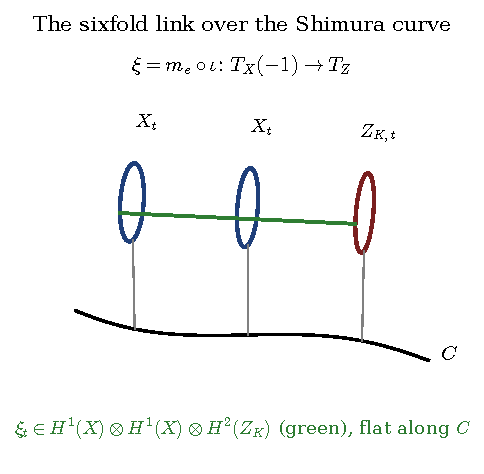
\includegraphics[width=0.78\textwidth]{figures/fig_link}
\caption{The sixfold link. Two copies of the Mumford fourfold $X_{t}$ and the sixfold $Z_{K,t}$ sit over the same point $t$ of the Shimura curve $C$; the class $\xi_{t}$ in the mixed K\"unneth component identifies the two copies of $T$ and is flat along $C$.}
\label{fig:link}
\end{figure*}

\begin{theorem}[The sixfold link]\label{thm:link}
Let $t\in C$ be a point at which $X=X_{t}$ has Hodge group $G$, and let $\xi$ be a nonzero element of $\Hom_{\Hdg}(T_{X}(-1),T_{Z})\subseteq H^{4}(X\times X\times Z_{K})$.
\begin{enumerate}[label=\textup{(\roman*)},leftmargin=2.4em,itemsep=2pt]
\item $\Hom_{\Hdg}(T_{X}(-1),T_{Z})=F\cdot\iota$ for the identification $\iota$ of Lemma~\ref{lem:tz}, so $\xi=m_{e}\circ\iota$ for a unique $e\in F^{\times}$. The $G\cdot K^{1}$-invariant classes of degree four on $X\times X\times Z_{K}$ have dimension $26$; they are Hodge classes at every $t$, when the right-cocharacter orbit has full span, at a very general $t$ they are all the Hodge classes of degree four, and there $\xi$ and $\psi\otimes\NS(Z_{K})$ are the only ones in the K\"unneth component $H^{1}(X)\otimes H^{1}(X)\otimes H^{2}(Z_{K})$.
\item If $\xi$ is algebraic, then $\xi^{\dagger}\xi$, the composite with the adjoint for the Lefschetz pairing on $X\times X$ and the intersection pairing on $Z_{K}$, is an algebraic endomorphism of $T_{X}(-1)$ equal to $m_{a(e)}$ with $a(e)=\kappa\,e^{2}c^{2}\in F$, $\kappa\in\QQ^{\times}$.
\item If $a(e)\notin\QQ$, the exceptional classes of $X\times X$ are algebraic at $t$, and so is every Hodge class on every power of $X$.
\item $a(e)\notin\QQ$ for every $e\in F^{\times}$ if and only if $K$ contains no imaginary quadratic field. If $K=F\cdot k$ with $k=\QQ(\sqrt{-d})$ and $c=f\sqrt{-d}$, then $a(e)\in\QQ$ exactly for $e\in\QQ f^{-1}$.
\item Conversely, if the exceptional classes are algebraic and some algebraic cycle on $X^{r}\times Z_{K}$ acts nonzero on $T_{Z}$, then every $\xi$ is algebraic.
\end{enumerate}
\end{theorem}

\begin{proof}
(i) The Hodge group of $X\times X\times Z_{K}$ lies in $G\cdot K^{1}$ and maps onto $\Hg(X)=G$; it acts on $T_{X}(-1)$ and on $T_{Z}$ through that image, since $K^{1}$ acts trivially on both. Both are the irreducible $G$-representation $T$ with $\End_{G}T=F$ \cite[Prop.~21.2]{BMB26}, so $\Hom_{\Hdg}=F\iota$. The count is the dimension of the kernel of the six raising and lowering operators of $\mathfrak{sl}_{2}^{3}$ on the torus-weight-zero part of $\bigwedge^{4}(V\oplus V\oplus D)$, computed by K\"unneth type: $(1,1,2)$ gives $3+3$, the line $F\iota$ and $\psi\otimes\NS(Z_{K})$; $(2,2,0)$ gives $4=\QQ\oplus F$, the Hodge classes of $X\times X$ in $H^{2}\otimes H^{2}$; $(0,0,4)$ gives $6=S^{2}\NS(Z_{K})$; $(2,0,2)$ and $(0,2,2)$ give $3$ each; and $(4,0,0)$, $(0,4,0)$, $(3,1,0)$, $(1,3,0)$ one each, products of divisor classes. The sum is $26$. The Hodge group of the product lies in $G\cdot K^{1}$, so these $26$ classes are Hodge classes at every $t$, and $26$ is a lower bound for the Hodge classes of degree four. Under the full-span hypothesis, at a very general $t$ the argument of Lemma~\ref{lem:polarisations}, applied to the family $X\times X\times Z_{K}$ over $C$, whose monodromy is again Zariski dense in $G$, gives Hodge group exactly $G\cdot K^{1}$, and then the $26$ classes are all of them; the description of the K\"unneth component $(1,1,2)$ follows.

(ii) The adjoint of a correspondence for the Lefschetz pairing on $H^{2}(X\times X)$ and the polarised intersection pairing on $Z_{K}$ is the transposed cycle composed with cup products with powers of the polarisations and the inverse Lefschetz isomorphism, which is algebraic on an abelian variety \cite[\S2]{Kle68}; so $\xi^{\dagger}\xi$ is algebraic. By Lemma~\ref{lem:tz}, $T_{X}(-1)$ carries $-4q_{1}$ and $T_{Z}$ carries a rational multiple of $q_{c^{2}}$, and for $\xi=m_{e}$, $q_{c^{2}}(m_{e}x,m_{e}y)=\Tr(c^{2}e^{2}\trd(xy))=q_{1}(c^{2}e^{2}x,y)$, so $\xi^{\dagger}\xi=\kappa\,m_{e^{2}c^{2}}$.

(iii) An irrational element of the cubic field generates $F$. The algebraic endomorphism $C=\xi^{\dagger}\xi$ is zero off the multiplicity-one adjoint summand after the degree projectors and the projector on $Z_K$ are applied. It is invertible on that summand. Polynomial interpolation in $C$ therefore gives its projector and the full $F$-action there. The tensor argument of Theorem~\ref{v7:thm:powers}, using partial symplectic transpose, then gives all Hodge classes on every power of $X$ and in particular the two exceptional directions on $X^2$. Ordinary cup product cannot be used here: the adjoint summand lies in $\operatorname{Sym}^{2}V$, whereas cup product maps to $\bigwedge^{2}V$. This distinction replaces the earlier contraction argument. Algebraicity remains a statement at the chosen fibre; no propagation to every point of $C$ follows.

(iv) $a(e)=\kappa e^{2}f^{2}\delta$ is rational iff $e^{2}f^{2}\delta\in\QQ$. If $-\delta\notin\QQ^{\times}(F^{\times})^{2}$ then $\delta\notin\QQ^{\times}(F^{\times})^{2}$ and $e^{2}f^{2}\delta\in\QQ$ is impossible. If $-\delta=-dg^{2}$ with $d\in\QQ^{\times}$, $g\in F^{\times}$, then with $c=f\sqrt{-d}$ one gets $a(e)=\kappa e^{2}f^{2}d$, rational iff $(ef)^{2}\in\QQ$ iff $ef\in\QQ$, a cubic field having no irrational element with rational square. And $-\delta\in\QQ^{\times}(F^{\times})^{2}$ exactly when $K\supseteq\QQ(\sqrt{-d})$ for some $d$.

(v) By \cite[Thm.~21.7]{BMB26} the Hodge conjecture holds for all powers of $X$ once the exceptional classes are algebraic. A cycle on $X^{r}\times Z_{K}$ acting nonzero on the irreducible $T_{Z}$ carries it isomorphically onto a summand of $H^{2k}(X^{r})(k-1)$; projecting onto that summand and composing with an isomorphism to $T_{X}(-1)\subseteq H^{2}(X\times X)$, a Hodge class on $X^{r+2}$ and algebraic, gives an algebraic nonzero element of $\Hom_{\Hdg}(T_{Z},T_{X}(-1))=F$; composing with the algebraic $m_{a}$ gives every element of that line, and transposing gives every $\xi$.
\end{proof}

\begin{proposition}[Hyper-K\"ahler carriers give $\pm1$]\label{prop:hk}
Let $Y_{1},\dots,Y_{m}$ be projective hyper-K\"ahler varieties of K3$^{[n_{j}]}$ type whose transcendental spaces are Hodge isometric to $(T,r_{j}q_{\lambda_{j}})$, $r_{j}\in\QQ^{\times}$, $\lambda_{j}\in F$ totally positive. Every composite of rational Hodge isometries between them that returns to $Y_{j}$ acts on $T$ by $\pm1$, and every composite of Hodge similarities by an element of $\QQ$.
\end{proposition}

\begin{proof}
A Hodge isometry $(T,r_{j}q_{\lambda_{j}})\to(T,r_{k}q_{\lambda_{k}})$ is a Hodge endomorphism of $T$, hence $m_{a}$ for some $a\in F$, and it is an isometry iff $r_{j}\lambda_{j}=r_{k}\lambda_{k}a^{2}$. A composite returning to $j$ is $m_{a}$ with $a^{2}=1$, and a composite of similarities is $m_{a}$ with $a^{2}\in\QQ$, which in a cubic field forces $a\in\QQ$. The isometries are algebraic by \cite{Bus19,Mar24}, which is why the statement matters: they realise $m_{b}$ between $S_{\lambda}$ and $S_{\lambda b^{-2}}$ and between their moduli spaces of sheaves, but every return is trivial.
\end{proof}

\subsection{Where the link stops}\label{ssec:f2stop2}

The algebraicity of $\xi$ at a full-group fibre remains the missing input. The CM computation must distinguish the embeddings used to define the right circle of $Z_K$. For the matched choice $K=Fk$ constructed in Sections~\ref{v7:sec:setup} and~\ref{v7:sec:seed}, the special fibre satisfies
\[
 X_c\sim E_k\times B,\qquad Z_{K,c}\sim E_k^3\times B,
\]
and the mixed class is algebraic. Thus a blanket assertion that $\Hom(X_c,Z_{K,c})=0$ at a compositum CM point is incorrect. At a full-group fibre the weight-one representations do have no common constituent and this Hom group is zero. Proposition~\ref{v7:prop:firstorder} shows that even first-order continuation of a nonzero matched CM homomorphism fails. It does not obstruct the flat degree-four class itself. The new sections construct the special cycle, its dense orbit and the precise conditional transfer to all powers; none supplies a generic algebraic cycle.

\section{The two weight-one representations}\label{v7:sec:setup}

Let \(F/\Q\) be a totally real cubic field and \(D/F\) a quaternion algebra split at one real place and ramified at the other two. Assume the split corestriction condition in Mumford's construction \cite{Mum69,vG00}. Put \(G=\Res_{F/\Q}\SL_1(D)\). After a splitting extension the eight-dimensional rational representation \(V=H^1(X,\Q)\) is \(V_1\otimes V_2\otimes V_3\), with \(V_i\) the two-dimensional standard module at the \(i\)-th embedding of \(F\). Index the split real place by 3. The Hodge circle acts through its standard circle in the third factor. A full-group fibre means that its Hodge group is the image of \(G\) in \(\operatorname{GL}(V)\); this image differs from \(G\) by a finite central kernel.

\begin{lemma}[Choice of a common quadratic field]\label{v7:lem:field}
There is an imaginary quadratic field \(k\) such that \(K=Fk\) embeds in \(D\) as a maximal commutative subfield.
\end{lemma}
\begin{proof}
For each rational prime \(p\) below a finite ramified place of \(D\), choose a quadratic field over \(\Q_p\) that does not embed in any ramified \(F_v\) above \(p\). A local degree one or three cannot contain a quadratic field. There is at most one local degree two above \(p\), since the sum of the local degrees is three. If present, it forbids only its own quadratic field. Each \(\Q_p\) has more than one quadratic field. Prescribe these finitely many local squareclasses and a negative real sign. Weak approximation gives a rational representative and hence an imaginary quadratic field \(k\) realizing them. The extension \(Fk/F\) is a field at every ramified finite place and is complex at both ramified real places. The local-global embedding criterion for a quadratic field in a quaternion algebra gives \(K\hookrightarrow D\) \cite{Reiner75}.
\end{proof}

Fix such an embedding and write \(T=\Res_{F/\Q}(\ker N_{K/F})\). The twelve-dimensional rational space \(D\) has an action of \(G\times T\) by left and right multiplication, \((g,t)x=gxt\). Choose the complex embedding of \(k\) whose circle in the embedded split-place torus lies in the chosen component of the Mumford domain. Use this embedding for the right circles at both compact places. At the third place use the varying left circle from the Mumford fourfold, with trivial right circle. The resulting complex structure \(J\) squares to \(-1\) and defines a weight-one rational Hodge structure. Right multiplication by \(K\) commutes with \(J\).

For \(c\in K\) with \(\bar c=-c\), the form
\[
 \psi_c(x,y)=\Tr_{F/\Q}\trd(\bar xyc)
\]
is alternating and invariant under \(G\times T\). Conjugation and cyclicity of reduced trace give alternation. Left multiplication by \(g\) inserts \(\bar gg=1\), and right multiplication by \(t\) gives a cyclic conjugation of \(c\) by \(t\). The form is nondegenerate for \(c\ne0\). At a compact place the evaluation on \(x,Jx\) is a nonzero scalar times the positive quaternion norm, with the sign selectable by \(c\). At the split place choose bases for the left and right imaginary units. For \(j=\left(\begin{smallmatrix}0&-1\\1&0\end{smallmatrix}\right)\) and \(Jx=jx\), the choice \(c=-j\) gives
\(\trd(\bar x(jx)(-j))=\Tr(x^{\mathsf t}x)>0\) for \(x\ne0\). Changing a local orientation changes the required sign of \(c\). By weak approximation, an element of \(k\) with \(\bar c=-c\) can be multiplied by an element of \(F^\times\) to meet the three sign requirements. Thus this rational Hodge structure is polarizable and is realized by an abelian sixfold \(Z\) up to isogeny. The right \(K\)-action is realized by rational endomorphisms of \(Z\), using the equivalence between polarizable weight-one Hodge structures and complex abelian varieties up to isogeny.

We work on the connected Shimura curve after passing to fine level and, if necessary, a finite cover on which both representations give polarized abelian schemes. In the weight-one Shimura construction the left circle varies over the Mumford domain and the right circle is fixed. One uses lattices in the two rational representations and a common congruence subgroup preserving them. The period maps to the fine moduli spaces of polarized abelian varieties give the two schemes over the curve. All the representations and splittings used below are defined over \(\Q\) before varying the circle.

\subsection{The rank-nine summands}

Over a splitting field \(D=\bigoplus_{i=1}^3 D_i\), where
\[
 D_i=V_i\otimes(W_i^+\oplus W_i^-)
\]
and \(W_i^\pm\) are inverse characters of the \(i\)-th factor of \(T\). The invariant part of \(\bigwedge^2 D\) for \(T\) is
\begin{equation}\label{v7:eq:invariants}
 (\bigwedge^2 D)^T
 = \bigoplus_i \bigl((\operatorname{Sym}^2 V_i)\oplus\Q(-1)_i\bigr)
\end{equation}
after scalar extension, where the notation for each trivial summand records its weight two. Indeed the only \(T\)-neutral wedge pairs in one block have opposite weights and the cross-block characters are nontrivial. Denote the sum of the three adjoint summands by \(T_Z\) and the remaining rank-three Tate subspace by \(L_Z\); both descend to \(\Q\).

In \(V\otimes V\), decompose each \(V_i\otimes V_i\) into its symmetric and alternating parts. The sum with one symmetric and two alternating parts is a copy \(T_X\) of the same three adjoint representations. It lies in the symmetric square of \(V\), and we view it in the mixed \(H^1\otimes H^1\) component of \(H^2(X^2)\). Each adjoint is defined at an embedding of \(F\) and the summands are transitively permuted by Galois. Thus the adjoint sum is irreducible over \(\Q\), has multiplicity one in \(V\otimes V\), and has commuting field \(F\). On \(T_Z\) the right circle acts trivially. The two Hodge structures therefore admit a rational \(G\)-equivariant identification \(\iota:T_X\to T_Z\), flat on the curve. A choice of invariant pairing on \(V\otimes V\) realizes it as a flat Hodge class \(\xi\) in the component
\[
 H^1(X,\Q)\otimes H^1(X,\Q)\otimes H^2(Z,\Q)
 \subset H^4(X^2\times Z,\Q).
\]
Every rational \(G\)-equivariant map between these adjoint summands is an element of \(F\iota\). At full-group fibres the same holds for Hodge morphisms, since their Hodge circles project to the full \(G\)-image.

\subsection{Algebraic projection on the sixfold}\label{v7:sec:projector}

\begin{proposition}\label{v7:prop:proj}
The projector onto \(T_Z\) in \eqref{v7:eq:invariants}, with zero action in other cohomological degrees, is induced by a rational algebraic correspondence. Every multiplication \(m_a\) on \(T_Z\), \(a\in F\), with zero action on its complement, is induced by a rational algebraic correspondence.
\end{proposition}
\begin{proof}
The multiplication-by-two morphism induces multiplication by \(2^j\) on \(H^j(Z)\). Polynomial interpolation in its pullback gives algebraic projectors onto the individual cohomological degrees. On \(H^2(Z)\), choose \(t\in T(\Q)\) at which no nontrivial character appearing in \(\bigwedge^2 D\) takes the value 1. Such points exist because \(T(\Q)\) is Zariski dense: the map \(a\mapsto a/\bar a\) from \(\Res_{K/\Q}\mathbb G_m\) is dominant and the source has dense rational points. The induced pullback by the rational endomorphism is algebraic on \(H^2\). Here and below rational endomorphisms act by normalizing the graphs of their integral multiples in the indicated cohomological degree. The operator is semisimple, so a polynomial with rational coefficients projects onto its eigenvalue 1 space. This gives the projector onto \((\bigwedge^2D)^T\).

The Tate subspace \(L_Z\) consists of divisor classes by Lefschetz \((1,1)\). It contains the polarization class \(\theta\) associated to \(\psi_c\). On \(H^2(Z)\), use the pairing
\(q_Z(a,b)=\int_Z a b\,\theta^4\). The restriction to \(L_Z\) is nondegenerate: the \(\theta\)-line is positive and its orthogonal complement in \(L_Z\) is negative definite by the Hodge index theorem. A divisor basis and its dual for this pairing give an algebraic projector onto \(L_Z\) via external products and multiplication by \(\theta^4\). By \(G\times T\)-invariance, \(L_Z\) is orthogonal to \(T_Z\) and to the nontrivial \(T\)-weights. Subtracting this projector gives the claimed projector onto \(T_Z\).

Right multiplication by \(u\in F^\times\) acts on \(H^1(Z)\) by \(\sigma_i(u)\) on \(D_i\). Its pullback on \(T_Z\) acts by \(m_{u^2}\). Choose \(u\notin\Q\). Its square is not rational because \(F\) has prime degree three. Consequently \(u^2\) generates \(F\). Compose with the projector and take polynomials with rational coefficients to obtain all \(m_a\).
\end{proof}

\begin{proposition}[The powers of the sixfold]\label{v7:prop:sixfold}
At a full-group Mumford fibre, the Hodge ring of each power \(Z^m\) is generated by divisor classes.
\end{proposition}
\begin{proof}
The projection of \(\Hg(Z)\) to the adjoint quotient of \(G\) is surjective, since the image of the Hodge circle there is the one for \(X\). The derived group thus contains the image of \(G\). Its torus quotient is also full. Indeed \(F\) is totally real and \(k\) is imaginary quadratic, so the Galois action on the three coordinates of \(T\) is by permutations of the embeddings and a simultaneous sign. The cocharacter of the fixed right circle is \((1,1,0)\), up to simultaneous sign. Its orbit spans \(\Q^3\), since the three vectors with one zero and two ones are independent. Modulo the finite central intersection, the Hodge group is therefore the full image of \(G\times T\).

After scalar extension, the action on the \(i\)-th block is that of \(\operatorname{GL}(V_i)\) on \(V_i\oplus V_i^\vee\). The inverse characters on \(W_i^\pm\) and the alternating form on \(V_i\) give this identification. On \(Z^m\) one has \(m\) copies of each block. In the full tensor algebra the invariants of each \(\operatorname{GL}(V_i)\) are spanned by products of evaluation pairings between a standard and a dual factor, by the first fundamental theorem of invariant theory \cite{Weyl39}. This holds independently at the three embeddings. Antisymmetrizing gives the same generation statement in exterior cohomology. Rational generation follows because scalar extension commutes with invariants and with the image of the multiplication map. Degree-two invariants are rational \((1,1)\)-classes, hence divisor classes.
\end{proof}

\section{The mixed cycle at a matched CM fibre}\label{v7:sec:seed}

\begin{theorem}\label{v7:thm:seed}
For the choice \(K=Fk\) of Lemma~\ref{v7:lem:field}, there is a CM fibre \(c\) on the Mumford curve and an elliptic curve \(E\) of CM type by \(k\) such that
\[
 X_c\sim E\times B,\qquad Z_c\sim E^3\times B,
\]
where \(B\) is an abelian threefold and \(\sim\) denotes isogeny. Every Hodge class on \(X_c^a\times Z_c^b\) is algebraic for all \(a,b\ge0\). In particular the flat class \(\xi_c\) has an algebraic representative.
\end{theorem}

\begin{proof}
Choose the CM point whose split-place left circle lies in the embedded \(K^1\). Such a circle is conjugate to the chosen split-place circle, with its sign selected to lie in the chosen connected domain. Fix the orientations at the compact places so that the right circle there uses the same embedding of \(k\). This is allowed by the polarization sign choice in Section~\ref{v7:sec:setup}.

Write the character lattice of \(T\) over a splitting field with basis \(e_1,e_2,e_3\). The Hodge circle on \(X_c\) is in the third factor. Its Galois conjugates generate \(T\), since \(F\) has three transitively permuted embeddings and \(k\) is disjoint from its totally real Galois closure. Thus the eight weights of \(H^1(X_c)\) for this Hodge torus are
\[
 \pm e_1\pm e_2\pm e_3 ,
\]
each with multiplicity one. The pair \(\pm(e_1+e_2+e_3)\) is defined over \(\Q\) as a subrepresentation because Galois acts by permutations and simultaneous sign. This pair is \(H^1(E)\), as a rational Hodge structure. The six remaining weights give \(H^1(B)\). The decomposition gives the first isogeny.

At the same point, the joint left and right torus for \(Z_c\) is the graph of the rational morphism
\[
 T\longrightarrow T,\qquad t\longmapsto N_{K/k}(t)t^{-1}.
\]
The norm has \(N_{K/k}(t)\overline{N_{K/k}(t)}=1\) because \(t\bar t=1\). Thus the displayed map takes values in \(T\). On coordinates it replaces the \(i\)-th character by the sum of the other two. It sends the left circle in the third factor to the right circle in the first two, so the Hodge circle of the pair lies in this graph. Its Galois conjugates span the graph. On \(D_i=V_i\otimes(W_i^+\oplus W_i^-)\), the resulting weights are
\[
 \pm e_i\ \pm(e_j+e_\ell),\qquad \{i,j,\ell\}=\{1,2,3\}.
\]
The two signs that agree give the elliptic pair at each \(i\). The signs that disagree give precisely the remaining six weights of \(X_c\), each once. Rational representations of a torus are determined by their characters with the Galois action. Their Hodge structures are determined here by the same circle on that torus. Consequently \(H^1(Z_c)\cong H^1(X_c)\oplus H^1(E)^{\oplus2}\) as rational Hodge structures, giving the second isogeny.

It remains to establish algebraicity on powers of \(X_c\); algebraicity in dimension four by itself does not automatically pass to powers. Represent the eight weights as \(\pm w_i\), with
\[
 w_1=(1,1,1),\quad w_2=(1,-1,-1),\quad
 w_3=(-1,1,-1),\quad w_4=(-1,-1,1).
\]
Their only rational relation, up to scalar, is \(w_1+w_2+w_3+w_4=0\). In a zero-weight multiset, first remove all opposite pairs. If \(\alpha_i,\beta_i\) were the multiplicities of \(w_i,-w_i\), then all differences \(\alpha_i-\beta_i\) are equal. The residual multiset is therefore a union of positive tetrahedra \(\{w_1,w_2,w_3,w_4\}\) or negative tetrahedra. In the exterior algebra of \(H^1(X_c^m)\), each invariant monomial factors into invariant pieces of these two types and opposite pairs.

We first realize the two tetrahedra on the fourfold. The four \(w_i\) are stable under permutation of the coordinates and are exchanged with the four \(-w_i\) by simultaneous sign reversal. Define a rational \(k\)-action by \(\alpha\) on the \(w_i\) and by \(\bar\alpha\) on the \(-w_i\), for \(\alpha\in k\). The Galois description shows descent, and the action preserves the Hodge decomposition. Each embedding has two weights in \(H^{1,0}\), since the split coordinate takes the positive sign on exactly two of the four weights in each set. This is a Weil-type action, and its two determinant lines are precisely the two tetrahedra.

The isogeny \(X_c\sim E\times B\) is compatible with this action, with \(E\) of \(k\)-rank one. Choose a \(k\)-compatible rational product polarization. Such a polarization can be obtained on each factor by replacing an alternating polarization form \(\psi\) by
\(\psi(x,y)+d^{-1}\psi(Ix,Iy)\), where \(I\) is the action of \(\sqrt{-d}\). This is a positive sum of polarizations and satisfies \(\psi'(Ix,Iy)=d\psi'(x,y)\). Let \(\delta\in\Q^\times\) be the determinant of the associated \(k\)-Hermitian form in a \(k\)-basis adapted to the product. Its signature is \((2,2)\), so \(\delta>0\). Multiplying the polarization on \(E\) by \(\delta^{-1}\) preserves positivity and changes the determinant by \(\delta^{-1}\). Clearing denominators of the resulting rational polarization changes the determinant by a rational fourth power, a norm from \(k\). The discriminant is therefore one. Markman's theorem on discriminant-one Weil fourfolds \cite[Theorem 1.5]{Mar23} gives algebraicity of the rational determinant space, and hence of both tetrahedra after extending coefficients. Lefschetz \((1,1)\) gives algebraicity of the opposite pairs.

We explain why the pieces on a power come from the fourfold. Over a splitting field the commuting algebra \(\End_{\mathrm{HS}}(H^1(X_c))\) is the full diagonal algebra on the eight one-dimensional weight spaces, since the weights are distinct. Its rational part is the algebra of rational abelian endomorphisms. For a homomorphism \(X_c^m\to X_c\) up to rational multiples, the pullback on \(H^1\) is given by \(m\) commuting endomorphisms. Over a splitting field their diagonal entries can be chosen independently at each weight. Thus the pullbacks of a pair or tetrahedron on \(X_c\) span every corresponding piece with arbitrary multiplicity slots on \(X_c^m\). These pullbacks are spanned by pullbacks by rational homomorphisms after extending scalars: if a linear functional kills all rational evaluations, it kills the polynomial in the endomorphism parameters identically, because rational points of the parameter vector space are Zariski dense. Hence the pieces and their products are algebraic over the splitting field. Faithfully extending scalars in the rational cycle class map shows algebraicity over \(\Q\).

Finally \(X_c^a\times Z_c^b\) is an isogeny summand of a power of \(X_c\). Indeed \(E\) is an isogeny factor of \(X_c\), and \(Z_c\sim X_c\times E^2\). There are rational homomorphisms to and from a sufficiently large power with composite the identity on the summand. Pull a Hodge class up from the summand to that power, represent it by an algebraic class there, and pull back along the other homomorphism. Clearing denominators gives the required rational algebraic class.
\end{proof}

\begin{remark}
The construction uses the discriminant-one theorem at the CM seed and then elementary weight generation. At the matched seed the homomorphisms between \(X_c\) and \(Z_c\) are nonzero. The vanishing of those homomorphisms at full-group fibres does not extend to this CM point.
\end{remark}

\section{What one algebraic link gives at a full-group fibre}\label{v7:sec:transfer}

Fix a full-group fibre and use \(X,Z,T_X,T_Z\) for its data. Write \(\theta_X,\theta_Z\) for polarizations. At this fibre \(T_X\) and \(T_Z\) are irreducible Hodge structures, and \(\End_{\mathrm{HS}}(T_X)=\End_{\mathrm{HS}}(T_Z)=F\). In particular they have no rational Tate summand and the relevant Lefschetz pairings are nondegenerate on them.

\begin{proposition}[Transfer of the cubic action]\label{v7:prop:transfer}
If an algebraic correspondence \(X^2\to Z\) induces a nonzero map from \(T_X\) to \(T_Z\) after projection to the indicated cohomological components, then the projector onto \(T_X\) and the action of \(F\) on it are algebraic. This criterion holds for the compositum field used at the CM seed.
\end{proposition}
\begin{proof}
Use the algebraic \(H^1\otimes H^1\) projector on \(X^2\) and the projector of Proposition~\ref{v7:prop:proj} on \(Z\). By multiplicity one, the resulting operator \(f\) vanishes off \(T_X\) in \(H^1\otimes H^1\) and is an isomorphism \(T_X\to T_Z\). An algebraic representative of \(\xi\) would give such an operator by multiplication with a power of the polarization on the source and pushforward.

Use the nondegenerate pairings on degree two given by cup product with the appropriate powers of the polarizations. The adjoint \(f^\dagger\) is algebraic: transpose the cycle and use multiplication by these powers and the inverse Lefschetz isomorphism, which is algebraic for abelian varieties \cite{Kle68}. Put \(C=f^\dagger f\). It is zero off \(T_X\) and invertible on \(T_X\). If \(g(t)\) is the minimal polynomial of its restriction to \(T_X\), then \(g(0)\ne0\). The Chinese remainder theorem supplies a polynomial \(P(t)\) with \(P(0)=0\) and \(tP(t)\equiv1\bmod g(t)\). Hence \(P(C)C\) is the projector onto \(T_X\), and
\[
 P(C)\,f^\dagger m_a f
\]
is multiplication by \(a\) on \(T_X\) and zero off it, where \(m_a\) on \(T_Z\) is algebraic by Proposition~\ref{v7:prop:proj}. The identification of the field actions follows from \(f\in F\iota\). If \(f=m_e\iota\), then \(m_{e^{-1}}f=\iota\) is itself algebraic. Applying the inverse Lefschetz map on the source factor to its correspondence class recovers \(\xi\). This uses no nonsquare condition on the polarization or the chosen extension \(K/F\).
\end{proof}

\subsection{From the cubic action to all powers}

We use the following tensor conventions. The polarization gives an alternating form \(\psi\) on \(V\). It and its inverse tensor are algebraic operations: one contracts two \(H^1\) factors by pulling back along a diagonal, multiplying by a polarization power and integrating, and the inverse tensor is a rational multiple of the corresponding mixed Poincar\'e class. Factor permutations and the \(H^1\) K\"unneth projectors are algebraic. Thus a correspondence on \(V\otimes V\) can be treated as an algebraic tensor on four factors, and permutations of its slots, including the partial symplectic transpose, are again algebraic. These assertions may also be obtained by using the algebraic inverse Lefschetz maps of the abelian variety to convert its dual \(H^1\) factors.

\begin{theorem}\label{v7:thm:powers}
At a full-group fibre, an algebraic projector onto \(T_X\) together with its algebraic \(F\)-action implies the rational Hodge conjecture on every \(X^m\). Thus the hypothesis of Proposition~\ref{v7:prop:transfer} implies the conjecture for all such powers.
\end{theorem}
\begin{proof}
Extend coefficients to a splitting field for the representation and the three embeddings of \(F\). Write \(s_i\) for the operator that swaps the two copies of \(V_i\) in \(V\otimes V\) while leaving the other factors fixed, and set \(p_i=(1-s_i)/2\). The three field projectors on \(T_X\), obtained by interpolation in a cubic generator, act on \(V\otimes V\) as
\[
 P_i=(1-p_i)p_jp_\ell,\qquad \{i,j,\ell\}=\{1,2,3\}.
\]
They are algebraic by hypothesis. Let \(\tau\) denote symplectic transpose in the first \(V\) slot, leaving the second slot fixed. The form \(\psi\) is proportional to the product of the three alternating forms. On a two-dimensional factor, partial symplectic transpose sends the swap \(s\) to \(1-s\). Indeed ordinary partial transpose of the swap is the rank-one operator with tensor \(e_1\otimes e_1+e_2\otimes e_2\) on both sides. Conjugation in the first slot by the alternating matrix changes this to the projector times two onto \(e_1\otimes e_2-e_2\otimes e_1\). Therefore \(\tau(p_i)=s_i/2\). Transpose factors independently for this product, giving
\[
 \tau(P_i)=(1-s_i/2)(s_j/2)(s_\ell/2).
\]
The \(s_i\) commute and have eigenvalues \(+1,-1\). The square of the last expression equals \(1/64\) on the \(+1\) eigenspace of \(s_i\) and \(9/64\) on its \(-1\) eigenspace. Hence
\[
 p_i=\frac{64\,\tau(P_i)^2-1}{8}.
\]
This realizes each individual swap \(s_i\) algebraically on the whole \(V\otimes V\). Here the identity is on \(V\otimes V\), enforced by the degree projectors.

On \(V^{\otimes 2d}\), apply a swap to adjacent \(V\) slots to permute the \(i\)-th standard factors independently for each \(i\). The invariants in \((V_i)^{\otimes 2d}\) are spanned by tensors pairing the slots in twos with the alternating form \cite{Weyl39}. In odd degree there are no invariants. Start with \(d\) copies of the algebraic inverse tensor of \(\psi\), which supplies the same pairing in all three colors. Independent permutations give all triples of pairings. Hence every invariant tensor in \(V^{\otimes 2d}\) is algebraic over the splitting field. Passing to exterior cohomology on \(X^m\) is algebraic: choose the slots for each of the \(m\) factors and use diagonal pullback and cup product. The maps span the invariant exterior algebra since antisymmetrization is equivariant in characteristic zero. Rational algebraicity follows by scalar descent.
\end{proof}

\subsection{The two classes on the square}

\begin{proposition}\label{v7:prop:square}
At a full-group fibre, \(\dim_\Q \Hdg^2(X^2)=8\) and products of divisors span a six-dimensional subspace. Any single algebraic class outside that span implies algebraicity of both exceptional directions and the Hodge conjecture on every power of \(X\).
\end{proposition}
\begin{proof}
The primitive part \(U\) of \(\bigwedge^2 V\) has three irreducible complex summands, each with one alternating and two symmetric factors in \(V\otimes V\). The remaining summand, with three alternating factors, is the polarization line. Thus \(\End_{\mathrm{HS}}(\bigwedge^2 V)=\Q\oplus F\). The invariants in \(H^4(X^2)\) in K\"unneth bidegrees \((4,0),(3,1),(2,2),(1,3),(0,4)\) have dimensions \(1,1,4,1,1\). For the middle bidegree use the endomorphism computation. For the others, the trivial representation in \(\bigwedge^4 V\) and the copy of \(V\) in \(\bigwedge^3 V\) each have multiplicity one. To see this last count, the weights of \(V\) are the eight sign triples. Count subsets of size four with sum equal to a specified tuple having \(j\) coordinates equal to 2 and the others 0. The counts for \(j=0,1,2,3\) are \(8,4,2,1\). For size three, count tuples with \(j\) coordinates equal to 3 and the others 1, giving \(4,1,0,0\). Subtracting raised weights in each \(\SL_2\) coordinate gives \(8-3\cdot4+3\cdot2-1=1\) and \(4-3\cdot1=1\).

There are three divisor generators on \(X^2\): the two polarizations \(\theta_1,\theta_2\) and the mixed Poincar\'e divisor \(\delta\). Their six quadratic products are independent. The four nonmiddle bidegrees each receive a nonzero product: for the odd bidegrees this follows by hard Lefschetz, or directly by multiplying the pairing tensor by a polarization. In bidegree \((2,2)\), \(\theta_1\theta_2\) is rank one and \(\delta^2\) induces, up to a scalar, the perfect pairing from the second exterior power. On the primitive space this pairing and the Lefschetz pairing are proportional, since they are invariant for \(\operatorname{Sp}(V,\psi)\), under which the primitive second exterior power is irreducible. The exceptional quotient is thus \(F/\Q\) in the primitive endomorphism space.

Project an algebraic class outside the divisor span to bidegree \((2,2)\) and then to \(U\) on both sides, using degree projectors and subtraction of the polarization line. Conversion to an endomorphism by the algebraic Lefschetz maps gives multiplication by an element of \(F\setminus\Q\). Since \(F\) is cubic, its powers generate the whole field. This already realizes both exceptional directions.

For the assertion about all powers, lift the three spectral projectors of this field action into \(V\otimes V\) by pullback under the addition map and projection to \(H^1\otimes H^1\). Addition sends \(v\wedge w\) to \(v\otimes w-w\otimes v\) in that component; the exterior projection and its normalization are algebraic. These projectors act as \(p_i(1-p_j)(1-p_\ell)\). Their partial symplectic transposes are
\[
 (s_i/2)(1-s_j/2)(1-s_\ell/2).
\]
The second and third factors are strictly positive on each joint eigenspace. Polynomial interpolation taking the value 1 on negative eigenvalues and 0 on positive eigenvalues therefore recovers \(p_i\). The independent swaps then give all invariants by the argument of Theorem~\ref{v7:thm:powers}.
\end{proof}

\section{From the CM fibre to the algebraic locus}\label{v7:sec:locus}

\begin{lemma}[Strata of algebraicity]\label{v7:lem:locus}
Let \(f:\mathcal Y\to S\) be smooth and projective over a smooth connected complex algebraic variety, and let \(\gamma\) be a flat rational Hodge class in \(R^{2p}f_*\Q\). The locus \(\Sigma(\gamma)\) where \(\gamma\) is algebraic is a countable union of Zariski closed subsets. It is either all of \(S\) or meagre in the analytic topology.
\end{lemma}
\begin{proof}
For a fixed tuple of Hilbert polynomials, take the product over \(S\) of the corresponding relative Hilbert schemes. It is projective over \(S\). For a fixed tuple of rational coefficients, the condition that the indicated combination of cycle classes equals \(\gamma\) is constant on each connected component: classes of flat families of cycles give flat sections of the pulled back local system. The images of the components satisfying this condition are Zariski closed by properness. Varying the tuples enumerates the rational algebraic representatives. Proper closed subvarieties are nowhere dense in the analytic topology, so the countable union is meagre unless one image is all of \(S\).
\end{proof}

\begin{corollary}[Dense algebraic locus of the mixed link]\label{v7:cor:dense}
In the family of Section~\ref{v7:sec:setup} with its compositum field, \(\Sigma(\xi)\) is dense in the analytic topology. Either \(\Sigma(\xi)\) is the entire curve or it is a countable set.
\end{corollary}
\begin{proof}
The rational \(G\)-action on the period domain carries the special fibre of Theorem~\ref{v7:thm:seed} to isogenous pairs and transports the \(G\)-invariant class \(\xi\). Isogeny pullback and pushforward preserve algebraicity with rational coefficients, so its orbit consists of points of \(\Sigma(\xi)\). The norm-one group has rational points dense in the identity component of its real points. One sees this by the Cayley transform \(x\mapsto (1+x)(1-x)^{-1}\) of the reduced trace-zero subspace, defined over \(F\), which supplies a rational chart about the identity. Rational points of the chart are dense in a real neighbourhood of the identity, and the closed subgroup containing that neighbourhood contains the identity component. The identity component acts transitively on the connected period domain. Passing to the curve yields density. By Lemma~\ref{v7:lem:locus}, a proper \(\Sigma(\xi)\) is a countable union of proper closed subsets of a curve, hence is countable.
\end{proof}

\begin{proposition}[A sufficient bounded-degree condition]\label{v7:prop:bound}
Fix a relatively very ample line bundle on \(\mathcal Y=\mathcal X^2\times_S\mathcal Z\). Suppose that, at infinitely many distinct fibres of the Shimura curve \(S\), \(\xi\) lies in the rational span of codimension-two subvarieties of degree at most one fixed integer \(D_0\). Then \(\xi\) is algebraic at every fibre. No bound on the denominators of the coefficients is needed.
\end{proposition}
\begin{proof}
Let \(b=\dim_\Q H^4(\mathcal Y_s,\Q)\). At each of the chosen fibres, a spanning collection for \(\xi\) can be reduced to at most \(b\) classes. Parameterize ordered tuples of at most \(b\) effective cycles, each of degree in \(\{1,\ldots,D_0\}\), by the corresponding products of relative Chow varieties. These parameter spaces are proper over \(S\) and have finitely many components \cite{Ful98}. On each connected component the span of the classes is flat, so containing the fixed flat class \(\xi\) is a componentwise condition. The images of the admissible components are therefore a finite collection of closed subsets of \(S\). They contain the infinitely many chosen fibres, so one of the images is all of \(S\). This gives the claim. The span condition uses only the classes of the supports and places no restriction on rational coefficients.
\end{proof}

\subsection{The missing deformation}

The dense orbit in Corollary~\ref{v7:cor:dense} gives no uniform bound of the kind in Proposition~\ref{v7:prop:bound}. At full-group fibres, the joint Hodge group has derived group the common image of \(G\), since it projects onto the Hodge group of \(X\) and the two representations use the same left circle. The \(G\)-representations \(H^1(X)\) and \(H^1(Z)\) have no common irreducible summand. The first has the tensor product of all three standard factors and the second has only single standard factors. Therefore
\[
 \Hom(X,Z)\otimes\Q=0
\]
at such fibres. The isogeny retraction used to build the cycle at \(c\) cannot be used as a family of homomorphisms through a full-group fibre.

This also identifies a limit of the divisor construction. When the cross homomorphisms vanish, the divisors of \(X^2\times Z\) are sums of classes from \(X^2\) and from \(Z\). A product of divisors in the mixed K\"unneth component \(H^1(X)\otimes H^1(X)\otimes H^2(Z)\) has its first two factors in the span of the Poincar\'e tensor. That span is the trivial representation and is disjoint from \(T_X\). Thus divisor products cannot supply \(\xi\) on a full-group fibre even though divisors suffice on every power of \(Z\).

\subsection{The first infinitesimal test}\label{v7:sec:firstorder}

\begin{proposition}\label{v7:prop:firstorder}
At the matched CM fibre, no nonzero rational homomorphism \(X_c\to Z_c\), or \(Z_c\to X_c\), extends as a flat Hodge morphism over the first-order deformation in the nonzero tangent direction of the Shimura curve.
\end{proposition}
\begin{proof}
Work over an algebraic splitting field for the torus at \(c\). Its action on the pair is the graph torus of Theorem~\ref{v7:thm:seed}. A rational Hodge morphism \(f:H^1(X_c)\to H^1(Z_c)\) commutes with that torus. The infinitesimal period map for the varying left circle is a nonzero element \(N_3\) of the negative root line in the third \(\mathfrak{sl}_2\) factor. It has Hodge type \((-1,1)\) on both weight-one representations. On \(D_1,D_2\) its action is zero, and on \(D_3\) it is the left lower-root action.

Extending \(f\) as a flat Hodge morphism to the first-order deformation requires \([N_3,f]=0\) on \(H^{1,0}\). This commutator has type \((-1,1)\), so it is already zero on \(H^{0,1}\), whose image would have type \((-1,2)\). Thus \(f\) intertwines the entire root line. Since \(f\) is rational, it intertwines every Galois conjugate of the line. The embeddings of \(F\) are transitive, and conjugation in the common imaginary quadratic field reverses all root signs. These conjugates are the six root lines \(\pm2e_i\); they generate \(\operatorname{Lie}(G)\). It follows that \(f\) intertwines \(G\). But \(V_1\otimes V_2\otimes V_3\) and the sum of the single-standard representations \(D_i\) have no common constituent, so \(f=0\). The argument in the reverse direction is identical.
\end{proof}

The proposition concerns the weight-one morphisms used in the construction. It does not give a first-order obstruction to the final degree-four class \(\xi\), which is flat and of Hodge type along the curve.

\subsection{Representatives and semiregularity}

The companion preprint \cite{BBsecant26} studies a route using semiregularity of a perfect complex to spread a Chern character. The theorem identifies the image under semiregularity of an obstruction with the obstruction to preserving the Chern character as a Hodge class \cite{Pri24}. When the character stays Hodge, the obstruction is therefore in the kernel. Its vanishing requires an additional condition on the representative, such as injectivity of the semiregularity map. An algebraic class at the CM fibre gives a rational \(K\)-theory class, but it does not determine these self-extension groups.

\begin{proposition}[A representative with pure Chern character]\label{v7:prop:adams}
There is a perfect complex \(E\) on \(Y_c=X_c^2\times Z_c\) and an integer \(N>0\) with
\[
 \operatorname{ch}_2(E)=N\xi_c,\qquad
 \operatorname{ch}_j(E)=0\quad(j\ne2)
\]
in rational cohomology. All the components of this Chern character extend as flat Hodge classes along the curve.
\end{proposition}
\begin{proof}
Choose a rational codimension-two cycle representing \(\xi_c\) by Theorem~\ref{v7:thm:seed}. Taking the same rational combination of its structure sheaves gives a class \(v\in K_0(Y_c)_\Q\) with \(\operatorname{ch}_2(v)=\xi_c\). The second Adams operation \(\Psi^2\) satisfies \(\operatorname{ch}_j(\Psi^2v)=2^j\operatorname{ch}_j(v)\) \cite{Ful98}. Since \(\dim Y_c=14\), apply the rational polynomial operator
\[
 e_2=\prod_{\substack{0\le j\le14\\j\ne2}}
              \frac{\Psi^2-2^j}{4-2^j}.
\]
On the \(j\)-th component of the Chern character it acts as the indicator of \(j=2\). Clear denominators in \(e_2v\), and write the resulting integral \(K_0\) class as a difference of vector bundles, represented by a perfect complex. Its cohomological character is the displayed one. The nonzero component extends by \(N\xi\) and the remaining components extend by zero.
\end{proof}

This constructs the character without a deformation estimate for its representative. In the first-order direction with Kodaira--Spencer class \(\kappa\), the obstruction is the contraction of the Atiyah class with \(\kappa\), in \(\operatorname{Ext}^2(E,E)\). Its semiregularity image vanishes because the full Chern character stays Hodge. The calculation therefore requires vanishing of the obstruction inside the kernel, or injectivity on the obstruction classes, rather than only preservation of the character.

\begin{lemma}[Direct sums and the trace map]\label{v7:lem:directsum}
Let \(E_1,E_2\) be perfect complexes on a smooth projective variety. The semiregularity map of \(E_1\oplus E_2\) vanishes on the two off-diagonal summands
\(\operatorname{Ext}^2(E_1,E_2)\) and \(\operatorname{Ext}^2(E_2,E_1)\).
For \(E\oplus E\), its kernel contains
\(\operatorname{Ext}^2(E,E)\otimes\mathfrak{sl}_2\).
\end{lemma}
\begin{proof}
The Atiyah class of a direct sum is block diagonal. Each component of the semiregularity map is the trace of the product of a self-extension with a power of that class. Multiplying by an off-diagonal matrix leaves it off diagonal, with trace zero. For two identical summands the formula is the semiregularity map on \(E\) multiplied by the ordinary matrix trace, proving the second assertion.
\end{proof}

In particular \(L\oplus L\) is not semiregular on an abelian variety of dimension at least two, since \(\operatorname{Ext}^2(L,L)=H^2(\mathcal O)\ne0\). Direct sums of known objects therefore do not provide injectivity by formal additivity. A cone changes the extension groups and the differential of the complex. Its Chern character is additive, while the required deformation calculation depends on that differential.

For the mixed link it would suffice to construct a representative at \(c\) whose relative deformation space dominates the curve and whose entire Chern character remains Hodge. A dominating family gives algebraicity on an open set and Lemma~\ref{v7:lem:locus} then gives it everywhere. Neither such a representative nor the bounded-degree input is established here.

These results prove the seed statement and the algebraicity statements for the sixfold. They reduce the Mumford-square problem at a full-group fibre to a specific mixed cycle or one exceptional cycle on the square. Even a proof of that Mumford-square statement would address only one part of \(\Ftwo\). The statement \(\Fthree\) for arbitrary nonabelian varieties requires separate algebraic correspondences. The two universal statements, and hence the full Hodge conjecture, remain open.

\section{Algebraic transfer and an obstructed representative}\label{sec:v7-bypass}

The statements \Fii{} and \Fiii{} impose different requirements on a Hodge
class.  The first asks for a cycle on an abelian variety.  The second asks
for an algebraic correspondence from an abelian variety.  We record the
logical implications precisely, and then give an explicit obstruction to
deducing deformation of a chosen representative from its Chern character.

\subsection{Absolute Hodge classes and algebraic transfer}

Let $Y$ be smooth and projective over $\CC$.  The form of \Fiii{} used here
means that every $\alpha\in\Hdg^p(Y)$ has an expression
\begin{equation}\label{v7:transfer-expression}
 \alpha=\sum_{i=1}^{r}(\Gamma_i)_*\beta_i,
 \qquad
 \beta_i\in\Hdg^{q_i}(A_i),\quad
 \Gamma_i\in\operatorname{CH}^{\dim A_i+p-q_i}(A_i\times Y)_{\QQ},
\end{equation}
where the $A_i$ are complex abelian varieties.  A point is allowed as an
abelian variety of dimension zero.  The action of a correspondence is
\[
 (\Gamma_i)_*\beta_i
   =(\operatorname{pr}_Y)_*
       \bigl(\operatorname{pr}_{A_i}^*\beta_i\cup[\Gamma_i]\bigr).
\]

\begin{proposition}\label{v7:absolute-transfer}
If $Y$ satisfies \Fiii{}, every rational Hodge class on $Y$ is an absolute
Hodge class.  Consequently the universal statement \Fiii{} implies the
absolute Hodge conjecture for all smooth projective complex varieties.
\end{proposition}

\begin{proof}
Use an expression \eqref{v7:transfer-expression}.  Deligne's theorem
\cite[Theorem~2.11]{Del82} makes every $\beta_i$ an absolute Hodge class.
Cycle classes of algebraic correspondences are absolute Hodge, and
pullback, cup product and proper pushforward preserve absolute Hodge
classes.  To see the last assertion directly, spread the finitely many
varieties and correspondences over one subfield of $\CC$ of finite
transcendence degree.  Under every embedding of that field into $\CC$,
comparison and base change identify the displayed correspondence action
with the action of the conjugate algebraic correspondence.  Its source
class remains rational and of Hodge type by Deligne's theorem.  Its image
therefore remains rational and of Hodge type with the indicated Tate
twist.  Finite sums have the same property, so $\alpha$ is absolute Hodge.
\end{proof}

\begin{proposition}\label{v7:equivalence-and-divisors}
The rational Hodge conjecture for all smooth projective complex varieties
is equivalent to the conjunction of the universal statements \Fii{} and
\Fiii{}.  For a fixed $Y$, the following two conditions are equivalent.
\begin{enumerate}
\item Every rational Hodge class on $Y$ is algebraic.
\item Every rational Hodge class on $Y$ admits
  \eqref{v7:transfer-expression} with each $\beta_i$ in the algebra
  generated by divisor classes on $A_i$.
\end{enumerate}
The second condition has the same force if ``in the algebra generated by
divisor classes'' is replaced by ``algebraic.''
\end{proposition}

\begin{proof}
Assume \Fii{} and \Fiii{}, and write a Hodge class as in
\eqref{v7:transfer-expression}.  By \Fii{} choose cycles $z_i$ with
$[z_i]=\beta_i$.  Compatibility of the cycle class map with intersection
and proper pushforward gives
\[
 \alpha=
 \left[\sum_i(\operatorname{pr}_Y)_*
    \bigl(\operatorname{pr}_{A_i}^*z_i\cdot\Gamma_i\bigr)\right].
\]
This proves the rational Hodge conjecture.  Conversely that conjecture
includes \Fii{}.  If $\alpha=[z]$ on $Y$, take the source to be a point,
$\beta=1$ and the correspondence to be $z$.  This proves \Fiii{}.

For the fixed-variety assertion, a polynomial in divisor classes is the
class of the same polynomial in divisor cycles.  The preceding
pushforward formula proves that condition~2 implies condition~1, and
also proves the variant with algebraic source classes.  For the converse
one can again use a point.  If a positive-dimensional source is required,
fix an elliptic curve $A$, a point $a\in A$ and a cycle $z$ representing
$\alpha$.  Then $\beta=[a]\in\Hdg^1(A)$ is a divisor class and the
correspondence $A\times z$ satisfies
$(A\times z)_*[a]=[z]=\alpha$.  Thus the divisor-source formulation
already has exactly the force of the rational Hodge conjecture on $Y$.
\end{proof}

For each abelian variety $A$, statement \Fiii{} itself holds by the
diagonal correspondence, taking the source class to be the given Hodge
class on $A$.  Thus this special case supplies no algebraic
representative of that source class.  Proposition~\ref{v7:absolute-transfer}
also supplies absoluteness without an algebraic representative.  These
are the precise conclusions available from Deligne's theorem and
algebraic transfer.

\subsection{A polystable bundle whose full character stays Hodge}

For a perfect complex $E$ on a smooth projective variety $S$, its
first-order obstruction along a deformation with Kodaira--Spencer class
$\kappa\in H^1(S,T_S)$ is
\begin{equation}\label{v7:atiyah-obstruction}
 o_{\kappa}(E)=\kappa\lrcorner\operatorname{At}(E)
       \in\Ext^2(E,E).
\end{equation}
We use the common normalization in which the Atiyah class of a line
bundle is its first Chern class.  Changing the convention changes the
formula by a common nonzero scalar or sign and preserves its vanishing.
For a line bundle $M$, the obstruction is therefore
$\kappa\lrcorner c_1(M)\in H^2(S,\mathcal O_S)$.
This formula can also be obtained from its Atiyah extension
\[
 0\longrightarrow\mathcal O_S
  \longrightarrow\mathcal D^1(M)
  \longrightarrow T_S\longrightarrow0.
\]
The connecting map on $H^1(T_S)$ is contraction with the extension
class $c_1(M)$ and measures the failure of the transition functions of
$M$ to lift over the prescribed deformation of $S$.

\begin{theorem}\label{v7:k3-obstructed-bundle}
There exist a smooth quartic K3 surface $S$, its hyperplane polarization
$H$, an $H$-polystable rank-two vector bundle $E$, and an $H$-polarized
first-order deformation $S_{\varepsilon}$ over
$\CC[\varepsilon]/(\varepsilon^2)$ with the following properties.
\begin{enumerate}
\item If $\eta\in H^4(S,\QQ)$ is the class of a point, then
  $\ch(E)=2-36\eta$.  Every component of this character extends as a
  flat Hodge class over the whole local polarized K3 deformation space.
\item The bundle $E$, viewed as a perfect complex, has no deformation
  to $S_{\varepsilon}$.
\item There are identifications
  \[
   \Ext^2(E,E)\cong\CC\oplus\CC,
   \qquad
   \sigma_E(a,b)=a+b,
  \]
  where $\sigma_E$ is the semiregularity map.  Its one-dimensional
  kernel contains the nonzero obstruction to this first-order lift.
\end{enumerate}
\end{theorem}

\begin{proof}
One explicit surface is the Fermat quartic
\[
 S=\{x_0^4+x_1^4+x_2^4+x_3^4=0\}\subset\mathbb P^3_{\CC}.
\]
Its partial derivatives have no common projective zero, so it is smooth.
Choose $a,b\in\CC$ with $a^4=b^4=-1$.  The equations
$x_0=ax_1$ and $x_2=bx_3$ define a line $\ell\subset S$.
Adjunction gives $K_S\cong\mathcal O_S$, and the hypersurface sequence
gives $H^1(S,\mathcal O_S)=0$, so $S$ is a K3 surface.
Write $H=c_1(\mathcal O_S(1))$.  Its intersection numbers are
\[
 H^2=4,\qquad H\cdot\ell=1,\qquad\ell^2=-2.
\]
The last equality follows by adjunction on the rational curve $\ell$.
Put
\begin{equation}\label{v7:k3-line-class}
 l=4[\ell]-H,\qquad L=\mathcal O_S(4\ell-H),\qquad
 E=L\oplus L^{-1}.
\end{equation}
Then
\begin{equation}\label{v7:k3-intersections}
 H\cdot l=0,\qquad l^2=-36\eta.
\end{equation}
In particular $l\ne0$, and it is independent of $H$.
Every line bundle is slope-stable.  The two summands of $E$ both have
$H$-slope zero, so $E$ is $H$-polystable.  No assertion about the Picard
number of $S$ is needed.

On a surface the Chern character has only three components, and
\[
 \ch(E)=\exp(l)+\exp(-l)=2+l^2=2-36\eta.
\]
The unit in $H^0$ and the normalized point class in $H^4$ are flat
Hodge classes in every local smooth deformation.  This proves the
first assertion.

We choose a polarized tangent direction that does not preserve $l$.
Contraction followed by cup product is the perfect Serre-duality pairing
\[
 H^1(S,T_S)\times H^1(S,\Omega_S^1)
       \longrightarrow H^2(S,\mathcal O_S)\cong\CC,
\]
using $K_S\cong\mathcal O_S$.  Since $H$ and $l$ are independent, there
is a $\kappa\in H^1(S,T_S)$ such that
\begin{equation}\label{v7:k3-tangent}
 \kappa\lrcorner H=0,\qquad
 u:=\kappa\lrcorner l\ne0.
\end{equation}
The first equation says that this is a tangent direction to polarized
deformations.  Local Torelli for K3 surfaces \cite[Theorem~5.7]{LP80} identifies their smooth
local polarized deformation space with an open subset of the period
quadric in $H^{\perp}$.  The extra condition that $l$ stay of type
$(1,1)$ is the additional period hyperplane $l^{\perp}$.
It is a proper hyperplane here.  Indeed $l$ itself represents a tangent
vector to the polarized period quadric at $H^{2,0}(S)$, and the derivative
of the defining equation of $l^{\perp}$ on that vector is $l^2=-36$.
Thus directions satisfying \eqref{v7:k3-tangent} occur in actual local
polarized deformations.  Restrict one to the first infinitesimal
neighbourhood of its central point to obtain $S_{\varepsilon}$.

The Atiyah class of a direct sum is block diagonal, and
$\operatorname{At}(L^{-1})=-\operatorname{At}(L)$.  Consequently
\eqref{v7:atiyah-obstruction} gives
\begin{equation}\label{v7:k3-obstruction-matrix}
 o_{\kappa}(E)=
 \begin{pmatrix}u&0\\0&-u\end{pmatrix}\ne0.
\end{equation}
Nonvanishing is meant in the direct-sum decomposition of
$\Ext^2(E,E)$, so deformation of the splitting is not assumed.
The obstruction class rules out a lift of the object $E$ itself,
including a lift as a perfect complex.

For completeness we compute the whole obstruction space.  Each diagonal
summand is
$\Ext^2(L,L)=\Ext^2(L^{-1},L^{-1})=H^2(S,\mathcal O_S)\cong\CC$.
Moreover $H^0(S,L^2)=H^0(S,L^{-2})=0$.  A nonzero section of either
bundle would define a nonzero effective divisor of $H$-degree zero,
contradicting ampleness.  A section without zeros would trivialize that
bundle, contradicting $l^2\ne0$.  Serre duality therefore gives
\[
 \Ext^2(L,L^{-1})=H^2(S,L^{-2})=0,
 \qquad
 \Ext^2(L^{-1},L)=H^2(S,L^2)=0.
\]
On a surface the semiregularity target has only its degree-zero Atiyah
component, because $H^{q+2}(S,\Omega_S^q)=0$ for $q>0$.
Thus $\sigma_E$ is the ordinary trace to $H^2(S,\mathcal O_S)$,
which is $(a,b)\mapsto a+b$ in the displayed decomposition.
Its kernel is the anti-diagonal, containing the nonzero class $(u,-u)$
of \eqref{v7:k3-obstruction-matrix}.  Each line-bundle summand separately
has an isomorphism as its semiregularity map.
\end{proof}

All components of the character in Theorem~\ref{v7:k3-obstructed-bundle}
are already algebraic.  The failure concerns the lift of this particular
polystable representative.  The example proves that preserving an entire
Chern character, including the determinant, does not force a chosen
perfect complex to deform.  It also proves that injective semiregularity
of the summands does not imply injective semiregularity of their sum.

\subsection{The remaining requirement for a pure character}

For a general perfect complex, the Atiyah--Kodaira--Spencer obstruction is described in \cite{HT10}; the components of semiregularity have
the form
\[
 \sigma_{E,q}(a)=\frac{1}{q!}
    \operatorname{tr}\bigl(a\operatorname{At}(E)^q\bigr)
       \in H^{q+2}(Y,\Omega_Y^q).
\]
With the signs and normalization of \eqref{v7:atiyah-obstruction},
compatibility with first-order variation gives
\[
 \sigma_{E,q}(o_{\kappa}(E))
       =\kappa\lrcorner\ch_{q+1}(E).
\]
If all components of $\ch(E)$ stay Hodge, these images vanish.
Theorem~\ref{v7:k3-obstructed-bundle} exhibits a nonzero obstruction in
their common kernel.

An Adams-operation construction of a pure cohomological character
$\ch(E)=N\xi_c$ establishes exactly the character condition in this
calculation.  To propagate that representative one still needs an
argument that its obstruction vanishes, and corresponding control at
higher orders.  Injective semiregularity is one sufficient additional
condition.  Equality in $K_0$ leaves the self-extension groups and the
Atiyah class of a representative undetermined.  Likewise, additivity
of the Chern character in a distinguished triangle gives no vanishing
of the obstruction of its cone.  These requirements persist after
the character has been projected to a single degree.

\subsection{Rational domination and total-space hypotheses}

\begin{proposition}\label{v7:rational-varieties}
The universal statement \Fiii{} for smooth projective rational varieties
is equivalent to the universal statement \Fiii{} for all smooth
projective complex varieties.  The analogous equivalence holds for the
rational Hodge conjecture.  Consequently an extension of descent of
\Fiii{} from surjective morphisms to dominant rational maps, even just
generically finite ones, would imply universal \Fiii{}.
\end{proposition}

\begin{proof}
Embed a given smooth projective variety $Y$ of dimension $m$ in
$\mathbb P^N$ with codimension $c=N-m\ge2$, and put
$W=\operatorname{Bl}_Y\mathbb P^N$.  This is smooth, projective and
rational.  Write $j:D\hookrightarrow W$ for its exceptional divisor,
$p:D\to Y$ for the projective bundle of relative dimension $c-1$, and
$h=c_1(\mathcal O_D(1))$.  The algebraic blow-up correspondences
\cite[\S9]{Man68} include
\[
 a(\alpha)=j_*p^*\alpha,\qquad
 b(x)=-p_*\bigl(h^{c-2}j^*x\bigr).
\]
Here $a:H^k(Y)\to H^{k+2}(W)$ is induced by a cycle in
$\operatorname{CH}^{m+1}(Y\times W)$, and
$b:H^{k+2}(W)\to H^k(Y)$ by a cycle in
$\operatorname{CH}^{N-1}(W\times Y)$.
The normal bundle of $D$ in $W$ is $\mathcal O_D(-1)$, so the
self-intersection formula and $p_*h^{c-1}=1$ give
\[
 b(a(\alpha))
   =-p_*\bigl(h^{c-2}(-h)p^*\alpha\bigr)=\alpha.
\]
Thus $a$ embeds $H^{2q}(Y)(q)$ in $H^{2q+2}(W)(q+1)$ with an
algebraic retraction.  If $W$ satisfies \Fiii{}, apply it to $a(\alpha)$
and compose each resulting correspondence with $b$.  This gives
\Fiii{} for $Y$.  If the Hodge conjecture holds for $W$, represent
$a(\alpha)$ by an algebraic cycle and apply $b$ to obtain an algebraic
representative of $\alpha$.  The reverse universal implications follow
by restricting the class of varieties.

Finally $(\mathbb P^1)^N$ is birational to $\mathbb P^N$, and hence has a
dominant generically finite rational map to $W$.  Its cohomology is
generated by divisors.  A descent principle for \Fiii{} under these
rational maps would give \Fiii{} on every such $W$ and therefore on
every $Y$ by the preceding retraction.
\end{proof}

\begin{proposition}\label{v7:total-space-hypothesis}
Let $C$ be a smooth connected projective curve, let $\mathcal X\to C$
and $\mathcal Z\to C$ be projective abelian schemes of relative
dimensions four and six, and put
\[
 f:\mathcal Y=\mathcal X\times_C\mathcal X\times_C\mathcal Z\to C.
\]
Let $\xi\in H^0(C,R^4f_*\QQ)$ be a flat Hodge class, algebraic on one
fibre.  Either of the following additional hypotheses suffices to make
$\xi_s$ algebraic at every $s\in C$.
\begin{enumerate}
\item At one point $c$, every monodromy-invariant rational Hodge class
  in $H^4(\mathcal Y_c,\QQ)$ is the restriction of a rational
  algebraic class of codimension two on $\mathcal Y$.
\item The Lefschetz standard conjecture $B(\mathcal Y)$ holds for the
  total space of this abelian scheme.
\end{enumerate}
The first hypothesis includes an algebraic lift of the missing class
$\xi_c$.  The second is a hypothesis about the mixed total space, of
dimension fifteen.  Statements $B(\mathcal X)$ and $B(\mathcal Z)$
concerning the separate total spaces do not supply either hypothesis
in this criterion.
\end{proposition}

\begin{proof}
For the first assertion, $\xi_c$ is monodromy invariant because $\xi$ is
a global flat section.  The hypothesis gives
$z\in\operatorname{CH}^2(\mathcal Y)_{\QQ}$ with
$i_c^*[z]=\xi_c$, where $i_s:\mathcal Y_s\hookrightarrow\mathcal Y$
denotes the fibre inclusion.  The restrictions $i_s^*[z]$ form a flat
section of $R^4f_*\QQ$.  Since $C$ is connected, equality at $c$
implies equality with $\xi$ everywhere.  Refined pullback by the
codimension-one regular embedding $i_s$ preserves the codimension of
cycles, so $i_s^!z\in\operatorname{CH}^2(\mathcal Y_s)_{\QQ}$
represents $\xi_s$.

For the second assertion, apply the algebraic propagation theorem for
an abelian scheme over a smooth projective base, in the formulation
of \cite[\S5, Proposition~1]{Milne20}; see also the published propagation theorem \cite{Abd94}.  Its total-space hypothesis is
$B(\mathcal Y)$ and its conclusion applies to the given flat section,
which is algebraic on one fibre.

The first assertion shows directly what a proposed total-space cycle
restriction hypothesis must contain.  In the second assertion the
scheme to which the propagation theorem is applied is $f$.  Its total
space is $\mathcal Y$, rather than either separate family.
Algebraic Lefschetz inverses on $\mathcal X$, on $\mathcal Z$ and on
their ordinary products are operators on those spaces.  Passing to
the fibre product requires additional correspondences controlling
its cohomology, including the mixed summand containing $\xi$.
Neither of the stated separate standard conjectures asserts such a
correspondence or an algebraic restriction lift of $\xi_c$.
Thus the criterion still requires the indicated hypothesis on the
mixed family.
\end{proof}


\section{Bounded supports and uniform arithmetic}

Let \(f:\mathcal Y\to S\) be smooth and projective, of relative
dimension \(n\), where \(S\) is a smooth irreducible complex algebraic
variety. Fix a relatively very ample line bundle \(L\), an integer
\(0\le p\le n\), and a global flat section
\[
 \gamma\in H^0(S,R^{2p}f_*\Q).
\]
The section may in particular be a flat Hodge class. Degree is measured
using \(L_s\), and cycle classes are in rational cohomology.
Write \(b=\dim_\Q H^{2p}(\mathcal Y_s,\Q)\).

\begin{definition}
For an integer \(D\ge1\), let \(\Sigma_D(\gamma)\) be the set of \(s\in S\) for
which \(\gamma_s\) belongs to the rational span of the classes of
integral codimension-\(p\) subvarieties of degree at most \(D\).
Let \(\Sigma(\gamma)=\bigcup_{D\ge1}\Sigma_D(\gamma)\).
\end{definition}

\begin{theorem}[Closedness and automatic denominators]
\label{v7:new:thm:degree-closed}
For each \(D\), the locus \(\Sigma_D(\gamma)\) is Zariski closed.
There are integers \(N_D>0\) and \(D'_D\ge0\) such that, at every
\(s\in\Sigma_D(\gamma)\), there are effective integral cycles
\(Z_s^+\) and \(Z_s^-\) of codimension \(p\) satisfying
\[
 N_D\gamma_s=[Z_s^+]-[Z_s^-],\qquad
 \deg_L Z_s^+,\ \deg_L Z_s^-\le D'_D.
\]
Thus no separate uniform denominator hypothesis is needed once the
degrees of the supports are bounded.
\end{theorem}

\begin{proof}
Any spanning collection can be reduced to at most \(b\) classes.
For each \(1\le r\le b\) and each degree tuple
\((d_1,\ldots,d_r)\in\{1,\ldots,D\}^r\), take the product over \(S\)
of the relative Chow spaces of effective cycles of these degrees.
These are projective \(S\)-schemes of finite type, with finitely many
connected components. Only finitely many parameter spaces occur.
The standard construction and specialization of algebraic cycles
are as in \cite{Ful98}.

On a connected parameter component \(T\), the classes
\(v_1,\ldots,v_r\) of the ordered universal cycles are flat sections
of the pulled-back local system. Hence the condition
\[
 \gamma=\sum_{i=1}^r q_i v_i\quad(q_i\in\Q)
\]
holds somewhere on \(T\) if and only if it holds everywhere on \(T\)
with the same coefficients. The same conclusion follows by normalizing
components and specialization if the Chow space is singular.
The image of each admissible component is closed, because the
parameter morphism is proper. The finite union of these images is
\(\Sigma_D(\gamma)\). Parameterizing effective cycles rather than
integral subvarieties changes nothing: every irreducible component
of a cycle of degree at most \(D\) has degree at most \(D\).

Choose one coefficient tuple in the displayed span relation for each nonempty admissible
component. There are finitely many choices. Let \(N_D\) clear all
their denominators, and let \(A_D\) bound all the absolute integer
coefficients \(N_Dq_i\). Splitting the resulting combination into
its positive and negative parts proves the displayed signed-cycle bounds, with
\(D'_D=bD A_D\). If \(\gamma=0\), the empty cycles suffice.
\end{proof}

\begin{remark}
The proof gives existence of \(N_D,D'_D\), not an effective bound
from the numerical degree \(D\) alone. The coefficients are selected
on the finitely many actual Chow components.
\end{remark}

\section{A global cycle from one dominating component}

\begin{theorem}[Equivalent propagation criteria]
\label{v7:new:thm:global}
The following conditions are equivalent.
\begin{enumerate}
\item \(\Sigma(\gamma)\) is nonmeagre in the complex analytic topology.
\item \(\Sigma(\gamma)=S\).
\item For some \(D\), \(\Sigma_D(\gamma)\) is Zariski dense in \(S\).
\item For some \(D\), \(\Sigma_D(\gamma)=S\).
\item There is \(z\in\CH^p(\mathcal Y)_\Q\) whose cohomological
restriction to every fibre is \(\gamma_s\).
\item There are fixed \(N>0,D'>0\) for which the displayed signed-cycle bounds hold at every \(s\).
\end{enumerate}
In particular, a Zariski dense bounded-degree locus supplies an
actual total-space algebraic cycle, not just separate cycles on
each fibre.
\end{theorem}

\begin{proof}
Theorem~\ref{v7:new:thm:degree-closed} gives \(3\Rightarrow4\Rightarrow6\).
Clearly \(6\Rightarrow4\Rightarrow2\Rightarrow1\).
Also \(5\Rightarrow2\), by compatibility of the cycle-class map with
refined pullback to a smooth fibre.

For \(1\Rightarrow4\), use the countable Hilbert-scheme description
of \(\Sigma(\gamma)\). For each tuple of Hilbert polynomials and
each tuple of rational coefficients, the components satisfying
the cycle-class equality have closed images because the parameter morphisms are proper. There are
countably many such images. If all were proper subsets of \(S\),
their union would be meagre. Therefore one admissible parameter
component dominates \(S\). Its fixed Hilbert polynomials bound the
degrees of all supports in the displayed representatives, and
properness makes its image all of \(S\). This proves condition 4.

It remains to prove \(4\Rightarrow5\). Use one irreducible admissible
Chow component \(T\to S\) that dominates \(S\); one exists because a
finite union of proper closed subsets cannot cover the irreducible
base. Let \(K=\mathbb C(S)\). The nonempty generic fibre \(T_K\)
has a closed point with residue field a finite extension \(K'/K\).
The cycles at that point, with their fixed coefficients, define
\(\zeta_{K'}\in\CH^p(\mathcal Y_{K'})_\Q\).

Spread this point and these cycles over a sufficiently small dense
open subset of the normalization of \(S\) in \(K'\). Shrink the
base so that the finite cover is etale and the cycles are flat.
Every geometric fibre of the spread represents the pullback of
\(\gamma\). Proper pushforward along the finite cover, divided by
\([K':K]\), therefore gives a rational cycle on \(\mathcal Y\) over
that open subset whose fibre class is \(\gamma\).

Take the closures of its finitely many components in \(\mathcal Y\).
They retain codimension \(p\). Their cohomology class restricts to
a flat section of \(R^{2p}f_*\Q\). This section agrees with
\(\gamma\) on a nonempty open subset and hence everywhere, because
\(S\) is connected. Refined pullback to any fibre gives the claimed
rational algebraic representative there.
\end{proof}

\begin{figure}[ht]
\centering
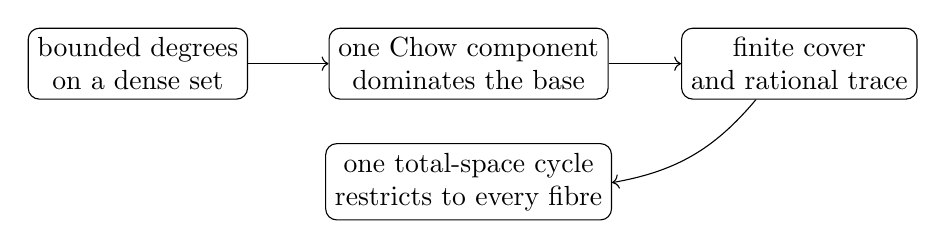
\begin{tikzpicture}[x=1cm,y=1cm]
\node[draw,rounded corners,align=center] (a) at (0,0)
 {bounded degrees\\on a dense set};
\node[draw,rounded corners,align=center] (b) at (4.2,0)
 {one Chow component\\dominates the base};
\node[draw,rounded corners,align=center] (c) at (8.4,0)
 {finite cover\\and rational trace};
\node[draw,rounded corners,align=center] (d) at (4.2,-1.5)
 {one total-space cycle\\restricts to every fibre};
\draw[->] (a)--(b);
\draw[->] (b)--(c);
\draw[->] (c) to[bend left=20] (d);
\end{tikzpicture}
\caption{Proper parameter spaces convert a uniform geometric
complexity bound into a global algebraic cycle. Density alone
does not provide the bound.}
\end{figure}

\begin{corollary}[Complexity on a curve]
\label{v7:new:cor:escape}
Suppose \(S\) is a curve and \(\Sigma(\gamma)\ne S\). Then
\(\Sigma_D(\gamma)\) is finite for every \(D\). Consequently, if
\(s_1,s_2,\ldots\) are distinct points of \(\Sigma(\gamma)\), the
smallest support-degree bound needed to span \(\gamma_{s_j}\)
tends to infinity.
On a curve algebraicity at an uncountable set of fibres suffices
for all the conditions of Theorem~\ref{v7:new:thm:global}.
\end{corollary}

\begin{proof}
Each \(\Sigma_D\) is a proper closed subset of a curve, hence finite.
Every fixed \(D\) therefore occurs at only finitely many terms of the
sequence. The union over \(D\) is countable unless it is all of \(S\).
\end{proof}

\section{A weaker test using one detected support}

The next criterion avoids requiring the target class itself to lie
in the span of the bounded-degree supports. Its constant-subsystem
hypothesis is essential to prevent cancellation under trace.

\begin{theorem}[Bounded-degree detection]
\label{v7:new:thm:detection}
Assume that a relative rational algebraic correspondence gives a flat
projector \(\Pi\) on \(R^{2p}f_*\Q\). Let \(W\) be a constant rational
sub-local system of \(\operatorname{im}\Pi\). Assume that at every
very general fibre,
\[
 \Pi\bigl(\Hdg^p(\mathcal Y_s)\bigr)\subseteq W_s.
\]
Suppose that for some \(D\), at a Zariski dense set of points \(s\)
there is an integral codimension-\(p\) subvariety \(V_s\), of degree
at most \(D\), with \(\Pi_s[V_s]\ne0\). Then there is a nonzero
global flat section \(w\) of \(W\), algebraic on every fibre and
represented by a relative total-space rational cycle.
\end{theorem}

\begin{proof}
For each degree at most \(D\), parameterize effective cycles by the
relative Chow variety. On each connected component, vanishing of
the projected cycle class is a flat, hence componentwise, condition.
The images of components on which it is nonzero are finitely many
closed subsets. The hypothesis makes their union dense, so one
irreducible such component \(T\) dominates \(S\).

Choose a point over a very general fibre. By the generic-image hypothesis its projected class
belongs to \(W\). Flatness makes membership in \(W\), and nonvanishing,
valid everywhere on \(T\). Since \(W\) is constant and \(T\) connected,
the projected class is a single fixed nonzero vector \(w\in W\).

Take a finite generic multisection and trace its cycle as in
Theorem~\ref{v7:new:thm:global}. After applying the algebraic projector,
every conjugate has class \(w\), so the trace has class
\([K':K]w\), not zero. Divide by the degree and close up.
The resulting total-space cycle represents \(w\) on every fibre.
\end{proof}

\begin{remark}
For a nonconstant local system, conjugate projected classes can sum
to zero. Nonvanishing at one point alone would not justify the trace
step. The generic-image hypothesis and the constancy of \(W\) are the additional
information used here.
\end{remark}

\subsection*{Application to the matched Mumford mixed class}

In the full-v7 notation, let
\[
 \mathcal Y=\mathcal X\times_S\mathcal X\times_S\mathcal Z,\qquad
 \Pi=\pi_1^{\mathcal X}\otimes\pi_1^{\mathcal X}
                         \otimes\pi_{T_Z}.
\]
Here \(\pi_1\) is the degree-one projector and \(\pi_{T_Z}\) is the
algebraic degree-two projector onto the rank-nine adjoint summand.
Their relative versions are available after the common finite level
cover used to define the two abelian schemes:
\begin{itemize}
\item interpolation in multiplication by two supplies relative
degree projectors;
\item a fixed element of the right norm-one torus supplies the
relative neutral-weight projector;
\item the Tate classes to be subtracted are generated by fixed
right-\(F\) pullbacks of a relative polarization, and their constant
intersection matrix supplies the relative divisor projector.
\end{itemize}
For the last item, squares span \(F\) over \(\Q\), since
\(u=((u+1)^2-(u-1)^2)/4\). Thus finitely many right-\(F\)
endomorphisms suffice. Their divisor classes and rational dual
intersection matrix are algebraic over the same level cover.

At a full-group fibre, the Hodge classes in the image of \(\Pi\)
are exactly
\[
 W=F\xi.
\]
Indeed \(T_X\) has multiplicity one in \(H^1(X)\otimes H^1(X)\),
\(T_Z\) is its irreducible rank-nine partner, and the commuting
field is \(F\). Both summands vary through the same left group,
so this is a constant rank-three rational subsystem.

Consequently, if one can find a fixed \(D\) and infinitely many
distinct fibres carrying one degree-\(\le D\) codimension-two
support with nonzero mixed projection, Theorem~\ref{v7:new:thm:detection}
produces a global class \(e\xi\), with \(0\ne e\in F\).
The already constructed algebraic \(F\)-action on \(T_Z\) applies
\(e^{-1}\) and produces \(\xi\) itself. The full-group transfer
theorem then gives every Hodge class on every power of \(X\) at
such a fibre.

The matched CM construction proves that some support with nonzero
mixed projection exists at each point of its isogeny orbit.
It does not bound the degrees of these supports uniformly.
Theorem~\ref{v7:new:thm:detection} weakens the required geometric input,
but does not supply it. It does not prove the universal statements
F2 or F3'.


% Proposed insertion. Not a proof of universal (F3').
% Uses the notation and bibliography of full-paper/main.tex.
\section{Transfer Defects and Primitive Hodge Classes}
\label{v7:ssec:exact-transfer-defects}

We make the effect of the proposed geometric operations explicit.
These are consequences of the classical correspondence formulas,
not a claim that the remaining defect vanishes. For either
\(\mathcal U^p(X)=\Alg^p(X)\) or
\(\mathcal U^p(X)=\Ab^p(X)\), put
\[
 D_{\mathcal U}^p(X)=\Hdg^p(X)/\mathcal U^p(X).
\]
All three spaces are zero outside \(0\le p\le\dim X\).
Algebraic correspondences act on these quotients: they preserve
Hodge classes, send cycle classes to cycle classes, and preserve
\(\Ab\) by composition with its defining correspondences.
Moreover \(\Alg^p(X)\subseteq\Ab^p(X)\), since a cycle can be
used as a correspondence from a point.

\begin{proposition}[Projective bundles and blow-ups]
\label{v7:prop:exact-defect-decomposition}
Let \(\mathscr E\) have rank \(r+1\) on a smooth projective
variety \(X\). Let \(b:W\to X\) be the blow-up of a smooth
centre \(Z\) of codimension \(c\ge2\). For either choice of
\(\mathcal U\), there are isomorphisms
\begin{align*}
 D_{\mathcal U}^p(\PP_X(\mathscr E))
   &\cong\bigoplus_{j=0}^{r}D_{\mathcal U}^{p-j}(X),\\
 D_{\mathcal U}^p(W)
   &\cong D_{\mathcal U}^p(X)
          \oplus\bigoplus_{j=1}^{c-1}
                     D_{\mathcal U}^{p-j}(Z).
\end{align*}
The maps and their inverses are induced by algebraic
correspondences. In particular the formulas hold for the
\Fiii{} defect, as well as for the algebraicity defect.
\end{proposition}

\begin{proof}
The classical projective-bundle and blow-up decompositions are
realized by algebraic correspondences \cite[\S\S7,9]{Man68}.
We specify inverses in order to check what happens to \(\Ab\).
Write \(\pi:P=\PP_X(\mathscr E)\to X\),
\(\xi=c_1(\mathcal O_P(1))\), and
\[
 I_j(\alpha)=\xi^j\pi^*\alpha,
 \qquad u_\ell=\pi_*\xi^{r+\ell}\quad(\ell\ge0).
\]
The classes \(u_\ell\) are algebraic, and \(u_0=1\).
If \(x=\sum_{j=0}^r I_j(\alpha_j)\), its coefficients are
recovered downwards by
\[
 \alpha_r=\pi_*x,\qquad
 \alpha_j=\pi_*(\xi^{r-j}x)
             -\sum_{k=j+1}^r u_{k-j}\alpha_k
       \quad(j=r-1,\ldots,0).
\]
Indeed \(\pi_*(\xi^{r-j}I_k(\alpha_k))\) is zero for
\(k<j\), is \(\alpha_j\) for \(k=j\), and is
\(u_{k-j}\alpha_k\) for \(k>j\). Every map in this recursion
is an algebraic correspondence. Thus the decomposition and its
inverse preserve \(\Hdg\), \(\Alg\), and \(\Ab\), with the
indicated codimension shifts. Passing to their quotients gives
the first formula.

For the blow-up, write \(i:Z\hookrightarrow X\),
\(j:E\hookrightarrow W\), \(q:E\to Z\), and
\(h=c_1(\mathcal O_E(1))\). The cohomology decomposition is
\[
 x=b^*\alpha+
       \sum_{k=1}^{c-1}j_*(h^{k-1}q^*\beta_k).
\]
Pushforward by \(b\) recovers \(\alpha\):
\(b_*b^*=\mathrm{id}\), whereas
\(b_*j_*(h^{k-1}q^*\beta_k)=i_*q_*(h^{k-1}q^*\beta_k)=0\)
because \(k-1<c-1\). Set \(x_0=x-b^*b_*x\). Since the
normal bundle of \(E\) in \(W\) is \(\mathcal O_E(-1)\),
self-intersection gives
\[
 j^*x_0=-\sum_{k=1}^{c-1}h^kq^*\beta_k.
\]
Apply the already explicit projective-bundle inverse for
\(q:E\to Z\) to recover every \(-\beta_k\).
Consequently all coefficient extractions are algebraic
correspondences. They preserve the two choices of
\(\mathcal U\), and the second quotient formula follows.
\end{proof}

\begin{proposition}[A trace splitting and finite quotients]
\label{v7:prop:trace-defect-splitting}
Let \(f:Y\to X\) be a surjective generically finite morphism
of smooth projective varieties, of degree \(d\). The algebraic
correspondence
\[
 e=\frac1d f^*f_*
\]
is an idempotent on \(H^*(Y,\QQ)\), and on each defect quotient
it gives a direct sum
\[
 D_{\mathcal U}^p(Y)
    =f^*D_{\mathcal U}^p(X)
        \oplus(1-e)D_{\mathcal U}^p(Y).
\]
If a finite group \(G\) acts on \(Y\) and \(X=Y/G\) is
smooth, then
\[
 D_{\mathcal U}^p(X)
      \cong D_{\mathcal U}^p(Y)^G.
\]
\end{proposition}

\begin{proof}
The projection formula and the degree identity give
\(f_*f^*=d\,\mathrm{id}\). Pullback and pushforward preserve
the numerator and denominator of the defect quotient. Thus
\(f^*\) is injective on that quotient, \(e^2=e\), and its image
is exactly \(f^*D_{\mathcal U}^p(X)\). Every idempotent splits
a vector space as its image and the image of its complement.

In the quotient case one can replace \(G\) by its effective
image, without changing its invariants. The generic fibre of
\(f\) is then a free orbit of cardinality \(|G|\). As cycles
of dimension \(\dim Y\), the fibre-product correspondence is
the sum of the graphs of the elements of \(G\); the ramification
loci have smaller dimension and introduce no additional
component of that dimension. Hence
\[
 f^*f_* = \sum_{g\in G}g^*,\qquad
 e=\frac1{|G|}\sum_{g\in G}g^*.
\]
This is the averaging projector, whose image on every rational
\(G\)-representation is its invariant subspace. Apply the
first assertion to the defect quotient.
\end{proof}

\begin{corollary}[The low-codimension boundary]
\label{v7:cor:stable-defect}
For either \(\mathcal U\), the quotient
\(D_{\mathcal U}^2(X)\) is a stable birational invariant of
smooth projective varieties. If \(\dim X=d\), the quotient
\(D_{\mathcal U}^{d-2}(X)\) is likewise invariant under
birational maps, and under stabilization it satisfies
\[
 D_{\mathcal U}^{d+r-2}(X\times\PP^r)
     \cong D_{\mathcal U}^{d-2}(X).
\]
In particular a smooth projective stably rational variety of
dimension at most five has zero defect in every degree, for
both choices of \(\mathcal U\).
\end{corollary}

\begin{proof}
The defects in codimensions \(0,1,m-1,m\) on a smooth
projective \(m\)-fold are zero, by Lefschetz \((1,1)\),
hard Lefschetz, and the unit and point classes. They also vanish
outside that range. For a blow-up of a \(d\)-fold, the new
terms in codimension two are \(D_{\mathcal U}^1(Z)\),
\(D_{\mathcal U}^0(Z)\), and zero terms. In codimension
\(d-2\), their indices satisfy
\[
 d-2-j\ge d-c-1=\dim Z-1
 \quad(1\le j\le c-1),
\]
so these terms vanish as well. Weak factorization
\cite{AKMW02} gives the birational assertions. The
projective-bundle formula gives the two stabilization
assertions: for codimension two all lower-index terms vanish;
for codimension \(d+r-2\), the only possibly nonzero summand
has index \(d-2\). In dimensions at most five these and the
already algebraic boundary degrees exhaust every codimension.
Stable rationality then compares them to projective space.
\end{proof}

\begin{proposition}[An explicit primitive projector on Hodge classes]
\label{v7:prop:primitive-hodge-projector}
Let \(X\) be a smooth projective \(d\)-fold, \(d\ge4\), and
let \(h\) be an ample divisor class. Let \(D_1,\ldots,D_\rho\)
be divisor classes forming a rational basis of \(\Hdg^1(X)\).
The matrix
\[
 Q_{ij}=\int_X D_iD_jh^{d-2}
\]
is invertible. The algebraic correspondence
\[
 \Pi_{\mathrm{np}}=
  \sum_{i,j=1}^{\rho}(Q^{-1})_{ij}
          (D_jh^{d-3})\times(hD_i)
       \in\operatorname{CH}^{d}(X\times X)_{\QQ}
\]
is an idempotent on cohomology. On \(\Hdg^2(X)\) its image is
\(h\Hdg^1(X)\), and its complement is the primitive part
\[
 P_h\Hdg^2(X)=
  \ker\bigl(h^{d-3}:\Hdg^2(X)\to\Hdg^{d-1}(X)\bigr).
\]
For either choice of \(\mathcal U\), it induces an isomorphism
\[
 D_{\mathcal U}^2(X)
    \cong
 \frac{P_h\Hdg^2(X)}
      {P_h\Hdg^2(X)\cap\mathcal U^2(X)}.
\]
Thus \Fiii{} in degree four is equivalent to the same
generation statement for primitive classes, with every
correspondence postcomposed by
\(\Delta_X-\Pi_{\mathrm{np}}\).
\end{proposition}

\begin{proof}
The Hodge index theorem makes \(Q\) nondegenerate: the line
spanned by \(h\) is positive, and its orthogonal complement
in \(\Hdg^1(X)_{\RR}\) is negative definite for this form.
In particular its inverse has rational coefficients. The
displayed correspondence acts on \(H^4(X,\QQ)\) by
\[
 \alpha\longmapsto
   h\sum_{i,j}D_i(Q^{-1})_{ij}
           \int_X\alpha D_jh^{d-3}.
\]
It is zero on other cohomological degrees, by degree. On each
\(hD_k\) this formula is the identity; its entire image is
in their span. It is therefore an idempotent on cohomology.

For \(\alpha\in\Hdg^2(X)\), hard Lefschetz gives a unique
\(\beta\in\Hdg^1(X)\) such that
\[
 h^{d-2}\beta=h^{d-3}\alpha.
\]
Write \(\beta=\sum_i b_iD_i\). Pairing this equality with
each \(D_j\) gives \(\sum_iQ_{ji}b_i
=\int_X\alpha D_jh^{d-3}\). Hence the formula above is
exactly \(h\beta\), and \(\alpha-\Pi_{\mathrm{np}*}\alpha\)
is primitive. Conversely a primitive Hodge class has every
one of these pairings zero and is annihilated by
\(\Pi_{\mathrm{np}*}\). This proves the decomposition on
Hodge classes.

Its nonprimitive summand is algebraic, since every \(D_i\)
is a divisor class. It is therefore contained in either
\(\mathcal U^2(X)\). Subtracting this summand from a
representative proves the quotient isomorphism. The
complementary projector is algebraic and preserves \(\Ab\),
so applying it to every term of a transfer expression yields
the last assertion.
\end{proof}

The last projector concerns rational Hodge classes in degree
four. It is not asserted to be the full primitive projector on
\(H^4(X,\QQ)\); the non-Hodge part of \(hH^2(X,\QQ)\) is
not removed by its divisor formula. No algebraicity of a
general inverse Lefschetz operator is being assumed. The
construction removes only the already algebraic summand.
It provides no representative, or correspondence from an
abelian variety, for the remaining primitive quotient.


\section{Where the earlier attempt fails}\label{sec:earlier}

The preprint \cite{BB26} of the two authors claimed the conjecture in full. We record here each point at which it fails, so that the present paper can be read as its replacement and not as a continuation. Numbers refer to that preprint.

\paragraph{The secant cycle (Definition 3, Lemma 4).} For an abelian $2n$-fold $A$ of Weil type the preprint takes $\Sigma=\mathrm{Sec}^{n}(A^{\vee})$, the closure of the union of the $(n-1)$-planes spanned by $n$ points of $A^{\vee}$ in a projective embedding, and the cycle $Z_{\Sigma}=\Sigma\cap A^{\vee}$, asserted to have codimension $n$. Every point of $A^{\vee}$ lies on such a plane, so $A^{\vee}\subseteq\Sigma$ and $Z_{\Sigma}=A^{\vee}$: the intersection is not proper. The sheaf $\mathcal{O}_{\Sigma}|_{A^{\vee}}$ is $\mathcal{O}_{A^{\vee}}$, whose Fourier--Mukai transform is the skyscraper sheaf at the origin shifted by $-2n$, with Chern character the class of a point. So $\ch_{k}=0$ for $1\le k<2n$, contrary to Lemma~4, and Proposition~2 has nothing to identify with a Weil class.

\paragraph{The polarisation (Definition 3).} The polarisation is taken principal, so $\chi(L)=1$ and the embedding is into $\PP^{0}$; the dimension count needs $\chi(L)=2n^{2}+2n$. A principal polarisation is never very ample.

\paragraph{The dimension of the Weil space (Proposition 1).} $\det_{K}H^{1}(A)$ is a two-dimensional $\QQ$-space of Hodge classes \cite{Weil77}, so at a very general point $\Hdg^{n}(A)=\QQ\eta^{n}\oplus W(A)$ has dimension three, not two.

\begin{figure*}[t]
\centering
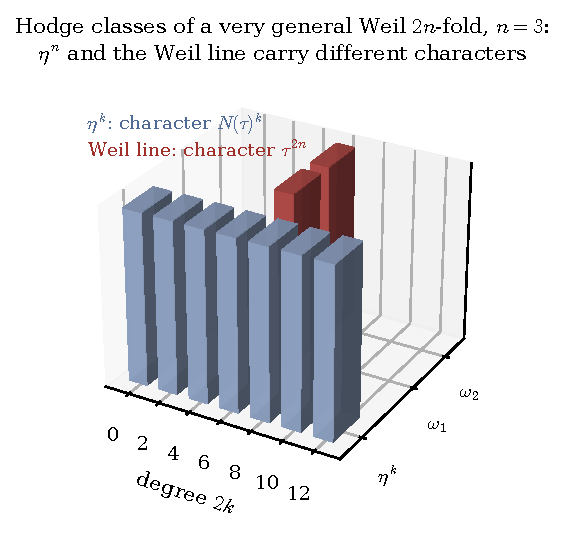
\includegraphics[width=0.92\textwidth]{figures/fig_eigen}
\caption{The Hodge classes of a very general abelian sixfold of Weil type and the characters of $K^{\times}$ on them: $\eta^{k}$ carries $N(\tau)^{k}$, the Weil plane carries $\tau^{2n}$. An eigenclass for $N^{n}$ in degree $2n$ is a multiple of $\eta^{n}$.}
\label{fig:eigen}
\end{figure*}

\paragraph{The eigencharacter (Lemmas 1, 2, Proposition 2, Theorem 4).} Equation~(1) of the preprint gives $\tau^{*}\eta=N(\tau)\eta$ for $\tau\in K^{\times}$, so $\eta^{n}$ has character $N(\tau)^{n}$, while Proposition~2 asserts character $1$. The group $K^{\times}$ acts on $W(A)=\bigwedge^{2n}_{K}H^{1}(A)$ by $\tau\mapsto\tau^{2n}$, which differs from $N(\tau)^{n}=(\tau\bar\tau)^{n}$ unless $(\tau/\bar\tau)^{n}=1$; so the Weil classes are not in the $N^{n}$-eigenspace, and an $N^{n}$-eigenclass of degree $2n$ is a multiple of $\eta^{n}$ (Fig.~\ref{fig:eigen}). The scaling of the secant sheaf by $d^{n}$ under an isogeny of degree $d$ (Lemma~1) is asserted without proof.

\paragraph{Step 4 of Theorem 4.} The points of a Shimura variety with smaller Mumford--Tate group are the points of proper special subvarieties, most of which are not of CM type; and Pohlmann's theorem \cite{Poh68} covers the CM types whose Hodge ring is generated by divisors, not all CM abelian varieties.

\paragraph{The reduction to Weil classes (Theorem 3, Section 5).} Moonen and Zarhin describe every Hodge class as a polynomial in divisor classes and Weil classes of isogeny factors in dimension at most five \cite{MZ99}, and the description is not known beyond; simple CM abelian varieties can carry Weil classes \cite{Weil77,Shi79b}; and not every factor of type IV is of Weil type.

\paragraph{Theorem 12.} The Kuga--Satake construction exists for Hodge structures of K3 type, with $h^{2,0}=1$ \cite{KS67,Del72}; Theorem~12 applies it to arbitrary primitive classes. Its algebraicity, credited there to Deligne, is open: Deligne proved that the correspondence is absolutely Hodge \cite{Del82}, and its algebraicity is known only in special families \cite{vG00,Var23}. Since the case split of Section~1.4 rests on this step for the classes of coniveau zero, it is incomplete.

None of these points is repaired here. The present paper does not use secant cycles, the eigencharacter argument or the Kuga--Satake construction outside K3 type, and it claims no case of the conjecture that is not proved in Sections~\ref{sec:reduction} to \ref{sec:v7-bypass}.

\begingroup
\small\setlength{\tabcolsep}{3pt}\setlength{\LTleft}{0pt}\setlength{\LTright}{0pt}
\begin{longtable}{@{}>{\raggedright\arraybackslash}p{.42\textwidth}>{\raggedright\arraybackslash}p{.18\textwidth}>{\raggedright\arraybackslash}p{.15\textwidth}>{\raggedright\arraybackslash}p{.18\textwidth}@{}}
\caption{Status of the retained and new statements. Conditional transfers do not assert their missing input.}\label{tab:status}\\
\toprule
statement & where & status & what it needs \\
\midrule
$\HC\Leftrightarrow\Fii{}\wedge\Fiii{}$ & Thm.~\ref{thm:intro-reduction} & proved & -- \\
\Fiii{} for fourfolds with zero-cycles on a threefold & Prop.~\ref{prop:fourfold} & proved from \cite{BS83} & -- \\
\Fii{} $\Leftrightarrow$ $\AB$ & Thm.~\ref{thm:f2isab} & proved & -- \\
six minimal sufficient sets & Prop.~\ref{prop:minimal} & proved, checked in Lean & -- \\
dichotomy of the algebraic locus & Lem.~\ref{lem:dichotomy} & proved & -- \\
\Fii{} as propagation from CM points & Thm.~\ref{thm:propagation} & proved & -- \\
Weil loci dense with CM base point & Prop.~\ref{prop:weil-dense} & proved in \cite{BMB26} & -- \\
chains make $e$ with $e^{2}\in\QQ$ algebraic & Thm.~\ref{thm:chain} & proved & a chain of the right multiplier \\
symplectic chains reach exactly $\sqrt2,\sqrt3,\sqrt6$ & Prop.~\ref{prop:sqrt10} & proved & -- \\
$\sqrt6$ algebraic on two-dimensional families & Thm.~\ref{thm:sqrt6} & proved & -- \\
$\sqrt{-5}$, $\sqrt{-7}$ algebraic on one-dimensional families & Thm.~\ref{thm:fricke} & proved & -- \\
$\HC$ on all powers and Hilbert schemes of the Fricke surfaces & Thm.~\ref{thm:fricke} & proved & -- \\
similarities act by multipliers $d_{1}d_{2}$ & Prop.~\ref{prop:structure} & proved & -- \\
finite-group correspondences give abelian $E$ & Prop.~\ref{prop:hecke} & proved & -- \\
$\HC$ for $X\times X$, $X$ in the dihedral families & Cor.~\ref{cor:dihedral} & proved & -- \\
\Fiii{} for $S_{\lambda}$, $F=\QQ(\zeta_{7})^{+}$ or $\QQ(\zeta_{9})^{+}$, $D=D_{\infty}$ & Thm.~\ref{thm:zeta9} & proved & -- \\
where the dihedral mechanism stops & Prop.~\ref{prop:cubicstop} & proved & -- \\
\Fiii{} for $S_{\lambda}$, other cubic $F$ or other $D$ & Sect.~\ref{ssec:f3stop} & open & a non-similarity correspondence \\
Hodge classes on all powers of $S$: $E$ and $\bigwedge^{m}_{E}T$ & Prop.~\ref{prop:powers} & proved from \cite{Var25} & -- \\
K3 surfaces of Kummer type over $\QQ$: \Fiii{} and $\HC$ on all powers & Prop.~\ref{prop:kummerq} & proved & -- \\
Fricke Kuga--Satake fourfold: $B\sim E_{K}\times B_{3}$ & Prop.~\ref{prop:frickeks} & proved & -- \\
$\bigwedge^{m}_{E}T$ for the other surfaces of Sect.~\ref{sec:f3prime} & Rem.~\ref{rem:detfrontier} & open & a cycle on $S^{m}$ \\
\Fiii{} in general & -- & open & -- \\
product object of polarised shape & Thm.~\ref{thm:product} & proved & -- \\
direct sums never semiregular & Prop.~\ref{prop:directsum} & proved & -- \\
annihilator of the secant pieces is the product locus & Thm.~\ref{thm:annihilator} & proved & -- \\
secant and line-bundle pieces orthogonal & Prop.~\ref{prop:noorth} & false for every realisation & -- \\
(P2$'$) at a product point & Sect.~\ref{ssec:f2stop1} & open & $\Ext^{*}$ of secant sheaves \\
the Ext groups at the CM point $E_{0}^{6}$ & Lem.~\ref{lem:cmext} & proved & -- \\
no two-step cancellation of diagonal classes & Prop.~\ref{prop:twostep} & proved & -- \\
three line bundles at $E_{0}^{6}$ & Prop.~\ref{prop:separated} & proved, fail & -- \\
isolated Ext blocks at $E_{0}^{6}$ & Prop.~\ref{prop:e06count} & proved, fail & -- \\
a threefold piece outside every closed chain & Prop.~\ref{prop:chainfree} & proved, fail & -- \\
further pieces within one shift of the thirty-two & Cor.~\ref{cor:chainfree} & proved, fail & -- \\
at most five line bundles, any twists, every polarisation & Thm.~\ref{thm:fivebundles} & proved, fail & -- \\
six or seven line bundles; eight outside thirty-one cases & Rem.~\ref{rem:sevenbundles} & enumeration, fail & -- \\
the rest of the support cuts a threefold in an ample divisor & Thm.~\ref{thm:locality} & proved & -- \\
two threefolds meeting along a surface carry nothing & Thm.~\ref{thm:pair} & proved & -- \\
objects on the thirty-two threefolds of one family & Cor.~\ref{cor:threefolds} & proved, fail & -- \\
objects on the sixty-four threefolds of both families & Thm.~\ref{thm:sixtyfour} & proved, fail & -- \\
a smooth complete intersection cannot carry the rest & Prop.~\ref{prop:ci} & proved, fail & -- \\
an ample divisor in the support empties the localised obstruction & Prop.~\ref{prop:stops} & proved & -- \\
(P2$'$) at $E_{0}^{6}$: eight or more line bundles, with or without threefolds & Sect.~\ref{ssec:supports} & open & the chain products \\
$E_{0}^{8}$: shifts in seven consecutive integers & Cor.~\ref{cor:efourseven} & 18 of 28 proved & -- \\
an \'etale Prym map of triple covers at genus four & Prop.~\ref{prop:genusfour} & proved & -- \\
sextic CM fields: the count excludes nothing & Rem.~\ref{rem:sexticfields} & enumeration & -- \\
sixfold link $\Rightarrow$ exceptional classes & Thm.~\ref{thm:link} & proved & -- \\
algebraicity of the generic link $\xi$ & Sect.~\ref{ssec:f2stop2} & open & a cycle on $X\times X\times Z_{K}$ \\
dominant maps, blow-ups, derived equivalences preserve the defect & Prop.~\ref{prop:surgery} & proved & -- \\
residues of complete intersections & Prop.~\ref{prop:residues} & proved & rational residues \\
$\HC$ for $\alpha$ as a vanishing mass gap & Prop.~\ref{prop:mass} & proved & -- \\
exceptional classes of $X\times X$ & -- & open & -- \\
\Fii{} in general & -- & open & -- \\
the Hodge conjecture & -- & open & \Fii{} and \Fiii{} \\

matched CM mixed link & Thm.~\ref{v7:thm:seed} & proved & matched torus choice \\
adjoint projector and $F$-action on $Z$ & Prop.~\ref{v7:prop:proj} & proved & -- \\
all powers of the auxiliary sixfold & Prop.~\ref{v7:prop:sixfold} & proved & full-group fibre \\
one exceptional class implies all powers & Prop.~\ref{v7:prop:square} & conditional transfer & one algebraic exceptional class \\
CM weight-one maps fail at first order & Prop.~\ref{v7:prop:firstorder} & proved & -- \\
pure Chern representative at the seed & Prop.~\ref{v7:prop:adams} & proved & not a deformation theorem \\
Chern character alone does not deform bundles & Thm.~\ref{v7:k3-obstructed-bundle} & proved counterexample & -- \\

\bottomrule
\end{longtable}
\endgroup

\section{What is proved and what is open}\label{sec:status}


Table~\ref{tab:status} lists the statements. Three remarks on what the table says.

The two universal statements have distinct remaining requirements. For the named Shimura and Weil families one has a dense algebraic locus, and the question is whether a component dominates the base. For arbitrary varieties, \Fiii{} additionally requires algebraic correspondences that have not been constructed. Density in these special families does not establish that universal requirement. For \Fii{} the dense set is supplied by explicit cycles at CM points and the first instance is a single class on an abelian fourteenfold or a single Ext group on an eightfold; for \Fiii{} the dense set is supplied by the K3 surfaces with complex multiplication and by the chains of Section~\ref{sec:f3prime}, and the first instance is a cubic real multiplication on one K3 surface of Picard number $13$, which Theorem~\ref{thm:zeta9} supplies for the fields $\QQ(\zeta_{7})^{+}$ and $\QQ(\zeta_{9})^{+}$ with the algebra ramified at two real places, and which stays open for every other pair of a cubic field and an algebra.

Each construction of this paper ends at a question with a definite answer. Whether some convolution of the pieces of Theorem~\ref{thm:product} has $\dim\Ext^{2}=57$ is a finite computation in the Ext algebra of two sheaves on a fourfold; at the point $E_{0}^{6}$ of complex multiplication every group entering it is written down in Lemma~\ref{lem:cmext}, Proposition~\ref{prop:separated} answers it in the negative for every convolution with three powers of $L$, Proposition~\ref{prop:e06count} answers it in the negative for two threefolds at one shift and for every placement of the thirty-five pieces, Proposition~\ref{prop:chainfree} with Corollary~\ref{cor:chainfree} for every further piece of positive twist within one shift of the thirty-two, Theorem~\ref{thm:fivebundles} for at most five line bundles at any twists and every polarisation, the enumeration of Remark~\ref{rem:sevenbundles} for six and seven and for eight outside thirty-one arrangements, Corollary~\ref{cor:threefolds} and Theorem~\ref{thm:sixtyfour} for every convolution of threefold pieces, of one family or of both, at any twists and shifts, and for the configurations left, eight or more line bundles with or without threefolds, it is the rank of the products along the chains of Proposition~\ref{prop:twostep} and along the cycles through the line bundles, the support of the object being constrained by Theorem~\ref{thm:locality} and Propositions~\ref{prop:rest} and \ref{prop:ci}. Whether the link $\xi$ is algebraic is a question about one Hodge class on one abelian variety, equivalent by Theorem~\ref{thm:link}(v) to the exceptional classes together with one more cycle. Whether a correspondence acting on $T(S_{\lambda})$ otherwise than by a similarity exists is a question about one K3 surface; for $F=\QQ(\zeta_{7})^{+}$ or $\QQ(\zeta_{9})^{+}$ and $D=D_{\infty}$ Theorem~\ref{thm:zeta9} answers it, and for every other pair $(F,D)$ it is open, with Proposition~\ref{prop:cubicstop} marking the three places where the present mechanism fails. A negative answer to the first closes that route, as the analogous question on $E_{0}^{6}$ closed; a positive answer to any of them proves the corresponding statement at its first instance.

\subsection{Specialisation, degeneration and blow-ups}\label{ssec:bypass}

Three devices are often proposed for passing from the members where a class is known to be algebraic to the others, and we record exactly what each one proves.

\begin{proposition}\label{prop:bypass}
Let $\pi:\mathcal{X}\to B$ be a smooth projective family over an irreducible base and $\xi$ a flat Hodge class on its fibres.
\begin{enumerate}[label=\textup{(\roman*)},leftmargin=2.4em,itemsep=2pt]
\item If $\xi_{t}$ is algebraic at the generic point of a curve $C\subseteq B$ then it is algebraic at every point of $C$. The converse implication, from one point of $C$ to its generic point, holds when $\xi_{t_{0}}$ is the Chern character of a perfect complex whose semiregularity map is injective, and in no greater generality is it known.
\item Let $\tilde X$ be the blow-up of a smooth projective variety $X$ along a smooth closed subvariety $Z$ of codimension $c$. Then $\Hdg^{k}(\tilde X)/\Alg^{k}(\tilde X)\cong\Hdg^{k}(X)/\Alg^{k}(X)\oplus\bigoplus_{i=1}^{c-1}\Hdg^{k-i}(Z)/\Alg^{k-i}(Z)$. In particular the Hodge conjecture for $\tilde X$ is equivalent to the Hodge conjecture for $X$ and for $Z$, and a blow-up never reduces the defect of a variety.
\item For the Weil classes of $\cD_{n,n}$ and the exceptional class of a Mumford fourfold, every degeneration to a fibre with a semistable model on which the limit class is algebraic has its lift to the generic fibre as its missing step, and for the Mumford fourfold no degeneration keeping the class of Hodge type exists, since the Hodge locus of the class is a compact Shimura curve.
\end{enumerate}
\end{proposition}

\begin{proof}
(i) Specialisation of cycles along a curve \cite[Ch.~20]{Ful98} sends an algebraic cycle on the generic fibre to one on each special fibre with the same flat cohomology class; this is the direction used by Schoen's degeneration and by Proposition~\ref{prop:weil-dense}. In the other direction the algebraic locus is a countable union of closed sets by Lemma~\ref{lem:dichotomy}, and a point in one stratum says nothing about the stratum being the whole base; the one proved lift is the semiregularity theorem of Bloch, Buchweitz and Flenner \cite{Blo72,BF03}, which is the content of Theorem~\ref{thm:criterion}. (ii) Manin's decomposition of the motive of a blow-up \cite{Man68}, $h(\tilde X)=h(X)\oplus\bigoplus_{i=1}^{c-1}h(Z)(-i)$, is realised by the algebraic correspondences $\pi^{*}$ and $j_{*}\circ p^{*}\circ(\text{powers of the relative hyperplane class})$, which are compatible with Hodge classes and with algebraic classes; so both the Hodge classes and the algebraic classes of $\tilde X$ decompose accordingly, and the quotients add. Since every summand is non-negative, the defect of $\tilde X$ is at least that of $X$, and a blow-down along a smooth centre $Z$ lowers the defect by exactly that of $Z$ in the shifted degrees. (iii) A flat class has a limit in the limit mixed Hodge structure of a semistable fibre, and on a totally degenerate fibre the graded pieces are combinatorial and every class is algebraic on the components; the return to the generic fibre is the lift of (i), with the same unproved step. For a Mumford fourfold the Hodge locus of the exceptional class is the compact Shimura curve of \cite[Thm.~21.7]{BMB26}, which has no boundary, so no fibre at which the class is still of Hodge type degenerates.
\end{proof}

\begin{figure*}[t]
\centering
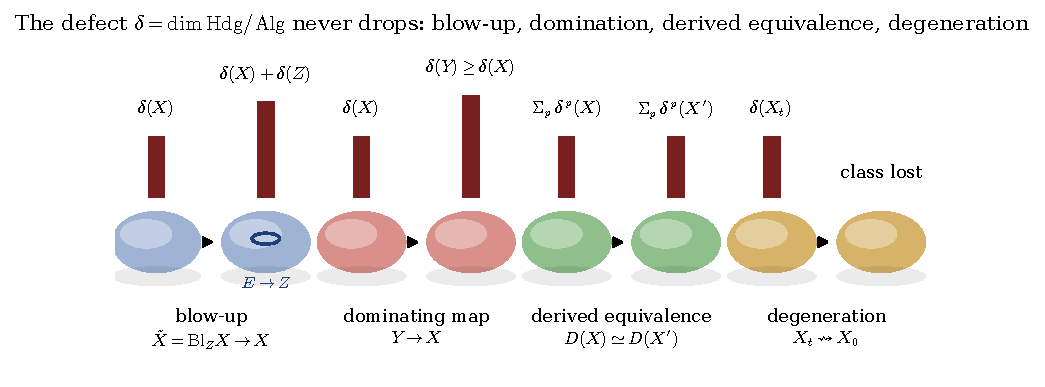
\includegraphics[width=0.92\textwidth]{figures/fig_surgery}
\caption{Where the defect goes under surgery. A blow-up along $Z$ carries the Hodge classes of $X$ to $\tilde X$ and adds those of $Z$, so the quotient $\Hdg/\Alg$ grows by the defect of the centre; a dominating map $Y\to X$ carries the defect of $X$ into $Y$; a Fourier--Mukai equivalence permutes degrees and preserves the total defect; a degeneration to $X_{0}$ loses the class only in the special fibre, from which no cycle lifts.}
\label{fig:surgery}
\end{figure*}

\subsection{Dominating maps, birational models and derived equivalences}\label{ssec:surgery}

Write $\delta^{p}(X)=\dim\Hdg^{p}(X)-\dim\Alg^{p}(X)$ for the defect of the conjecture in degree $2p$, $\delta_{\mathrm{ab}}^{p}(X)=\dim\Hdg^{p}(X)-\dim\Ab^{p}(X)$ for the defect of \Fiii{}, and $\delta(X)=\sum_{p}\delta^{p}(X)$. The conjecture for $X$ is $\delta(X)=0$. The following proposition records how the surgeries of birational geometry move these numbers; Figure~\ref{fig:surgery} draws it.

\begin{proposition}[Defects under surgery]\label{prop:surgery}
Let $X$, $Y$ be smooth complex projective varieties.
\begin{enumerate}[label=\textup{(\roman*)},leftmargin=2.4em,itemsep=2pt]
\item If $f\colon Y\to X$ is surjective and generically finite, then $\delta^{p}(Y)\ge\delta^{p}(X)$ and $\delta^{p}_{\mathrm{ab}}(Y)\ge\delta^{p}_{\mathrm{ab}}(X)$ for every $p$. In particular no blow-up along a singular centre, weighted blow-up, resolution of a modification or finite cover of $X$ has a smaller defect than $X$.
\item If $X$ and $Y$ are birational, then $\delta^{2}(X)=\delta^{2}(Y)$ and $\delta^{d-1}(X)=\delta^{d-1}(Y)$, $d=\dim X$; for $3\le p\le d-2$ the difference $\delta^{p}(X)-\delta^{p}(Y)$ is a signed sum of defects $\delta^{p-j}(Z)$, $j\ge1$, of smooth projective varieties $Z$ of dimension less than $d$.
\item If $\Gamma\in\mathrm{CH}^{*}(X\times Y)_{\QQ}$ induces an isomorphism from $H^{*}(X,\QQ)$ onto $H^{*}(Y,\QQ)$ whose inverse is induced by a cycle, for instance the kernel of an equivalence between the derived categories of $X$ and $Y$, then $\delta(X)=\delta(Y)$ and $\delta_{\mathrm{ab}}(X)=\delta_{\mathrm{ab}}(Y)$.
\item Let $\mathcal{X}\to\Delta$ be a projective family, smooth over the punctured disc, with a flat Hodge class $\xi$ on the smooth fibres that is algebraic on a crepant resolution $\hat X$ of the special fibre $X_{0}$, or on the components of a semistable model of $X_{0}$. Then $\xi$ is algebraic on $X_{t}$ for $t\ne0$ if and only if the specialisation $H^{2p}(X_{0})\to H^{2p}(X_{t})$ sends an algebraic class to an algebraic class, which is the statement (V) for the family; the monodromy plays no role, since it fixes $\xi$.
\end{enumerate}
\end{proposition}

\begin{proof}
(i) $f_{*}f^{*}$ is multiplication by the degree, so $f^{*}$ is an injective morphism of Hodge structures and $f^{*}\Hdg^{p}(X)\subseteq\Hdg^{p}(Y)$. If $f^{*}\alpha$ is algebraic then so is $\deg(f)\,\alpha=f_{*}f^{*}\alpha$; hence $\Alg^{p}(Y)\cap f^{*}\Hdg^{p}(X)=f^{*}\Alg^{p}(X)$ and $f^{*}$ embeds $\Hdg^{p}(X)/\Alg^{p}(X)$ into $\Hdg^{p}(Y)/\Alg^{p}(Y)$. For $\Ab$ the same argument applies because $f_{*}$ of a class $\Gamma_{*}\gamma$ reached from an abelian variety is $(\Gamma_{f}\circ\Gamma)_{*}\gamma$, reached from the same one. The coarse space of a weighted blow-up has quotient singularities and $f_{*}f^{*}=\mathrm{id}$ with rational coefficients, so the argument is unchanged there.

(ii) By weak factorisation \cite{AKMW02} a birational map between smooth projective varieties is a composite of blow-ups and blow-downs along smooth centres with smooth projective intermediate varieties, and Proposition~\ref{prop:bypass}(ii) gives the change of $\delta^{p}$ at each step as $\pm\sum_{j=1}^{c-1}\delta^{p-j}(Z)$. For $p=2$ the terms are $\delta^{1}(Z)$ and $\delta^{0}(Z)$, which vanish by the Lefschetz $(1,1)$ theorem; for $p=d-1$ they are $\delta^{d-1-j}(Z)$ with $\dim Z\le d-2$, hence $\delta^{q}(Z)$ with $q\ge\dim Z-1$ after $j\ge1$, and these vanish by hard Lefschetz and Lefschetz $(1,1)$ on $Z$.

(iii) By the projection formula $\Gamma_{*}$ sends $\bigoplus_{p}\Hdg^{p}(X)$ into $\bigoplus_{p}\Hdg^{p}(Y)$, since $[\Gamma]$ is a sum of classes of type $(i,i)$ and cup product and push-forward are morphisms of Hodge structures up to Tate twists; it sends algebraic classes to algebraic classes because $[\Gamma]\cup\mathrm{pr}_{X}^{*}[Z]$ is the class of a cycle and the push-forward of a cycle is a cycle; and it sends $\Ab$ to $\Ab$ by composing correspondences. The inverse does the same in the other direction, so the two total quotients are isomorphic. The kernel of a Fourier--Mukai equivalence and the kernel of its inverse are cycles by Mukai's and Orlov's description of the inverse functor \cite{Orl97}, which is the equivalence with kernel the dual of the original one shifted by the dimension.

(iv) $\xi$ is monodromy invariant, so by the local invariant cycle theorem it is the specialisation of a class in $H^{2p}(X_{0})$, which pulls back to $\hat X$ or to the components of the semistable model; the hypothesis says that the pulled back class is algebraic there, and push-forward keeps it algebraic on $X_{0}$. Cycles specialise from the generic fibre to the special fibre \cite[Ch.~20]{Ful98} and not the other way, so the remaining step is exactly the one in the statement. If the limit cycle on $X_{0}$ lifts to the family, its restriction to $X_{t}$ has class $\xi_{t}$; conversely if $\xi_{t}$ is algebraic the specialisation of a representing cycle is a cycle on $X_{0}$ with class the limit of $\xi$, and the specialisation map sends that class to $\xi_{t}$. The vanishing cycles, on which the monodromy acts, are orthogonal to the invariant part, and $\xi$ is invariant, so no condition on them enters.
\end{proof}

Items (i) to (iii) say that every surgery available in birational and derived geometry carries the defect of $X$ into its output as long as the open class survives there, and loses the class only in outputs of lower dimension, the centres, where it has become a defect of those varieties. Both open statements of this paper sit in degree four, \Fii{} for the Weil classes and the exceptional classes, \Fiii{} for the classes of $H^{4}(S\times S)$ on a K3 surface, and in degree four the defect is a strict birational invariant by (ii) and a derived invariant by (iii); so the open classes are present, and not known to be algebraic, on every birational model and every Fourier--Mukai partner of the varieties that carry them. Item (iv) is the reason that degenerations to products of elliptic curves, where every Hodge class is algebraic \cite{MZ99}, do not close \Fii{}: the class returns to the smooth fibre only through (V). Flows of K\"ahler metrics change no complex structure between their surgeries, and the surgeries themselves are the contractions and flips of the minimal model programme, covered by (i) and (ii); the surgery of Perelman has no counterpart for Hodge structures, since it cuts a manifold along spheres and a Hodge structure has no local pieces to cut.

The devices therefore relocate the two open statements without weakening them. The one true reduction in shape is Theorem~\ref{thm:propagation}: the whole of \Fii{} is equivalent to a lift from CM points along polarised abelian schemes, and the lift along each scheme is a question about one semiregular object at one point.

\subsection{Residues and mass-minimising currents}\label{ssec:analytic}

Two analytic descriptions of algebraic classes are exact, and we record what each reduces the conjecture to. The first is Griffiths' residue calculus on hypersurfaces \cite{Gri69}. For a smooth hypersurface $X=\{F=0\}\subset\PP^{n+1}$ of even dimension $n=2m$ and degree $d$, with Jacobian ring $R(F)$ and $\Omega=\sum_{i}(-1)^{i}x_{i}\,dx_{0}\wedge\dots\widehat{dx_{i}}\dots\wedge dx_{n+1}$, the residues of the forms $P\Omega/F^{q+1}$ identify $H^{n-q,q}_{\mathrm{prim}}(X)$ with $R(F)_{(q+1)d-n-2}$.

\begin{proposition}[Residues of complete intersections]\label{prop:residues}
Let $X=\{F=0\}$ be as above, and suppose that $F=\sum_{i=1}^{m+1}f_{i}g_{i}$ with $Z=\{f_{1}=\dots=f_{m+1}=0\}$ a complete intersection of codimension $m+1$ in $\PP^{n+1}$ whose ideal is generated by the $f_{i}$.
\begin{enumerate}[label=\textup{(\roman*)},leftmargin=2.4em,itemsep=2pt]
\item Let $\theta$ be the hyperplane class and $J_{H}$ the Jacobian determinant of $(f_{1},g_{1},\dots,f_{m+1},g_{m+1})$, a polynomial of degree $(m+1)(d-2)$. Then
\[
[Z]=\frac{\deg Z}{d}\,\theta^{m}-\frac{m!}{d}\,\operatorname{res}\Bigl(\frac{J_{H}\,\Omega}{F^{m+1}}\Bigr)^{m,m}
\]
\cite[Thm.~1.1]{VL22}.
\item Let $J(F)\subseteq R(F)_{(m+1)(d-2)}$ be the span of the classes of the determinants $J_{H}$ over all such decompositions of $F$. If the rational span of the residues of $J(F)$ and $\theta^{m}$ contains $\Hdg^{m}(X)$, the Hodge conjecture holds for $X$.
\end{enumerate}
\end{proposition}

\begin{proof}
(i) is the cited theorem; the degree of the determinant is $\sum_{i}(\deg f_{i}+\deg g_{i})-(n+2)=(m+1)d-2m-2$. (ii) By (i) every residue of an element of $J(F)$ is a rational combination of $\theta^{m}$ and of classes of complete intersections in $X$, so it is algebraic. The Hodge conjecture for a hypersurface holds outside the middle degree by the Lefschetz hyperplane theorem, and in the middle degree it is the statement that $\Hdg^{m}(X)$ consists of algebraic classes.
\end{proof}

The proposition replaces a cycle by a polynomial, and the open step becomes the statement that the polynomials of $J(F)$ have enough rational residues. Deciding whether a given element of $R(F)$ has a rational residue requires its periods, so the residue calculus moves the conjecture from cycles to transcendental numbers without closing it. On a Fermat hypersurface $\sum_{i}x_{i}^{d}=0$ the linear subspaces cut out by $x_{2i}=\zeta_{i}x_{2i+1}$, $\zeta_{i}^{d}=-1$, are of this form, since $x_{2i}^{d}+x_{2i+1}^{d}$ factors into linear forms; whether their residues and those of the other decompositions exhaust $\Hdg^{m}(X)$ is again a question about periods.

The second description uses currents and is the analogue for cycles of the flows of geometric analysis. Let $X$ be a smooth complex projective variety of dimension $N$, $h$ an ample class with K\"ahler form $\omega$, and $0<p<N$. For $\beta\in H_{2(N-p)}(X,\ZZ)$ let $M(\beta)$ be the infimum of the masses of the integral currents in $\beta$, put $\mathrm{vol}(\beta)=\int_{\beta}\omega^{N-p}/(N-p)!$, and call $g(\beta)=M(\beta)-\mathrm{vol}(\beta)$ the gap of $\beta$. We identify $H^{2p}(X,\ZZ)$ with $H_{2(N-p)}(X,\ZZ)$ by Poincar\'e duality.

\begin{proposition}[Mass-minimising currents]\label{prop:mass}
\leavevmode
\begin{enumerate}[label=\textup{(\roman*)},leftmargin=2.4em,itemsep=2pt]
\item Every class $\beta$ contains an integral current of mass $M(\beta)$, and $g(\beta)\ge0$, with equality if and only if $\beta$ is the class of an effective algebraic cycle with integer coefficients.
\item Let $\alpha\in H^{2p}(X,\ZZ)$. The image of $\alpha$ in $H^{2p}(X,\QQ)$ is algebraic if and only if $g(e\alpha+kh^{p})=0$ for some integers $e\ge1$ and $k\ge0$.
\item There are $X$ and $\alpha$ with $g(\alpha+kh^{p})>0$ for every $k\ge0$ although $g(e\alpha)=0$ for some $e\ge1$: for a very general hypersurface $X\subset\PP^{4}$ of degree $D$ divisible by $\ell^{3}$ for an integer $\ell>1$ prime to $6$, $p=2$, and the generator $\alpha$ of $H^{4}(X,\ZZ)$.
\end{enumerate}
\end{proposition}

\begin{proof}
(i) By the compactness theorem of Federer and Fleming \cite{FF60} the integral currents in $\beta$ of mass at most $M(\beta)+1$ form a compact set for the flat topology, and mass is lower semicontinuous, so the infimum is attained. For an integral current $T$ in $\beta$, Wirtinger's inequality, that $\omega^{N-p}/(N-p)!$ has comass one with equality exactly on the complex $(N-p)$-planes with their canonical orientation, gives $M(T)\ge T\bigl(\omega^{N-p}/(N-p)!\bigr)=\mathrm{vol}(\beta)$, the last value depending only on $\beta$ because $\omega$ is closed \cite{HL82}. If equality holds, $T$ is calibrated by $\omega^{N-p}/(N-p)!$, hence a closed positive current of bidimension $(N-p,N-p)$ \cite{HL82}, and by King's theorem \cite{Kin71} a closed positive integral current of that bidimension is $\sum_{i}n_{i}[V_{i}]$ with $n_{i}$ positive integers and $V_{i}$ irreducible analytic subvarieties, which are algebraic by Chow's theorem. Conversely, for an effective cycle $Z=\sum n_{i}V_{i}$ the tangent planes of the smooth locus of each $V_{i}$ are complex, so the current $[Z]$ has mass $\mathrm{vol}([Z])$ and $g([Z])=0$.

(ii) If $g(e\alpha+kh^{p})=0$, then $e\alpha+kh^{p}$ is the class of an effective cycle by (i), and $\alpha=\bigl([Z]-kh^{p}\bigr)/e$ in $H^{2p}(X,\QQ)$. Conversely let $\alpha$ be rationally algebraic, so that $e_{0}\alpha-[Z^{+}]+[Z^{-}]$ is a torsion class for an integer $e_{0}\ge1$ and effective cycles $Z^{\pm}$; multiplying by its order, $e\alpha=[Z^{+}]-[Z^{-}]$ in $H^{2p}(X,\ZZ)$. Write $Z^{-}=\sum_{i}c_{i}V_{i}$. For $r$ large the ideal sheaf of each $V_{i}$ twisted by $\mathcal{O}(rh)$ is globally generated, so $p$ general members of $|rh|$ containing $V_{i}$ meet in a complete intersection $Y_{i}$ of codimension $p$ containing $V_{i}$, and $[Y_{i}]=r^{p}h^{p}$; the cycle $Z'_{i}$ of $Y_{i}$ minus $V_{i}$ is effective. Then $e\alpha+\sum_{i}c_{i}r^{p}h^{p}=[Z^{+}+\sum_{i}c_{i}Z'_{i}]$, effective, and (i) gives $g=0$ with $k=\sum_{i}c_{i}r^{p}$.

(iii) By the Lefschetz hyperplane theorem $H^{4}(X,\ZZ)\cong\ZZ\alpha$ with $\int_{X}\alpha\cdot h=1$, and $h^{2}=D\alpha$, the class of a complete intersection, so $g(D\alpha)=0$. By Koll\'ar's theorem \cite{Kol92}, in the form of \cite[Thm.~2]{SV05}, every curve on $X$ has degree divisible by $\ell$. The class $\alpha+kh^{2}$ has degree $1+kD$, prime to $\ell$, so it is not the class of an effective cycle, and $g(\alpha+kh^{2})>0$ by (i).
\end{proof}

The analytic part of the variational approach is therefore complete. A minimiser exists in every class without any flow, so a mass-decreasing flow of a cycle, with whatever surgeries along its singularities, can at best reach it; what such a flow cannot provide is the equality case, and the equality case is the whole conjecture: by (ii) the Hodge conjecture for a class $\alpha$ is the vanishing of the gap of $e\alpha+kh^{p}$ for one pair $(e,k)$. Part (iii) shows that the multiplier $e$ cannot be omitted, since integral minimisers of a class that is rationally algebraic need not be calibrated for any $k$, and so no argument by integral currents alone, including one modelled on Ricci flow with surgery, proves the conjecture without passing to rational coefficients. For the Weil classes of $\cD_{n,n}$ and the exceptional classes of a Mumford fourfold the gap of $e\alpha+kh^{p}$ is not known to vanish for any $(e,k)$.

Nothing in the paper assumes an open statement, and no section depends on a computation that is not also proved by hand in the text. The machine checks of Appendix~\ref{app:checks} recompute the finite quantities; they do not carry any proof.


\appendix
\section{The point of complex multiplication in coordinates}\label{app:cmpoint}

This appendix works out, in coordinates, the objects of Lemma~\ref{lem:cmext} and Proposition~\ref{prop:twostep} on $A_{0}=E_{0}^{6}$: the Hodge ring, the Weil plane, an explicit family of abelian threefolds whose classes combine to the Weil class, their intersection numbers, and the dimensions of every Ext group between the pieces built from them.

\begin{table}[t]
\centering
\caption{The Ext groups between two pieces at $A_{0}=E_{0}^{6}$, from Lemma~\ref{lem:cmext}; $m=b-a$, $\chi_{Z}=8$ for the threefolds $Z_{\zeta}$.}
\label{tab:cmext}
\begin{ruledtabular}
\begin{tabular}{llll}
from & to & degrees $k$ & $\dim\Ext^{k}$ \\
\colrule
$\mathcal{O}_{Z}L^{a}$ & $\mathcal{O}_{Z}L^{a}$ & $0,\dots,6$ & $\binom{6}{k}$: $1,6,15,20,15,6,1$ \\
$\mathcal{O}_{Z}L^{a}$ & $\mathcal{O}_{Z}L^{b}$, $m>0$ & $0,\dots,3$ & $\binom{3}{k}\,8m^{3}$ \\
$\mathcal{O}_{Z}L^{a}$ & $\mathcal{O}_{Z}L^{b}$, $m<0$ & $3,\dots,6$ & $\binom{3}{k-3}\,8|m|^{3}$ \\
$\mathcal{O}_{Z}L^{a}$ & $\mathcal{O}_{Z'}L^{b}$ & $3$ & $(Z\cdot Z')\in\{8,16,32,64\}$ \\
$\mathcal{O}_{Z}L^{a}$ & $L^{b}$, $m>0$ & $3$ & $8m^{3}$ \\
$\mathcal{O}_{Z}L^{a}$ & $L^{b}$, $m<0$ & $6$ & $8|m|^{3}$ \\
$\mathcal{O}_{Z}L^{a}$ & $L^{a}$ & $3,\dots,6$ & $\binom{3}{k-3}$ \\
$L^{a}$ & $\mathcal{O}_{Z}L^{b}$, $m>0$ & $0$ & $8m^{3}$ \\
$L^{a}$ & $\mathcal{O}_{Z}L^{b}$, $m<0$ & $3$ & $8|m|^{3}$ \\
$L^{a}$ & $\mathcal{O}_{Z}L^{a}$ & $0,\dots,3$ & $\binom{3}{k}$ \\
$L^{a}$ & $L^{b}$, $m>0$ & $0$ & $m^{6}$ \\
$L^{a}$ & $L^{b}$, $m<0$ & $6$ & $|m|^{6}$ \\
$L^{a}$ & $L^{a}$ & $0,\dots,6$ & $\binom{6}{k}$ \\
\end{tabular}
\end{ruledtabular}
\end{table}

\begin{figure*}[t]
\centering
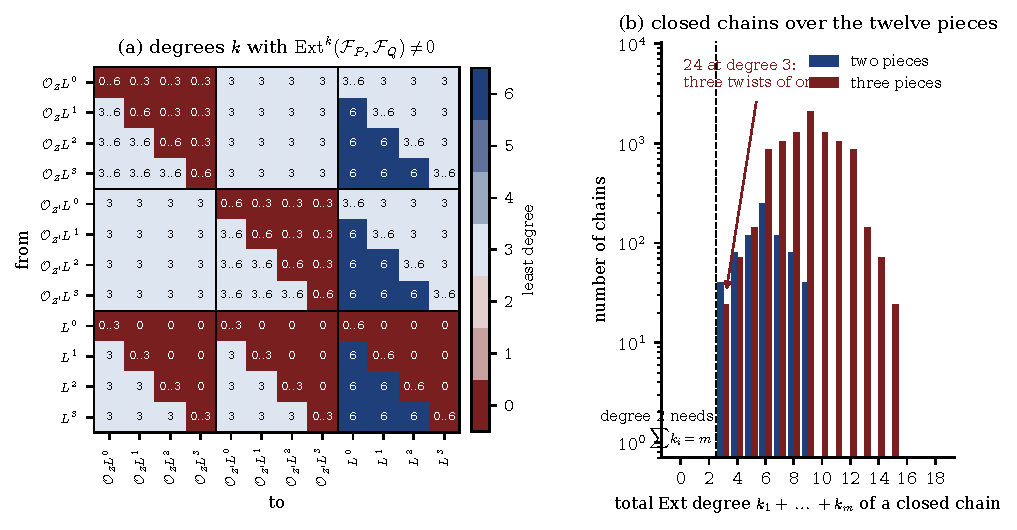
\includegraphics[width=0.96\textwidth]{figures/fig_extgrid}
\caption{The degrees of the Ext groups between the twelve pieces $\mathcal{O}_{Z}L^{k}$, $\mathcal{O}_{Z'}L^{k}$, $L^{k}$, $k=0,\dots,3$, of Table~\ref{tab:cmext}. Left: the degrees in which $\Ext^{k}(\mathcal{F}_{P},\mathcal{F}_{Q})$ is nonzero, coloured by the least one; degree zero occurs only from a lower twist to a higher one and from $L^{a}$ to $\mathcal{O}_{Z}L^{a}$. Right: the number of closed chains of two and of three distinct pieces by total degree, on a logarithmic scale; no two-piece chain has total degree below three, and the three-piece chains of total degree three are those of Proposition~\ref{prop:twostep}.}
\label{fig:extgrid}
\end{figure*}

\begin{figure*}[t]
\centering
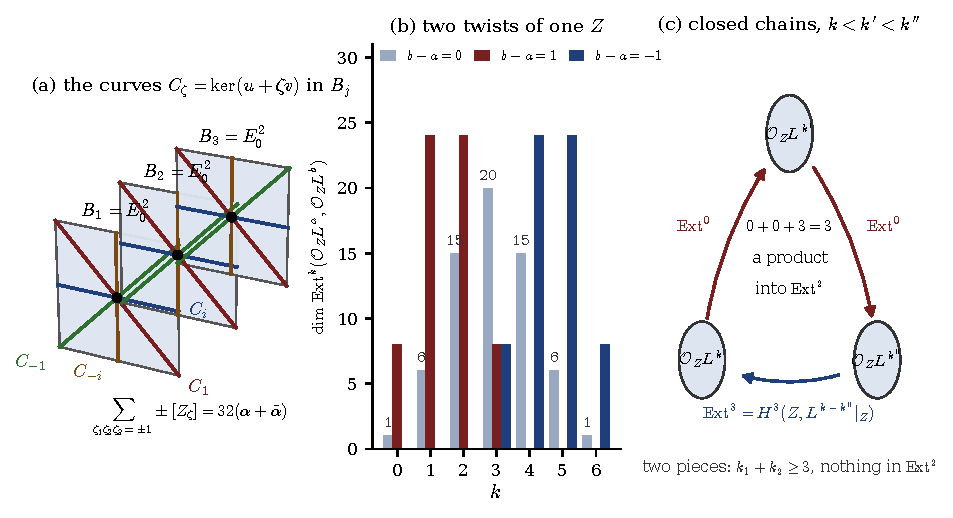
\includegraphics[width=\textwidth]{figures/fig_cmpoint}
\caption{The point $E_{0}^{6}$ of complex multiplication. Left: the three Weil surfaces $B_{j}=E_{0}^{2}$ and the four elliptic curves $C_{\zeta}$ in each, kernels of $u+\zeta v$; a threefold $Z_{\zeta}$ picks one curve in each surface, and the $32$ threefolds with $\zeta_{1}\zeta_{2}\zeta_{3}=\pm1$, signed by that product, add up to $32(\alpha+\bar\alpha)$. Middle: the dimensions of $\Ext^{k}(\mathcal{O}_{Z}\otimes L^{a},\mathcal{O}_{Z}\otimes L^{b})$ by degree for $b-a=0$ (the $\binom{6}{k}$), $b-a=1$ (degrees $0$ to $3$) and $b-a=-1$ (degrees $3$ to $6$). Right: the closed chains of Proposition~\ref{prop:twostep}; every two-step chain has total degree at least three, and the shortest chains reaching degree two run through three twists of one threefold with degrees $0,0,3$.}
\label{fig:cmpoint}
\end{figure*}

\subsection{The forms and the Hodge ring}\label{app:forms}

Write $z_{1},\dots,z_{6}$ for the coordinates of $A_{0}=E_{0}^{6}$, $E_{0}=\CC/\ZZ[i]$, group the factors into the three surfaces $B_{j}=E_{0}^{2}$ with coordinates $(z_{j},z_{3+j})$, $j=1,2,3$, and let $K=\QQ(i)$ act by $i$ on $z_{1},z_{2},z_{3}$ and by $-i$ on $z_{4},z_{5},z_{6}$. Put
\begin{equation}\label{eq:cmforms}
\begin{aligned}
a_{j}&=\tfrac{i}{2}\,dz_{j}\wedge d\bar z_{j}, &
b_{j}&=\tfrac{i}{2}\,dz_{3+j}\wedge d\bar z_{3+j},\\
c_{j}&=\tfrac{i}{2}\,dz_{j}\wedge d\bar z_{3+j}, &
\bar c_{j}&=\tfrac{i}{2}\,dz_{3+j}\wedge d\bar z_{j}.
\end{aligned}
\end{equation}
In the real coordinates $z_{j}=x_{j}+iy_{j}$ one has $a_{j}=dx_{j}\wedge dy_{j}$, the volume form of the $j$-th factor, of integral one over $\CC/\ZZ[i]$,\footnote{The fundamental domain of $\ZZ[i]$ is the unit square, so $\int_{E_{0}}dx\wedge dy=1$; this normalisation makes every form in \eqref{eq:cmforms} integral on the lattice $\ZZ[i]^{6}$, and all intersection numbers below are integers computed as integrals of top forms.} and $c_{j}=\tfrac12(dx_{j}\wedge dy_{3+j}-dy_{j}\wedge dx_{3+j})+\tfrac{i}{2}(dx_{j}\wedge dx_{3+j}+dy_{j}\wedge dy_{3+j})$, so that the real and imaginary parts of $c_{j}$ are rational classes and $\bar c_{j}$ is the complex conjugate of $c_{j}$. All four forms have type $(1,1)$. The polarisation is
\begin{equation}\label{eq:cmtheta}
\theta=\sum_{j=1}^{3}(a_{j}+b_{j}),\qquad \theta^{6}=6!\,a_{1}b_{1}a_{2}b_{2}a_{3}b_{3},\qquad \int_{A_{0}}\frac{\theta^{6}}{6!}=1,
\end{equation}
the principal polarisation of the product; the hermitian forms $\sum_{j\le3}a'_{j}z_{j}\bar w_{j}-\sum_{j>3}a'_{j}z_{j}\bar w_{j}$ of Lemma~\ref{lem:cmext} with all $a'_{j}=1$ give $\theta$ itself.

The Hodge group of $A_{0}$ is the circle acting by $z$ on $H^{1,0}$ and by $\bar z$ on $H^{0,1}$, so the Hodge classes of degree $2k$ are exactly the rational classes of type $(k,k)$, of dimension $\binom{6}{k}^{2}$:
\begin{equation}\label{eq:cmdims}
\dim\Hdg^{2k}(A_{0})=1,\,36,\,225,\,400,\,225,\,36,\,1\quad(k=0,\dots,6).
\end{equation}
In degree two these are the $36$ hermitian forms on $\ZZ[i]^{6}$, the Picard number of $E_{0}^{6}$. The $K$-eigenspaces of $H^{1}(A_{0},\CC)$ are spanned by $dz_{1},dz_{2},dz_{3},d\bar z_{4},d\bar z_{5},d\bar z_{6}$ (eigenvalue $i$) and by their conjugates, so the Weil plane $W=\bigwedge^{6}_{K}H^{1}(A_{0},K)\subseteq H^{6}(A_{0},\QQ)$ is spanned over $\CC$ by
\begin{equation}\label{eq:cmweil}
\alpha=c_{1}c_{2}c_{3}\propto dz_{1}dz_{2}dz_{3}\,d\bar z_{4}d\bar z_{5}d\bar z_{6}\qquad\text{and}\qquad\bar\alpha=\bar c_{1}\bar c_{2}\bar c_{3},
\end{equation}
and over $\QQ$ by $\alpha+\bar\alpha$ and $i(\alpha-\bar\alpha)$. The relation $W\theta=0$ is visible term by term: $c_{j}a_{j}$ contains $dz_{j}$ twice and $c_{j}b_{j}$ contains $d\bar z_{3+j}$ twice, so $\alpha\,(a_{k}+b_{k})=0$ for each $k$, since $\alpha$ already contains $dz_{k}$ and $d\bar z_{3+k}$.

\subsection{The elliptic curves \texorpdfstring{$C_{\zeta}$}{C} and the threefolds \texorpdfstring{$Z_{\zeta}$}{Z}}\label{app:curves}

For $\zeta\in\mu_{4}=\{1,i,-1,-i\}$ let $C_{\zeta}\subseteq B_{j}$ be the kernel of $(u,v)\mapsto u+\zeta v$, an elliptic curve isomorphic to $E_{0}$, and for $\zeta=(\zeta_{1},\zeta_{2},\zeta_{3})\in\mu_{4}^{3}$ let $Z_{\zeta}=C_{\zeta_{1}}\times C_{\zeta_{2}}\times C_{\zeta_{3}}\subseteq A_{0}$, an abelian threefold.

\begin{lemma}\label{lem:cmcurves}
\begin{enumerate}[label=\textup{(\roman*)},leftmargin=2.4em,itemsep=2pt]
\item $[C_{\zeta}]=a_{j}+b_{j}+\bar\zeta\,c_{j}+\zeta\,\bar c_{j}$ in $H^{2}(B_{j})$, and $[Z_{\zeta}]=\prod_{j}[C_{\zeta_{j}}]$.
\item $(C_{\zeta}\cdot C_{\zeta'})=|\zeta-\zeta'|^{2}\in\{0,2,4\}$ on $B_{j}$; $Z_{\zeta}\cap Z_{\zeta'}$ is finite exactly when $\zeta_{j}\ne\zeta'_{j}$ for all $j$, and then $|Z_{\zeta}\cap Z_{\zeta'}|=\prod_{j}|\zeta_{j}-\zeta'_{j}|^{2}\in\{8,16,32,64\}$.
\item $\theta|_{Z_{\zeta}}$ has degree two on each factor, $(\theta|_{Z_{\zeta}})^{3}=48$ and $\chi_{Z_{\zeta}}=8$; in particular $[Z_{\zeta}]\theta\ne0$.
\item Writing $S(\omega)=\sum_{\zeta_{1}\zeta_{2}\zeta_{3}=\omega}[Z_{\zeta}]$ for $\omega\in\mu_{4}$,
\begin{equation}\label{eq:cmgenerating}
\begin{gathered}
\sum_{\omega\in\mu_{4}}\omega^{m}S(\omega)=\prod_{j=1}^{3}T_{m,j},\qquad T_{m,j}=\sum_{\zeta\in\mu_{4}}\zeta^{m}[C_{\zeta}],\\
T_{m,j}=4(a_{j}+b_{j}),\ 4c_{j},\ 0,\ 4\bar c_{j}\quad\text{for }m\equiv0,1,2,3\pmod 4,
\end{gathered}
\end{equation}
and therefore
\begin{equation}\label{eq:cm32}
S(1)-S(-1)=\sum_{\zeta_{1}\zeta_{2}\zeta_{3}=1}[Z_{\zeta}]-\sum_{\zeta_{1}\zeta_{2}\zeta_{3}=-1}[Z_{\zeta}]=32\,(\alpha+\bar\alpha).
\end{equation}
\end{enumerate}
\end{lemma}

\begin{proof}
(i) $C_{\zeta}$ is the fibre over $0$ of the surjective homomorphism $f_{\zeta}\colon B_{j}\to E_{0}$, $w=u+\zeta v$, so $[C_{\zeta}]=f_{\zeta}^{*}[0]$ with $[0]=\tfrac{i}{2}dw\wedge d\bar w$, and
\begin{align*}
dw\wedge d\bar w&=(du+\zeta\,dv)\wedge(d\bar u+\bar\zeta\,d\bar v)\\
&=du\wedge d\bar u+dv\wedge d\bar v+\bar\zeta\,du\wedge d\bar v+\zeta\,dv\wedge d\bar u ,
\end{align*}
which is the formula. A product of subvarieties of the factors has the product class.

(ii) On $B_{j}$ the only nonzero products of two of the four forms are $a_{j}b_{j}$ and $c_{j}\bar c_{j}=\bar c_{j}c_{j}=-a_{j}b_{j}$ (reorder $du\,d\bar v\,dv\,d\bar u$ to $-du\,d\bar u\,dv\,d\bar v$), and $\int_{B_{j}}a_{j}b_{j}=1$. Hence $[C_{\zeta}][C_{\zeta'}]=2-\bar\zeta\zeta'-\zeta\bar\zeta'=|\zeta-\zeta'|^{2}$. Directly: a point of $C_{\zeta}\cap C_{\zeta'}$ has $(\zeta-\zeta')v=0$, so $v$ runs over the kernel of $\zeta-\zeta'$ on $E_{0}$, of order $|\zeta-\zeta'|^{2}$, and $u=-\zeta v$ is then determined. The statement for $Z_{\zeta}$ follows factor by factor.

(iii) $\int_{C_{\zeta}}(a_{j}+b_{j})=\int_{B_{j}}(a_{j}+b_{j})[C_{\zeta}]=2$, since $a_{j}c_{j}$, $a_{j}\bar c_{j}$, $b_{j}c_{j}$, $b_{j}\bar c_{j}$ all repeat a differential. So $\theta|_{Z_{\zeta}}=2(p_{1}+p_{2}+p_{3})$ with $p_{j}$ the point class of the $j$-th factor, $(\theta|_{Z_{\zeta}})^{3}=3!\cdot8=48$, and $\chi_{Z_{\zeta}}=48/6=8$.

(iv) The left side of \eqref{eq:cmgenerating} is $\sum_{\zeta}(\zeta_{1}\zeta_{2}\zeta_{3})^{m}\prod_{j}[C_{\zeta_{j}}]$, which factors as the product of the three sums $T_{m,j}$; these are read off from (i), using $\sum_{\zeta\in\mu_{4}}\zeta^{m}=4$ or $0$ according as $4\mid m$ or not. Then $S(1)-S(-1)=\tfrac12\sum_{\omega}(\omega+\omega^{3})S(\omega)=\tfrac12\bigl(\prod_{j}T_{1,j}+\prod_{j}T_{3,j}\bigr)=\tfrac12(64\alpha+64\bar\alpha)$.
\end{proof}

Equation \eqref{eq:cm32} is the analogue, with abelian threefolds in place of line bundles, of the signed sum of the $32$ line bundles on $E_{0}^{6}$ in \cite[Prop.~18.21]{BMB26}: the $32$ threefolds $Z_{\zeta}$ with $\zeta_{1}\zeta_{2}\zeta_{3}=\pm1$, taken with the sign $\zeta_{1}\zeta_{2}\zeta_{3}$, have classes adding up to $32$ times the real Weil class. Together with three powers of $L$ this is a Chern character of polarised shape and Hankel rank three at $A_{0}$, and by Lemma~\ref{lem:cmext}(i) it is one of the shapes a convolution must realise. Two of these threefolds with $\zeta_{j}=\zeta'_{j}$ for one or two indices $j$ meet along a curve or a surface, so Lemma~\ref{lem:cmext}(ii) does not apply to them and Lemma~\ref{lem:cmmeet} gives their groups; Proposition~\ref{prop:separated} shows that no convolution of these thirty-five pieces meets the criterion. Figure~\ref{fig:cmpoint} draws the curves, the dimensions of the Ext groups and the chains.

\subsection{The dimensions in Lemma~\ref{lem:cmext}}\label{app:extdims}

For the threefolds $Z=Z_{\zeta}$ the numbers of Lemma~\ref{lem:cmext} are explicit. Table~\ref{tab:cmext} lists, for every pair of piece types, the degrees $k$ in which $\Ext^{k}$ is nonzero and its dimension; here $m=b-a$ is the difference of the twists, $\chi_{Z}=8$, $Z'=Z_{\zeta'}$ with $\zeta_{j}\ne\zeta'_{j}$ for all $j$, and $(Z\cdot Z')=\prod_{j}|\zeta_{j}-\zeta'_{j}|^{2}$.



Each row of the table restates the corresponding item of Lemma~\ref{lem:cmext}, with $\chi(L^{m}|_{Z})=m^{3}\chi_{Z}=8m^{3}$ from (iii) above and $\chi(L^{m})=m^{6}\theta^{6}/720=m^{6}$ from \eqref{eq:cmtheta}. Two features of the table drive Proposition~\ref{prop:twostep}. Every group between two pieces of different twist is concentrated in degree $0$, in degree $3$ or $6$, or in the range $0$ to $3$ for two twists of one threefold; and a group in degree at most two between distinct pieces occurs only from a lower twist to a higher one, or from $L^{a}$ to $\mathcal{O}_{Z}L^{a}$. The bookkeeping of the proposition is then the following count. A closed chain of $m$ pieces whose edges have Ext degrees $k_{1},\dots,k_{m}$ carries an $m$-fold product into $\Ext^{\sum k_{i}-m+2}$ of the first piece. For $m=2$ the table gives, for each unordered pair of distinct piece types, the two degrees and their sum:
\begin{equation}\label{eq:cmtwostep}
\begin{array}{lll}
(\mathcal{O}_{Z}L^{a},\mathcal{O}_{Z'}L^{b}) & 3+3 & =6,\\
(\mathcal{O}_{Z}L^{a},\mathcal{O}_{Z}L^{b}),\ b>a & (0\text{ to }3)+(3\text{ to }6) & \ge3,\\
(\mathcal{O}_{Z}L^{a},L^{b}),\ b>a & 3+3 & =6,\\
(\mathcal{O}_{Z}L^{a},L^{b}),\ b<a & 6+0 & =6,\\
(\mathcal{O}_{Z}L^{a},L^{a}) & (3\text{ to }6)+(0\text{ to }3) & \ge3,\\
(L^{a},L^{b}) & 0+6 & =6,
\end{array}
\end{equation}
so no two-step product reaches degree two. For $m=3$ the sum must be $3$ with two edges of degree zero, and the table leaves exactly the ascending chains $\mathcal{O}_{Z}L^{k}\to\mathcal{O}_{Z}L^{k'}\to\mathcal{O}_{Z}L^{k''}$, $k<k'<k''$, closed by the degree-three edge $H^{3}(Z,L^{k-k''}|_{Z})$, of dimension $8(k''-k)^{3}$. The program \path{code/cm_point_ext.py} enumerates the chains of two and three pieces over four twists and two threefolds and confirms both statements, together with the identities of Lemma~\ref{lem:cmcurves}. Figure~\ref{fig:extgrid} shows the table as the matrix of the twelve pieces, and the distribution of the total degree over every closed chain of two and of three distinct pieces: the two-piece chains begin at total degree three, and the twenty-four ordered three-piece chains of total degree three are the eight ascending triples of twists of one threefold, each read from its three starting pieces.

\section{Machine checks}\label{app:checks}

Every finite quantity used in the proofs is recomputed by programs in the archive \cite{BB26code}, and the combinatorial and arithmetic statements among them are also proved in Lean~4. No statement proved in the text rests on these checks; the enumerations of Proposition~\ref{prop:e06count} and Remarks~\ref{rem:sevenbundles}, \ref{rem:efourseven} and \ref{rem:sexticfields} are their output and are stated as such, and the rest guard against slips in the hand computations.

\paragraph{Lean.} The file \path{lean/HodgeClosure.lean} (Lean~4.24.0, no Mathlib) contains sixty-two theorems. Section~1 encodes the eight statements and the rule set of Table~\ref{tab:rules} as data, computes closures by iteration, and proves by evaluation that the closures of $\{\mathrm{F2},\mathrm{F3}'\}$, $\{\mathrm{F3}\}$, $\{\mathrm{L},\mathrm{M}\}$, $\{\mathrm{L},\mathrm{F3}'\}$ and $\{\mathrm{V},\mathrm{F3}'\}$ contain $\HC$, that the closures of $\{\mathrm{F2}\}$, $\{\mathrm{F3}'\}$, $\{\mathrm{L}\}$, $\{\mathrm{M}\}$, $\{\mathrm{V}\}$, $\{\AB\}$, $\{\mathrm{L},\mathrm{V}\}$ and $\{\mathrm{M},\mathrm{F3}'\}$ do not, and that the list of minimal sufficient sets, computed from the rule set alone, has exactly six members, those of Proposition~\ref{prop:minimal}. Section~2 works in $\ZZ[\sqrt{-d}]$ and proves that the hermitian form $\eta$ transforms under $\tau$ by $N(\tau)$, that the norm is multiplicative, that $\eta$ is not $K^{\times}$-invariant, and that the characters $N(\tau)^{n}$ and $\tau^{2n}$ differ at explicit $\tau$ (Section~\ref{sec:earlier}). Section~3 proves the dimension counts of Section~\ref{sec:f2}: $3n<n^{2}$ for $n\ge4$, $m^{2}+m'^{2}<(m+m')^{2}$ for $m,m'\ge1$ with $2mm'$ mixed directions, the values $r=57$ and $104$ of the lower bound, and the Hodge class count $26$ of Theorem~\ref{thm:link}(i) as a sum of K\"unneth contributions. Section~4 proves the polynomial identities behind the Fricke families of Section~\ref{ssec:fricke}: $c_{4}^{3}-c_{6}^{2}=1728\,t\,(t^{2}+13t+49)^{2}$ at level $7$ and $1728\,t\,(t^{2}+22t+125)^{3}$ at level $5$, by exact arithmetic on coefficient lists, together with the root products $7^{2}$ and $5^{3}$, the Euler numbers $12$ and $24$, the Shioda--Tate counts giving Picard number at least $16$, the transcendental rank $6$, the dimensions $(n+1)/2$ of the dihedral Hecke algebras, and the polynomial identity behind the sign of Lemma~\ref{lem:frickesign}: with $A'$, $B'$ the V\'elu coefficients of the quotient of \eqref{eq:fricke} by $C_{t}$, computed from the kernel polynomial by Newton's identities on coefficient lists, and $\tilde A(t)=t^{4}A(N^{k}/t)$, $\tilde B(t)=t^{6}B(N^{k}/t)$, the identity $N^{k-1}B'\tilde A+A'\tilde B=0$ holds at both levels, which is $\lambda(t)^{2}=-t^{2}/N^{k-1}$. Section~5 proves the Dickson identities $p_{7}(t+t^{-1})=t^{7}+t^{-7}$ and $p_{9}(t+t^{-1})=t^{9}+t^{-9}$ behind the families of Theorem~\ref{thm:zeta9}, that $2$ has order three in $(\ZZ/7)^{\times}/\pm1$ and in $(\ZZ/9)^{\times}/\pm1$, so that $2$ is inert in both cubic fields, and the sign pattern of the conjugates of $\theta$ at the three real places. Section~6 proves the finite statements of Appendix~\ref{app:cmpoint}: the binomial identity $\sum_{q}\binom{3}{q}\binom{3}{k-q}=\binom{6}{k}$, the intersection numbers $(C_{\zeta}\cdot C_{\zeta'})=|\zeta-\zeta'|^{2}$ and $\theta\cdot C_{\zeta}=2$ in the basis of the $(1,1)$-forms of $B_{j}$ with the pairing $a_{j}b_{j}=1$, $c_{j}\bar c_{j}=-1$, the twisted sums $T_{m,j}$, the identity $S(1)-S(-1)=32(\alpha+\bar\alpha)$ as an equality of the $64$ coefficients of the triple products over $\ZZ[i]$, the counts $48$, $8$, $75$ and $18$ with the Euler characteristics, and the two chain statements of Proposition~\ref{prop:twostep} over the twelve pieces of Appendix~\ref{app:extdims}, each by \texttt{decide}. Section~7 encodes the pieces of Table~\ref{tab:e06count} and the Ext dimensions of Lemmas~\ref{lem:cmext} and \ref{lem:cmmeet}, and proves that the isolated blocks of Lemma~\ref{lem:isolated} sum to $7213$, $2605$, $2605$, $0$, $0$ and $5325$ at the six configurations named in the table; the reachability relation along blocks of total degree one is supplied as a certificate, which the kernel checks to be reflexive, to contain every such block and to be closed under one more step, before the sum is evaluated by \texttt{decide\,+kernel}. From the same certified relation it proves that the configurations (a) and (c) of the table have $32$ and $22$ threefold pieces outside every directed cycle of the graph $\Gamma$ of Section~\ref{ssec:e06count}; and, by evaluating the Ext dimensions on every pair, that no edge of $\Gamma$ enters a piece at shift $1$ from the thirty-two pieces or from the pieces $\mathcal{O}_{Z_{\zeta}}\otimes L^{k}[t]$, $\zeta\in\mu_{4}^{3}$, $1\le k\le3$, and $L^{l}[t]$, $1\le l\le4$, with $-3\le t\le2$, that $L^{1}[3]$, $L^{4}[3]$ and $\mathcal{O}_{Z_{(1,1,1)}}\otimes L^{1}[3]$ do enter, and that $L^{1}[-2],\dots,L^{6}[3]$ put each of the thirty-two pieces on a cycle of length six. Every theorem is checked by \texttt{\#print\,axioms}: fifty-two use no axiom, the two inequalities proved with the arithmetic tactic use \texttt{propext} and \texttt{Quot.sound}, and the six isolated-block counts and the two chain-free counts of Section~7 use \texttt{propext}; \texttt{native\_decide} is not used.

The Lean certificate of \cite{BMB26}, \texttt{HodgeObstruction.lean} (Lean~4.34.0, \leancount{} theorems, each axiom-free or depending on \texttt{propext} only), carries the finite computations of that paper; it is cited and not repeated here. The reduction of Section~\ref{sec:reduction} uses only the hand-proved parts of \cite{BMB26}.

\paragraph{Python.} \path{code/sqrt6_chain.py} (sympy) implements Hilbert symbols and Hasse invariants exactly, verifies the product formula on random pairs, classifies $U_{\QQ}$, $E_{8}(-1)_{\QQ}$ and the invariant lattices, reproduces Varesco's embedding results for $\sqrt2$ and $\sqrt3$ as controls, searches the $165$ sign-admissible small forms $q_{E}$ over $\QQ(\sqrt6)$ ($98$ embed in $V_{3}$, $67$ do not), exhibits the complements $\langle1,-10\rangle$ and $\langle1,-1,-1,-1,-3,-30\rangle$, and checks both orders of the chain: twenty-five checks. \path{code/fricke_families.py} computes the fibre types, Euler numbers and Picard bounds of the Fricke curves and their twists at levels $5$ and $7$, checks numerically that the roots of $j(t)=j(\tau)$ are carried by $t\mapsto N^{k}/t$ to the $j$-invariants of the $N$-isogenous curves, verifies the twist identity $u_{p,q}(w(t))=pq\,u_{w(p),w(q)}(t)/t^{2}$, the M\"obius transformations preserving the labelled points, the embedding of every rank-six form of signature $(2,4)$ in $V_{2}$ and $V_{3}$ after any scaling, and the Hecke algebras of $(D_{n},\langle\tau\rangle)$ for $n=5,7,9,11$: forty-one checks. \path{code/product_object.py} builds the exterior-algebra model of $H^{*}(A\times A')$ for $(m,m')=(2,1),(2,2)$, the tangent space of $\cD_{n,n}$ and of the product locus, the first-order Hodge loci of the exterior products and of the object of Theorem~\ref{thm:product}, the Vandermonde determinant, the vanishing of the cross terms, and the Hankel rank and $r(\gamma)$ of the final class; \path{code/convolution_checks.py} computes in the same model the rank of $v\mapsto v\lrcorner\theta_{A}$ on $T\cD_{n,n}$, the contraction ranks of $\ch(\mathcal{E}')$ and $\ch(\mathcal{E}'')$ in Proposition~\ref{prop:convolution}(iii), and the trace of an upper triangular times a strictly upper triangular block matrix. In these two programs ranks are computed in floating point with a relative tolerance of $10^{-7}$ and agree with the closed formulas. \path{code/sixfold_link.py} checks the alternation and invariances of $\psi_{c}$, the decomposition of the $K^{1}$-invariants, the ratio of the induced forms at the three places, the symmetry of $T_{X}(-1)$, the count $26$ and the weight support of $\xi$; \path{code/link_weights.py} computes the Hodge classes of degree four on $X\times X\times Z_{K}$ under the three groups of Section~\ref{ssec:f2stop2} and the vanishing of $\Hom(X_{c},Z_{K,c})$ at the compositum CM point. \path{code/zeta9_invariants.py} computes the rank, signature, discriminant and Hasse invariants of the trace form $\Tr_{F/\QQ}(-\theta\,\mathrm{nrd})$ on the quaternion algebra $(-1,-\theta)_{F}$, $F=\QQ(\zeta_{9})^{+}$, and of the transcendental lattice of the dihedral family of Theorem~\ref{thm:zeta9} for $n=9$, and checks that they agree while three contrasting algebras fail; \path{code/zeta7_invariants.py} does the same for $n=7$, with $(-1,\theta)_{F}$, $F=\QQ(\zeta_{7})^{+}$, the lattice $U^{2}\oplus E_{8}(-1)$ and the competing algebras ramified at $7$ or $43$, and checks the Dickson identity of \eqref{eq:dickson7}; \path{code/annihilator_exact.py} verifies in exact arithmetic over $\QQ(\sqrt{-3})$, at $(m,m')=(2,1)$ and $(2,2)$, the formula \eqref{eq:chEprime} and the dimension $m^{2}+m'^{2}$ of the annihilator in Theorem~\ref{thm:annihilator}, component by component; \path{code/riemann_roch_pieces.py} computes the polynomial \eqref{eq:rrpoly} and the thirty-one supports of Proposition~\ref{prop:noorth}; \path{code/cm_point_ext.py} checks Lemma~\ref{lem:cmext} and Proposition~\ref{prop:twostep}: the identity $\sum\binom{3}{q}\binom{3}{p}=\binom{6}{k}$, the Koszul cohomology of a transverse intersection in exact arithmetic, the Euler characteristics of the twisted groups, the enumeration of the closed chains of two and three pieces with their degrees, and the identities of Lemma~\ref{lem:cmcurves} in the exterior algebra of the twelve real one-forms of $E_{0}^{6}$; \path{code/cm_point_counts.py} enumerates the configurations of Table~\ref{tab:e06count}, computes their Chern characters exactly in the Hodge ring of $E_{0}^{6}$, and recomputes for each the sums $C^{1},C^{2},C^{3}$, the Euler characteristic and the isolated blocks of Lemma~\ref{lem:isolated}; \path{code/cm_point_chains.py} builds the graph $\Gamma$ of Section~\ref{ssec:e06count} from the same dimensions, finds its directed cycles through the strongly connected components, and checks the statements of Remark~\ref{rem:chainfreecount} together with the absence of closed chains among the thirty-five pieces of Proposition~\ref{prop:separated}. \path{code/line_bundle_chains.py} builds, for every arrangement of the shifts of $n\le8$ line bundles forming an interval, the graph of up, down and run edges, with a run table derived from the degrees of Lemmas~\ref{lem:cmext} and \ref{lem:cmmeet}, applies the rules of Proposition~\ref{prop:effective} and Lemma~\ref{lem:mcrules} over every set of vanishing up edges, and reports the counts of Remark~\ref{rem:sevenbundles}, with the ranks $\sum_{i}(-1)^{t_{i}}$ of the thirty-one arrangements of eight: five checks. \path{code/threefold_supports.py} checks the exact arithmetic of Section~\ref{ssec:supports}: the entries of the vectors of $T\cD_{h}$ and the restrictions $\kappa_{T}(v)_{k}|_{\Gamma_{y}}$, $\kappa_{T'}(v)_{k}|_{\Gamma'_{y}}$ of Theorem~\ref{thm:pair} for every $\zeta$ and every pair $j\ne k$, the four points of $C_{\zeta_{j}}\cap C_{-\zeta_{j}}$ and the coordinates $n'_{j}|_{\Gamma_{y}}=n_{j}|_{\Gamma'_{y}}=2z_{j}$, the threefolds meeting a general $\Gamma_{y}$ (Lemma~\ref{lem:curvesT}), the coefficients $\sigma(x)\prod_{\varepsilon_{j}=1}c(x)_{j}$ of $X_{\varepsilon}$ in $[Z_{x}]$ and the Fourier inversion of Lemma~\ref{lem:orbits}, the vanishing of $\theta_{h}X_{\varepsilon}$ and the absence of the weights $\pm2\varepsilon$ from $H^{4}(A_{0})$, and for Lemma~\ref{lem:fourline} and Theorem~\ref{thm:sixtyfour} the values $dn_{a}(v)$, $dn_{k}(v)$, $dn_{l}(v)$ at $Y=E_{jk}$, the classes $[C_{a}]\wedge d\bar z_{3+j}$ and the two relations they impose, the solutions $\mu_{a}=m\,a^{2}$ of the relations, the intersection numbers $Q\cdot C_{b}=8$ and $Q^{2}=32$ and the finiteness of $C_{1}\cap C_{i}$, the threefolds meeting $Q\times\{y\}$ for general $y$, the passage from the relations along the lines to $\mu_{x}=m\,\sigma(x)^{2}$, and the vanishing $\sum_{x}\sigma(x)^{2}[Z_{x}]=0$: sixteen checks. \path{code/kummer_type.py} implements the Hasse invariants and the criterion (c) of Proposition~\ref{prop:kummerq}, compares it on fourteen quadratic spaces of ranks four and five with a direct search for a complement $W$ with $T\oplus W\cong U_{\QQ}^{3}$ by the invariants of Hasse--Minkowski, computes the discriminants of $U_{\QQ}^{3}$, of the transcendental spaces of the Fricke surfaces and of the two families of \cite{Var25}, names the primes at which the failing examples of Remark~\ref{rem:detfrontier} fail, and counts the spaces of ranks four and five with coefficients in $\pm\{1,2,3,5,6,10,15,30\}$ that meet the condition ($1084$ of $1296$ and $1304$ of $4320$). \path{code/fricke_sign.py} (sympy) computes the $N$-th division polynomial of \eqref{eq:fricke} over $\ZZ[t,x]$, isolates the factor of degree $(N-1)/2$ that is the kernel polynomial of $C_{t}$, applies V\'elu's formulas, checks that the quotient has the $j$-invariant of $\mathcal{E}_{w(t)}$, computes $\lambda(t)^{2}=-t^{2}/25$ and $-t^{2}/7$, the products $\lambda(t)\lambda(w(t))=\pm N$ with the sign fixed by the analytic model of Lemma~\ref{lem:frickesign}, the twist constants $c(t)c(w(t))=1$ and $-1$ and the resulting $\Lambda^{2}=-N$ and $N$, the identity checked in Lean, and the composite $f_{w(\tau)}\circ f_{\tau}=[-N]$ with kernel $\langle1/N\rangle$ in the analytic model: thirty-two checks. \path{code/fricke_picard.py} counts the points of $X_{1}$ over $\mathbb{F}_{\ell^{i}}$, $i\le3$, for $\ell=11$ at level $7$ and $\ell=7$ at level $5$, in exact arithmetic with Zech logarithms, forms the traces of Frobenius on the rank-six complement of the trivial lattice, completes the characteristic polynomial by Newton's identities and the functional equation, checks that the sign of the functional equation is determined, that the polynomial has integer coefficients, is irreducible over $\QQ$, splits over $\QQ(\sqrt{-N})$ into a cubic and its conjugate and has no cyclotomic factor after the normalisation $x\mapsto\ell x$, that the odd traces vanish at the inert primes $5$ and $11$, and that the same counts on the rational surfaces $R_{N}$ give the traces of a rational elliptic surface: twelve checks. \path{code/fricke_lattice.py} recomputes, by the same invariants, the rational isometries $A_{n}\oplus\langle n+1\rangle\cong\langle1\rangle^{n+1}$, $D_{4}\cong\langle1\rangle^{4}$, $A_{1}^{2}\cong\langle1\rangle^{2}$, $E_{8}\cong\langle1\rangle^{8}$ of the proof of Proposition~\ref{prop:frickeks}(i), the isometries $T\cong U_{\QQ}^{2}\oplus\langle-1\rangle\oplus\langle-N\rangle$ for $N=5,7$ both by cancellation and from the invariants of the K3 lattice and of $M$, the pairs $(a,b)$ with $U_{\QQ}^{2}\oplus\langle a,b\rangle\cong T$ in a box, the signed discriminant $-N$, and the dimension count of the Hodge groups: twenty-one checks. \path{code/closure_graph.py} recomputes the closures and the minimal sets, and \path{code/bypass_checks.py} the Horn closure with the facts of the literature on abelian varieties adjoined and the blow-up bookkeeping of Proposition~\ref{prop:bypass}(ii). \path{code/cover_boundary.py} (sympy) checks the smoothness of $B_{\lambda}$, the divisor of $y^{3}+1/\lambda$, the nontriviality of $\eta$ and the rank nine of the multiplication map of Proposition~\ref{prop:genusfour}. \path{code/sextic_cubic_fields.py}, with \path{code/sextic_lattice.py} from the archive of \cite{BMB26}, computes in exact arithmetic the lattices of integral points of $S(0,q)$ of Remark~\ref{rem:sexticfields} over the twelve cubic fields, their Gram matrices and their short vectors. \path{code/efour_seven.py} (numpy, scipy) recomputes exactly the weights and the largest nontrivial character sums of the weighted Cayley graphs of Section~\ref{ssec:efourseven} and runs the linear programs of Remark~\ref{rem:efourseven} over every distribution of the pieces in the twelve arrangements, in double precision.

\paragraph{Julia, C, C\texttt{++} and shell.} \path{code/closure_graph.jl}, \path{code/closure_graph.c} and \path{code/closure_graph.cpp} recompute the closures of all $256$ subsets of the eight statements and the six minimal sets by three independent implementations of the fixed-point iteration; \path{code/eigencharacter.jl} recomputes the characters of Section~\ref{sec:earlier} in exact integer arithmetic, and \path{code/hilbert.c} the Hilbert symbols and the invariants of Table~\ref{tab:invariants}; \path{code/run_all.sh} runs every program and the Lean file and prints a line per check. The expected outputs are recorded in \path{code/EXPECTED.md}.


\section{Exact tensor operations and the limits of character constructions}
\label{v7:app:derivations}

This appendix records the finite calculations used in the new sections.
The calculations check identities in representations and in rational
$K$-theory. They do not decide whether a Hodge class on a general fibre
has an algebraic representative.

\subsection{The cube of weights and its two determinant tensors}

The eight weights of the matched fourfold are the vertices of a cube.
The two sets of four vertices in Figure~\ref{v7:fig:cube} are exchanged
by the conjugation of $k$. The columns of the matrix
\[
 W=\begin{pmatrix}
 1&1&-1&-1\\1&-1&1&-1\\1&-1&-1&1
 \end{pmatrix}
\]
are $w_1,w_2,w_3,w_4$. The first three columns have determinant $4$,
and $W(1,1,1,1)^{\mathsf t}=0$. Hence the integral kernel of $W$ is
exactly $\ZZ(1,1,1,1)$. If a zero-weight multiset has multiplicities
$a_i,b_i$ at $w_i,-w_i$, its difference vector is therefore a constant
integer vector. Removing $\min(a_i,b_i)$ opposite pairs at each vertex
leaves whole copies of one tetrahedron. This proves the multiset
assertion for every tensor degree, rather than only the degrees
enumerated by a program.

\begin{figure}[htbp]
\centering
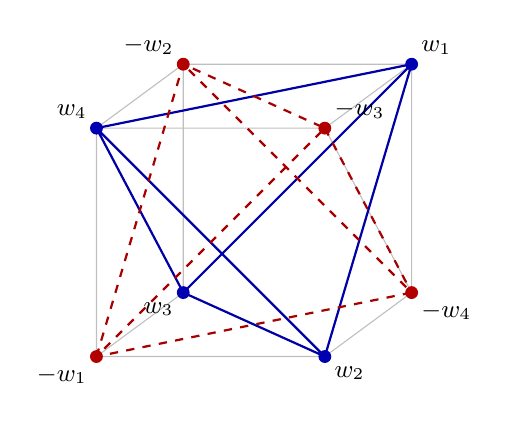
\begin{tikzpicture}[scale=1.45,font=\small]
 \coordinate (a) at (1.38,1.28);
 \coordinate (b) at (.62,-1.28);
 \coordinate (c) at (-.62,-.72);
 \coordinate (d) at (-1.38,.72);
 \coordinate (A) at (-1.38,-1.28);
 \coordinate (B) at (-.62,1.28);
 \coordinate (C) at (.62,.72);
 \coordinate (D) at (1.38,-.72);
 \draw[gray!50] (a)--(B)--(d)--(C)--(a)--(D)--(b)--(A)--(d);
 \draw[gray!50] (A)--(c)--(B) (c)--(b) (C)--(D);
 \draw[blue!65!black,thick] (a)--(b)--(c)--(a)--(d)--(b) (c)--(d);
 \draw[red!65!black,dashed,thick] (A)--(B)--(C)--(A)--(D)--(B) (C)--(D);
 \foreach \p in {a,b,c,d}{\fill[blue!70!black] (\p) circle(1.6pt);}
 \foreach \p in {A,B,C,D}{\fill[red!70!black] (\p) circle(1.6pt);}
 \node[above right] at (a) {$w_1$};
 \node[below right] at (b) {$w_2$};
 \node[below left] at (c) {$w_3$};
 \node[above left] at (d) {$w_4$};
 \node[below left] at (A) {$-w_1$};
 \node[above left] at (B) {$-w_2$};
 \node[above right] at (C) {$-w_3$};
 \node[below right] at (D) {$-w_4$};
\end{tikzpicture}
\caption{A projection of the weight cube. Opposite pairs and the two
tetrahedra generate every zero-weight multiset. The picture describes
the representation at the matched CM fibre; it does not identify
cycles on a generic Mumford fibre.}\label{v7:fig:cube}
\end{figure}

On a power of the fourfold there can be many copies of a weight.
To separate their slots, choose rational endomorphisms on the source
factors and use maps $(x_1,\ldots,x_m)\mapsto\sum f_j(x_j)$.
After scalar extension the endomorphism algebra contains the
individual weight projectors. The pullback of a tetrahedron then
has independently variable coefficients at its four slots.
Coefficient extraction, or a Vandermonde interpolation using rational
parameters, spans every choice of four slots. A polynomial vanishing
on all rational parameters vanishes identically. This explains why
the weight calculation proves generation on all powers, rather than
only on the fourfold itself.

\subsection{Partial symplectic transpose}

In the ordered basis $e\otimes e,e\otimes f,f\otimes e,f\otimes f$
the swap on a two-dimensional factor has matrix
\[
 S=\begin{pmatrix}1&0&0&0\\0&0&1&0\\0&1&0&0\\0&0&0&1\end{pmatrix}.
\]
Write $J=\left(\begin{smallmatrix}0&1\\-1&0\end{smallmatrix}\right)$
for the alternating form. If $t_1$ is ordinary transpose in the first
factor, define
\[
 \tau(A)=(J^{-1}\otimes I)A^{t_1}(J\otimes I).
\]
Direct matrix multiplication gives $\tau(S)=I-S$ and
$\tau((I-S)/2)=S/2$. For a product of operators in the three distinct
colours the transpose factors colour by colour. It is not an algebra
homomorphism on arbitrary endomorphisms, and no such assertion is used.
On the common eigenspace of the three swaps with signs
$\epsilon_i,\epsilon_j,\epsilon_l$, the adjoint projector gives
\[
 \tau(P_i)=\left(1-\frac{\epsilon_i}{2}\right)
            \frac{\epsilon_j\epsilon_l}{4}.
\]
Its square is $1/64$ for $\epsilon_i=1$ and $9/64$ for
$\epsilon_i=-1$, proving the interpolation in
Theorem~\ref{v7:thm:powers}.

For the primitive projector from $\bigwedge^2V$, the corresponding
eigenvalue is
\[
 \frac{\epsilon_i}{2}
  \left(1-\frac{\epsilon_j}{2}\right)
  \left(1-\frac{\epsilon_l}{2}\right).
\]
Its possible values are $\pm1/8,\pm3/8,\pm9/8$.
A polynomial taking value $1$ at the negative values and $0$ at the
positive values recovers $(1-s_i)/2$. The six values are distinct,
so rational Lagrange interpolation supplies this polynomial. Every
coefficient is rational before the scalar extension that separates
the three embeddings of $F$.

\begin{figure}[htbp]
\centering
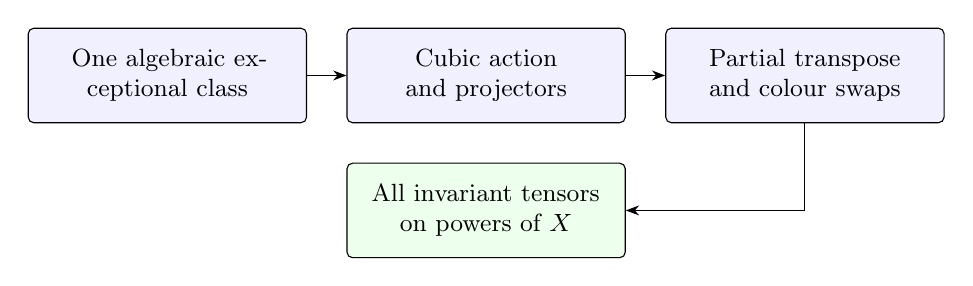
\begin{tikzpicture}[>=Stealth,node distance=5mm,font=\small,
 b/.style={draw,rounded corners=2pt,text width=33mm,minimum height=12mm,align=center}]
 \node[b,fill=blue!6] (a) {One algebraic\ exceptional class};
 \node[b,right=of a,fill=blue!6] (b) {Cubic action\ and projectors};
 \node[b,right=of b,fill=blue!6] (c) {Partial transpose\ and colour swaps};
 \node[b,below=of b,fill=green!7] (d) {All invariant tensors\ on powers of $X$};
 \draw[->] (a)--(b); \draw[->] (b)--(c);
 \draw[->] (c.south)|-(d.east);
\end{tikzpicture}
\caption{An explicit conditional transfer. The tensor operations are
algebraic; the first exceptional cycle is the missing input at a
full-group fibre.}\label{v7:fig:transfer}
\end{figure}

\subsection{Why a pure mixed character is not an effective sheaf}

Let $Y=X_c^2\times Z_c$, and let $H$ be the sum of ample classes
pulled back from its three factors. Its dimension is fourteen.
The nonzero mixed class $\xi_c$ has K\"unneth degrees $(1,1,2)$,
whereas every term of $H^{12}$ has even degree on each factor.
Integration over $Y$ therefore gives
\begin{equation}\label{v7:eq:zero-degree}
 \int_Y \xi_c H^{12}=0.
\end{equation}

\begin{proposition}\label{v7:prop:no-effective-pure}
The perfect complex in Proposition~\ref{v7:prop:adams} cannot be
replaced by a coherent sheaf with the same cohomological Chern
character. Nor can a vector bundle with character $r+N\xi_c$, with
$r,N>0$, admit a Hermite--Einstein metric for the product polarization
$H$.
\end{proposition}
\begin{proof}
Suppose a coherent sheaf has $\ch_0=\ch_1=0$ and
$\ch_2=N\xi_c\ne0$. Rank zero makes it torsion. Its codimension-one
cycle is effective and represents $\ch_1$. Positivity of degree for
an ample polarization forces that cycle to vanish, so the support
has codimension at least two. Its leading codimension-two cycle is
again effective, with positive lengths at its generic points, and
represents $\ch_2$. If nonzero it has strictly positive intersection
with $H^{12}$, contradicting \eqref{v7:eq:zero-degree}. If it is zero,
then $\ch_2=0$, also a contradiction.

For a rank-$r$ bundle with the indicated character, $c_1=0$ and
$2r c_2-(r-1)c_1^2=-2rN\xi_c$. Its intersection with $H^{12}$ is
zero. In the Chern--Weil equality for a Hermite--Einstein connection
this intersection is a positive constant times the squared norm
of the trace-free curvature \cite{Lub82}. It follows that the
connection is projectively flat. A projectively flat bundle has
$\ch_2=c_1^2/(2r)$, which is zero here, contradicting
$\ch_2=N\xi_c\ne0$.
\end{proof}

Thus clearing denominators and applying Adams operations construct
a perfect complex but do not produce a positive sheaf or a
Hermite--Einstein representative. A construction using stability has
to change the other Chern components as well and check their Hodge
behaviour. This is an obstruction to these particular representatives,
not to algebraicity of the mixed cycle.

\subsection{The character projection and the deformation obstruction}

For $0\le j\le14$, Adams operations act on $\ch_j$ by $2^j$.
The polynomial
\[
 q_2(T)=\prod_{\substack{0\le j\le14\\j\ne2}}
        \frac{T-2^j}{4-2^j}
\]
satisfies $q_2(4)=1$ and $q_2(2^j)=0$ for every other $j$ in this
range. Its coefficients can be checked in $\QQ$ without a cycle
oracle. The construction controls the image in cohomology of a
$K$-class. Deformation of an object representing that class is
governed instead by its Atiyah class and self-extension groups.

\begin{figure}[htbp]
\centering
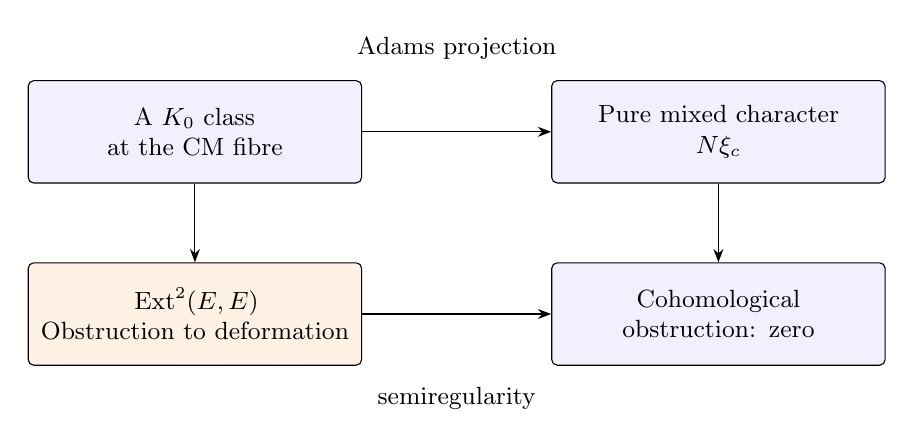
\begin{tikzpicture}[>=Stealth,node distance=24mm,font=\small,
 b/.style={draw,rounded corners=2pt,text width=40mm,minimum height=13mm,align=center}]
 \node[b,fill=blue!6] (k) {A $K_0$ class\\at the CM fibre};
 \node[b,right=of k,fill=blue!6] (ch) {Pure mixed character\\$N\xi_c$};
 \node[b,below=10mm of k,fill=orange!10] (ext) {$\operatorname{Ext}^2(E,E)$\\Obstruction to deformation};
 \node[b,right=of ext,fill=blue!6] (h) {Cohomological\\obstruction: zero};
 \draw[->] (k)--node[above=8mm]{Adams projection}(ch);
 \draw[->] (k)--(ext); \draw[->] (ch)--(h);
 \draw[->] (ext)--node[below=8mm]{semiregularity}(h);
\end{tikzpicture}
\caption{The bottom arrow can have a nonzero kernel. The explicit K3
example of Theorem~\ref{v7:k3-obstructed-bundle} exhibits a
nonzero obstruction in that kernel despite preservation of the
entire Chern character.}\label{v7:fig:obstruction}
\end{figure}

The file \path{checks/check_weights.py} verifies the subset counts
for $\bigwedge^3V$ and $\bigwedge^4V$, the matched CM weight
multiset, the two-dimensional partial-transpose matrix identities,
all fifteen Adams eigenvalues, and the ranks of the root
intertwining systems. All arithmetic in that file is exact.
The infinite-degree multiset argument, the existence of the CM
embedding, the algebraic projector construction and the deformation
arguments are proved in the text. The finite checks neither
formalise those geometric proofs nor establish \Fii{} or \Fiii{}.


\section{Matrix reconstruction and the two obstruction quotients}
\label{v7:app:matrix-reconstruction}

The new arguments use algebraic correspondences and finite matrix
identities in distinct ways. We record the identities so that the
computations have a precise scope. They check the displayed linear
algebra, not the existence of the missing cycles.

\subsection{The two-stage obstruction}

For every smooth projective \(X\), the inclusions
\(\Alg^p(X)\subseteq\Ab^p(X)\subseteq\Hdg^p(X)\) give
the exact sequence
\begin{equation}\label{v7:eq:two-stage-exact}
0\longrightarrow\frac{\Ab^p(X)}{\Alg^p(X)}
 \longrightarrow D_{\Alg}^p(X)
 \longrightarrow D_{\Ab}^p(X)\longrightarrow0.
\end{equation}
The first map is induced by inclusion, so is injective. The second
sends the coset of \(\alpha\) modulo \(\Alg\) to its coset modulo
\(\Ab\); it is surjective, and its kernel consists exactly of
classes in \(\Ab\) modulo \(\Alg\). This proves exactness without
choosing a splitting. All three maps commute with algebraic
correspondences.

Every class in the left term is a finite sum of images of classes in
\(D_{\Alg}(A)\), where \(A\) is abelian: use the defining expression
\(\sum\Gamma_{i*}\beta_i\) for \(\Ab\), and pass to the quotient.
Replacing \(\beta_i\) by an algebraic class changes its image by an
algebraic class, so these quotient maps are well defined. Universal
\Fii{} makes every such source quotient zero; it therefore kills
the left term. Universal \Fiii{} kills the right term. Their
conjunction kills the middle term, which is the rational Hodge
conjecture. This is a description of the two obligations, not a
proof that either quotient vanishes.

\begin{figure}[ht]
\centering
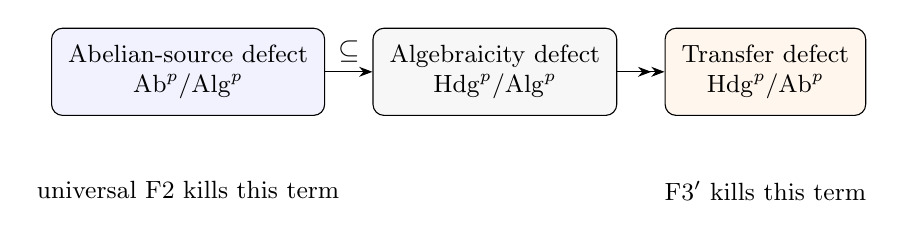
\begin{tikzpicture}[>=Stealth,node distance=6mm,
 box/.style={draw,rounded corners,align=center,inner sep=6pt,font=\small}]
\node[box,fill=blue!5] (a) {Abelian-source defect\\\(\Ab^p/\Alg^p\)};
\node[box,fill=gray!6,right=of a] (b) {Algebraicity defect\\\(\Hdg^p/\Alg^p\)};
\node[box,fill=orange!7,right=of b] (c) {Transfer defect\\\(\Hdg^p/\Ab^p\)};
\draw[->] (a)--node[above]{\(\subseteq\)}(b);
\draw[->>] (b)--(c);
\node[below=7mm of a,font=\small] {universal F2 kills this term};
\node[below=7mm of c,font=\small] {F3\( {}'\) kills this term};
\end{tikzpicture}
\caption{The exact sequence \eqref{v7:eq:two-stage-exact}.
The middle obstruction vanishes when both outer terms vanish.
The diagram does not assert that they already vanish.}
\label{v7:fig:two-defects}
\end{figure}

\subsection{The projector matrix}

Write \(v_i=hD_i\), and let
\(\ell_j(\alpha)=\int_X\alpha D_jh^{d-3}\). Then
\(\ell_j(v_i)=Q_{ji}\). If \(V\) is the column matrix with
columns \(v_i\) and \(L\) has rows \(\ell_j\), then
\[
 LV=Q,\qquad P=VQ^{-1}L,\qquad
 P^2=VQ^{-1}(LV)Q^{-1}L=P.
\]
Moreover \(PV=V\), \(L(1-P)=0\), and \(P(1-P)=0\).
These identities give the coefficient extraction and the complementary
projection in Proposition~\ref{v7:prop:primitive-hodge-projector}.
The proof of that proposition identifies the complement with primitive
classes on \(\Hdg^2(X)\).\footnote{The finite identities alone
would only identify \(\ker L\). The hard Lefschetz argument on
Hodge classes is what identifies that kernel with the primitive
Hodge subspace. No claim about the full non-Hodge cohomology follows
from the finite matrix test.}

For the completely numerical model
\[
 Q=\begin{pmatrix}4&1\\1&-2\end{pmatrix},\qquad
 Q^{-1}=\frac19\begin{pmatrix}2&1\\1&-4\end{pmatrix},
\]
take \(V\) to be the first two coordinate vectors of \(\QQ^4\)
and \(L=(Q\mid 0)\). Then \(P=\operatorname{diag}(1,1,0,0)\).
The last two coordinates model a remaining quotient; the example
does not identify them with classes on an actual variety.

\subsection{Triangular recovery and traces}

The projective-bundle coefficient equations have upper triangular
matrix \(T\) with entries \(T_{jk}=u_{k-j}\) for \(k\ge j\),
\(T_{jj}=1\), and zero for \(k<j\). If \(N=T-I\), then
\(N^{r+1}=0\), and the exact inverse is
\[
 T^{-1}=I-N+N^2-\cdots+(-1)^rN^r.
\]
Thus the recursive coefficient formulas involve only finite sums,
compositions and multiplication by the stated algebraic classes.

For a generically finite map, put \(A=f^*\), \(B=f_*\) on
the cohomology or on either defect quotient. The identity \(BA=dI\)
gives \(e=AB/d\), \(e^2=e\), \(eA=A\), and
\(B(1-e)=0\). Hence the trace-zero complement cannot absorb a
nonzero class pulled back from the base. The finite checks reproduce
these identities in rectangular rational matrices satisfying
\(BA=dI\). They do not verify the geometric degree identity, which
is proved using the projection formula in the text.

The supplemental program \texttt{checks/check\_transfer.py} uses
exact rational arithmetic for all three calculations. Its reported
cases concern those identities only. The new geometric arguments
and the universal conjecture have not been formalized in Lean.

\subsection{Coordinate bounds and denominators}

\begin{lemma}
\label{v7:new:lem:cramer}
Let \(\gamma\in N_0^{-1}\ZZ^b\), with
\(\|\gamma\|_\infty\le G\), \(G\ge1\). Suppose \(\gamma\) belongs
to the rational span of integral vectors \(v_i\) satisfying
\(\|v_i\|_\infty\le M\), where \(M\ge1\) is an integer.
It can be written using at most \(b\) such vectors, with coefficients
\[
 |q_i|\le b!\,G M^{b-1},
\]
whose denominators all divide
\[
 N_0\operatorname{lcm}(1,2,\ldots,b!M^b).
\]
\end{lemma}

\begin{proof}
Choose \(r\le b\) independent columns spanning \(\gamma\), and
choose \(r\) rows on which their matrix \(A\) is invertible.
Its determinant is a nonzero integer and
\(|\det A|\le r!M^r\le b!M^b\).
Cramer's rule gives
\(q_i=\det A_i/\det A\), with
\(|\det A_i|\le r!G M^{r-1}\le b!G M^{b-1}\).
Also \(N_0\det A_i\) is integral. Taking the indicated least
common multiple clears all possible determinants.
\end{proof}

On a relatively compact analytically trivialized part of \(S\),
degree bounds on effective cycles do give coordinate bounds of this
kind. Choose smooth closed forms dual to a flat integral basis and
a smooth relative Kahler form representing \(c_1(L)\). Their norms
are uniformly bounded on the compact part. Integrating over a
complex subvariety bounds each class coordinate by a fixed constant
times its \(L\)-degree. This gives a concrete lattice explanation
for automatic denominators. It supplies no bound on the degrees
needed to represent the missing mixed class.



\section*{Acknowledgements}
The paper builds on the theorems of Eyal Markman on secant sheaves and Weil classes, on the work of Bert van Geemen, Matthias Sch\"utt and Mauro Varesco on real multiplication of K3 surfaces, on Nikolay Buskin's theorem on Hodge isometries, on the semiregularity theory of Spencer Bloch, Ragnar-Olaf Buchweitz and Hubert Flenner, and on the descriptions of Hodge classes on abelian varieties by Ben Moonen, Yuri Zarhin, Yves Andr\'e and James Milne. We thank Priyabrata Mandal for the collaboration on the earlier paper \cite{BMB26} whose results are used here.

\section*{Data and code availability}
The source and verification archive of the previous version remains available in release v2.9.1 \cite{BB26code}. This complete v7 is deposited in \path{papers/hodgefinal.pdf} with its compilable source ZIP \path{papers/texfinal.zip} at \url{https://github.com/creelie/fermat-hodge-}; its release is \url{\codeRelease}. The new exact checks are described in Appendix~\ref{v7:app:derivations}. Those checks are not a Lean formalisation of the new geometric arguments. The candidate configurations of Section~\ref{ssec:e06count} and the first enumerations of their chains, among them that of Remark~\ref{rem:sevenbundles}, were produced with Anaxia, the construction engine of the BLLM project \cite{Bha26bllm}, release v3.0.5, \url{https://github.com/creelie/eBLLM/releases/tag/v3.0.5}, and the support results of Section~\ref{ssec:supports} with release v3.1.0 \cite{Bha26bllmb}, \url{https://github.com/creelie/eBLLM/releases/tag/v3.1.0}; the point counts of Remark~\ref{rem:frickepicard} follow the Frobenius test of its module \texttt{k3frob} (commit \texttt{8782bd3}), which first showed that a Fricke self-map is a complex and not a real multiplication, at level $13$; every statement of the paper is decided by the proofs in the text and by the programs of the release, not by the engine. Deep Bhattacharjee carried out the constructions on \Fii{} and \Fiii{} and the Lean, Julia, C, C\texttt{++}, Python and shell verifications with the help of AI assistance (Claude, Anthropic). The new v7 calculations and exposition were developed with additional AI assistance (OpenAI ChatGPT). These tools are not authors, and the new geometric arguments are not claimed to be Lean-formalised.

\section*{Ethical declarations}
Funding: none. Competing interests: none.


\begin{thebibliography}{99}\raggedright

\bibitem{Abd99}
S. Abdulali,
\emph{Abelian varieties of type III and the Hodge conjecture},
Int. J. Math. \textbf{10} (1999), no.~6, 667--675.
\href{https://doi.org/10.1142/S0129167X99000264}{\nolinkurl{doi:10.1142/S0129167X99000264}}.

\bibitem{Abd02}
S. Abdulali,
\emph{Hodge structures on abelian varieties of type III},
Ann. of Math. (2) \textbf{155} (2002), no.~3, 915--928.
\href{https://doi.org/10.2307/3062136}{\nolinkurl{doi:10.2307/3062136}}.

\bibitem{AKMW02}
D. Abramovich, K. Karu, K. Matsuki and J. W\l{}odarczyk,
\emph{Torification and factorization of birational maps},
J. Amer. Math. Soc. \textbf{15} (2002), no.~3, 531--572.
\href{https://doi.org/10.1090/S0894-0347-02-00396-X}{\nolinkurl{doi:10.1090/S0894-0347-02-00396-X}}.

\bibitem{And92}
Y. Andr\'e,
\emph{Mumford--Tate groups of mixed Hodge structures and the theorem of the
fixed part},
Compositio Math. \textbf{82} (1992), no.~1, 1--24.
\href{http://www.numdam.org/item/CM_1992__82_1_1_0/}{\nolinkurl{numdam.org/item/CM_1992__82_1_1_0}}.

\bibitem{And92cm}
Y. Andr\'e,
\emph{Une remarque \`a propos des cycles de Hodge de type CM},
in S\'eminaire de Th\'eorie des Nombres, Paris, 1989--90, Progr. Math. \textbf{102}, Birkh\"auser, Boston, 1992, 1--7.
\href{https://doi.org/10.1007/978-1-4757-4269-5_1}{\nolinkurl{doi:10.1007/978-1-4757-4269-5_1}}.

\bibitem{And96b}
Y. Andr\'e,
\emph{Pour une th\'eorie inconditionnelle des motifs},
Inst. Hautes \'Etudes Sci. Publ. Math. \textbf{83} (1996), 5--49.
\href{https://doi.org/10.1007/BF02698643}{\nolinkurl{doi:10.1007/BF02698643}}.

\bibitem{AC12}
D. Arinkin and A. C\u{a}ld\u{a}raru,
\emph{When is the self-intersection of a subvariety a fibration?},
Adv. Math. \textbf{231} (2012), no.~2, 815--842.
\href{https://doi.org/10.1016/j.aim.2012.05.014}{\nolinkurl{doi:10.1016/j.aim.2012.05.014}}.

\bibitem{AF59}
A. Andreotti and T. Frankel,
\emph{The Lefschetz theorem on hyperplane sections},
Ann. of Math. (2) \textbf{69} (1959), 713--717.
\href{https://doi.org/10.2307/1970034}{\nolinkurl{doi:10.2307/1970034}}.

\bibitem{AST11}
M. Artebani, A. Sarti and S. Taki,
\emph{K3 surfaces with non-symplectic automorphisms of prime order},
Math. Z. \textbf{268} (2011), no.~1--2, 507--533.
\href{https://doi.org/10.1007/s00209-010-0681-x}{\nolinkurl{doi:10.1007/s00209-010-0681-x}}.

\bibitem{BB26}
D. Bhattacharjee and U. Bhattacharya,
\emph{Relative secant cycles and Hodge classes},
Preprints.org, version 5, 2026.
\href{https://doi.org/10.20944/preprints202602.0462.v5}{\nolinkurl{doi:10.20944/preprints202602.0462.v5}}.

\bibitem{Bha22}
D. Bhattacharjee,
\emph{Generalization of quartic and quintic Calabi--Yau manifolds fibered by polarized K3 surfaces},
Research Square, 2022.
\href{https://doi.org/10.21203/rs.3.rs-1965255/v1}{\nolinkurl{doi:10.21203/rs.3.rs-1965255/v1}}.

\bibitem{Bha26a}
D. Bhattacharjee,
\emph{Calabi--Yau saturation universality: toric mirror laws, Hodge statistics, and the higher-dimensional landscape},
Int. J. Professional Studies \textbf{21} (2026), 211--256.
\href{https://doi.org/10.37648/ijps.v21i01.017}{\nolinkurl{doi:10.37648/ijps.v21i01.017}}.

\bibitem{Bha26b}
D. Bhattacharjee,
\emph{$N=1$/F-theory resolutions},
Int. J. Professional Studies \textbf{21} (2026), 945--982.
\href{https://doi.org/10.37648/ijps.v21i01.022}{\nolinkurl{doi:10.37648/ijps.v21i01.022}}.

\bibitem{BB26code}
D. Bhattacharjee and U. Bhattacharya,
\emph{Source and verification code for the paper ``Dense Algebraic Loci of Hodge Classes''},
GitHub release v2.9.0, 30 October 2026.
\url{\codeRelease}.

\bibitem{Bha26bllm}
D. Bhattacharjee,
\emph{BLLM: Beyond the LLM with Deep Human-Mind-AI}, with the construction engine Anaxia,
GitHub release v3.0.5, 19 October 2026.
\url{https://github.com/creelie/eBLLM/releases/tag/v3.0.5}.

\bibitem{Bha26bllmb}
D. Bhattacharjee,
\emph{BLLM: Beyond the LLM with Deep Human-Mind-AI}, with the construction engine Anaxia,
GitHub release v3.1.0, 19 October 2026.
\url{https://github.com/creelie/eBLLM/releases/tag/v3.1.0}.

\bibitem{BN26}
D. Bhattacharjee and P. Nandi,
\emph{Enriques and Kummer surfaces arising from K3 involutions},
Preprints.org, 2026.
\href{https://doi.org/10.20944/preprints202602.0098.v1}{\nolinkurl{doi:10.20944/preprints202602.0098.v1}}.

\bibitem{BF03}
R.-O. Buchweitz and H. Flenner,
\emph{A semiregularity map for modules and applications to deformations},
Compositio Math. \textbf{137} (2003), no.~2, 135--210.
\href{https://doi.org/10.1023/A:1023999012081}{\nolinkurl{doi:10.1023/A:1023999012081}}.

\bibitem{Blo72}
S. Bloch,
\emph{Semi-regularity and de Rham cohomology},
Invent. Math. \textbf{17} (1972), 51--66.
\href{https://doi.org/10.1007/BF01390023}{\nolinkurl{doi:10.1007/BF01390023}}.

\bibitem{BMB26}
D. Bhattacharjee, P. Mandal and U. Bhattacharya,
\emph{Algebraic loci of Weil classes on abelian varieties},
preprint, 2026, with its verification code and figure sources, GitHub release v5.0.1, 8 October 2026.
\url{https://github.com/creelie/H8/releases/tag/v5.0.1}.

\bibitem{Bor91}
A. Borel,
\emph{Linear algebraic groups}, second edition,
Graduate Texts in Mathematics \textbf{126}, Springer, New York, 1991.
\href{https://doi.org/10.1007/978-1-4612-0941-6}{\nolinkurl{doi:10.1007/978-1-4612-0941-6}}.

\bibitem{BS83}
S. Bloch and V. Srinivas,
\emph{Remarks on correspondences and algebraic cycles},
Amer. J. Math. \textbf{105} (1983), no.~5, 1235--1253.
\href{https://doi.org/10.2307/2374341}{\nolinkurl{doi:10.2307/2374341}}.

\bibitem{Bus19}
N. Buskin,
\emph{Every rational Hodge isometry between two K3 surfaces is algebraic},
J. Reine Angew. Math. \textbf{755} (2019), 127--150.
\href{https://doi.org/10.1515/crelle-2017-0027}{\nolinkurl{doi:10.1515/crelle-2017-0027}}.

\bibitem{dCM02}
M. A. de Cataldo and L. Migliorini,
\emph{The Chow groups and the motive of the Hilbert scheme of points on a
surface},
J. Algebra \textbf{251} (2002), no.~2, 824--848.
\href{https://doi.org/10.1006/jabr.2001.9105}{\nolinkurl{doi:10.1006/jabr.2001.9105}}.

\bibitem{Del71}
P. Deligne,
\emph{Th\'eorie de Hodge. II},
Inst. Hautes \'Etudes Sci. Publ. Math. \textbf{40} (1971), 5--57.
\href{https://doi.org/10.1007/BF02684692}{\nolinkurl{doi:10.1007/BF02684692}}.

\bibitem{Del72}
P. Deligne,
\emph{La conjecture de Weil pour les surfaces $K3$},
Invent. Math. \textbf{15} (1972), 206--226.
\href{https://doi.org/10.1007/BF01404126}{\nolinkurl{doi:10.1007/BF01404126}}.

\bibitem{Del82}
P. Deligne,
\emph{Hodge cycles on abelian varieties} (notes by J. S. Milne),
in: Hodge Cycles, Motives, and Shimura Varieties,
Lecture Notes in Math. \textbf{900}, Springer, Berlin, 1982, pp.~9--100.
\href{https://doi.org/10.1007/978-3-540-38955-2_3}{\nolinkurl{doi:10.1007/978-3-540-38955-2_3}}.

\bibitem{Fab88}
C. Faber,
\emph{Prym varieties of triple cyclic covers},
Math. Z. \textbf{199} (1988), 61--79.
\href{https://doi.org/10.1007/BF01160210}{\nolinkurl{doi:10.1007/BF01160210}}.

\bibitem{FF60}
H. Federer and W. H. Fleming,
\emph{Normal and integral currents},
Ann. of Math. (2) \textbf{72} (1960), 458--520.
\href{https://doi.org/10.2307/1970227}{\nolinkurl{doi:10.2307/1970227}}.

\bibitem{Ful98}
W. Fulton,
\emph{Intersection Theory}, 2nd ed.,
Ergebnisse der Mathematik und ihrer Grenzgebiete (3) \textbf{2},
Springer, New York, 1998.
\href{https://doi.org/10.1007/978-1-4612-1700-8}{\nolinkurl{doi:10.1007/978-1-4612-1700-8}}.

\bibitem{Gro61}
A. Grothendieck,
\emph{Techniques de construction et th\'eor\`emes d'existence en g\'eom\'etrie
alg\'ebrique IV: les sch\'emas de Hilbert},
S\'eminaire Bourbaki, Vol.~6 (1960/61), Exp. No.~221, 249--276;
reprinted by Soc. Math. France, Paris, 1995.
\href{http://www.numdam.org/item/SB_1960-1961__6__249_0/}{\nolinkurl{numdam.org/item/SB_1960-1961__6__249_0}}.

\bibitem{GS07}
A. Garbagnati and A. Sarti,
\emph{Symplectic automorphisms of prime order on K3 surfaces},
J. Algebra \textbf{318} (2007), no.~1, 323--350.
\href{https://doi.org/10.1016/j.jalgebra.2007.04.017}{\nolinkurl{doi:10.1016/j.jalgebra.2007.04.017}}.

\bibitem{Gri69}
P. A. Griffiths,
\emph{On the periods of certain rational integrals. I},
Ann. of Math. (2) \textbf{90} (1969), 460--495.
\href{https://doi.org/10.2307/1970746}{\nolinkurl{doi:10.2307/1970746}}.

\bibitem{GW09}
R. Goodman and N. R. Wallach,
\emph{Symmetry, Representations, and Invariants},
Graduate Texts in Mathematics \textbf{255}, Springer, New York, 2009.
\href{https://doi.org/10.1007/978-0-387-79852-3}{\nolinkurl{doi:10.1007/978-0-387-79852-3}}.

\bibitem{Har67}
R. Hartshorne,
\emph{Local Cohomology}, a seminar given by A. Grothendieck,
Lecture Notes in Mathematics \textbf{41}, Springer, Berlin, 1967.
\href{https://doi.org/10.1007/BFb0073971}{\nolinkurl{doi:10.1007/BFb0073971}}.

\bibitem{HL82}
R. Harvey and H. B. Lawson,
\emph{Calibrated geometries},
Acta Math. \textbf{148} (1982), 47--157.
\href{https://doi.org/10.1007/BF02392726}{\nolinkurl{doi:10.1007/BF02392726}}.

\bibitem{Hod50}
W. V. D. Hodge,
\emph{The topological invariants of algebraic varieties},
in: Proceedings of the International Congress of Mathematicians (Cambridge, Mass., 1950), Vol.~1,
Amer. Math. Soc., Providence, 1952, pp.~182--192. Zbl~0048.41701.

\bibitem{Huy19}
D. Huybrechts,
\emph{Motives of isogenous K3 surfaces},
Comment. Math. Helv. \textbf{94} (2019), no.~3, 445--458.
\href{https://doi.org/10.4171/CMH/465}{\nolinkurl{doi:10.4171/CMH/465}}.

\bibitem{Kin71}
J. R. King,
\emph{The currents defined by analytic varieties},
Acta Math. \textbf{127} (1971), 185--220.
\href{https://doi.org/10.1007/BF02392053}{\nolinkurl{doi:10.1007/BF02392053}}.

\bibitem{Kle68}
S. L. Kleiman,
\emph{Algebraic cycles and the Weil conjectures},
in: Dix expos\'es sur la cohomologie des sch\'emas,
Advanced Studies in Pure Mathematics \textbf{3}, North-Holland, Amsterdam, 1968, pp.~359--386. Zbl~0198.25902.

\bibitem{Kol92}
J. Koll\'ar,
\emph{Trento examples},
in: \emph{Classification of Irregular Varieties} (Trento, 1990),
Lecture Notes in Mathematics \textbf{1515}, Springer, Berlin, 1992, 134--139.
\href{https://doi.org/10.1007/BFb0098342}{\nolinkurl{doi:10.1007/BFb0098342}}.

\bibitem{KS67}
M. Kuga and I. Satake,
\emph{Abelian varieties attached to polarized $K3$-surfaces},
Math. Ann. \textbf{169} (1967), 239--242.
\href{https://doi.org/10.1007/BF01399540}{\nolinkurl{doi:10.1007/BF01399540}}.

\bibitem{Lef24}
S. Lefschetz,
\emph{L'analysis situs et la g\'eom\'etrie alg\'ebrique},
Collection de monographies sur la th\'eorie des fonctions, Gauthier-Villars, Paris, 1924. JFM~50.0663.01.

\bibitem{Man68}
Ju. I. Manin,
\emph{Correspondences, motifs and monoidal transformations},
Math. USSR-Sb. \textbf{6} (1968), no.~4, 439--470.
\href{https://doi.org/10.1070/SM1968v006n04ABEH001070}{\nolinkurl{doi:10.1070/SM1968v006n04ABEH001070}}.

\bibitem{Lom01}
G. Lombardo,
\emph{Abelian varieties of Weil type and Kuga--Satake varieties},
Tohoku Math. J. (2) \textbf{53} (2001), no.~3, 453--466.
\href{https://doi.org/10.2748/tmj/1178207420}{\nolinkurl{doi:10.2748/tmj/1178207420}}.

\bibitem{Ma12}
S. Ma,
\emph{On K3 surfaces which dominate Kummer surfaces},
Proc. Amer. Math. Soc. \textbf{141} (2013), no.~1, 131--137.
\href{https://doi.org/10.1090/S0002-9939-2012-11302-4}{\nolinkurl{doi:10.1090/S0002-9939-2012-11302-4}}.

\bibitem{Mar23}
E. Markman,
\emph{The monodromy of generalized Kummer varieties and algebraic cycles on their intermediate Jacobians},
J. Eur. Math. Soc. \textbf{25} (2023), no.~1, 231--321.
\href{https://doi.org/10.4171/JEMS/1199}{\nolinkurl{doi:10.4171/JEMS/1199}}.

\bibitem{Mar24}
E. Markman,
\emph{Rational Hodge isometries of hyper-K\"ahler varieties of K3$^{[n]}$
type are algebraic},
Compos. Math. \textbf{160} (2024), no.~6, 1261--1303.
\href{https://doi.org/10.1112/S0010437X24007048}{\nolinkurl{doi:10.1112/S0010437X24007048}}.

\bibitem{Mar25a}
E. Markman,
\emph{Cycles on abelian $2n$-folds of Weil type from secant sheaves on abelian
$n$-folds}, preprint, arXiv:2502.03415 (2025).
\href{https://doi.org/10.48550/arXiv.2502.03415}{\nolinkurl{doi:10.48550/arXiv.2502.03415}}.

\bibitem{Mar25b}
E. Markman,
\emph{Secant sheaves and Weil classes on abelian varieties},
preprint, arXiv:2509.23403 (2025).
\href{https://doi.org/10.48550/arXiv.2509.23403}{\nolinkurl{doi:10.48550/arXiv.2509.23403}}.

\bibitem{Mar25c}
E. Markman,
\emph{Secant sheaves on abelian $n$-folds with real multiplication and Weil
classes on abelian $2n$-folds with complex multiplication},
preprint, 2025.
\href{https://arxiv.org/abs/2509.23079}{\nolinkurl{arXiv:2509.23079}}.

\bibitem{Mor84}
D. R. Morrison,
\emph{On K3 surfaces with large Picard number},
Invent. Math. \textbf{75} (1984), no.~1, 105--121.
\href{https://doi.org/10.1007/BF01403093}{\nolinkurl{doi:10.1007/BF01403093}}.

\bibitem{Mum69}
D. Mumford,
\emph{A note of Shimura's paper ``Discontinuous groups and abelian
varieties''},
Math. Ann. \textbf{181} (1969), 345--351.
\href{https://doi.org/10.1007/BF01350672}{\nolinkurl{doi:10.1007/BF01350672}}.

\bibitem{Mum70}
D. Mumford,
\emph{Abelian varieties},
Tata Institute of Fundamental Research Studies in Mathematics \textbf{5}, Oxford University Press, London, 1970.

\bibitem{MZ95}
B. Moonen and Yu. G. Zarhin,
\emph{Hodge classes and Tate classes on simple abelian fourfolds},
Duke Math. J. \textbf{77} (1995), no.~3, 553--581.
\href{https://doi.org/10.1215/S0012-7094-95-07717-5}{\nolinkurl{doi:10.1215/S0012-7094-95-07717-5}}.

\bibitem{MZ99}
B. Moonen and Yu. G. Zarhin,
\emph{Hodge classes on abelian varieties of low dimension},
Math. Ann. \textbf{315} (1999), no.~4, 711--733.
\href{https://doi.org/10.1007/s002080050333}{\nolinkurl{doi:10.1007/s002080050333}}.

\bibitem{Nik80}
V. V. Nikulin,
\emph{Integral symmetric bilinear forms and some of their applications},
Math. USSR Izv. \textbf{14} (1980), no.~1, 103--167.
\href{https://doi.org/10.1070/IM1980v014n01ABEH001060}{\nolinkurl{doi:10.1070/IM1980v014n01ABEH001060}}.

\bibitem{Nik80b}
V. V. Nikulin,
\emph{Finite automorphism groups of K\"ahler K3 surfaces},
Trans. Moscow Math. Soc. \textbf{38} (1980), 71--135.

\bibitem{OMe00}
O. T. O'Meara,
\emph{Introduction to quadratic forms},
Classics in Mathematics, Springer, Berlin, 2000, reprint of the 1973 edition (Grundlehren der mathematischen Wissenschaften \textbf{117}, 1963). ISBN 3-540-66564-1. Zbl~1034.11003.

\bibitem{Orl97}
D. O. Orlov,
\emph{Equivalences of derived categories and K3 surfaces},
J. Math. Sci. (New York) \textbf{84} (1997), no.~5, 1361--1381.
\href{https://doi.org/10.1007/BF02399195}{\nolinkurl{doi:10.1007/BF02399195}}.

\bibitem{Poh68}
H. Pohlmann,
\emph{Algebraic cycles on abelian varieties of complex multiplication type},
Ann. of Math. (2) \textbf{88} (1968), 161--180.
\href{https://doi.org/10.2307/1970570}{\nolinkurl{doi:10.2307/1970570}}.

\bibitem{PR94}
V. P. Platonov and A. S. Rapinchuk,
\emph{Algebraic groups and number theory},
Pure and Applied Mathematics \textbf{139}, Academic Press, Boston, 1994, translated from the Russian by R. Rowen. ISBN 0-12-558180-7. Zbl~0841.20046.

\bibitem{Pri24}
J. P. Pridham,
\emph{Semiregularity as a consequence of Goodwillie's theorem},
Forum Math. Sigma \textbf{12} (2024), e126. arXiv:1208.3111.
\href{https://doi.org/10.1017/fms.2024.132}{\nolinkurl{doi:10.1017/fms.2024.132}}.

\bibitem{Rei03}
I. Reiner,
\emph{Maximal orders},
London Mathematical Society Monographs. New Series \textbf{28}, Oxford University Press, Oxford, 2003, corrected reprint of the 1975 edition. ISBN 0-19-852673-3. Zbl~1024.16008.

\bibitem{RM08}
J. J. Ram\'on Mar\'{\i},
\emph{On the Hodge conjecture for products of certain surfaces},
Collect. Math. \textbf{59} (2008), no.~1, 1--26.
\href{https://doi.org/10.1007/BF03191179}{\nolinkurl{doi:10.1007/BF03191179}}.

\bibitem{Sch10}
U. Schlickewei,
\emph{The Hodge conjecture for self-products of certain K3 surfaces},
J. Algebra \textbf{324} (2010), no.~3, 507--529.
\href{https://doi.org/10.1016/j.jalgebra.2010.04.010}{\nolinkurl{doi:10.1016/j.jalgebra.2010.04.010}}.

\bibitem{Ser56}
J.-P. Serre,
\emph{G\'eom\'etrie alg\'ebrique et g\'eom\'etrie analytique},
Ann. Inst. Fourier \textbf{6} (1956), 1--42.
\href{https://doi.org/10.5802/aif.59}{\nolinkurl{doi:10.5802/aif.59}}.

\bibitem{Ser73}
J.-P. Serre,
\emph{A Course in Arithmetic},
Graduate Texts in Mathematics \textbf{7}, Springer, New York, 1973.
\href{https://doi.org/10.1007/978-1-4684-9884-4}{\nolinkurl{doi:10.1007/978-1-4684-9884-4}}.

\bibitem{Shi63}
G. Shimura,
\emph{On analytic families of polarized abelian varieties and automorphic functions},
Ann. of Math. (2) \textbf{78} (1963), 149--192.
\href{https://doi.org/10.2307/1970507}{\nolinkurl{doi:10.2307/1970507}}.

\bibitem{Shi79b}
T. Shioda,
\emph{The Hodge conjecture for Fermat varieties},
Math. Ann. \textbf{245} (1979), 175--184.
\href{https://doi.org/10.1007/BF01428804}{\nolinkurl{doi:10.1007/BF01428804}}.

\bibitem{Ste85}
H. Sterk,
\emph{Finiteness results for algebraic K3 surfaces},
Math. Z. \textbf{189} (1985), no.~4, 507--513.
\href{https://doi.org/10.1007/BF01168156}{\nolinkurl{doi:10.1007/BF01168156}}.

\bibitem{SV05}
C. Soul\'e and C. Voisin,
\emph{Torsion cohomology classes and algebraic cycles on complex projective manifolds},
Adv. Math. \textbf{198} (2005), 107--127.
\href{https://doi.org/10.1016/j.aim.2004.10.022}{\nolinkurl{doi:10.1016/j.aim.2004.10.022}}.

\bibitem{Var23}
M. Varesco,
\emph{Hodge similarities, algebraic classes, and Kuga--Satake varieties},
Math. Z. \textbf{305} (2023), paper no.~69.
\href{https://doi.org/10.1007/s00209-023-03390-8}{\nolinkurl{doi:10.1007/s00209-023-03390-8}}.

\bibitem{Var25}
M. Varesco,
\emph{The Hodge conjecture for powers of K3 surfaces of Picard number 16},
Michigan Math. J. \textbf{75} (2025), no.~5, 1085--1116.
\href{https://doi.org/10.1307/mmj/20236349}{\nolinkurl{doi:10.1307/mmj/20236349}}.

\bibitem{vG00}
B. van Geemen,
\emph{Kuga--Satake varieties and the Hodge conjecture},
in: The Arithmetic and Geometry of Algebraic Cycles (Banff, 1998),
NATO Sci. Ser. C Math. Phys. Sci. \textbf{548},
Kluwer, Dordrecht, 2000, pp.~51--82.
\href{https://doi.org/10.1007/978-94-011-4098-0_3}{\nolinkurl{doi:10.1007/978-94-011-4098-0_3}}.

\bibitem{vG08}
B. van Geemen,
\emph{Real multiplication on K3 surfaces and Kuga--Satake varieties},
Michigan Math. J. \textbf{56} (2008), no.~2, 375--399.
\href{https://doi.org/10.1307/mmj/1224783519}{\nolinkurl{doi:10.1307/mmj/1224783519}}.

\bibitem{vGV03}
B. van Geemen and A. Verra,
\emph{Quaternionic Pryms and Hodge classes},
Topology \textbf{42} (2003), no.~1, 35--53.
\href{https://doi.org/10.1016/S0040-9383(02)00004-6}{\nolinkurl{doi:10.1016/S0040-9383(02)00004-6}}.

\bibitem{vGS07}
B. van Geemen and A. Sarti,
\emph{Nikulin involutions on K3 surfaces},
Math. Z. \textbf{255} (2007), no.~4, 731--753.
\href{https://doi.org/10.1007/s00209-006-0047-6}{\nolinkurl{doi:10.1007/s00209-006-0047-6}}.

\bibitem{vGS25}
B. van Geemen and M. Sch\"utt,
\emph{On families of K3 surfaces with real multiplication},
Forum Math. Sigma \textbf{13} (2025), Paper No. e2.
\href{https://doi.org/10.1017/fms.2024.146}{\nolinkurl{doi:10.1017/fms.2024.146}}.

\bibitem{VL22}
R. Villaflor Loyola,
\emph{Periods of complete intersection algebraic cycles},
Manuscripta Math. \textbf{167} (2022), 765--792.
\href{https://doi.org/10.1007/s00229-021-01290-x}{\nolinkurl{doi:10.1007/s00229-021-01290-x}}.

\bibitem{Voi02}
C. Voisin,
\emph{Hodge Theory and Complex Algebraic Geometry I},
Cambridge Studies in Advanced Mathematics \textbf{76},
Cambridge University Press, Cambridge, 2002.
\href{https://doi.org/10.1017/CBO9780511615344}{\nolinkurl{doi:10.1017/CBO9780511615344}}.

\bibitem{Weil77}
A. Weil,
\emph{Abelian varieties and the Hodge ring},
in: \OE uvres Scientifiques, Collected Papers, Vol.~III (1964--1978),
Springer, New York, 1979, pp.~421--429.
\href{https://doi.org/10.1007/978-1-4757-1705-1_123}{\nolinkurl{doi:10.1007/978-1-4757-1705-1_123}}.

\bibitem{Zar83}
Yu. G. Zarhin,
\emph{Hodge groups of K3 surfaces},
J. Reine Angew. Math. \textbf{341} (1983), 193--220.
\href{https://doi.org/10.1515/crll.1983.341.193}{\nolinkurl{doi:10.1515/crll.1983.341.193}}.


\bibitem{V6base} D. Bhattacharjee and U. Bhattacharya, \emph{Dense Algebraic Loci of Hodge Classes}, Preprints.org, version 6 (2026), \url{https://doi.org/10.20944/preprints202602.0462.v6}.
\bibitem{BBsecant26} D. Bhattacharjee and U. Bhattacharya, \emph{Secant Objects for Weil Classes on Abelian Varieties}, Preprints.org (2026), \url{https://doi.org/10.20944/preprints202611.0672.v1}. The general conjecture is not used as an input.
\bibitem{Reiner75} I. Reiner, \emph{Maximal Orders}, London Mathematical Society Monographs 5, Academic Press, 1975.
\bibitem{Weyl39} H. Weyl, \emph{The Classical Groups: Their Invariants and Representations}, Princeton University Press, 1939.
\bibitem{HT10} D. Huybrechts and R. Thomas, Deformation-obstruction theory for complexes via Atiyah and Kodaira--Spencer classes, \emph{Math. Ann.} \textbf{346} (2010), 545--569, \url{https://doi.org/10.1007/s00208-009-0397-6}.
\bibitem{Lub82} M. L\"ubke, Chernklassen von Hermite--Einstein--Vektorb\"undeln, \emph{Math. Ann.} \textbf{260} (1982), 133--141, \url{https://doi.org/10.1007/BF01475761}.
\bibitem{Milne20} J. S. Milne, \emph{Hodge classes on abelian varieties}, arXiv:2010.08857v2 (2020), \S5, Proposition~1; author's revised version 1.1, July 12, 2022, \url{https://www.jmilne.org/math/articles/HAV.pdf}.
\bibitem{Abd94} S. Abdulali, Algebraic cycles in families of abelian varieties, \emph{Canad. J. Math.} \textbf{46} (1994), no. 6, 1121--1134, \url{https://doi.org/10.4153/CJM-1994-063-0}.
\bibitem{LP80} E. Looijenga and C. Peters, Torelli theorems for K\"ahler K3 surfaces, \emph{Compositio Math.} \textbf{42} (1980), no. 2, 145--186, \url{https://www.numdam.org/item/CM_1980__42_2_145_0/}.

\end{thebibliography}


\end{document}
